\documentclass[a4paper, titlepage, 12pt]{article} % a4 is 210mm x 297mm
\usepackage[dvipsnames]{xcolor}
\usepackage{listings}
\usepackage{graphicx}
\usepackage{tikz}
\usepackage{fancyvrb}
\lstset { %
    language=C++
}

% redefine \VerbatimInput
\RecustomVerbatimCommand{\VerbatimInput}{VerbatimInput}%
{fontsize=\footnotesize,
 %
 frame=lines,  % top and bottom rule only
 framesep=2em, % separation between frame and text
 rulecolor=\color{Gray},
 %
%  label=\fbox{\color{Black}data.txt},
 labelposition=topline,
 %
 commandchars=\|\(\), % escape character and argument delimiters for
                      % commands within the verbatim
 commentchar=*        % comment character
}

\title{Using Pseudo-Random Number Repeatably in a Fine-Grain Multithreaded Simulation}
\author{Dmitry Savin}
\date{\today}

\usepackage[utf8]{inputenc}

\newcommand{\MD}{Merkle-Damg\r{a}rd}

\begin{document}
 \maketitle
 
 \abstract
  Because of the transition from event-level parallelism in Geant4 to dynamical multithreading in GeantV the order in which tracks are processed becomes non-deterministic.
  Thus to maintain reproducibility one needs to associate the random generator state with the track itself and the worker thread currently processing the track.
  To be reproducible from the beginning of the event, this state can only depend on the pedigree of the track.
%   To reduce overhead the pedigree is stored in a hashed form, which is sufficient because the reverse reconstruction is unneeded.
  Calculation of the hashed pedigree of a track using the hashed pedigree of the parent track makes the hashing algorithm a \MD\ construct with well-studied properties.
  
  We implement this construction using a 64-bit hash and standard hash with boost\_combine as the compression function operating on the number of the track among siblings as the input message blocks.
  We use the hashed pedigree as the seed for a CLHEP random number engine at the beginning of processing of each track in a Geant4 simulation.
  We show the reproducibility of the results under different track stacking order and their agreement with the results with the default random number generation.
  We show that the performance overhead is negligible for most of the random number generators except for those that have a complex internal state.
  
 \newpage
 \tableofcontents
 \newpage
  
 \section{Introduction}
  \subsection{Monte Carlo simulation}
  \subsection{Geant4}
   Geant4~\cite{AGOSTINELLI2003250, 1610988, ALLISON2016186} is a toolkit for the simulation of the passage of particles through matter.
   
   
   \cite{GEANT4-MT}
   Each thread has an instance of random number generator engine.
   
  \subsection{GeantV}
   GeantV~\cite{1742-6596-523-1-012004} is a project aimed at increasing the performance of HEP simulations.
   It is achieved by utilizing massive parallelism of modern hardware and accelerators, such as GPGPUs and Intel Xeon Phi coprocessors.
   While different threads may operate independently, to make use of vectorization within thread one must have data layout suitable for SIMD (Single Instruction Multiple Data) operations.
   Thus the tracks with similar properties (particle type, energy, enclosing volume) must be regrouped into "baskets".
   Then the baskets are processed by worker threads, which readiness depends on running conditions and cannot be deterministic.
   So the tracks in one event or even parts of the same track are processed by different threads.
   Thus to assure reproducibility the pseudo-random engine state must be associated with the track itself;
   and state of the secondary track has to be a deterministic function of the parent track.
   This is similar to the mechanism of pedigrees~\cite{Leiserson:2012:DPR:2145816.2145841, Leiserson:2012:DPR:2370036.2145841} for repeatable parallel random-number generators proposed for Intel Cilk platform, which gave the idea for this work.
   
  \subsection{Pedigrees}
   Pedigrees are deterministic labels for the executed instructions in a dthreaded program execution that partition the instructions into valid strands in such way, that
   \begin{itemize}
    \item each strand includes instructions with the same pedigree,
    \item the pedigree of any instruction does not depend on how the program is scheduled on multiple processors.
   \end{itemize}
   These requirements guarantee that pedigrees deterministically identify strands irrespective of scheduling.
   A random number can be generated by hashing the pedigree, which can be used to initialize a substream of the random number generator.
   The pedigree can be represented as a sequence of the instruction rank followed by the ranks (number of other daughter instruction generated earlier) of its ancestors.
   
   In Geant case is translates into the rank of a track equal to the number of secondary tracks generated by the parent before it.
   We implement pedigree calculation in Geant4 as a prototype to be further ported to GeantV.
   
%    \cite{Mor2014}
  
 \section{Geant4-based prototype}
  \begin{figure}
   \scalebox{.5}{\setlength{\unitlength}{4144sp}%
%
\begingroup\makeatletter\ifx\SetFigFont\undefined%
\gdef\SetFigFont#1#2#3#4#5{%
  \reset@font\fontsize{#1}{#2pt}%
  \fontfamily{#3}\fontseries{#4}\fontshape{#5}%
  \selectfont}%
\fi\endgroup%
\begin{picture}(12708,5958)(397,-7315)
{\color[rgb]{0,0,0}\thicklines
\put(6751,-4178){\circle*{224}}
}%
{\color[rgb]{0,0,0}\put(6751,-6878){\circle*{224}}
}%
{\color[rgb]{0,0,0}\put(6751,-6203){\circle*{224}}
}%
{\color[rgb]{0,0,0}\put(6751,-5528){\circle*{224}}
}%
{\color[rgb]{0,0,0}\put(6751,-4853){\circle*{224}}
}%
{\color[rgb]{0,0,0}\put(6751,-3503){\circle*{224}}
}%
{\color[rgb]{0,0,0}\put(6751,-2828){\circle*{224}}
}%
\put(3181,-3612){\makebox(0,0)[lb]{\smash{{\SetFigFont{20}{24.0}{\rmdefault}{\bfdefault}{\updefault}{\color[rgb]{0,0,0}1}%
}}}}
\put(3061,-3496){\makebox(0,0)[lb]{\smash{{\SetFigFont{20}{24.0}{\rmdefault}{\bfdefault}{\updefault}{\color[rgb]{0,0,0}i}%
}}}}
\put(4861,-3496){\makebox(0,0)[lb]{\smash{{\SetFigFont{20}{24.0}{\rmdefault}{\bfdefault}{\updefault}{\color[rgb]{0,0,0}i}%
}}}}
\put(4981,-3612){\makebox(0,0)[lb]{\smash{{\SetFigFont{20}{24.0}{\rmdefault}{\bfdefault}{\updefault}{\color[rgb]{0,0,0}2}%
}}}}
\put(8461,-3496){\makebox(0,0)[lb]{\smash{{\SetFigFont{20}{24.0}{\rmdefault}{\bfdefault}{\updefault}{\color[rgb]{0,0,0}i}%
}}}}
\put(8581,-3612){\makebox(0,0)[lb]{\smash{{\SetFigFont{20}{24.0}{\rmdefault}{\bfdefault}{\updefault}{\color[rgb]{0,0,0}n}%
}}}}
{\color[rgb]{0,0,0}\put(11453,-4786){\oval(1574,900)}
}%
{\color[rgb]{0,0,0}\put(11431,-5911){\vector( 0, 1){720}}
}%
{\color[rgb]{0,0,0}\put(10666,-7261){\framebox(1575,1350){}}
}%
\put(10891,-6361){\makebox(0,0)[lb]{\smash{{\SetFigFont{20}{24.0}{\rmdefault}{\bfdefault}{\updefault}{\color[rgb]{0,0,0}hashed}%
}}}}
\put(10801,-6991){\makebox(0,0)[lb]{\smash{{\SetFigFont{20}{24.0}{\rmdefault}{\bfdefault}{\updefault}{\color[rgb]{0,0,0}pedigree}%
}}}}
\put(10801,-4921){\makebox(0,0)[lb]{\smash{{\SetFigFont{20}{24.0}{\rmdefault}{\bfdefault}{\updefault}{\color[rgb]{0,0,0}set seed}%
}}}}
{\color[rgb]{0,0,0}\put(4951,-6586){\oval(1350,1350)}
}%
{\color[rgb]{0,0,0}\put(4951,-4914){\oval(900,644)}
}%
{\color[rgb]{0,0,0}\put(8551,-4914){\oval(900,644)}
}%
{\color[rgb]{0,0,0}\put(8551,-6586){\oval(1350,1350)}
}%
{\color[rgb]{0,0,0}\put(3151,-6586){\oval(1350,1350)}
}%
{\color[rgb]{0,0,0}\put(3151,-4898){\oval(900,676)}
}%
{\color[rgb]{0,0,0}\put(1801,-6586){\vector( 1, 0){675}}
}%
{\color[rgb]{0,0,0}\put(3826,-6586){\vector( 1, 0){450}}
}%
{\color[rgb]{0,0,0}\put(6976,-6586){\vector( 1, 0){900}}
}%
{\color[rgb]{0,0,0}\put(9226,-6586){\vector( 1, 0){1440}}
}%
{\color[rgb]{0,0,0}\put(4951,-5279){\vector( 0,-1){643}}
}%
{\color[rgb]{0,0,0}\put(8551,-5279){\vector( 0,-1){643}}
}%
{\color[rgb]{0,0,0}\put(3151,-5279){\vector( 0,-1){643}}
}%
{\color[rgb]{0,0,0}\put(3151,-3886){\vector( 0,-1){675}}
}%
{\color[rgb]{0,0,0}\put(4951,-3886){\vector( 0,-1){675}}
}%
{\color[rgb]{0,0,0}\put(8551,-3886){\vector( 0,-1){675}}
}%
{\color[rgb]{0,0,0}\put(3151,-2311){\vector( 0,-1){675}}
}%
{\color[rgb]{0,0,0}\put(4951,-2311){\vector( 0,-1){675}}
}%
{\color[rgb]{0,0,0}\put(8551,-2311){\vector( 0,-1){675}}
}%
{\color[rgb]{0,0,0}\put(4501,-3843){\framebox(900,857){}}
}%
{\color[rgb]{0,0,0}\put(2701,-2268){\framebox(6300,857){}}
}%
{\color[rgb]{0,0,0}\put(8101,-3843){\framebox(900,857){}}
}%
{\color[rgb]{0,0,0}\put(2701,-3843){\framebox(900,857){}}
}%
{\color[rgb]{0,0,0}\put(451,-7261){\framebox(1350,1350){}}
}%
{\color[rgb]{0,0,0}\put(9901,-3886){\framebox(3150,2475){}}
}%
{\color[rgb]{0,0,0}\multiput(9901,-2536)(-344.11765,0.00000){26}{\line(-1, 0){172.059}}
\multiput(1126,-2536)(0.00000,-355.26316){10}{\line( 0,-1){177.632}}
\put(1126,-5911){\vector( 0,-1){0}}
}%
{\color[rgb]{0,0,0}\put(5626,-6586){\vector( 1, 0){900}}
}%
{\color[rgb]{0,0,0}\put(11431,-4291){\vector( 0, 1){450}}
}%
\put(541,-6361){\makebox(0,0)[lb]{\smash{{\SetFigFont{20}{24.0}{\rmdefault}{\bfdefault}{\updefault}{\color[rgb]{0,0,0}random}%
}}}}
\put(676,-7036){\makebox(0,0)[lb]{\smash{{\SetFigFont{20}{24.0}{\rmdefault}{\bfdefault}{\updefault}{\color[rgb]{0,0,0}seeds}%
}}}}
\put(2611,-6631){\makebox(0,0)[lb]{\smash{{\SetFigFont{14}{16.8}{\rmdefault}{\bfdefault}{\updefault}{\color[rgb]{0,0,0}combine}%
}}}}
\put(4411,-6631){\makebox(0,0)[lb]{\smash{{\SetFigFont{14}{16.8}{\rmdefault}{\bfdefault}{\updefault}{\color[rgb]{0,0,0}combine}%
}}}}
\put(8011,-6631){\makebox(0,0)[lb]{\smash{{\SetFigFont{14}{16.8}{\rmdefault}{\bfdefault}{\updefault}{\color[rgb]{0,0,0}combine}%
}}}}
\put(2881,-5011){\makebox(0,0)[lb]{\smash{{\SetFigFont{14}{16.8}{\rmdefault}{\bfdefault}{\updefault}{\color[rgb]{0,0,0}hash}%
}}}}
\put(4681,-5011){\makebox(0,0)[lb]{\smash{{\SetFigFont{14}{16.8}{\rmdefault}{\bfdefault}{\updefault}{\color[rgb]{0,0,0}hash}%
}}}}
\put(8281,-5011){\makebox(0,0)[lb]{\smash{{\SetFigFont{14}{16.8}{\rmdefault}{\bfdefault}{\updefault}{\color[rgb]{0,0,0}hash}%
}}}}
\put(4591,-1951){\makebox(0,0)[lb]{\smash{{\SetFigFont{34}{40.8}{\rmdefault}{\bfdefault}{\updefault}{\color[rgb]{0,0,0}pedigree}%
}}}}
\put(10351,-2311){\makebox(0,0)[lb]{\smash{{\SetFigFont{34}{40.8}{\rmdefault}{\bfdefault}{\updefault}{\color[rgb]{0,0,0}random}%
}}}}
\put(10126,-3436){\makebox(0,0)[lb]{\smash{{\SetFigFont{34}{40.8}{\rmdefault}{\bfdefault}{\updefault}{\color[rgb]{0,0,0}generator}%
}}}}
\put(10351,-2851){\makebox(0,0)[lb]{\smash{{\SetFigFont{34}{40.8}{\rmdefault}{\bfdefault}{\updefault}{\color[rgb]{0,0,0}number}%
}}}}
\put(1351,-3436){\makebox(0,0)[lb]{\smash{{\SetFigFont{20}{24.0}{\rmdefault}{\bfdefault}{\updefault}{\color[rgb]{0,0,0}number}%
}}}}
\put(1801,-3886){\makebox(0,0)[lb]{\smash{{\SetFigFont{20}{24.0}{\rmdefault}{\bfdefault}{\updefault}{\color[rgb]{0,0,0}of}%
}}}}
\put(1351,-4336){\makebox(0,0)[lb]{\smash{{\SetFigFont{20}{24.0}{\rmdefault}{\bfdefault}{\updefault}{\color[rgb]{0,0,0}secondary}%
}}}}
\put(946,-5776){\rotatebox{90.0}{\makebox(0,0)[lb]{\smash{{\SetFigFont{20}{24.0}{\rmdefault}{\bfdefault}{\updefault}{\color[rgb]{0,0,0}start event}%
}}}}}
\end{picture}%
}
   \caption{Pedigree hash calculation and usage in the Geant4-based prototype.}
  \end{figure}
  To check the results of setting the random number generator on a per-track basis we add additional state to G4Track.
  For compatibility with different random number generators and minimal overhead the additional state is a single number that is used as the seed for the random number generator at the beginning of tracking.
  The stored number represents the hashed pedigree of the track.
  The hashed pedigree is used to seed the random number generator at the beginning of processing each track.
  Since in Geant4 the track is processed by the thread from start to the end, it is unnecessary to store a copy of the random number generator state in the track.
 
  \subsection{Hash calculation}
   Because when the secondary track is created not full pedigree of its parent but only the hash is available, the hashing algorithm is similar to \MD\ construct~\cite{Damgard1990, Merkle1990} with more relaxed requirements compared to cryptographic uses.
   At each secondary track creation a compression function is used to calculate the hashed pedigree of the secondary track from the hashed pedigree of its parent and the number of already created siblings.
   To assure cryptographic quality one could use 256-bit hash and SHA-256 (wich is a \MD\ construct itself) as the compression function, but since the simulated physics and seeding of the random number generator add more complexity, we implemented a simpler scheme.
   The hash is a 64-bit integer, and the compression function is standard hash followed by has\_combine from boost.
   The initial vector is generated by the random engine at the beginning of the event.
%    TODO put code in the appendix
 
 \subsection{Counter-based Pseudo-Random Number Generators}
  To reduce the overhead from frequent generator seeding one can use a generator with a simple transition function and compact state but a more complex output function. % Needs explanation and a line in the abstract
  Counter-based Pseudo-Random Number Generators are the ultimate example of such generators with the transition function is a simple increment and the output is a block cipher.
  To take advantage of an already tested solution we provide a HepRandomEngine wrapper for Philox1x64 and Threefry1x64 generators from Random123 library. % TODO cite
  They both have a 64-bit counter an thus generate 64-bit output sufficient to generate a double precision floating point value in $[0;1)$ range - the most frequent use case in Geant4.
  Also they both use an additional key, which allows easy spawning of independent streams.
  Other variations of Philox and Threefry (as well as AES-based) generators provided in this library seem excessive because of bigger output size, but may be more efficient when simultaneously generating many random numbers for vector computation.
 
%  \subsection{Auxiliary classes}
 
 \subsection{Testing}
  \subsubsection{Reproducibility}
   To test the reproducibility we add a runtime capability to turn on and off setting seeds at the start of tracking via a Geant4 macro command.
   We modify a basic example to process tracks either in the default (first in last out) order, or in a non-deterministic depending on the standard random device.
 %   We also add the reseeding capability at user level via Tracking and Stepping actions.
   To compare the results we calculate p-value between the output histograms (which represent the number of tracks in each generation) from different runs.
   The full test macros are presented in Appendix~\ref{TESTMACROS}.
  
   To check the sensitivity of the test we calculate the p-values with the default tracking order for runs with the same engine and different seeds set via a macro command.
   We find that for runs with the same seeds the p-value equals $1$, and for runs with different seeds the p-value $p\ <\ 1$ (less than $10^{-10}$ for this histogram because of correlated bins and high statistics), thus the test is sensitive to the random numbers used during the simulation.
   The p-value for runs with random tracking order $p\ <\ 1$, thus the test is sensitive to the tracking order.
   The p-value for runs with reseeding at the beginning of tracking are equal 1 with any tracking order, thus the pedigrees do assure reproducibility independent of tracking order.
 %   Both reseeding at user and toolkit level 
   The full test results are presented in Appendix~\ref{TESTRESULTS}.
  \subsubsection{Physical results}
   \begin{figure}
    \label{GAMMASPECTRUM}
    \scalebox{.8}{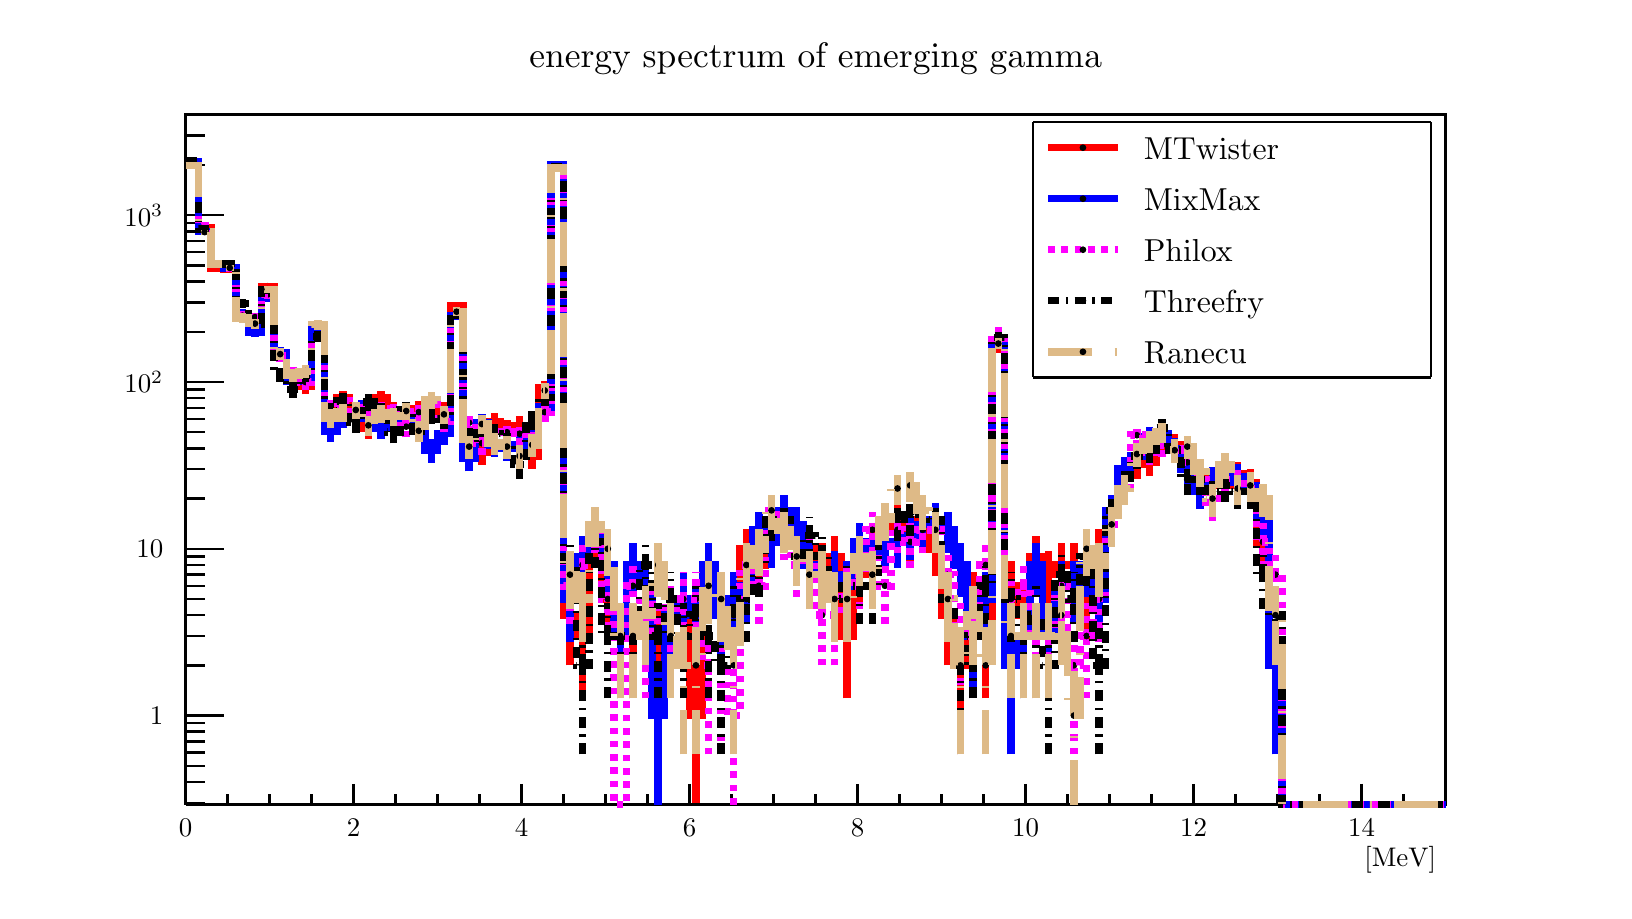
\begin{tikzpicture}
\pgfdeclareplotmark{cross} {
\pgfpathmoveto{\pgfpoint{-0.3\pgfplotmarksize}{\pgfplotmarksize}}
\pgfpathlineto{\pgfpoint{+0.3\pgfplotmarksize}{\pgfplotmarksize}}
\pgfpathlineto{\pgfpoint{+0.3\pgfplotmarksize}{0.3\pgfplotmarksize}}
\pgfpathlineto{\pgfpoint{+1\pgfplotmarksize}{0.3\pgfplotmarksize}}
\pgfpathlineto{\pgfpoint{+1\pgfplotmarksize}{-0.3\pgfplotmarksize}}
\pgfpathlineto{\pgfpoint{+0.3\pgfplotmarksize}{-0.3\pgfplotmarksize}}
\pgfpathlineto{\pgfpoint{+0.3\pgfplotmarksize}{-1.\pgfplotmarksize}}
\pgfpathlineto{\pgfpoint{-0.3\pgfplotmarksize}{-1.\pgfplotmarksize}}
\pgfpathlineto{\pgfpoint{-0.3\pgfplotmarksize}{-0.3\pgfplotmarksize}}
\pgfpathlineto{\pgfpoint{-1.\pgfplotmarksize}{-0.3\pgfplotmarksize}}
\pgfpathlineto{\pgfpoint{-1.\pgfplotmarksize}{0.3\pgfplotmarksize}}
\pgfpathlineto{\pgfpoint{-0.3\pgfplotmarksize}{0.3\pgfplotmarksize}}
\pgfpathclose
\pgfusepathqstroke
}
\pgfdeclareplotmark{cross*} {
\pgfpathmoveto{\pgfpoint{-0.3\pgfplotmarksize}{\pgfplotmarksize}}
\pgfpathlineto{\pgfpoint{+0.3\pgfplotmarksize}{\pgfplotmarksize}}
\pgfpathlineto{\pgfpoint{+0.3\pgfplotmarksize}{0.3\pgfplotmarksize}}
\pgfpathlineto{\pgfpoint{+1\pgfplotmarksize}{0.3\pgfplotmarksize}}
\pgfpathlineto{\pgfpoint{+1\pgfplotmarksize}{-0.3\pgfplotmarksize}}
\pgfpathlineto{\pgfpoint{+0.3\pgfplotmarksize}{-0.3\pgfplotmarksize}}
\pgfpathlineto{\pgfpoint{+0.3\pgfplotmarksize}{-1.\pgfplotmarksize}}
\pgfpathlineto{\pgfpoint{-0.3\pgfplotmarksize}{-1.\pgfplotmarksize}}
\pgfpathlineto{\pgfpoint{-0.3\pgfplotmarksize}{-0.3\pgfplotmarksize}}
\pgfpathlineto{\pgfpoint{-1.\pgfplotmarksize}{-0.3\pgfplotmarksize}}
\pgfpathlineto{\pgfpoint{-1.\pgfplotmarksize}{0.3\pgfplotmarksize}}
\pgfpathlineto{\pgfpoint{-0.3\pgfplotmarksize}{0.3\pgfplotmarksize}}
\pgfpathclose
\pgfusepathqfillstroke
}
\pgfdeclareplotmark{newstar} {
\pgfpathmoveto{\pgfqpoint{0pt}{\pgfplotmarksize}}
\pgfpathlineto{\pgfqpointpolar{44}{0.5\pgfplotmarksize}}
\pgfpathlineto{\pgfqpointpolar{18}{\pgfplotmarksize}}
\pgfpathlineto{\pgfqpointpolar{-20}{0.5\pgfplotmarksize}}
\pgfpathlineto{\pgfqpointpolar{-54}{\pgfplotmarksize}}
\pgfpathlineto{\pgfqpointpolar{-90}{0.5\pgfplotmarksize}}
\pgfpathlineto{\pgfqpointpolar{234}{\pgfplotmarksize}}
\pgfpathlineto{\pgfqpointpolar{198}{0.5\pgfplotmarksize}}
\pgfpathlineto{\pgfqpointpolar{162}{\pgfplotmarksize}}
\pgfpathlineto{\pgfqpointpolar{134}{0.5\pgfplotmarksize}}
\pgfpathclose
\pgfusepathqstroke
}
\pgfdeclareplotmark{newstar*} {
\pgfpathmoveto{\pgfqpoint{0pt}{\pgfplotmarksize}}
\pgfpathlineto{\pgfqpointpolar{44}{0.5\pgfplotmarksize}}
\pgfpathlineto{\pgfqpointpolar{18}{\pgfplotmarksize}}
\pgfpathlineto{\pgfqpointpolar{-20}{0.5\pgfplotmarksize}}
\pgfpathlineto{\pgfqpointpolar{-54}{\pgfplotmarksize}}
\pgfpathlineto{\pgfqpointpolar{-90}{0.5\pgfplotmarksize}}
\pgfpathlineto{\pgfqpointpolar{234}{\pgfplotmarksize}}
\pgfpathlineto{\pgfqpointpolar{198}{0.5\pgfplotmarksize}}
\pgfpathlineto{\pgfqpointpolar{162}{\pgfplotmarksize}}
\pgfpathlineto{\pgfqpointpolar{134}{0.5\pgfplotmarksize}}
\pgfpathclose
\pgfusepathqfillstroke
}
\definecolor{c}{rgb}{1,1,1};
\draw [color=c, fill=c] (0,0) rectangle (20,10.9543);
\draw [color=c, fill=c] (2,1.09543) rectangle (18,9.85885);
\definecolor{c}{rgb}{0,0,0};
\draw [c,line width=0.9] (2,1.09543) -- (2,9.85885) -- (18,9.85885) -- (18,1.09543) -- (2,1.09543);
\definecolor{c}{rgb}{1,1,1};
\draw [color=c, fill=c] (2,1.09543) rectangle (18,9.85885);
\definecolor{c}{rgb}{0,0,0};
\draw [c,line width=0.9] (2,1.09543) -- (2,9.85885) -- (18,9.85885) -- (18,1.09543) -- (2,1.09543);
\definecolor{c}{rgb}{1,0,0};
\draw [c,line width=2.7] (2.08,9.2306) -- (2.08,9.25101);
\draw [c,line width=2.7] (2.08,9.25101) -- (2.08,9.27098);
\definecolor{c}{rgb}{0,0,0};
\foreach \P in {(2.08,9.25101)}{\draw[mark options={color=c,fill=c},mark size=2.402402pt,mark=*,mark size=1pt] plot coordinates {\P};}
\definecolor{c}{rgb}{1,0,0};
\draw [c,line width=2.7] (2.24,8.38866) -- (2.24,8.42092);
\draw [c,line width=2.7] (2.24,8.42092) -- (2.24,8.45208);
\definecolor{c}{rgb}{0,0,0};
\foreach \P in {(2.24,8.42092)}{\draw[mark options={color=c,fill=c},mark size=2.402402pt,mark=*,mark size=1pt] plot coordinates {\P};}
\definecolor{c}{rgb}{1,0,0};
\draw [c,line width=2.7] (2.4,7.86099) -- (2.4,7.90396);
\draw [c,line width=2.7] (2.4,7.90396) -- (2.4,7.94502);
\definecolor{c}{rgb}{0,0,0};
\foreach \P in {(2.4,7.90396)}{\draw[mark options={color=c,fill=c},mark size=2.402402pt,mark=*,mark size=1pt] plot coordinates {\P};}
\definecolor{c}{rgb}{1,0,0};
\draw [c,line width=2.7] (2.56,7.84914) -- (2.56,7.89239);
\draw [c,line width=2.7] (2.56,7.89239) -- (2.56,7.9337);
\definecolor{c}{rgb}{0,0,0};
\foreach \P in {(2.56,7.89239)}{\draw[mark options={color=c,fill=c},mark size=2.402402pt,mark=*,mark size=1pt] plot coordinates {\P};}
\definecolor{c}{rgb}{1,0,0};
\draw [c,line width=2.7] (2.72,7.24762) -- (2.72,7.30759);
\draw [c,line width=2.7] (2.72,7.30759) -- (2.72,7.36389);
\definecolor{c}{rgb}{0,0,0};
\foreach \P in {(2.72,7.30759)}{\draw[mark options={color=c,fill=c},mark size=2.402402pt,mark=*,mark size=1pt] plot coordinates {\P};}
\definecolor{c}{rgb}{1,0,0};
\draw [c,line width=2.7] (2.88,7.22461) -- (2.88,7.28533);
\draw [c,line width=2.7] (2.88,7.28533) -- (2.88,7.3423);
\definecolor{c}{rgb}{0,0,0};
\foreach \P in {(2.88,7.28533)}{\draw[mark options={color=c,fill=c},mark size=2.402402pt,mark=*,mark size=1pt] plot coordinates {\P};}
\definecolor{c}{rgb}{1,0,0};
\draw [c,line width=2.7] (3.04,7.62812) -- (3.04,7.67689);
\draw [c,line width=2.7] (3.04,7.67689) -- (3.04,7.7232);
\definecolor{c}{rgb}{0,0,0};
\foreach \P in {(3.04,7.67689)}{\draw[mark options={color=c,fill=c},mark size=2.402402pt,mark=*,mark size=1pt] plot coordinates {\P};}
\definecolor{c}{rgb}{1,0,0};
\draw [c,line width=2.7] (3.2,6.7231) -- (3.2,6.80285);
\draw [c,line width=2.7] (3.2,6.80285) -- (3.2,6.87623);
\definecolor{c}{rgb}{0,0,0};
\foreach \P in {(3.2,6.80285)}{\draw[mark options={color=c,fill=c},mark size=2.402402pt,mark=*,mark size=1pt] plot coordinates {\P};}
\definecolor{c}{rgb}{1,0,0};
\draw [c,line width=2.7] (3.36,6.44772) -- (3.36,6.54033);
\draw [c,line width=2.7] (3.36,6.54033) -- (3.36,6.62447);
\definecolor{c}{rgb}{0,0,0};
\foreach \P in {(3.36,6.54033)}{\draw[mark options={color=c,fill=c},mark size=2.402402pt,mark=*,mark size=1pt] plot coordinates {\P};}
\definecolor{c}{rgb}{1,0,0};
\draw [c,line width=2.7] (3.52,6.30401) -- (3.52,6.40415);
\draw [c,line width=2.7] (3.52,6.40415) -- (3.52,6.49444);
\definecolor{c}{rgb}{0,0,0};
\foreach \P in {(3.52,6.40415)}{\draw[mark options={color=c,fill=c},mark size=2.402402pt,mark=*,mark size=1pt] plot coordinates {\P};}
\definecolor{c}{rgb}{1,0,0};
\draw [c,line width=2.7] (3.68,6.97208) -- (3.68,7.04174);
\draw [c,line width=2.7] (3.68,7.04174) -- (3.68,7.1065);
\definecolor{c}{rgb}{0,0,0};
\foreach \P in {(3.68,7.04174)}{\draw[mark options={color=c,fill=c},mark size=2.402402pt,mark=*,mark size=1pt] plot coordinates {\P};}
\definecolor{c}{rgb}{1,0,0};
\draw [c,line width=2.7] (3.84,6.00174) -- (3.84,6.11974);
\draw [c,line width=2.7] (3.84,6.11974) -- (3.84,6.2243);
\definecolor{c}{rgb}{0,0,0};
\foreach \P in {(3.84,6.11974)}{\draw[mark options={color=c,fill=c},mark size=2.402402pt,mark=*,mark size=1pt] plot coordinates {\P};}
\definecolor{c}{rgb}{1,0,0};
\draw [c,line width=2.7] (4,6.14674) -- (4,6.2558);
\draw [c,line width=2.7] (4,6.2558) -- (4,6.35329);
\definecolor{c}{rgb}{0,0,0};
\foreach \P in {(4,6.2558)}{\draw[mark options={color=c,fill=c},mark size=2.402402pt,mark=*,mark size=1pt] plot coordinates {\P};}
\definecolor{c}{rgb}{1,0,0};
\draw [c,line width=2.7] (4.16,5.8964) -- (4.16,6.02134);
\draw [c,line width=2.7] (4.16,6.02134) -- (4.16,6.13131);
\definecolor{c}{rgb}{0,0,0};
\foreach \P in {(4.16,6.02134)}{\draw[mark options={color=c,fill=c},mark size=2.402402pt,mark=*,mark size=1pt] plot coordinates {\P};}
\definecolor{c}{rgb}{1,0,0};
\draw [c,line width=2.7] (4.32,5.74115) -- (4.32,5.87706);
\draw [c,line width=2.7] (4.32,5.87706) -- (4.32,5.99546);
\definecolor{c}{rgb}{0,0,0};
\foreach \P in {(4.32,5.87706)}{\draw[mark options={color=c,fill=c},mark size=2.402402pt,mark=*,mark size=1pt] plot coordinates {\P};}
\definecolor{c}{rgb}{1,0,0};
\draw [c,line width=2.7] (4.48,6.14674) -- (4.48,6.2558);
\draw [c,line width=2.7] (4.48,6.2558) -- (4.48,6.35329);
\definecolor{c}{rgb}{0,0,0};
\foreach \P in {(4.48,6.2558)}{\draw[mark options={color=c,fill=c},mark size=2.402402pt,mark=*,mark size=1pt] plot coordinates {\P};}
\definecolor{c}{rgb}{1,0,0};
\draw [c,line width=2.7] (4.64,5.98739) -- (4.64,6.10631);
\draw [c,line width=2.7] (4.64,6.10631) -- (4.64,6.21159);
\definecolor{c}{rgb}{0,0,0};
\foreach \P in {(4.64,6.10631)}{\draw[mark options={color=c,fill=c},mark size=2.402402pt,mark=*,mark size=1pt] plot coordinates {\P};}
\definecolor{c}{rgb}{1,0,0};
\draw [c,line width=2.7] (4.8,5.86403) -- (4.8,5.99118);
\draw [c,line width=2.7] (4.8,5.99118) -- (4.8,6.10286);
\definecolor{c}{rgb}{0,0,0};
\foreach \P in {(4.8,5.99118)}{\draw[mark options={color=c,fill=c},mark size=2.402402pt,mark=*,mark size=1pt] plot coordinates {\P};}
\definecolor{c}{rgb}{1,0,0};
\draw [c,line width=2.7] (4.96,6.00174) -- (4.96,6.11974);
\draw [c,line width=2.7] (4.96,6.11974) -- (4.96,6.2243);
\definecolor{c}{rgb}{0,0,0};
\foreach \P in {(4.96,6.11974)}{\draw[mark options={color=c,fill=c},mark size=2.402402pt,mark=*,mark size=1pt] plot coordinates {\P};}
\definecolor{c}{rgb}{1,0,0};
\draw [c,line width=2.7] (5.12,5.92771) -- (5.12,6.05054);
\draw [c,line width=2.7] (5.12,6.05054) -- (5.12,6.15889);
\definecolor{c}{rgb}{0,0,0};
\foreach \P in {(5.12,6.05054)}{\draw[mark options={color=c,fill=c},mark size=2.402402pt,mark=*,mark size=1pt] plot coordinates {\P};}
\definecolor{c}{rgb}{1,0,0};
\draw [c,line width=2.7] (5.28,5.98739) -- (5.28,6.10631);
\draw [c,line width=2.7] (5.28,6.10631) -- (5.28,6.21159);
\definecolor{c}{rgb}{0,0,0};
\foreach \P in {(5.28,6.10631)}{\draw[mark options={color=c,fill=c},mark size=2.402402pt,mark=*,mark size=1pt] plot coordinates {\P};}
\definecolor{c}{rgb}{1,0,0};
\draw [c,line width=2.7] (5.44,7.36828) -- (5.44,7.42445);
\draw [c,line width=2.7] (5.44,7.42445) -- (5.44,7.47738);
\definecolor{c}{rgb}{0,0,0};
\foreach \P in {(5.44,7.42445)}{\draw[mark options={color=c,fill=c},mark size=2.402402pt,mark=*,mark size=1pt] plot coordinates {\P};}
\definecolor{c}{rgb}{1,0,0};
\draw [c,line width=2.7] (5.6,5.53253) -- (5.6,5.68473);
\draw [c,line width=2.7] (5.6,5.68473) -- (5.6,5.81529);
\definecolor{c}{rgb}{0,0,0};
\foreach \P in {(5.6,5.68473)}{\draw[mark options={color=c,fill=c},mark size=2.402402pt,mark=*,mark size=1pt] plot coordinates {\P};}
\definecolor{c}{rgb}{1,0,0};
\draw [c,line width=2.7] (5.76,5.40821) -- (5.76,5.57102);
\draw [c,line width=2.7] (5.76,5.57102) -- (5.76,5.70931);
\definecolor{c}{rgb}{0,0,0};
\foreach \P in {(5.76,5.57102)}{\draw[mark options={color=c,fill=c},mark size=2.402402pt,mark=*,mark size=1pt] plot coordinates {\P};}
\definecolor{c}{rgb}{1,0,0};
\draw [c,line width=2.7] (5.92,5.83051) -- (5.92,5.95999);
\draw [c,line width=2.7] (5.92,5.95999) -- (5.92,6.07348);
\definecolor{c}{rgb}{0,0,0};
\foreach \P in {(5.92,5.95999)}{\draw[mark options={color=c,fill=c},mark size=2.402402pt,mark=*,mark size=1pt] plot coordinates {\P};}
\definecolor{c}{rgb}{1,0,0};
\draw [c,line width=2.7] (6.08,5.72222) -- (6.08,5.85954);
\draw [c,line width=2.7] (6.08,5.85954) -- (6.08,5.979);
\definecolor{c}{rgb}{0,0,0};
\foreach \P in {(6.08,5.85954)}{\draw[mark options={color=c,fill=c},mark size=2.402402pt,mark=*,mark size=1pt] plot coordinates {\P};}
\definecolor{c}{rgb}{1,0,0};
\draw [c,line width=2.7] (6.24,5.7779) -- (6.24,5.91114);
\draw [c,line width=2.7] (6.24,5.91114) -- (6.24,6.02749);
\definecolor{c}{rgb}{0,0,0};
\foreach \P in {(6.24,5.91114)}{\draw[mark options={color=c,fill=c},mark size=2.402402pt,mark=*,mark size=1pt] plot coordinates {\P};}
\definecolor{c}{rgb}{1,0,0};
\draw [c,line width=2.7] (6.4,5.35358) -- (6.4,5.52129);
\draw [c,line width=2.7] (6.4,5.52129) -- (6.4,5.66309);
\definecolor{c}{rgb}{0,0,0};
\foreach \P in {(6.4,5.52129)}{\draw[mark options={color=c,fill=c},mark size=2.402402pt,mark=*,mark size=1pt] plot coordinates {\P};}
\definecolor{c}{rgb}{1,0,0};
\draw [c,line width=2.7] (6.56,6.28308) -- (6.56,6.38436);
\draw [c,line width=2.7] (6.56,6.38436) -- (6.56,6.47559);
\definecolor{c}{rgb}{0,0,0};
\foreach \P in {(6.56,6.38436)}{\draw[mark options={color=c,fill=c},mark size=2.402402pt,mark=*,mark size=1pt] plot coordinates {\P};}
\definecolor{c}{rgb}{1,0,0};
\draw [c,line width=2.7] (6.72,9.18467) -- (6.72,9.2056);
\draw [c,line width=2.7] (6.72,9.2056) -- (6.72,9.22607);
\definecolor{c}{rgb}{0,0,0};
\foreach \P in {(6.72,9.2056)}{\draw[mark options={color=c,fill=c},mark size=2.402402pt,mark=*,mark size=1pt] plot coordinates {\P};}
\definecolor{c}{rgb}{1,0,0};
\draw [c,line width=2.7] (6.88,2.86256) -- (6.88,3.50016);
\draw [c,line width=2.7] (6.88,3.50016) -- (6.88,3.87313);
\definecolor{c}{rgb}{0,0,0};
\foreach \P in {(6.88,3.50016)}{\draw[mark options={color=c,fill=c},mark size=2.402402pt,mark=*,mark size=1pt] plot coordinates {\P};}
\definecolor{c}{rgb}{1,0,0};
\draw [c,line width=2.7] (7.04,2.44334) -- (7.04,3.23553);
\draw [c,line width=2.7] (7.04,3.23553) -- (7.04,3.65475);
\definecolor{c}{rgb}{0,0,0};
\foreach \P in {(7.04,3.23553)}{\draw[mark options={color=c,fill=c},mark size=2.402402pt,mark=*,mark size=1pt] plot coordinates {\P};}
\definecolor{c}{rgb}{1,0,0};
\draw [c,line width=2.7] (7.2,4.10061) -- (7.2,4.43068);
\draw [c,line width=2.7] (7.2,4.43068) -- (7.2,4.67309);
\definecolor{c}{rgb}{0,0,0};
\foreach \P in {(7.2,4.43068)}{\draw[mark options={color=c,fill=c},mark size=2.402402pt,mark=*,mark size=1pt] plot coordinates {\P};}
\definecolor{c}{rgb}{1,0,0};
\draw [c,line width=2.7] (7.36,3.16014) -- (7.36,3.70542);
\draw [c,line width=2.7] (7.36,3.70542) -- (7.36,4.04543);
\definecolor{c}{rgb}{0,0,0};
\foreach \P in {(7.36,3.70542)}{\draw[mark options={color=c,fill=c},mark size=2.402402pt,mark=*,mark size=1pt] plot coordinates {\P};}
\definecolor{c}{rgb}{1,0,0};
\draw [c,line width=2.7] (7.52,2.44334) -- (7.52,3.23553);
\draw [c,line width=2.7] (7.52,3.23553) -- (7.52,3.65475);
\definecolor{c}{rgb}{0,0,0};
\foreach \P in {(7.52,3.23553)}{\draw[mark options={color=c,fill=c},mark size=2.402402pt,mark=*,mark size=1pt] plot coordinates {\P};}
\definecolor{c}{rgb}{1,0,0};
\draw [c,line width=2.7] (7.68,2.44334) -- (7.68,3.23553);
\draw [c,line width=2.7] (7.68,3.23553) -- (7.68,3.65475);
\definecolor{c}{rgb}{0,0,0};
\foreach \P in {(7.68,3.23553)}{\draw[mark options={color=c,fill=c},mark size=2.402402pt,mark=*,mark size=1pt] plot coordinates {\P};}
\definecolor{c}{rgb}{1,0,0};
\draw [c,line width=2.7] (7.84,2.86256) -- (7.84,3.50016);
\draw [c,line width=2.7] (7.84,3.50016) -- (7.84,3.87313);
\definecolor{c}{rgb}{0,0,0};
\foreach \P in {(7.84,3.50016)}{\draw[mark options={color=c,fill=c},mark size=2.402402pt,mark=*,mark size=1pt] plot coordinates {\P};}
\definecolor{c}{rgb}{1,0,0};
\draw [c,line width=2.7] (8,2.44334) -- (8,3.23553);
\draw [c,line width=2.7] (8,3.23553) -- (8,3.65475);
\definecolor{c}{rgb}{0,0,0};
\foreach \P in {(8,3.23553)}{\draw[mark options={color=c,fill=c},mark size=2.402402pt,mark=*,mark size=1pt] plot coordinates {\P};}
\definecolor{c}{rgb}{1,0,0};
\draw [c,line width=2.7] (8.16,2.86256) -- (8.16,3.50016);
\draw [c,line width=2.7] (8.16,3.50016) -- (8.16,3.87313);
\definecolor{c}{rgb}{0,0,0};
\foreach \P in {(8.16,3.50016)}{\draw[mark options={color=c,fill=c},mark size=2.402402pt,mark=*,mark size=1pt] plot coordinates {\P};}
\definecolor{c}{rgb}{1,0,0};
\draw [c,line width=2.7] (8.32,3.16014) -- (8.32,3.70542);
\draw [c,line width=2.7] (8.32,3.70542) -- (8.32,4.04543);
\definecolor{c}{rgb}{0,0,0};
\foreach \P in {(8.32,3.70542)}{\draw[mark options={color=c,fill=c},mark size=2.402402pt,mark=*,mark size=1pt] plot coordinates {\P};}
\definecolor{c}{rgb}{1,0,0};
\draw [c,line width=2.7] (8.48,1.09543) -- (8.48,2.22496);
\draw [c,line width=2.7] (8.48,2.22496) -- (8.48,2.86256);
\definecolor{c}{rgb}{0,0,0};
\foreach \P in {(8.48,2.22496)}{\draw[mark options={color=c,fill=c},mark size=2.402402pt,mark=*,mark size=1pt] plot coordinates {\P};}
\definecolor{c}{rgb}{1,0,0};
\draw [c,line width=2.7] (8.64,3.39051) -- (8.64,3.87313);
\draw [c,line width=2.7] (8.64,3.87313) -- (8.64,4.18804);
\definecolor{c}{rgb}{0,0,0};
\foreach \P in {(8.64,3.87313)}{\draw[mark options={color=c,fill=c},mark size=2.402402pt,mark=*,mark size=1pt] plot coordinates {\P};}
\definecolor{c}{rgb}{1,0,0};
\draw [c,line width=2.7] (8.8,3.16014) -- (8.8,3.70542);
\draw [c,line width=2.7] (8.8,3.70542) -- (8.8,4.04543);
\definecolor{c}{rgb}{0,0,0};
\foreach \P in {(8.8,3.70542)}{\draw[mark options={color=c,fill=c},mark size=2.402402pt,mark=*,mark size=1pt] plot coordinates {\P};}
\definecolor{c}{rgb}{1,0,0};
\draw [c,line width=2.7] (8.96,2.86256) -- (8.96,3.50016);
\draw [c,line width=2.7] (8.96,3.50016) -- (8.96,3.87313);
\definecolor{c}{rgb}{0,0,0};
\foreach \P in {(8.96,3.50016)}{\draw[mark options={color=c,fill=c},mark size=2.402402pt,mark=*,mark size=1pt] plot coordinates {\P};}
\definecolor{c}{rgb}{1,0,0};
\draw [c,line width=2.7] (9.12,3.99335) -- (9.12,4.34301);
\draw [c,line width=2.7] (9.12,4.34301) -- (9.12,4.59576);
\definecolor{c}{rgb}{0,0,0};
\foreach \P in {(9.12,4.34301)}{\draw[mark options={color=c,fill=c},mark size=2.402402pt,mark=*,mark size=1pt] plot coordinates {\P};}
\definecolor{c}{rgb}{1,0,0};
\draw [c,line width=2.7] (9.28,3.73645) -- (9.28,4.13775);
\draw [c,line width=2.7] (9.28,4.13775) -- (9.28,4.41622);
\definecolor{c}{rgb}{0,0,0};
\foreach \P in {(9.28,4.13775)}{\draw[mark options={color=c,fill=c},mark size=2.402402pt,mark=*,mark size=1pt] plot coordinates {\P};}
\definecolor{c}{rgb}{1,0,0};
\draw [c,line width=2.7] (9.44,4.28555) -- (9.44,4.58435);
\draw [c,line width=2.7] (9.44,4.58435) -- (9.44,4.80952);
\definecolor{c}{rgb}{0,0,0};
\foreach \P in {(9.44,4.58435)}{\draw[mark options={color=c,fill=c},mark size=2.402402pt,mark=*,mark size=1pt] plot coordinates {\P};}
\definecolor{c}{rgb}{1,0,0};
\draw [c,line width=2.7] (9.6,4.28555) -- (9.6,4.58435);
\draw [c,line width=2.7] (9.6,4.58435) -- (9.6,4.80952);
\definecolor{c}{rgb}{0,0,0};
\foreach \P in {(9.6,4.58435)}{\draw[mark options={color=c,fill=c},mark size=2.402402pt,mark=*,mark size=1pt] plot coordinates {\P};}
\definecolor{c}{rgb}{1,0,0};
\draw [c,line width=2.7] (9.76,4.1974) -- (9.76,4.51072);
\draw [c,line width=2.7] (9.76,4.51072) -- (9.76,4.74401);
\definecolor{c}{rgb}{0,0,0};
\foreach \P in {(9.76,4.51072)}{\draw[mark options={color=c,fill=c},mark size=2.402402pt,mark=*,mark size=1pt] plot coordinates {\P};}
\definecolor{c}{rgb}{1,0,0};
\draw [c,line width=2.7] (9.92,3.99335) -- (9.92,4.34301);
\draw [c,line width=2.7] (9.92,4.34301) -- (9.92,4.59576);
\definecolor{c}{rgb}{0,0,0};
\foreach \P in {(9.92,4.34301)}{\draw[mark options={color=c,fill=c},mark size=2.402402pt,mark=*,mark size=1pt] plot coordinates {\P};}
\definecolor{c}{rgb}{1,0,0};
\draw [c,line width=2.7] (10.08,3.73645) -- (10.08,4.13775);
\draw [c,line width=2.7] (10.08,4.13775) -- (10.08,4.41622);
\definecolor{c}{rgb}{0,0,0};
\foreach \P in {(10.08,4.13775)}{\draw[mark options={color=c,fill=c},mark size=2.402402pt,mark=*,mark size=1pt] plot coordinates {\P};}
\definecolor{c}{rgb}{1,0,0};
\draw [c,line width=2.7] (10.24,3.87313) -- (10.24,4.2461);
\draw [c,line width=2.7] (10.24,4.2461) -- (10.24,4.51072);
\definecolor{c}{rgb}{0,0,0};
\foreach \P in {(10.24,4.2461)}{\draw[mark options={color=c,fill=c},mark size=2.402402pt,mark=*,mark size=1pt] plot coordinates {\P};}
\definecolor{c}{rgb}{1,0,0};
\draw [c,line width=2.7] (10.4,2.44334) -- (10.4,3.23553);
\draw [c,line width=2.7] (10.4,3.23553) -- (10.4,3.65475);
\definecolor{c}{rgb}{0,0,0};
\foreach \P in {(10.4,3.23553)}{\draw[mark options={color=c,fill=c},mark size=2.402402pt,mark=*,mark size=1pt] plot coordinates {\P};}
\definecolor{c}{rgb}{1,0,0};
\draw [c,line width=2.7] (10.56,3.57821) -- (10.56,4.01492);
\draw [c,line width=2.7] (10.56,4.01492) -- (10.56,4.30984);
\definecolor{c}{rgb}{0,0,0};
\foreach \P in {(10.56,4.01492)}{\draw[mark options={color=c,fill=c},mark size=2.402402pt,mark=*,mark size=1pt] plot coordinates {\P};}
\definecolor{c}{rgb}{1,0,0};
\draw [c,line width=2.7] (10.72,3.99335) -- (10.72,4.34301);
\draw [c,line width=2.7] (10.72,4.34301) -- (10.72,4.59576);
\definecolor{c}{rgb}{0,0,0};
\foreach \P in {(10.72,4.34301)}{\draw[mark options={color=c,fill=c},mark size=2.402402pt,mark=*,mark size=1pt] plot coordinates {\P};}
\definecolor{c}{rgb}{1,0,0};
\draw [c,line width=2.7] (10.88,4.28555) -- (10.88,4.58435);
\draw [c,line width=2.7] (10.88,4.58435) -- (10.88,4.80952);
\definecolor{c}{rgb}{0,0,0};
\foreach \P in {(10.88,4.58435)}{\draw[mark options={color=c,fill=c},mark size=2.402402pt,mark=*,mark size=1pt] plot coordinates {\P};}
\definecolor{c}{rgb}{1,0,0};
\draw [c,line width=2.7] (11.04,4.44125) -- (11.04,4.71598);
\draw [c,line width=2.7] (11.04,4.71598) -- (11.04,4.92726);
\definecolor{c}{rgb}{0,0,0};
\foreach \P in {(11.04,4.71598)}{\draw[mark options={color=c,fill=c},mark size=2.402402pt,mark=*,mark size=1pt] plot coordinates {\P};}
\definecolor{c}{rgb}{1,0,0};
\draw [c,line width=2.7] (11.2,4.10061) -- (11.2,4.43068);
\draw [c,line width=2.7] (11.2,4.43068) -- (11.2,4.67309);
\definecolor{c}{rgb}{0,0,0};
\foreach \P in {(11.2,4.43068)}{\draw[mark options={color=c,fill=c},mark size=2.402402pt,mark=*,mark size=1pt] plot coordinates {\P};}
\definecolor{c}{rgb}{1,0,0};
\draw [c,line width=2.7] (11.36,4.44125) -- (11.36,4.71598);
\draw [c,line width=2.7] (11.36,4.71598) -- (11.36,4.92726);
\definecolor{c}{rgb}{0,0,0};
\foreach \P in {(11.36,4.71598)}{\draw[mark options={color=c,fill=c},mark size=2.402402pt,mark=*,mark size=1pt] plot coordinates {\P};}
\definecolor{c}{rgb}{1,0,0};
\draw [c,line width=2.7] (11.52,3.99335) -- (11.52,4.34301);
\draw [c,line width=2.7] (11.52,4.34301) -- (11.52,4.59576);
\definecolor{c}{rgb}{0,0,0};
\foreach \P in {(11.52,4.34301)}{\draw[mark options={color=c,fill=c},mark size=2.402402pt,mark=*,mark size=1pt] plot coordinates {\P};}
\definecolor{c}{rgb}{1,0,0};
\draw [c,line width=2.7] (11.68,2.86256) -- (11.68,3.50016);
\draw [c,line width=2.7] (11.68,3.50016) -- (11.68,3.87313);
\definecolor{c}{rgb}{0,0,0};
\foreach \P in {(11.68,3.50016)}{\draw[mark options={color=c,fill=c},mark size=2.402402pt,mark=*,mark size=1pt] plot coordinates {\P};}
\definecolor{c}{rgb}{1,0,0};
\draw [c,line width=2.7] (11.84,1.73302) -- (11.84,2.86256);
\draw [c,line width=2.7] (11.84,2.86256) -- (11.84,3.3545);
\definecolor{c}{rgb}{0,0,0};
\foreach \P in {(11.84,2.86256)}{\draw[mark options={color=c,fill=c},mark size=2.402402pt,mark=*,mark size=1pt] plot coordinates {\P};}
\definecolor{c}{rgb}{1,0,0};
\draw [c,line width=2.7] (12,3.16014) -- (12,3.70542);
\draw [c,line width=2.7] (12,3.70542) -- (12,4.04543);
\definecolor{c}{rgb}{0,0,0};
\foreach \P in {(12,3.70542)}{\draw[mark options={color=c,fill=c},mark size=2.402402pt,mark=*,mark size=1pt] plot coordinates {\P};}
\definecolor{c}{rgb}{1,0,0};
\draw [c,line width=2.7] (12.16,2.44334) -- (12.16,3.23553);
\draw [c,line width=2.7] (12.16,3.23553) -- (12.16,3.65475);
\definecolor{c}{rgb}{0,0,0};
\foreach \P in {(12.16,3.23553)}{\draw[mark options={color=c,fill=c},mark size=2.402402pt,mark=*,mark size=1pt] plot coordinates {\P};}
\definecolor{c}{rgb}{1,0,0};
\draw [c,line width=2.7] (12.32,6.82362) -- (12.32,6.89913);
\draw [c,line width=2.7] (12.32,6.89913) -- (12.32,6.96891);
\definecolor{c}{rgb}{0,0,0};
\foreach \P in {(12.32,6.89913)}{\draw[mark options={color=c,fill=c},mark size=2.402402pt,mark=*,mark size=1pt] plot coordinates {\P};}
\definecolor{c}{rgb}{1,0,0};
\draw [c,line width=2.7] (12.48,3.39051) -- (12.48,3.87313);
\draw [c,line width=2.7] (12.48,3.87313) -- (12.48,4.18804);
\definecolor{c}{rgb}{0,0,0};
\foreach \P in {(12.48,3.87313)}{\draw[mark options={color=c,fill=c},mark size=2.402402pt,mark=*,mark size=1pt] plot coordinates {\P};}
\definecolor{c}{rgb}{1,0,0};
\draw [c,line width=2.7] (12.64,2.86256) -- (12.64,3.50016);
\draw [c,line width=2.7] (12.64,3.50016) -- (12.64,3.87313);
\definecolor{c}{rgb}{0,0,0};
\foreach \P in {(12.64,3.50016)}{\draw[mark options={color=c,fill=c},mark size=2.402402pt,mark=*,mark size=1pt] plot coordinates {\P};}
\definecolor{c}{rgb}{1,0,0};
\draw [c,line width=2.7] (12.8,3.87313) -- (12.8,4.2461);
\draw [c,line width=2.7] (12.8,4.2461) -- (12.8,4.51072);
\definecolor{c}{rgb}{0,0,0};
\foreach \P in {(12.8,4.2461)}{\draw[mark options={color=c,fill=c},mark size=2.402402pt,mark=*,mark size=1pt] plot coordinates {\P};}
\definecolor{c}{rgb}{1,0,0};
\draw [c,line width=2.7] (12.96,3.57821) -- (12.96,4.01492);
\draw [c,line width=2.7] (12.96,4.01492) -- (12.96,4.30984);
\definecolor{c}{rgb}{0,0,0};
\foreach \P in {(12.96,4.01492)}{\draw[mark options={color=c,fill=c},mark size=2.402402pt,mark=*,mark size=1pt] plot coordinates {\P};}
\definecolor{c}{rgb}{1,0,0};
\draw [c,line width=2.7] (13.12,3.73645) -- (13.12,4.13775);
\draw [c,line width=2.7] (13.12,4.13775) -- (13.12,4.41622);
\definecolor{c}{rgb}{0,0,0};
\foreach \P in {(13.12,4.13775)}{\draw[mark options={color=c,fill=c},mark size=2.402402pt,mark=*,mark size=1pt] plot coordinates {\P};}
\definecolor{c}{rgb}{1,0,0};
\draw [c,line width=2.7] (13.28,3.73645) -- (13.28,4.13775);
\draw [c,line width=2.7] (13.28,4.13775) -- (13.28,4.41622);
\definecolor{c}{rgb}{0,0,0};
\foreach \P in {(13.28,4.13775)}{\draw[mark options={color=c,fill=c},mark size=2.402402pt,mark=*,mark size=1pt] plot coordinates {\P};}
\definecolor{c}{rgb}{1,0,0};
\draw [c,line width=2.7] (13.44,3.16014) -- (13.44,3.70542);
\draw [c,line width=2.7] (13.44,3.70542) -- (13.44,4.04543);
\definecolor{c}{rgb}{0,0,0};
\foreach \P in {(13.44,3.70542)}{\draw[mark options={color=c,fill=c},mark size=2.402402pt,mark=*,mark size=1pt] plot coordinates {\P};}
\definecolor{c}{rgb}{1,0,0};
\draw [c,line width=2.7] (13.6,3.99335) -- (13.6,4.34301);
\draw [c,line width=2.7] (13.6,4.34301) -- (13.6,4.59576);
\definecolor{c}{rgb}{0,0,0};
\foreach \P in {(13.6,4.34301)}{\draw[mark options={color=c,fill=c},mark size=2.402402pt,mark=*,mark size=1pt] plot coordinates {\P};}
\definecolor{c}{rgb}{1,0,0};
\draw [c,line width=2.7] (13.76,4.5756) -- (13.76,4.83111);
\draw [c,line width=2.7] (13.76,4.83111) -- (13.76,5.03087);
\definecolor{c}{rgb}{0,0,0};
\foreach \P in {(13.76,4.83111)}{\draw[mark options={color=c,fill=c},mark size=2.402402pt,mark=*,mark size=1pt] plot coordinates {\P};}
\definecolor{c}{rgb}{1,0,0};
\draw [c,line width=2.7] (13.92,5.16814) -- (13.92,5.35358);
\draw [c,line width=2.7] (13.92,5.35358) -- (13.92,5.50783);
\definecolor{c}{rgb}{0,0,0};
\foreach \P in {(13.92,5.35358)}{\draw[mark options={color=c,fill=c},mark size=2.402402pt,mark=*,mark size=1pt] plot coordinates {\P};}
\definecolor{c}{rgb}{1,0,0};
\draw [c,line width=2.7] (14.08,5.23401) -- (14.08,5.41295);
\draw [c,line width=2.7] (14.08,5.41295) -- (14.08,5.56268);
\definecolor{c}{rgb}{0,0,0};
\foreach \P in {(14.08,5.41295)}{\draw[mark options={color=c,fill=c},mark size=2.402402pt,mark=*,mark size=1pt] plot coordinates {\P};}
\definecolor{c}{rgb}{1,0,0};
\draw [c,line width=2.7] (14.24,5.26532) -- (14.24,5.44125);
\draw [c,line width=2.7] (14.24,5.44125) -- (14.24,5.58887);
\definecolor{c}{rgb}{0,0,0};
\foreach \P in {(14.24,5.44125)}{\draw[mark options={color=c,fill=c},mark size=2.402402pt,mark=*,mark size=1pt] plot coordinates {\P};}
\definecolor{c}{rgb}{1,0,0};
\draw [c,line width=2.7] (14.4,5.60004) -- (14.4,5.74677);
\draw [c,line width=2.7] (14.4,5.74677) -- (14.4,5.87328);
\definecolor{c}{rgb}{0,0,0};
\foreach \P in {(14.4,5.74677)}{\draw[mark options={color=c,fill=c},mark size=2.402402pt,mark=*,mark size=1pt] plot coordinates {\P};}
\definecolor{c}{rgb}{1,0,0};
\draw [c,line width=2.7] (14.56,5.50892) -- (14.56,5.66309);
\draw [c,line width=2.7] (14.56,5.66309) -- (14.56,5.79508);
\definecolor{c}{rgb}{0,0,0};
\foreach \P in {(14.56,5.66309)}{\draw[mark options={color=c,fill=c},mark size=2.402402pt,mark=*,mark size=1pt] plot coordinates {\P};}
\definecolor{c}{rgb}{1,0,0};
\draw [c,line width=2.7] (14.72,5.26532) -- (14.72,5.44125);
\draw [c,line width=2.7] (14.72,5.44125) -- (14.72,5.58887);
\definecolor{c}{rgb}{0,0,0};
\foreach \P in {(14.72,5.44125)}{\draw[mark options={color=c,fill=c},mark size=2.402402pt,mark=*,mark size=1pt] plot coordinates {\P};}
\definecolor{c}{rgb}{1,0,0};
\draw [c,line width=2.7] (14.88,5.13344) -- (14.88,5.32239);
\draw [c,line width=2.7] (14.88,5.32239) -- (14.88,5.47907);
\definecolor{c}{rgb}{0,0,0};
\foreach \P in {(14.88,5.32239)}{\draw[mark options={color=c,fill=c},mark size=2.402402pt,mark=*,mark size=1pt] plot coordinates {\P};}
\definecolor{c}{rgb}{1,0,0};
\draw [c,line width=2.7] (15.04,4.98061) -- (15.04,5.18587);
\draw [c,line width=2.7] (15.04,5.18587) -- (15.04,5.35358);
\definecolor{c}{rgb}{0,0,0};
\foreach \P in {(15.04,5.18587)}{\draw[mark options={color=c,fill=c},mark size=2.402402pt,mark=*,mark size=1pt] plot coordinates {\P};}
\definecolor{c}{rgb}{1,0,0};
\draw [c,line width=2.7] (15.2,4.9383) -- (15.2,5.14832);
\draw [c,line width=2.7] (15.2,5.14832) -- (15.2,5.31918);
\definecolor{c}{rgb}{0,0,0};
\foreach \P in {(15.2,5.14832)}{\draw[mark options={color=c,fill=c},mark size=2.402402pt,mark=*,mark size=1pt] plot coordinates {\P};}
\definecolor{c}{rgb}{1,0,0};
\draw [c,line width=2.7] (15.36,5.09744) -- (15.36,5.29012);
\draw [c,line width=2.7] (15.36,5.29012) -- (15.36,5.44934);
\definecolor{c}{rgb}{0,0,0};
\foreach \P in {(15.36,5.29012)}{\draw[mark options={color=c,fill=c},mark size=2.402402pt,mark=*,mark size=1pt] plot coordinates {\P};}
\definecolor{c}{rgb}{1,0,0};
\draw [c,line width=2.7] (15.52,4.98061) -- (15.52,5.18587);
\draw [c,line width=2.7] (15.52,5.18587) -- (15.52,5.35358);
\definecolor{c}{rgb}{0,0,0};
\foreach \P in {(15.52,5.18587)}{\draw[mark options={color=c,fill=c},mark size=2.402402pt,mark=*,mark size=1pt] plot coordinates {\P};}
\definecolor{c}{rgb}{1,0,0};
\draw [c,line width=2.7] (15.68,4.10061) -- (15.68,4.43068);
\draw [c,line width=2.7] (15.68,4.43068) -- (15.68,4.67309);
\definecolor{c}{rgb}{0,0,0};
\foreach \P in {(15.68,4.43068)}{\draw[mark options={color=c,fill=c},mark size=2.402402pt,mark=*,mark size=1pt] plot coordinates {\P};}
\definecolor{c}{rgb}{1,0,0};
\draw [c,line width=2.7] (15.84,1.73302) -- (15.84,2.86256);
\draw [c,line width=2.7] (15.84,2.86256) -- (15.84,3.3545);
\definecolor{c}{rgb}{0,0,0};
\foreach \P in {(15.84,2.86256)}{\draw[mark options={color=c,fill=c},mark size=2.402402pt,mark=*,mark size=1pt] plot coordinates {\P};}
\definecolor{c}{rgb}{1,0,0};
\draw [c,line width=2.7] (2,9.25101) -- (2.16,9.25101) -- (2.16,8.42092) -- (2.32,8.42092) -- (2.32,7.90396) -- (2.48,7.90396) -- (2.48,7.89239) -- (2.64,7.89239) -- (2.64,7.30759) -- (2.8,7.30759) -- (2.8,7.28533) -- (2.96,7.28533) -- (2.96,7.67689)
 -- (3.12,7.67689) -- (3.12,6.80285) -- (3.28,6.80285) -- (3.28,6.54033) -- (3.44,6.54033) -- (3.44,6.40415) -- (3.6,6.40415) -- (3.6,7.04174) -- (3.76,7.04174) -- (3.76,6.11974) -- (3.92,6.11974) -- (3.92,6.2558) -- (4.08,6.2558) -- (4.08,6.02134)
 -- (4.24,6.02134) -- (4.24,5.87706) -- (4.4,5.87706) -- (4.4,6.2558) -- (4.56,6.2558) -- (4.56,6.10631) -- (4.72,6.10631) -- (4.72,5.99118) -- (4.88,5.99118) -- (4.88,6.11974) -- (5.04,6.11974) -- (5.04,6.05054) -- (5.2,6.05054) -- (5.2,6.10631) --
 (5.36,6.10631) -- (5.36,7.42445) -- (5.52,7.42445) -- (5.52,5.68473) -- (5.68,5.68473) -- (5.68,5.57102) -- (5.84,5.57102) -- (5.84,5.95999) -- (6,5.95999) -- (6,5.85954) -- (6.16,5.85954) -- (6.16,5.91114) -- (6.32,5.91114) -- (6.32,5.52129) --
 (6.48,5.52129) -- (6.48,6.38436) -- (6.64,6.38436) -- (6.64,9.2056) -- (6.8,9.2056) -- (6.8,3.50016) -- (6.96,3.50016) -- (6.96,3.23553) -- (7.12,3.23553) -- (7.12,4.43068) -- (7.28,4.43068) -- (7.28,3.70542) -- (7.44,3.70542) -- (7.44,3.23553) --
 (7.6,3.23553) -- (7.6,3.23553) -- (7.76,3.23553) -- (7.76,3.50016) -- (7.92,3.50016) -- (7.92,3.23553) -- (8.08,3.23553) -- (8.08,3.50016) -- (8.24,3.50016) -- (8.24,3.70542) -- (8.4,3.70542) -- (8.4,2.22496) -- (8.56,2.22496) -- (8.56,3.87313) --
 (8.72,3.87313) -- (8.72,3.70542) -- (8.88,3.70542) -- (8.88,3.50016) -- (9.04,3.50016) -- (9.04,4.34301) -- (9.2,4.34301) -- (9.2,4.13775) -- (9.36,4.13775) -- (9.36,4.58435) -- (9.52,4.58435) -- (9.52,4.58435) -- (9.68,4.58435) -- (9.68,4.51072) --
 (9.84,4.51072) -- (9.84,4.34301) -- (10,4.34301) -- (10,4.13775) -- (10.16,4.13775) -- (10.16,4.2461) -- (10.32,4.2461) -- (10.32,3.23553) -- (10.48,3.23553) -- (10.48,4.01492) -- (10.64,4.01492) -- (10.64,4.34301) -- (10.8,4.34301) --
 (10.8,4.58435) -- (10.96,4.58435) -- (10.96,4.71598) -- (11.12,4.71598) -- (11.12,4.43068) -- (11.28,4.43068) -- (11.28,4.71598) -- (11.44,4.71598) -- (11.44,4.34301) -- (11.6,4.34301) -- (11.6,3.50016) -- (11.76,3.50016) -- (11.76,2.86256) --
 (11.92,2.86256) -- (11.92,3.70542) -- (12.08,3.70542) -- (12.08,3.23553) -- (12.24,3.23553) -- (12.24,6.89913) -- (12.4,6.89913) -- (12.4,3.87313) -- (12.56,3.87313) -- (12.56,3.50016) -- (12.72,3.50016) -- (12.72,4.2461) -- (12.88,4.2461) --
 (12.88,4.01492) -- (13.04,4.01492) -- (13.04,4.13775) -- (13.2,4.13775) -- (13.2,4.13775) -- (13.36,4.13775) -- (13.36,3.70542) -- (13.52,3.70542) -- (13.52,4.34301) -- (13.68,4.34301) -- (13.68,4.83111) -- (13.84,4.83111) -- (13.84,5.35358) --
 (14,5.35358) -- (14,5.41295) -- (14.16,5.41295) -- (14.16,5.44125) -- (14.32,5.44125) -- (14.32,5.74677) -- (14.48,5.74677) -- (14.48,5.66309) -- (14.64,5.66309) -- (14.64,5.44125) -- (14.8,5.44125) -- (14.8,5.32239) -- (14.96,5.32239) --
 (14.96,5.18587) -- (15.12,5.18587) -- (15.12,5.14832) -- (15.28,5.14832) -- (15.28,5.29012) -- (15.44,5.29012) -- (15.44,5.18587) -- (15.6,5.18587) -- (15.6,4.43068) -- (15.76,4.43068) -- (15.76,2.86256) -- (15.92,2.86256) -- (15.92,1.09543) --
 (16.08,1.09543) -- (16.08,1.09543) -- (16.24,1.09543) -- (16.24,1.09543) -- (16.4,1.09543) -- (16.4,1.09543) -- (16.56,1.09543) -- (16.56,1.09543) -- (16.72,1.09543) -- (16.72,1.09543) -- (16.88,1.09543) -- (16.88,1.09543) -- (17.04,1.09543) --
 (17.04,1.09543) -- (17.2,1.09543) -- (17.2,1.09543) -- (17.36,1.09543) -- (17.36,1.09543) -- (17.52,1.09543) -- (17.52,1.09543) -- (17.68,1.09543) -- (17.68,1.09543) -- (17.84,1.09543) -- (17.84,1.09543) -- (18,1.09543);
\definecolor{c}{rgb}{0,0,0};
\draw [c,line width=0.9] (2,1.09543) -- (18,1.09543);
\draw [c,line width=0.9] (2,1.35833) -- (2,1.09543);
\draw [c,line width=0.9] (2.53333,1.22688) -- (2.53333,1.09543);
\draw [c,line width=0.9] (3.06667,1.22688) -- (3.06667,1.09543);
\draw [c,line width=0.9] (3.6,1.22688) -- (3.6,1.09543);
\draw [c,line width=0.9] (4.13333,1.35833) -- (4.13333,1.09543);
\draw [c,line width=0.9] (4.66667,1.22688) -- (4.66667,1.09543);
\draw [c,line width=0.9] (5.2,1.22688) -- (5.2,1.09543);
\draw [c,line width=0.9] (5.73333,1.22688) -- (5.73333,1.09543);
\draw [c,line width=0.9] (6.26667,1.35833) -- (6.26667,1.09543);
\draw [c,line width=0.9] (6.8,1.22688) -- (6.8,1.09543);
\draw [c,line width=0.9] (7.33333,1.22688) -- (7.33333,1.09543);
\draw [c,line width=0.9] (7.86667,1.22688) -- (7.86667,1.09543);
\draw [c,line width=0.9] (8.4,1.35833) -- (8.4,1.09543);
\draw [c,line width=0.9] (8.93333,1.22688) -- (8.93333,1.09543);
\draw [c,line width=0.9] (9.46667,1.22688) -- (9.46667,1.09543);
\draw [c,line width=0.9] (10,1.22688) -- (10,1.09543);
\draw [c,line width=0.9] (10.5333,1.35833) -- (10.5333,1.09543);
\draw [c,line width=0.9] (11.0667,1.22688) -- (11.0667,1.09543);
\draw [c,line width=0.9] (11.6,1.22688) -- (11.6,1.09543);
\draw [c,line width=0.9] (12.1333,1.22688) -- (12.1333,1.09543);
\draw [c,line width=0.9] (12.6667,1.35833) -- (12.6667,1.09543);
\draw [c,line width=0.9] (13.2,1.22688) -- (13.2,1.09543);
\draw [c,line width=0.9] (13.7333,1.22688) -- (13.7333,1.09543);
\draw [c,line width=0.9] (14.2667,1.22688) -- (14.2667,1.09543);
\draw [c,line width=0.9] (14.8,1.35833) -- (14.8,1.09543);
\draw [c,line width=0.9] (15.3333,1.22688) -- (15.3333,1.09543);
\draw [c,line width=0.9] (15.8667,1.22688) -- (15.8667,1.09543);
\draw [c,line width=0.9] (16.4,1.22688) -- (16.4,1.09543);
\draw [c,line width=0.9] (16.9333,1.35833) -- (16.9333,1.09543);
\draw [c,line width=0.9] (16.9333,1.35833) -- (16.9333,1.09543);
\draw [c,line width=0.9] (17.4667,1.22688) -- (17.4667,1.09543);
\draw [anchor=base] (2,0.690119) node[scale=0.971398, color=c, rotate=0]{0};
\draw [anchor=base] (4.13333,0.690119) node[scale=0.971398, color=c, rotate=0]{2};
\draw [anchor=base] (6.26667,0.690119) node[scale=0.971398, color=c, rotate=0]{4};
\draw [anchor=base] (8.4,0.690119) node[scale=0.971398, color=c, rotate=0]{6};
\draw [anchor=base] (10.5333,0.690119) node[scale=0.971398, color=c, rotate=0]{8};
\draw [anchor=base] (12.6667,0.690119) node[scale=0.971398, color=c, rotate=0]{10};
\draw [anchor=base] (14.8,0.690119) node[scale=0.971398, color=c, rotate=0]{12};
\draw [anchor=base] (16.9333,0.690119) node[scale=0.971398, color=c, rotate=0]{14};
\draw [anchor= east] (18,0.394354) node[scale=0.971398, color=c, rotate=0]{ [MeV]};
\draw [c,line width=0.9] (2,1.09543) -- (2,9.85885);
\draw [c,line width=0.9] (2.24,1.11748) -- (2,1.11748);
\draw [c,line width=0.9] (2.24,1.38211) -- (2,1.38211);
\draw [c,line width=0.9] (2.24,1.58737) -- (2,1.58737);
\draw [c,line width=0.9] (2.24,1.75508) -- (2,1.75508);
\draw [c,line width=0.9] (2.24,1.89688) -- (2,1.89688);
\draw [c,line width=0.9] (2.24,2.01971) -- (2,2.01971);
\draw [c,line width=0.9] (2.24,2.12805) -- (2,2.12805);
\draw [c,line width=0.9] (2.48,2.22497) -- (2,2.22497);
\draw [anchor= east] (1.836,2.22497) node[scale=0.971398, color=c, rotate=0]{1};
\draw [c,line width=0.9] (2.24,2.86256) -- (2,2.86256);
\draw [c,line width=0.9] (2.24,3.23553) -- (2,3.23553);
\draw [c,line width=0.9] (2.24,3.50016) -- (2,3.50016);
\draw [c,line width=0.9] (2.24,3.70542) -- (2,3.70542);
\draw [c,line width=0.9] (2.24,3.87313) -- (2,3.87313);
\draw [c,line width=0.9] (2.24,4.01492) -- (2,4.01492);
\draw [c,line width=0.9] (2.24,4.13775) -- (2,4.13775);
\draw [c,line width=0.9] (2.24,4.2461) -- (2,4.2461);
\draw [c,line width=0.9] (2.48,4.34301) -- (2,4.34301);
\draw [anchor= east] (1.836,4.34301) node[scale=0.971398, color=c, rotate=0]{10};
\draw [c,line width=0.9] (2.24,4.98061) -- (2,4.98061);
\draw [c,line width=0.9] (2.24,5.35358) -- (2,5.35358);
\draw [c,line width=0.9] (2.24,5.61821) -- (2,5.61821);
\draw [c,line width=0.9] (2.24,5.82347) -- (2,5.82347);
\draw [c,line width=0.9] (2.24,5.99118) -- (2,5.99118);
\draw [c,line width=0.9] (2.24,6.13297) -- (2,6.13297);
\draw [c,line width=0.9] (2.24,6.2558) -- (2,6.2558);
\draw [c,line width=0.9] (2.24,6.36415) -- (2,6.36415);
\draw [c,line width=0.9] (2.48,6.46106) -- (2,6.46106);
\draw [anchor= east] (1.836,6.46106) node[scale=0.971398, color=c, rotate=0]{$10^{2}$};
\draw [c,line width=0.9] (2.24,7.09866) -- (2,7.09866);
\draw [c,line width=0.9] (2.24,7.47163) -- (2,7.47163);
\draw [c,line width=0.9] (2.24,7.73626) -- (2,7.73626);
\draw [c,line width=0.9] (2.24,7.94151) -- (2,7.94151);
\draw [c,line width=0.9] (2.24,8.10923) -- (2,8.10923);
\draw [c,line width=0.9] (2.24,8.25102) -- (2,8.25102);
\draw [c,line width=0.9] (2.24,8.37385) -- (2,8.37385);
\draw [c,line width=0.9] (2.24,8.48219) -- (2,8.48219);
\draw [c,line width=0.9] (2.48,8.57911) -- (2,8.57911);
\draw [anchor= east] (1.836,8.57911) node[scale=0.971398, color=c, rotate=0]{$10^{3}$};
\draw [c,line width=0.9] (2.24,9.21671) -- (2,9.21671);
\draw [c,line width=0.9] (2.24,9.58968) -- (2,9.58968);
\draw [c,line width=0.9] (2.24,9.8543) -- (2,9.8543);
\draw (10,10.5655) node[scale=1.28048, color=c, rotate=0]{energy spectrum of emerging gamma};
\definecolor{c}{rgb}{0,0,1};
\draw [c,line width=2.7] (2.08,9.23552) -- (2.08,9.25588);
\draw [c,line width=2.7] (2.08,9.25588) -- (2.08,9.27579);
\definecolor{c}{rgb}{0,0,0};
\foreach \P in {(2.08,9.25588)}{\draw[mark options={color=c,fill=c},mark size=2.402402pt,mark=*,mark size=1pt] plot coordinates {\P};}
\definecolor{c}{rgb}{0,0,1};
\draw [c,line width=2.7] (2.24,8.34074) -- (2.24,8.37385);
\draw [c,line width=2.7] (2.24,8.37385) -- (2.24,8.40581);
\definecolor{c}{rgb}{0,0,0};
\foreach \P in {(2.24,8.37385)}{\draw[mark options={color=c,fill=c},mark size=2.402402pt,mark=*,mark size=1pt] plot coordinates {\P};}
\definecolor{c}{rgb}{0,0,1};
\draw [c,line width=2.7] (2.4,7.91066) -- (2.4,7.95249);
\draw [c,line width=2.7] (2.4,7.95249) -- (2.4,7.9925);
\definecolor{c}{rgb}{0,0,0};
\foreach \P in {(2.4,7.95249)}{\draw[mark options={color=c,fill=c},mark size=2.402402pt,mark=*,mark size=1pt] plot coordinates {\P};}
\definecolor{c}{rgb}{0,0,1};
\draw [c,line width=2.7] (2.56,7.86686) -- (2.56,7.9097);
\draw [c,line width=2.7] (2.56,7.9097) -- (2.56,7.95063);
\definecolor{c}{rgb}{0,0,0};
\foreach \P in {(2.56,7.9097)}{\draw[mark options={color=c,fill=c},mark size=2.402402pt,mark=*,mark size=1pt] plot coordinates {\P};}
\definecolor{c}{rgb}{0,0,1};
\draw [c,line width=2.7] (2.72,7.27007) -- (2.72,7.32932);
\draw [c,line width=2.7] (2.72,7.32932) -- (2.72,7.38498);
\definecolor{c}{rgb}{0,0,0};
\foreach \P in {(2.72,7.32932)}{\draw[mark options={color=c,fill=c},mark size=2.402402pt,mark=*,mark size=1pt] plot coordinates {\P};}
\definecolor{c}{rgb}{0,0,1};
\draw [c,line width=2.7] (2.88,7.0312) -- (2.88,7.09866);
\draw [c,line width=2.7] (2.88,7.09866) -- (2.88,7.16151);
\definecolor{c}{rgb}{0,0,0};
\foreach \P in {(2.88,7.09866)}{\draw[mark options={color=c,fill=c},mark size=2.402402pt,mark=*,mark size=1pt] plot coordinates {\P};}
\definecolor{c}{rgb}{0,0,1};
\draw [c,line width=2.7] (3.04,7.47512) -- (3.04,7.52812);
\draw [c,line width=2.7] (3.04,7.52812) -- (3.04,7.57823);
\definecolor{c}{rgb}{0,0,0};
\foreach \P in {(3.04,7.52812)}{\draw[mark options={color=c,fill=c},mark size=2.402402pt,mark=*,mark size=1pt] plot coordinates {\P};}
\definecolor{c}{rgb}{0,0,1};
\draw [c,line width=2.7] (3.2,6.74925) -- (3.2,6.82788);
\draw [c,line width=2.7] (3.2,6.82788) -- (3.2,6.90031);
\definecolor{c}{rgb}{0,0,0};
\foreach \P in {(3.2,6.82788)}{\draw[mark options={color=c,fill=c},mark size=2.402402pt,mark=*,mark size=1pt] plot coordinates {\P};}
\definecolor{c}{rgb}{0,0,1};
\draw [c,line width=2.7] (3.36,6.37381) -- (3.36,6.47021);
\draw [c,line width=2.7] (3.36,6.47021) -- (3.36,6.55747);
\definecolor{c}{rgb}{0,0,0};
\foreach \P in {(3.36,6.47021)}{\draw[mark options={color=c,fill=c},mark size=2.402402pt,mark=*,mark size=1pt] plot coordinates {\P};}
\definecolor{c}{rgb}{0,0,1};
\draw [c,line width=2.7] (3.52,6.40221) -- (3.52,6.49714);
\draw [c,line width=2.7] (3.52,6.49714) -- (3.52,6.58319);
\definecolor{c}{rgb}{0,0,0};
\foreach \P in {(3.52,6.49714)}{\draw[mark options={color=c,fill=c},mark size=2.402402pt,mark=*,mark size=1pt] plot coordinates {\P};}
\definecolor{c}{rgb}{0,0,1};
\draw [c,line width=2.7] (3.68,7.06864) -- (3.68,7.13474);
\draw [c,line width=2.7] (3.68,7.13474) -- (3.68,7.1964);
\definecolor{c}{rgb}{0,0,0};
\foreach \P in {(3.68,7.13474)}{\draw[mark options={color=c,fill=c},mark size=2.402402pt,mark=*,mark size=1pt] plot coordinates {\P};}
\definecolor{c}{rgb}{0,0,1};
\draw [c,line width=2.7] (3.84,5.70292) -- (3.84,5.84168);
\draw [c,line width=2.7] (3.84,5.84168) -- (3.84,5.96223);
\definecolor{c}{rgb}{0,0,0};
\foreach \P in {(3.84,5.84168)}{\draw[mark options={color=c,fill=c},mark size=2.402402pt,mark=*,mark size=1pt] plot coordinates {\P};}
\definecolor{c}{rgb}{0,0,1};
\draw [c,line width=2.7] (4,5.88035) -- (4,6.00638);
\draw [c,line width=2.7] (4,6.00638) -- (4,6.1172);
\definecolor{c}{rgb}{0,0,0};
\foreach \P in {(4,6.00638)}{\draw[mark options={color=c,fill=c},mark size=2.402402pt,mark=*,mark size=1pt] plot coordinates {\P};}
\definecolor{c}{rgb}{0,0,1};
\draw [c,line width=2.7] (4.16,5.88035) -- (4.16,6.00638);
\draw [c,line width=2.7] (4.16,6.00638) -- (4.16,6.1172);
\definecolor{c}{rgb}{0,0,0};
\foreach \P in {(4.16,6.00638)}{\draw[mark options={color=c,fill=c},mark size=2.402402pt,mark=*,mark size=1pt] plot coordinates {\P};}
\definecolor{c}{rgb}{0,0,1};
\draw [c,line width=2.7] (4.32,6.07041) -- (4.32,6.18409);
\draw [c,line width=2.7] (4.32,6.18409) -- (4.32,6.28525);
\definecolor{c}{rgb}{0,0,0};
\foreach \P in {(4.32,6.18409)}{\draw[mark options={color=c,fill=c},mark size=2.402402pt,mark=*,mark size=1pt] plot coordinates {\P};}
\definecolor{c}{rgb}{0,0,1};
\draw [c,line width=2.7] (4.48,5.74115) -- (4.48,5.87706);
\draw [c,line width=2.7] (4.48,5.87706) -- (4.48,5.99546);
\definecolor{c}{rgb}{0,0,0};
\foreach \P in {(4.48,5.87706)}{\draw[mark options={color=c,fill=c},mark size=2.402402pt,mark=*,mark size=1pt] plot coordinates {\P};}
\definecolor{c}{rgb}{0,0,1};
\draw [c,line width=2.7] (4.64,5.74115) -- (4.64,5.87706);
\draw [c,line width=2.7] (4.64,5.87706) -- (4.64,5.99546);
\definecolor{c}{rgb}{0,0,0};
\foreach \P in {(4.64,5.87706)}{\draw[mark options={color=c,fill=c},mark size=2.402402pt,mark=*,mark size=1pt] plot coordinates {\P};}
\definecolor{c}{rgb}{0,0,1};
\draw [c,line width=2.7] (4.8,5.88035) -- (4.8,6.00638);
\draw [c,line width=2.7] (4.8,6.00638) -- (4.8,6.1172);
\definecolor{c}{rgb}{0,0,0};
\foreach \P in {(4.8,6.00638)}{\draw[mark options={color=c,fill=c},mark size=2.402402pt,mark=*,mark size=1pt] plot coordinates {\P};}
\definecolor{c}{rgb}{0,0,1};
\draw [c,line width=2.7] (4.96,5.84741) -- (4.96,5.97572);
\draw [c,line width=2.7] (4.96,5.97572) -- (4.96,6.08829);
\definecolor{c}{rgb}{0,0,0};
\foreach \P in {(4.96,5.97572)}{\draw[mark options={color=c,fill=c},mark size=2.402402pt,mark=*,mark size=1pt] plot coordinates {\P};}
\definecolor{c}{rgb}{0,0,1};
\draw [c,line width=2.7] (5.12,5.4344) -- (5.12,5.59492);
\draw [c,line width=2.7] (5.12,5.59492) -- (5.12,5.73154);
\definecolor{c}{rgb}{0,0,0};
\foreach \P in {(5.12,5.59492)}{\draw[mark options={color=c,fill=c},mark size=2.402402pt,mark=*,mark size=1pt] plot coordinates {\P};}
\definecolor{c}{rgb}{0,0,1};
\draw [c,line width=2.7] (5.28,5.66309) -- (5.28,5.80488);
\draw [c,line width=2.7] (5.28,5.80488) -- (5.28,5.92771);
\definecolor{c}{rgb}{0,0,0};
\foreach \P in {(5.28,5.80488)}{\draw[mark options={color=c,fill=c},mark size=2.402402pt,mark=*,mark size=1pt] plot coordinates {\P};}
\definecolor{c}{rgb}{0,0,1};
\draw [c,line width=2.7] (5.44,7.24762) -- (5.44,7.30759);
\draw [c,line width=2.7] (5.44,7.30759) -- (5.44,7.36389);
\definecolor{c}{rgb}{0,0,0};
\foreach \P in {(5.44,7.30759)}{\draw[mark options={color=c,fill=c},mark size=2.402402pt,mark=*,mark size=1pt] plot coordinates {\P};}
\definecolor{c}{rgb}{0,0,1};
\draw [c,line width=2.7] (5.6,5.32505) -- (5.6,5.49538);
\draw [c,line width=2.7] (5.6,5.49538) -- (5.6,5.63903);
\definecolor{c}{rgb}{0,0,0};
\foreach \P in {(5.6,5.49538)}{\draw[mark options={color=c,fill=c},mark size=2.402402pt,mark=*,mark size=1pt] plot coordinates {\P};}
\definecolor{c}{rgb}{0,0,1};
\draw [c,line width=2.7] (5.76,5.81329) -- (5.76,5.94399);
\draw [c,line width=2.7] (5.76,5.94399) -- (5.76,6.05841);
\definecolor{c}{rgb}{0,0,0};
\foreach \P in {(5.76,5.94399)}{\draw[mark options={color=c,fill=c},mark size=2.402402pt,mark=*,mark size=1pt] plot coordinates {\P};}
\definecolor{c}{rgb}{0,0,1};
\draw [c,line width=2.7] (5.92,5.50892) -- (5.92,5.66309);
\draw [c,line width=2.7] (5.92,5.66309) -- (5.92,5.79508);
\definecolor{c}{rgb}{0,0,0};
\foreach \P in {(5.92,5.66309)}{\draw[mark options={color=c,fill=c},mark size=2.402402pt,mark=*,mark size=1pt] plot coordinates {\P};}
\definecolor{c}{rgb}{0,0,1};
\draw [c,line width=2.7] (6.08,5.45989) -- (6.08,5.61821);
\draw [c,line width=2.7] (6.08,5.61821) -- (6.08,5.75323);
\definecolor{c}{rgb}{0,0,0};
\foreach \P in {(6.08,5.61821)}{\draw[mark options={color=c,fill=c},mark size=2.402402pt,mark=*,mark size=1pt] plot coordinates {\P};}
\definecolor{c}{rgb}{0,0,1};
\draw [c,line width=2.7] (6.24,5.50892) -- (6.24,5.66309);
\draw [c,line width=2.7] (6.24,5.66309) -- (6.24,5.79508);
\definecolor{c}{rgb}{0,0,0};
\foreach \P in {(6.24,5.66309)}{\draw[mark options={color=c,fill=c},mark size=2.402402pt,mark=*,mark size=1pt] plot coordinates {\P};}
\definecolor{c}{rgb}{0,0,1};
\draw [c,line width=2.7] (6.4,5.7779) -- (6.4,5.91114);
\draw [c,line width=2.7] (6.4,5.91114) -- (6.4,6.02749);
\definecolor{c}{rgb}{0,0,0};
\foreach \P in {(6.4,5.91114)}{\draw[mark options={color=c,fill=c},mark size=2.402402pt,mark=*,mark size=1pt] plot coordinates {\P};}
\definecolor{c}{rgb}{0,0,1};
\draw [c,line width=2.7] (6.56,6.02981) -- (6.56,6.14602);
\draw [c,line width=2.7] (6.56,6.14602) -- (6.56,6.24918);
\definecolor{c}{rgb}{0,0,0};
\foreach \P in {(6.56,6.14602)}{\draw[mark options={color=c,fill=c},mark size=2.402402pt,mark=*,mark size=1pt] plot coordinates {\P};}
\definecolor{c}{rgb}{0,0,1};
\draw [c,line width=2.7] (6.72,9.19869) -- (6.72,9.21946);
\draw [c,line width=2.7] (6.72,9.21946) -- (6.72,9.23977);
\definecolor{c}{rgb}{0,0,0};
\foreach \P in {(6.72,9.21946)}{\draw[mark options={color=c,fill=c},mark size=2.402402pt,mark=*,mark size=1pt] plot coordinates {\P};}
\definecolor{c}{rgb}{0,0,1};
\draw [c,line width=2.7] (6.88,3.16014) -- (6.88,3.70542);
\draw [c,line width=2.7] (6.88,3.70542) -- (6.88,4.04543);
\definecolor{c}{rgb}{0,0,0};
\foreach \P in {(6.88,3.70542)}{\draw[mark options={color=c,fill=c},mark size=2.402402pt,mark=*,mark size=1pt] plot coordinates {\P};}
\definecolor{c}{rgb}{0,0,1};
\draw [c,line width=2.7] (7.04,3.87313) -- (7.04,4.2461);
\draw [c,line width=2.7] (7.04,4.2461) -- (7.04,4.51072);
\definecolor{c}{rgb}{0,0,0};
\foreach \P in {(7.04,4.2461)}{\draw[mark options={color=c,fill=c},mark size=2.402402pt,mark=*,mark size=1pt] plot coordinates {\P};}
\definecolor{c}{rgb}{0,0,1};
\draw [c,line width=2.7] (7.2,4.28555) -- (7.2,4.58435);
\draw [c,line width=2.7] (7.2,4.58435) -- (7.2,4.80952);
\definecolor{c}{rgb}{0,0,0};
\foreach \P in {(7.2,4.58435)}{\draw[mark options={color=c,fill=c},mark size=2.402402pt,mark=*,mark size=1pt] plot coordinates {\P};}
\definecolor{c}{rgb}{0,0,1};
\draw [c,line width=2.7] (7.36,3.73645) -- (7.36,4.13775);
\draw [c,line width=2.7] (7.36,4.13775) -- (7.36,4.41622);
\definecolor{c}{rgb}{0,0,0};
\foreach \P in {(7.36,4.13775)}{\draw[mark options={color=c,fill=c},mark size=2.402402pt,mark=*,mark size=1pt] plot coordinates {\P};}
\definecolor{c}{rgb}{0,0,1};
\draw [c,line width=2.7] (7.52,2.44334) -- (7.52,3.23553);
\draw [c,line width=2.7] (7.52,3.23553) -- (7.52,3.65475);
\definecolor{c}{rgb}{0,0,0};
\foreach \P in {(7.52,3.23553)}{\draw[mark options={color=c,fill=c},mark size=2.402402pt,mark=*,mark size=1pt] plot coordinates {\P};}
\definecolor{c}{rgb}{0,0,1};
\draw [c,line width=2.7] (7.68,3.73645) -- (7.68,4.13775);
\draw [c,line width=2.7] (7.68,4.13775) -- (7.68,4.41622);
\definecolor{c}{rgb}{0,0,0};
\foreach \P in {(7.68,4.13775)}{\draw[mark options={color=c,fill=c},mark size=2.402402pt,mark=*,mark size=1pt] plot coordinates {\P};}
\definecolor{c}{rgb}{0,0,1};
\draw [c,line width=2.7] (7.84,3.39051) -- (7.84,3.87313);
\draw [c,line width=2.7] (7.84,3.87313) -- (7.84,4.18804);
\definecolor{c}{rgb}{0,0,0};
\foreach \P in {(7.84,3.87313)}{\draw[mark options={color=c,fill=c},mark size=2.402402pt,mark=*,mark size=1pt] plot coordinates {\P};}
\definecolor{c}{rgb}{0,0,1};
\draw [c,line width=2.7] (8,1.09543) -- (8,2.22496);
\draw [c,line width=2.7] (8,2.22496) -- (8,2.86256);
\definecolor{c}{rgb}{0,0,0};
\foreach \P in {(8,2.22496)}{\draw[mark options={color=c,fill=c},mark size=2.402402pt,mark=*,mark size=1pt] plot coordinates {\P};}
\definecolor{c}{rgb}{0,0,1};
\draw [c,line width=2.7] (8.16,2.86256) -- (8.16,3.50016);
\draw [c,line width=2.7] (8.16,3.50016) -- (8.16,3.87313);
\definecolor{c}{rgb}{0,0,0};
\foreach \P in {(8.16,3.50016)}{\draw[mark options={color=c,fill=c},mark size=2.402402pt,mark=*,mark size=1pt] plot coordinates {\P};}
\definecolor{c}{rgb}{0,0,1};
\draw [c,line width=2.7] (8.32,3.16014) -- (8.32,3.70542);
\draw [c,line width=2.7] (8.32,3.70542) -- (8.32,4.04543);
\definecolor{c}{rgb}{0,0,0};
\foreach \P in {(8.32,3.70542)}{\draw[mark options={color=c,fill=c},mark size=2.402402pt,mark=*,mark size=1pt] plot coordinates {\P};}
\definecolor{c}{rgb}{0,0,1};
\draw [c,line width=2.7] (8.48,2.86256) -- (8.48,3.50016);
\draw [c,line width=2.7] (8.48,3.50016) -- (8.48,3.87313);
\definecolor{c}{rgb}{0,0,0};
\foreach \P in {(8.48,3.50016)}{\draw[mark options={color=c,fill=c},mark size=2.402402pt,mark=*,mark size=1pt] plot coordinates {\P};}
\definecolor{c}{rgb}{0,0,1};
\draw [c,line width=2.7] (8.64,3.73645) -- (8.64,4.13775);
\draw [c,line width=2.7] (8.64,4.13775) -- (8.64,4.41622);
\definecolor{c}{rgb}{0,0,0};
\foreach \P in {(8.64,4.13775)}{\draw[mark options={color=c,fill=c},mark size=2.402402pt,mark=*,mark size=1pt] plot coordinates {\P};}
\definecolor{c}{rgb}{0,0,1};
\draw [c,line width=2.7] (8.8,2.86256) -- (8.8,3.50016);
\draw [c,line width=2.7] (8.8,3.50016) -- (8.8,3.87313);
\definecolor{c}{rgb}{0,0,0};
\foreach \P in {(8.8,3.50016)}{\draw[mark options={color=c,fill=c},mark size=2.402402pt,mark=*,mark size=1pt] plot coordinates {\P};}
\definecolor{c}{rgb}{0,0,1};
\draw [c,line width=2.7] (8.96,3.16014) -- (8.96,3.70542);
\draw [c,line width=2.7] (8.96,3.70542) -- (8.96,4.04543);
\definecolor{c}{rgb}{0,0,0};
\foreach \P in {(8.96,3.70542)}{\draw[mark options={color=c,fill=c},mark size=2.402402pt,mark=*,mark size=1pt] plot coordinates {\P};}
\definecolor{c}{rgb}{0,0,1};
\draw [c,line width=2.7] (9.12,3.39051) -- (9.12,3.87313);
\draw [c,line width=2.7] (9.12,3.87313) -- (9.12,4.18804);
\definecolor{c}{rgb}{0,0,0};
\foreach \P in {(9.12,3.87313)}{\draw[mark options={color=c,fill=c},mark size=2.402402pt,mark=*,mark size=1pt] plot coordinates {\P};}
\definecolor{c}{rgb}{0,0,1};
\draw [c,line width=2.7] (9.28,4.28555) -- (9.28,4.58435);
\draw [c,line width=2.7] (9.28,4.58435) -- (9.28,4.80952);
\definecolor{c}{rgb}{0,0,0};
\foreach \P in {(9.28,4.58435)}{\draw[mark options={color=c,fill=c},mark size=2.402402pt,mark=*,mark size=1pt] plot coordinates {\P};}
\definecolor{c}{rgb}{0,0,1};
\draw [c,line width=2.7] (9.44,4.10061) -- (9.44,4.43068);
\draw [c,line width=2.7] (9.44,4.43068) -- (9.44,4.67309);
\definecolor{c}{rgb}{0,0,0};
\foreach \P in {(9.44,4.43068)}{\draw[mark options={color=c,fill=c},mark size=2.402402pt,mark=*,mark size=1pt] plot coordinates {\P};}
\definecolor{c}{rgb}{0,0,1};
\draw [c,line width=2.7] (9.6,4.5756) -- (9.6,4.83111);
\draw [c,line width=2.7] (9.6,4.83111) -- (9.6,5.03087);
\definecolor{c}{rgb}{0,0,0};
\foreach \P in {(9.6,4.83111)}{\draw[mark options={color=c,fill=c},mark size=2.402402pt,mark=*,mark size=1pt] plot coordinates {\P};}
\definecolor{c}{rgb}{0,0,1};
\draw [c,line width=2.7] (9.76,4.36647) -- (9.76,4.65252);
\draw [c,line width=2.7] (9.76,4.65252) -- (9.76,4.87039);
\definecolor{c}{rgb}{0,0,0};
\foreach \P in {(9.76,4.65252)}{\draw[mark options={color=c,fill=c},mark size=2.402402pt,mark=*,mark size=1pt] plot coordinates {\P};}
\definecolor{c}{rgb}{0,0,1};
\draw [c,line width=2.7] (9.92,3.73645) -- (9.92,4.13775);
\draw [c,line width=2.7] (9.92,4.13775) -- (9.92,4.41622);
\definecolor{c}{rgb}{0,0,0};
\foreach \P in {(9.92,4.13775)}{\draw[mark options={color=c,fill=c},mark size=2.402402pt,mark=*,mark size=1pt] plot coordinates {\P};}
\definecolor{c}{rgb}{0,0,1};
\draw [c,line width=2.7] (10.08,3.57821) -- (10.08,4.01492);
\draw [c,line width=2.7] (10.08,4.01492) -- (10.08,4.30984);
\definecolor{c}{rgb}{0,0,0};
\foreach \P in {(10.08,4.01492)}{\draw[mark options={color=c,fill=c},mark size=2.402402pt,mark=*,mark size=1pt] plot coordinates {\P};}
\definecolor{c}{rgb}{0,0,1};
\draw [c,line width=2.7] (10.24,3.57821) -- (10.24,4.01492);
\draw [c,line width=2.7] (10.24,4.01492) -- (10.24,4.30984);
\definecolor{c}{rgb}{0,0,0};
\foreach \P in {(10.24,4.01492)}{\draw[mark options={color=c,fill=c},mark size=2.402402pt,mark=*,mark size=1pt] plot coordinates {\P};}
\definecolor{c}{rgb}{0,0,1};
\draw [c,line width=2.7] (10.4,3.39051) -- (10.4,3.87313);
\draw [c,line width=2.7] (10.4,3.87313) -- (10.4,4.18804);
\definecolor{c}{rgb}{0,0,0};
\foreach \P in {(10.4,3.87313)}{\draw[mark options={color=c,fill=c},mark size=2.402402pt,mark=*,mark size=1pt] plot coordinates {\P};}
\definecolor{c}{rgb}{0,0,1};
\draw [c,line width=2.7] (10.56,4.10061) -- (10.56,4.43068);
\draw [c,line width=2.7] (10.56,4.43068) -- (10.56,4.67309);
\definecolor{c}{rgb}{0,0,0};
\foreach \P in {(10.56,4.43068)}{\draw[mark options={color=c,fill=c},mark size=2.402402pt,mark=*,mark size=1pt] plot coordinates {\P};}
\definecolor{c}{rgb}{0,0,1};
\draw [c,line width=2.7] (10.72,3.87313) -- (10.72,4.2461);
\draw [c,line width=2.7] (10.72,4.2461) -- (10.72,4.51072);
\definecolor{c}{rgb}{0,0,0};
\foreach \P in {(10.72,4.2461)}{\draw[mark options={color=c,fill=c},mark size=2.402402pt,mark=*,mark size=1pt] plot coordinates {\P};}
\definecolor{c}{rgb}{0,0,1};
\draw [c,line width=2.7] (10.88,4.10061) -- (10.88,4.43068);
\draw [c,line width=2.7] (10.88,4.43068) -- (10.88,4.67309);
\definecolor{c}{rgb}{0,0,0};
\foreach \P in {(10.88,4.43068)}{\draw[mark options={color=c,fill=c},mark size=2.402402pt,mark=*,mark size=1pt] plot coordinates {\P};}
\definecolor{c}{rgb}{0,0,1};
\draw [c,line width=2.7] (11.04,4.10061) -- (11.04,4.43068);
\draw [c,line width=2.7] (11.04,4.43068) -- (11.04,4.67309);
\definecolor{c}{rgb}{0,0,0};
\foreach \P in {(11.04,4.43068)}{\draw[mark options={color=c,fill=c},mark size=2.402402pt,mark=*,mark size=1pt] plot coordinates {\P};}
\definecolor{c}{rgb}{0,0,1};
\draw [c,line width=2.7] (11.2,4.1974) -- (11.2,4.51072);
\draw [c,line width=2.7] (11.2,4.51072) -- (11.2,4.74401);
\definecolor{c}{rgb}{0,0,0};
\foreach \P in {(11.2,4.51072)}{\draw[mark options={color=c,fill=c},mark size=2.402402pt,mark=*,mark size=1pt] plot coordinates {\P};}
\definecolor{c}{rgb}{0,0,1};
\draw [c,line width=2.7] (11.36,4.36647) -- (11.36,4.65252);
\draw [c,line width=2.7] (11.36,4.65252) -- (11.36,4.87039);
\definecolor{c}{rgb}{0,0,0};
\foreach \P in {(11.36,4.65252)}{\draw[mark options={color=c,fill=c},mark size=2.402402pt,mark=*,mark size=1pt] plot coordinates {\P};}
\definecolor{c}{rgb}{0,0,1};
\draw [c,line width=2.7] (11.52,4.44125) -- (11.52,4.71598);
\draw [c,line width=2.7] (11.52,4.71598) -- (11.52,4.92726);
\definecolor{c}{rgb}{0,0,0};
\foreach \P in {(11.52,4.71598)}{\draw[mark options={color=c,fill=c},mark size=2.402402pt,mark=*,mark size=1pt] plot coordinates {\P};}
\definecolor{c}{rgb}{0,0,1};
\draw [c,line width=2.7] (11.68,4.28555) -- (11.68,4.58435);
\draw [c,line width=2.7] (11.68,4.58435) -- (11.68,4.80952);
\definecolor{c}{rgb}{0,0,0};
\foreach \P in {(11.68,4.58435)}{\draw[mark options={color=c,fill=c},mark size=2.402402pt,mark=*,mark size=1pt] plot coordinates {\P};}
\definecolor{c}{rgb}{0,0,1};
\draw [c,line width=2.7] (11.84,3.73645) -- (11.84,4.13775);
\draw [c,line width=2.7] (11.84,4.13775) -- (11.84,4.41622);
\definecolor{c}{rgb}{0,0,0};
\foreach \P in {(11.84,4.13775)}{\draw[mark options={color=c,fill=c},mark size=2.402402pt,mark=*,mark size=1pt] plot coordinates {\P};}
\definecolor{c}{rgb}{0,0,1};
\draw [c,line width=2.7] (12,2.44334) -- (12,3.23553);
\draw [c,line width=2.7] (12,3.23553) -- (12,3.65475);
\definecolor{c}{rgb}{0,0,0};
\foreach \P in {(12,3.23553)}{\draw[mark options={color=c,fill=c},mark size=2.402402pt,mark=*,mark size=1pt] plot coordinates {\P};}
\definecolor{c}{rgb}{0,0,1};
\draw [c,line width=2.7] (12.16,3.16014) -- (12.16,3.70542);
\draw [c,line width=2.7] (12.16,3.70542) -- (12.16,4.04543);
\definecolor{c}{rgb}{0,0,0};
\foreach \P in {(12.16,3.70542)}{\draw[mark options={color=c,fill=c},mark size=2.402402pt,mark=*,mark size=1pt] plot coordinates {\P};}
\definecolor{c}{rgb}{0,0,1};
\draw [c,line width=2.7] (12.32,6.90898) -- (12.32,6.98107);
\draw [c,line width=2.7] (12.32,6.98107) -- (12.32,7.04792);
\definecolor{c}{rgb}{0,0,0};
\foreach \P in {(12.32,6.98107)}{\draw[mark options={color=c,fill=c},mark size=2.402402pt,mark=*,mark size=1pt] plot coordinates {\P};}
\definecolor{c}{rgb}{0,0,1};
\draw [c,line width=2.7] (12.48,1.73302) -- (12.48,2.86256);
\draw [c,line width=2.7] (12.48,2.86256) -- (12.48,3.3545);
\definecolor{c}{rgb}{0,0,0};
\foreach \P in {(12.48,2.86256)}{\draw[mark options={color=c,fill=c},mark size=2.402402pt,mark=*,mark size=1pt] plot coordinates {\P};}
\definecolor{c}{rgb}{0,0,1};
\draw [c,line width=2.7] (12.64,2.44334) -- (12.64,3.23553);
\draw [c,line width=2.7] (12.64,3.23553) -- (12.64,3.65475);
\definecolor{c}{rgb}{0,0,0};
\foreach \P in {(12.64,3.23553)}{\draw[mark options={color=c,fill=c},mark size=2.402402pt,mark=*,mark size=1pt] plot coordinates {\P};}
\definecolor{c}{rgb}{0,0,1};
\draw [c,line width=2.7] (12.8,3.73645) -- (12.8,4.13775);
\draw [c,line width=2.7] (12.8,4.13775) -- (12.8,4.41622);
\definecolor{c}{rgb}{0,0,0};
\foreach \P in {(12.8,4.13775)}{\draw[mark options={color=c,fill=c},mark size=2.402402pt,mark=*,mark size=1pt] plot coordinates {\P};}
\definecolor{c}{rgb}{0,0,1};
\draw [c,line width=2.7] (12.96,2.44334) -- (12.96,3.23553);
\draw [c,line width=2.7] (12.96,3.23553) -- (12.96,3.65475);
\definecolor{c}{rgb}{0,0,0};
\foreach \P in {(12.96,3.23553)}{\draw[mark options={color=c,fill=c},mark size=2.402402pt,mark=*,mark size=1pt] plot coordinates {\P};}
\definecolor{c}{rgb}{0,0,1};
\draw [c,line width=2.7] (13.12,3.39051) -- (13.12,3.87313);
\draw [c,line width=2.7] (13.12,3.87313) -- (13.12,4.18804);
\definecolor{c}{rgb}{0,0,0};
\foreach \P in {(13.12,3.87313)}{\draw[mark options={color=c,fill=c},mark size=2.402402pt,mark=*,mark size=1pt] plot coordinates {\P};}
\definecolor{c}{rgb}{0,0,1};
\draw [c,line width=2.7] (13.28,3.39051) -- (13.28,3.87313);
\draw [c,line width=2.7] (13.28,3.87313) -- (13.28,4.18804);
\definecolor{c}{rgb}{0,0,0};
\foreach \P in {(13.28,3.87313)}{\draw[mark options={color=c,fill=c},mark size=2.402402pt,mark=*,mark size=1pt] plot coordinates {\P};}
\definecolor{c}{rgb}{0,0,1};
\draw [c,line width=2.7] (13.44,3.73645) -- (13.44,4.13775);
\draw [c,line width=2.7] (13.44,4.13775) -- (13.44,4.41622);
\definecolor{c}{rgb}{0,0,0};
\foreach \P in {(13.44,4.13775)}{\draw[mark options={color=c,fill=c},mark size=2.402402pt,mark=*,mark size=1pt] plot coordinates {\P};}
\definecolor{c}{rgb}{0,0,1};
\draw [c,line width=2.7] (13.6,3.16014) -- (13.6,3.70542);
\draw [c,line width=2.7] (13.6,3.70542) -- (13.6,4.04543);
\definecolor{c}{rgb}{0,0,0};
\foreach \P in {(13.6,3.70542)}{\draw[mark options={color=c,fill=c},mark size=2.402402pt,mark=*,mark size=1pt] plot coordinates {\P};}
\definecolor{c}{rgb}{0,0,1};
\draw [c,line width=2.7] (13.76,4.5756) -- (13.76,4.83111);
\draw [c,line width=2.7] (13.76,4.83111) -- (13.76,5.03087);
\definecolor{c}{rgb}{0,0,0};
\foreach \P in {(13.76,4.83111)}{\draw[mark options={color=c,fill=c},mark size=2.402402pt,mark=*,mark size=1pt] plot coordinates {\P};}
\definecolor{c}{rgb}{0,0,1};
\draw [c,line width=2.7] (13.92,5.16814) -- (13.92,5.35358);
\draw [c,line width=2.7] (13.92,5.35358) -- (13.92,5.50783);
\definecolor{c}{rgb}{0,0,0};
\foreach \P in {(13.92,5.35358)}{\draw[mark options={color=c,fill=c},mark size=2.402402pt,mark=*,mark size=1pt] plot coordinates {\P};}
\definecolor{c}{rgb}{0,0,1};
\draw [c,line width=2.7] (14.08,5.35358) -- (14.08,5.52129);
\draw [c,line width=2.7] (14.08,5.52129) -- (14.08,5.66309);
\definecolor{c}{rgb}{0,0,0};
\foreach \P in {(14.08,5.52129)}{\draw[mark options={color=c,fill=c},mark size=2.402402pt,mark=*,mark size=1pt] plot coordinates {\P};}
\definecolor{c}{rgb}{0,0,1};
\draw [c,line width=2.7] (14.24,5.62152) -- (14.24,5.76655);
\draw [c,line width=2.7] (14.24,5.76655) -- (14.24,5.8918);
\definecolor{c}{rgb}{0,0,0};
\foreach \P in {(14.24,5.76655)}{\draw[mark options={color=c,fill=c},mark size=2.402402pt,mark=*,mark size=1pt] plot coordinates {\P};}
\definecolor{c}{rgb}{0,0,1};
\draw [c,line width=2.7] (14.4,5.66309) -- (14.4,5.80488);
\draw [c,line width=2.7] (14.4,5.80488) -- (14.4,5.92771);
\definecolor{c}{rgb}{0,0,0};
\foreach \P in {(14.4,5.80488)}{\draw[mark options={color=c,fill=c},mark size=2.402402pt,mark=*,mark size=1pt] plot coordinates {\P};}
\definecolor{c}{rgb}{0,0,1};
\draw [c,line width=2.7] (14.56,5.45989) -- (14.56,5.61821);
\draw [c,line width=2.7] (14.56,5.61821) -- (14.56,5.75323);
\definecolor{c}{rgb}{0,0,0};
\foreach \P in {(14.56,5.61821)}{\draw[mark options={color=c,fill=c},mark size=2.402402pt,mark=*,mark size=1pt] plot coordinates {\P};}
\definecolor{c}{rgb}{0,0,1};
\draw [c,line width=2.7] (14.72,5.16814) -- (14.72,5.35358);
\draw [c,line width=2.7] (14.72,5.35358) -- (14.72,5.50783);
\definecolor{c}{rgb}{0,0,0};
\foreach \P in {(14.72,5.35358)}{\draw[mark options={color=c,fill=c},mark size=2.402402pt,mark=*,mark size=1pt] plot coordinates {\P};}
\definecolor{c}{rgb}{0,0,1};
\draw [c,line width=2.7] (14.88,4.84772) -- (14.88,5.06828);
\draw [c,line width=2.7] (14.88,5.06828) -- (14.88,5.24605);
\definecolor{c}{rgb}{0,0,0};
\foreach \P in {(14.88,5.06828)}{\draw[mark options={color=c,fill=c},mark size=2.402402pt,mark=*,mark size=1pt] plot coordinates {\P};}
\definecolor{c}{rgb}{0,0,1};
\draw [c,line width=2.7] (15.04,5.02114) -- (15.04,5.22195);
\draw [c,line width=2.7] (15.04,5.22195) -- (15.04,5.38667);
\definecolor{c}{rgb}{0,0,0};
\foreach \P in {(15.04,5.22195)}{\draw[mark options={color=c,fill=c},mark size=2.402402pt,mark=*,mark size=1pt] plot coordinates {\P};}
\definecolor{c}{rgb}{0,0,1};
\draw [c,line width=2.7] (15.2,4.98061) -- (15.2,5.18587);
\draw [c,line width=2.7] (15.2,5.18587) -- (15.2,5.35358);
\definecolor{c}{rgb}{0,0,0};
\foreach \P in {(15.2,5.18587)}{\draw[mark options={color=c,fill=c},mark size=2.402402pt,mark=*,mark size=1pt] plot coordinates {\P};}
\definecolor{c}{rgb}{0,0,1};
\draw [c,line width=2.7] (15.36,5.06004) -- (15.36,5.25666);
\draw [c,line width=2.7] (15.36,5.25666) -- (15.36,5.41857);
\definecolor{c}{rgb}{0,0,0};
\foreach \P in {(15.36,5.25666)}{\draw[mark options={color=c,fill=c},mark size=2.402402pt,mark=*,mark size=1pt] plot coordinates {\P};}
\definecolor{c}{rgb}{0,0,1};
\draw [c,line width=2.7] (15.52,4.9383) -- (15.52,5.14832);
\draw [c,line width=2.7] (15.52,5.14832) -- (15.52,5.31918);
\definecolor{c}{rgb}{0,0,0};
\foreach \P in {(15.52,5.14832)}{\draw[mark options={color=c,fill=c},mark size=2.402402pt,mark=*,mark size=1pt] plot coordinates {\P};}
\definecolor{c}{rgb}{0,0,1};
\draw [c,line width=2.7] (15.68,4.44125) -- (15.68,4.71598);
\draw [c,line width=2.7] (15.68,4.71598) -- (15.68,4.92726);
\definecolor{c}{rgb}{0,0,0};
\foreach \P in {(15.68,4.71598)}{\draw[mark options={color=c,fill=c},mark size=2.402402pt,mark=*,mark size=1pt] plot coordinates {\P};}
\definecolor{c}{rgb}{0,0,1};
\draw [c,line width=2.7] (15.84,1.73302) -- (15.84,2.86256);
\draw [c,line width=2.7] (15.84,2.86256) -- (15.84,3.3545);
\definecolor{c}{rgb}{0,0,0};
\foreach \P in {(15.84,2.86256)}{\draw[mark options={color=c,fill=c},mark size=2.402402pt,mark=*,mark size=1pt] plot coordinates {\P};}
\definecolor{c}{rgb}{0,0,1};
\draw [c,line width=2.7] (2,9.25588) -- (2.16,9.25588) -- (2.16,8.37385) -- (2.32,8.37385) -- (2.32,7.95249) -- (2.48,7.95249) -- (2.48,7.9097) -- (2.64,7.9097) -- (2.64,7.32932) -- (2.8,7.32932) -- (2.8,7.09866) -- (2.96,7.09866) -- (2.96,7.52812)
 -- (3.12,7.52812) -- (3.12,6.82788) -- (3.28,6.82788) -- (3.28,6.47021) -- (3.44,6.47021) -- (3.44,6.49714) -- (3.6,6.49714) -- (3.6,7.13474) -- (3.76,7.13474) -- (3.76,5.84168) -- (3.92,5.84168) -- (3.92,6.00638) -- (4.08,6.00638) -- (4.08,6.00638)
 -- (4.24,6.00638) -- (4.24,6.18409) -- (4.4,6.18409) -- (4.4,5.87706) -- (4.56,5.87706) -- (4.56,5.87706) -- (4.72,5.87706) -- (4.72,6.00638) -- (4.88,6.00638) -- (4.88,5.97572) -- (5.04,5.97572) -- (5.04,5.59492) -- (5.2,5.59492) -- (5.2,5.80488)
 -- (5.36,5.80488) -- (5.36,7.30759) -- (5.52,7.30759) -- (5.52,5.49538) -- (5.68,5.49538) -- (5.68,5.94399) -- (5.84,5.94399) -- (5.84,5.66309) -- (6,5.66309) -- (6,5.61821) -- (6.16,5.61821) -- (6.16,5.66309) -- (6.32,5.66309) -- (6.32,5.91114) --
 (6.48,5.91114) -- (6.48,6.14602) -- (6.64,6.14602) -- (6.64,9.21946) -- (6.8,9.21946) -- (6.8,3.70542) -- (6.96,3.70542) -- (6.96,4.2461) -- (7.12,4.2461) -- (7.12,4.58435) -- (7.28,4.58435) -- (7.28,4.13775) -- (7.44,4.13775) -- (7.44,3.23553) --
 (7.6,3.23553) -- (7.6,4.13775) -- (7.76,4.13775) -- (7.76,3.87313) -- (7.92,3.87313) -- (7.92,2.22496) -- (8.08,2.22496) -- (8.08,3.50016) -- (8.24,3.50016) -- (8.24,3.70542) -- (8.4,3.70542) -- (8.4,3.50016) -- (8.56,3.50016) -- (8.56,4.13775) --
 (8.72,4.13775) -- (8.72,3.50016) -- (8.88,3.50016) -- (8.88,3.70542) -- (9.04,3.70542) -- (9.04,3.87313) -- (9.2,3.87313) -- (9.2,4.58435) -- (9.36,4.58435) -- (9.36,4.43068) -- (9.52,4.43068) -- (9.52,4.83111) -- (9.68,4.83111) -- (9.68,4.65252) --
 (9.84,4.65252) -- (9.84,4.13775) -- (10,4.13775) -- (10,4.01492) -- (10.16,4.01492) -- (10.16,4.01492) -- (10.32,4.01492) -- (10.32,3.87313) -- (10.48,3.87313) -- (10.48,4.43068) -- (10.64,4.43068) -- (10.64,4.2461) -- (10.8,4.2461) --
 (10.8,4.43068) -- (10.96,4.43068) -- (10.96,4.43068) -- (11.12,4.43068) -- (11.12,4.51072) -- (11.28,4.51072) -- (11.28,4.65252) -- (11.44,4.65252) -- (11.44,4.71598) -- (11.6,4.71598) -- (11.6,4.58435) -- (11.76,4.58435) -- (11.76,4.13775) --
 (11.92,4.13775) -- (11.92,3.23553) -- (12.08,3.23553) -- (12.08,3.70542) -- (12.24,3.70542) -- (12.24,6.98107) -- (12.4,6.98107) -- (12.4,2.86256) -- (12.56,2.86256) -- (12.56,3.23553) -- (12.72,3.23553) -- (12.72,4.13775) -- (12.88,4.13775) --
 (12.88,3.23553) -- (13.04,3.23553) -- (13.04,3.87313) -- (13.2,3.87313) -- (13.2,3.87313) -- (13.36,3.87313) -- (13.36,4.13775) -- (13.52,4.13775) -- (13.52,3.70542) -- (13.68,3.70542) -- (13.68,4.83111) -- (13.84,4.83111) -- (13.84,5.35358) --
 (14,5.35358) -- (14,5.52129) -- (14.16,5.52129) -- (14.16,5.76655) -- (14.32,5.76655) -- (14.32,5.80488) -- (14.48,5.80488) -- (14.48,5.61821) -- (14.64,5.61821) -- (14.64,5.35358) -- (14.8,5.35358) -- (14.8,5.06828) -- (14.96,5.06828) --
 (14.96,5.22195) -- (15.12,5.22195) -- (15.12,5.18587) -- (15.28,5.18587) -- (15.28,5.25666) -- (15.44,5.25666) -- (15.44,5.14832) -- (15.6,5.14832) -- (15.6,4.71598) -- (15.76,4.71598) -- (15.76,2.86256) -- (15.92,2.86256) -- (15.92,1.09543) --
 (16.08,1.09543) -- (16.08,1.09543) -- (16.24,1.09543) -- (16.24,1.09543) -- (16.4,1.09543) -- (16.4,1.09543) -- (16.56,1.09543) -- (16.56,1.09543) -- (16.72,1.09543) -- (16.72,1.09543) -- (16.88,1.09543) -- (16.88,1.09543) -- (17.04,1.09543) --
 (17.04,1.09543) -- (17.2,1.09543) -- (17.2,1.09543) -- (17.36,1.09543) -- (17.36,1.09543) -- (17.52,1.09543) -- (17.52,1.09543) -- (17.68,1.09543) -- (17.68,1.09543) -- (17.84,1.09543) -- (17.84,1.09543) -- (18,1.09543);
\definecolor{c}{rgb}{1,0,1};
\draw [c,dash pattern=on 2.40pt off 2.40pt ,line width=2.7] (2.08,9.22746) -- (2.08,9.24791);
\draw [c,dash pattern=on 2.40pt off 2.40pt ,line width=2.7] (2.08,9.24791) -- (2.08,9.26791);
\definecolor{c}{rgb}{0,0,0};
\foreach \P in {(2.08,9.24791)}{\draw[mark options={color=c,fill=c},mark size=2.402402pt,mark=*,mark size=1pt] plot coordinates {\P};}
\definecolor{c}{rgb}{1,0,1};
\draw [c,dash pattern=on 2.40pt off 2.40pt ,line width=2.7] (2.24,8.41497) -- (2.24,8.44677);
\draw [c,dash pattern=on 2.40pt off 2.40pt ,line width=2.7] (2.24,8.44677) -- (2.24,8.47751);
\definecolor{c}{rgb}{0,0,0};
\foreach \P in {(2.24,8.44677)}{\draw[mark options={color=c,fill=c},mark size=2.402402pt,mark=*,mark size=1pt] plot coordinates {\P};}
\definecolor{c}{rgb}{1,0,1};
\draw [c,dash pattern=on 2.40pt off 2.40pt ,line width=2.7] (2.4,7.91991) -- (2.4,7.96153);
\draw [c,dash pattern=on 2.40pt off 2.40pt ,line width=2.7] (2.4,7.96153) -- (2.4,8.00135);
\definecolor{c}{rgb}{0,0,0};
\foreach \P in {(2.4,7.96153)}{\draw[mark options={color=c,fill=c},mark size=2.402402pt,mark=*,mark size=1pt] plot coordinates {\P};}
\definecolor{c}{rgb}{1,0,1};
\draw [c,dash pattern=on 2.40pt off 2.40pt ,line width=2.7] (2.56,7.86686) -- (2.56,7.9097);
\draw [c,dash pattern=on 2.40pt off 2.40pt ,line width=2.7] (2.56,7.9097) -- (2.56,7.95063);
\definecolor{c}{rgb}{0,0,0};
\foreach \P in {(2.56,7.9097)}{\draw[mark options={color=c,fill=c},mark size=2.402402pt,mark=*,mark size=1pt] plot coordinates {\P};}
\definecolor{c}{rgb}{1,0,1};
\draw [c,dash pattern=on 2.40pt off 2.40pt ,line width=2.7] (2.72,7.24382) -- (2.72,7.30392);
\draw [c,dash pattern=on 2.40pt off 2.40pt ,line width=2.7] (2.72,7.30392) -- (2.72,7.36033);
\definecolor{c}{rgb}{0,0,0};
\foreach \P in {(2.72,7.30392)}{\draw[mark options={color=c,fill=c},mark size=2.402402pt,mark=*,mark size=1pt] plot coordinates {\P};}
\definecolor{c}{rgb}{1,0,1};
\draw [c,dash pattern=on 2.40pt off 2.40pt ,line width=2.7] (2.88,7.22461) -- (2.88,7.28533);
\draw [c,dash pattern=on 2.40pt off 2.40pt ,line width=2.7] (2.88,7.28533) -- (2.88,7.3423);
\definecolor{c}{rgb}{0,0,0};
\foreach \P in {(2.88,7.28533)}{\draw[mark options={color=c,fill=c},mark size=2.402402pt,mark=*,mark size=1pt] plot coordinates {\P};}
\definecolor{c}{rgb}{1,0,1};
\draw [c,dash pattern=on 2.40pt off 2.40pt ,line width=2.7] (3.04,7.52145) -- (3.04,7.57313);
\draw [c,dash pattern=on 2.40pt off 2.40pt ,line width=2.7] (3.04,7.57313) -- (3.04,7.62207);
\definecolor{c}{rgb}{0,0,0};
\foreach \P in {(3.04,7.57313)}{\draw[mark options={color=c,fill=c},mark size=2.402402pt,mark=*,mark size=1pt] plot coordinates {\P};}
\definecolor{c}{rgb}{1,0,1};
\draw [c,dash pattern=on 2.40pt off 2.40pt ,line width=2.7] (3.2,6.71644) -- (3.2,6.79648);
\draw [c,dash pattern=on 2.40pt off 2.40pt ,line width=2.7] (3.2,6.79648) -- (3.2,6.87011);
\definecolor{c}{rgb}{0,0,0};
\foreach \P in {(3.2,6.79648)}{\draw[mark options={color=c,fill=c},mark size=2.402402pt,mark=*,mark size=1pt] plot coordinates {\P};}
\definecolor{c}{rgb}{1,0,1};
\draw [c,dash pattern=on 2.40pt off 2.40pt ,line width=2.7] (3.36,6.48261) -- (3.36,6.57348);
\draw [c,dash pattern=on 2.40pt off 2.40pt ,line width=2.7] (3.36,6.57348) -- (3.36,6.65619);
\definecolor{c}{rgb}{0,0,0};
\foreach \P in {(3.36,6.57348)}{\draw[mark options={color=c,fill=c},mark size=2.402402pt,mark=*,mark size=1pt] plot coordinates {\P};}
\definecolor{c}{rgb}{1,0,1};
\draw [c,dash pattern=on 2.40pt off 2.40pt ,line width=2.7] (3.52,6.36415) -- (3.52,6.46106);
\draw [c,dash pattern=on 2.40pt off 2.40pt ,line width=2.7] (3.52,6.46106) -- (3.52,6.54873);
\definecolor{c}{rgb}{0,0,0};
\foreach \P in {(3.52,6.46106)}{\draw[mark options={color=c,fill=c},mark size=2.402402pt,mark=*,mark size=1pt] plot coordinates {\P};}
\definecolor{c}{rgb}{1,0,1};
\draw [c,dash pattern=on 2.40pt off 2.40pt ,line width=2.7] (3.68,6.97208) -- (3.68,7.04174);
\draw [c,dash pattern=on 2.40pt off 2.40pt ,line width=2.7] (3.68,7.04174) -- (3.68,7.1065);
\definecolor{c}{rgb}{0,0,0};
\foreach \P in {(3.68,7.04174)}{\draw[mark options={color=c,fill=c},mark size=2.402402pt,mark=*,mark size=1pt] plot coordinates {\P};}
\definecolor{c}{rgb}{1,0,1};
\draw [c,dash pattern=on 2.40pt off 2.40pt ,line width=2.7] (3.84,6.02981) -- (3.84,6.14602);
\draw [c,dash pattern=on 2.40pt off 2.40pt ,line width=2.7] (3.84,6.14602) -- (3.84,6.24918);
\definecolor{c}{rgb}{0,0,0};
\foreach \P in {(3.84,6.14602)}{\draw[mark options={color=c,fill=c},mark size=2.402402pt,mark=*,mark size=1pt] plot coordinates {\P};}
\definecolor{c}{rgb}{1,0,1};
\draw [c,dash pattern=on 2.40pt off 2.40pt ,line width=2.7] (4,6.10935) -- (4,6.22064);
\draw [c,dash pattern=on 2.40pt off 2.40pt ,line width=2.7] (4,6.22064) -- (4,6.31992);
\definecolor{c}{rgb}{0,0,0};
\foreach \P in {(4,6.22064)}{\draw[mark options={color=c,fill=c},mark size=2.402402pt,mark=*,mark size=1pt] plot coordinates {\P};}
\definecolor{c}{rgb}{1,0,1};
\draw [c,dash pattern=on 2.40pt off 2.40pt ,line width=2.7] (4.16,5.91219) -- (4.16,6.03606);
\draw [c,dash pattern=on 2.40pt off 2.40pt ,line width=2.7] (4.16,6.03606) -- (4.16,6.14521);
\definecolor{c}{rgb}{0,0,0};
\foreach \P in {(4.16,6.03606)}{\draw[mark options={color=c,fill=c},mark size=2.402402pt,mark=*,mark size=1pt] plot coordinates {\P};}
\definecolor{c}{rgb}{1,0,1};
\draw [c,dash pattern=on 2.40pt off 2.40pt ,line width=2.7] (4.32,6.01588) -- (4.32,6.13297);
\draw [c,dash pattern=on 2.40pt off 2.40pt ,line width=2.7] (4.32,6.13297) -- (4.32,6.23683);
\definecolor{c}{rgb}{0,0,0};
\foreach \P in {(4.32,6.13297)}{\draw[mark options={color=c,fill=c},mark size=2.402402pt,mark=*,mark size=1pt] plot coordinates {\P};}
\definecolor{c}{rgb}{1,0,1};
\draw [c,dash pattern=on 2.40pt off 2.40pt ,line width=2.7] (4.48,6.00174) -- (4.48,6.11974);
\draw [c,dash pattern=on 2.40pt off 2.40pt ,line width=2.7] (4.48,6.11974) -- (4.48,6.2243);
\definecolor{c}{rgb}{0,0,0};
\foreach \P in {(4.48,6.11974)}{\draw[mark options={color=c,fill=c},mark size=2.402402pt,mark=*,mark size=1pt] plot coordinates {\P};}
\definecolor{c}{rgb}{1,0,1};
\draw [c,dash pattern=on 2.40pt off 2.40pt ,line width=2.7] (4.64,5.97282) -- (4.64,6.09268);
\draw [c,dash pattern=on 2.40pt off 2.40pt ,line width=2.7] (4.64,6.09268) -- (4.64,6.19871);
\definecolor{c}{rgb}{0,0,0};
\foreach \P in {(4.64,6.09268)}{\draw[mark options={color=c,fill=c},mark size=2.402402pt,mark=*,mark size=1pt] plot coordinates {\P};}
\definecolor{c}{rgb}{1,0,1};
\draw [c,dash pattern=on 2.40pt off 2.40pt ,line width=2.7] (4.8,5.7597) -- (4.8,5.89426);
\draw [c,dash pattern=on 2.40pt off 2.40pt ,line width=2.7] (4.8,5.89426) -- (4.8,6.01162);
\definecolor{c}{rgb}{0,0,0};
\foreach \P in {(4.8,5.89426)}{\draw[mark options={color=c,fill=c},mark size=2.402402pt,mark=*,mark size=1pt] plot coordinates {\P};}
\definecolor{c}{rgb}{1,0,1};
\draw [c,dash pattern=on 2.40pt off 2.40pt ,line width=2.7] (4.96,5.95802) -- (4.96,6.07885);
\draw [c,dash pattern=on 2.40pt off 2.40pt ,line width=2.7] (4.96,6.07885) -- (4.96,6.18563);
\definecolor{c}{rgb}{0,0,0};
\foreach \P in {(4.96,6.07885)}{\draw[mark options={color=c,fill=c},mark size=2.402402pt,mark=*,mark size=1pt] plot coordinates {\P};}
\definecolor{c}{rgb}{1,0,1};
\draw [c,dash pattern=on 2.40pt off 2.40pt ,line width=2.7] (5.12,6.09655) -- (5.12,6.20862);
\draw [c,dash pattern=on 2.40pt off 2.40pt ,line width=2.7] (5.12,6.20862) -- (5.12,6.30851);
\definecolor{c}{rgb}{0,0,0};
\foreach \P in {(5.12,6.20862)}{\draw[mark options={color=c,fill=c},mark size=2.402402pt,mark=*,mark size=1pt] plot coordinates {\P};}
\definecolor{c}{rgb}{1,0,1};
\draw [c,dash pattern=on 2.40pt off 2.40pt ,line width=2.7] (5.28,5.83051) -- (5.28,5.95999);
\draw [c,dash pattern=on 2.40pt off 2.40pt ,line width=2.7] (5.28,5.95999) -- (5.28,6.07348);
\definecolor{c}{rgb}{0,0,0};
\foreach \P in {(5.28,5.95999)}{\draw[mark options={color=c,fill=c},mark size=2.402402pt,mark=*,mark size=1pt] plot coordinates {\P};}
\definecolor{c}{rgb}{1,0,1};
\draw [c,dash pattern=on 2.40pt off 2.40pt ,line width=2.7] (5.44,7.292) -- (5.44,7.35055);
\draw [c,dash pattern=on 2.40pt off 2.40pt ,line width=2.7] (5.44,7.35055) -- (5.44,7.40559);
\definecolor{c}{rgb}{0,0,0};
\foreach \P in {(5.44,7.35055)}{\draw[mark options={color=c,fill=c},mark size=2.402402pt,mark=*,mark size=1pt] plot coordinates {\P};}
\definecolor{c}{rgb}{1,0,1};
\draw [c,dash pattern=on 2.40pt off 2.40pt ,line width=2.7] (5.6,5.81329) -- (5.6,5.94399);
\draw [c,dash pattern=on 2.40pt off 2.40pt ,line width=2.7] (5.6,5.94399) -- (5.6,6.05841);
\definecolor{c}{rgb}{0,0,0};
\foreach \P in {(5.6,5.94399)}{\draw[mark options={color=c,fill=c},mark size=2.402402pt,mark=*,mark size=1pt] plot coordinates {\P};}
\definecolor{c}{rgb}{1,0,1};
\draw [c,dash pattern=on 2.40pt off 2.40pt ,line width=2.7] (5.76,5.53253) -- (5.76,5.68473);
\draw [c,dash pattern=on 2.40pt off 2.40pt ,line width=2.7] (5.76,5.68473) -- (5.76,5.81529);
\definecolor{c}{rgb}{0,0,0};
\foreach \P in {(5.76,5.68473)}{\draw[mark options={color=c,fill=c},mark size=2.402402pt,mark=*,mark size=1pt] plot coordinates {\P};}
\definecolor{c}{rgb}{1,0,1};
\draw [c,dash pattern=on 2.40pt off 2.40pt ,line width=2.7] (5.92,5.64253) -- (5.92,5.78591);
\draw [c,dash pattern=on 2.40pt off 2.40pt ,line width=2.7] (5.92,5.78591) -- (5.92,5.90994);
\definecolor{c}{rgb}{0,0,0};
\foreach \P in {(5.92,5.78591)}{\draw[mark options={color=c,fill=c},mark size=2.402402pt,mark=*,mark size=1pt] plot coordinates {\P};}
\definecolor{c}{rgb}{1,0,1};
\draw [c,dash pattern=on 2.40pt off 2.40pt ,line width=2.7] (6.08,5.68321) -- (6.08,5.82347);
\draw [c,dash pattern=on 2.40pt off 2.40pt ,line width=2.7] (6.08,5.82347) -- (6.08,5.94514);
\definecolor{c}{rgb}{0,0,0};
\foreach \P in {(6.08,5.82347)}{\draw[mark options={color=c,fill=c},mark size=2.402402pt,mark=*,mark size=1pt] plot coordinates {\P};}
\definecolor{c}{rgb}{1,0,1};
\draw [c,dash pattern=on 2.40pt off 2.40pt ,line width=2.7] (6.24,5.66309) -- (6.24,5.80488);
\draw [c,dash pattern=on 2.40pt off 2.40pt ,line width=2.7] (6.24,5.80488) -- (6.24,5.92771);
\definecolor{c}{rgb}{0,0,0};
\foreach \P in {(6.24,5.80488)}{\draw[mark options={color=c,fill=c},mark size=2.402402pt,mark=*,mark size=1pt] plot coordinates {\P};}
\definecolor{c}{rgb}{1,0,1};
\draw [c,dash pattern=on 2.40pt off 2.40pt ,line width=2.7] (6.4,5.60004) -- (6.4,5.74677);
\draw [c,dash pattern=on 2.40pt off 2.40pt ,line width=2.7] (6.4,5.74677) -- (6.4,5.87328);
\definecolor{c}{rgb}{0,0,0};
\foreach \P in {(6.4,5.74677)}{\draw[mark options={color=c,fill=c},mark size=2.402402pt,mark=*,mark size=1pt] plot coordinates {\P};}
\definecolor{c}{rgb}{1,0,1};
\draw [c,dash pattern=on 2.40pt off 2.40pt ,line width=2.7] (6.56,5.95802) -- (6.56,6.07885);
\draw [c,dash pattern=on 2.40pt off 2.40pt ,line width=2.7] (6.56,6.07885) -- (6.56,6.18563);
\definecolor{c}{rgb}{0,0,0};
\foreach \P in {(6.56,6.07885)}{\draw[mark options={color=c,fill=c},mark size=2.402402pt,mark=*,mark size=1pt] plot coordinates {\P};}
\definecolor{c}{rgb}{1,0,1};
\draw [c,dash pattern=on 2.40pt off 2.40pt ,line width=2.7] (6.72,9.15013) -- (6.72,9.17146);
\draw [c,dash pattern=on 2.40pt off 2.40pt ,line width=2.7] (6.72,9.17146) -- (6.72,9.1923);
\definecolor{c}{rgb}{0,0,0};
\foreach \P in {(6.72,9.17146)}{\draw[mark options={color=c,fill=c},mark size=2.402402pt,mark=*,mark size=1pt] plot coordinates {\P};}
\definecolor{c}{rgb}{1,0,1};
\draw [c,dash pattern=on 2.40pt off 2.40pt ,line width=2.7] (6.88,3.39051) -- (6.88,3.87313);
\draw [c,dash pattern=on 2.40pt off 2.40pt ,line width=2.7] (6.88,3.87313) -- (6.88,4.18804);
\definecolor{c}{rgb}{0,0,0};
\foreach \P in {(6.88,3.87313)}{\draw[mark options={color=c,fill=c},mark size=2.402402pt,mark=*,mark size=1pt] plot coordinates {\P};}
\definecolor{c}{rgb}{1,0,1};
\draw [c,dash pattern=on 2.40pt off 2.40pt ,line width=2.7] (7.04,3.73645) -- (7.04,4.13775);
\draw [c,dash pattern=on 2.40pt off 2.40pt ,line width=2.7] (7.04,4.13775) -- (7.04,4.41622);
\definecolor{c}{rgb}{0,0,0};
\foreach \P in {(7.04,4.13775)}{\draw[mark options={color=c,fill=c},mark size=2.402402pt,mark=*,mark size=1pt] plot coordinates {\P};}
\definecolor{c}{rgb}{1,0,1};
\draw [c,dash pattern=on 2.40pt off 2.40pt ,line width=2.7] (7.2,4.28555) -- (7.2,4.58435);
\draw [c,dash pattern=on 2.40pt off 2.40pt ,line width=2.7] (7.2,4.58435) -- (7.2,4.80952);
\definecolor{c}{rgb}{0,0,0};
\foreach \P in {(7.2,4.58435)}{\draw[mark options={color=c,fill=c},mark size=2.402402pt,mark=*,mark size=1pt] plot coordinates {\P};}
\definecolor{c}{rgb}{1,0,1};
\draw [c,dash pattern=on 2.40pt off 2.40pt ,line width=2.7] (7.36,3.16014) -- (7.36,3.70542);
\draw [c,dash pattern=on 2.40pt off 2.40pt ,line width=2.7] (7.36,3.70542) -- (7.36,4.04543);
\definecolor{c}{rgb}{0,0,0};
\foreach \P in {(7.36,3.70542)}{\draw[mark options={color=c,fill=c},mark size=2.402402pt,mark=*,mark size=1pt] plot coordinates {\P};}
\definecolor{c}{rgb}{1,0,1};
\draw [c,dash pattern=on 2.40pt off 2.40pt ,line width=2.7] (7.68,3.39051) -- (7.68,3.87313);
\draw [c,dash pattern=on 2.40pt off 2.40pt ,line width=2.7] (7.68,3.87313) -- (7.68,4.18804);
\definecolor{c}{rgb}{0,0,0};
\foreach \P in {(7.68,3.87313)}{\draw[mark options={color=c,fill=c},mark size=2.402402pt,mark=*,mark size=1pt] plot coordinates {\P};}
\definecolor{c}{rgb}{1,0,1};
\draw [c,dash pattern=on 2.40pt off 2.40pt ,line width=2.7] (7.84,2.44334) -- (7.84,3.23553);
\draw [c,dash pattern=on 2.40pt off 2.40pt ,line width=2.7] (7.84,3.23553) -- (7.84,3.65475);
\definecolor{c}{rgb}{0,0,0};
\foreach \P in {(7.84,3.23553)}{\draw[mark options={color=c,fill=c},mark size=2.402402pt,mark=*,mark size=1pt] plot coordinates {\P};}
\definecolor{c}{rgb}{1,0,1};
\draw [c,dash pattern=on 2.40pt off 2.40pt ,line width=2.7] (8,3.39051) -- (8,3.87313);
\draw [c,dash pattern=on 2.40pt off 2.40pt ,line width=2.7] (8,3.87313) -- (8,4.18804);
\definecolor{c}{rgb}{0,0,0};
\foreach \P in {(8,3.87313)}{\draw[mark options={color=c,fill=c},mark size=2.402402pt,mark=*,mark size=1pt] plot coordinates {\P};}
\definecolor{c}{rgb}{1,0,1};
\draw [c,dash pattern=on 2.40pt off 2.40pt ,line width=2.7] (8.16,2.86256) -- (8.16,3.50016);
\draw [c,dash pattern=on 2.40pt off 2.40pt ,line width=2.7] (8.16,3.50016) -- (8.16,3.87313);
\definecolor{c}{rgb}{0,0,0};
\foreach \P in {(8.16,3.50016)}{\draw[mark options={color=c,fill=c},mark size=2.402402pt,mark=*,mark size=1pt] plot coordinates {\P};}
\definecolor{c}{rgb}{1,0,1};
\draw [c,dash pattern=on 2.40pt off 2.40pt ,line width=2.7] (8.32,3.16014) -- (8.32,3.70542);
\draw [c,dash pattern=on 2.40pt off 2.40pt ,line width=2.7] (8.32,3.70542) -- (8.32,4.04543);
\definecolor{c}{rgb}{0,0,0};
\foreach \P in {(8.32,3.70542)}{\draw[mark options={color=c,fill=c},mark size=2.402402pt,mark=*,mark size=1pt] plot coordinates {\P};}
\definecolor{c}{rgb}{1,0,1};
\draw [c,dash pattern=on 2.40pt off 2.40pt ,line width=2.7] (8.48,3.16014) -- (8.48,3.70542);
\draw [c,dash pattern=on 2.40pt off 2.40pt ,line width=2.7] (8.48,3.70542) -- (8.48,4.04543);
\definecolor{c}{rgb}{0,0,0};
\foreach \P in {(8.48,3.70542)}{\draw[mark options={color=c,fill=c},mark size=2.402402pt,mark=*,mark size=1pt] plot coordinates {\P};}
\definecolor{c}{rgb}{1,0,1};
\draw [c,dash pattern=on 2.40pt off 2.40pt ,line width=2.7] (8.64,1.73302) -- (8.64,2.86256);
\draw [c,dash pattern=on 2.40pt off 2.40pt ,line width=2.7] (8.64,2.86256) -- (8.64,3.3545);
\definecolor{c}{rgb}{0,0,0};
\foreach \P in {(8.64,2.86256)}{\draw[mark options={color=c,fill=c},mark size=2.402402pt,mark=*,mark size=1pt] plot coordinates {\P};}
\definecolor{c}{rgb}{1,0,1};
\draw [c,dash pattern=on 2.40pt off 2.40pt ,line width=2.7] (8.8,1.73302) -- (8.8,2.86256);
\draw [c,dash pattern=on 2.40pt off 2.40pt ,line width=2.7] (8.8,2.86256) -- (8.8,3.3545);
\definecolor{c}{rgb}{0,0,0};
\foreach \P in {(8.8,2.86256)}{\draw[mark options={color=c,fill=c},mark size=2.402402pt,mark=*,mark size=1pt] plot coordinates {\P};}
\definecolor{c}{rgb}{1,0,1};
\draw [c,dash pattern=on 2.40pt off 2.40pt ,line width=2.7] (8.96,1.09543) -- (8.96,2.22496);
\draw [c,dash pattern=on 2.40pt off 2.40pt ,line width=2.7] (8.96,2.22496) -- (8.96,2.86256);
\definecolor{c}{rgb}{0,0,0};
\foreach \P in {(8.96,2.22496)}{\draw[mark options={color=c,fill=c},mark size=2.402402pt,mark=*,mark size=1pt] plot coordinates {\P};}
\definecolor{c}{rgb}{1,0,1};
\draw [c,dash pattern=on 2.40pt off 2.40pt ,line width=2.7] (9.12,3.73645) -- (9.12,4.13775);
\draw [c,dash pattern=on 2.40pt off 2.40pt ,line width=2.7] (9.12,4.13775) -- (9.12,4.41622);
\definecolor{c}{rgb}{0,0,0};
\foreach \P in {(9.12,4.13775)}{\draw[mark options={color=c,fill=c},mark size=2.402402pt,mark=*,mark size=1pt] plot coordinates {\P};}
\definecolor{c}{rgb}{1,0,1};
\draw [c,dash pattern=on 2.40pt off 2.40pt ,line width=2.7] (9.28,3.39051) -- (9.28,3.87313);
\draw [c,dash pattern=on 2.40pt off 2.40pt ,line width=2.7] (9.28,3.87313) -- (9.28,4.18804);
\definecolor{c}{rgb}{0,0,0};
\foreach \P in {(9.28,3.87313)}{\draw[mark options={color=c,fill=c},mark size=2.402402pt,mark=*,mark size=1pt] plot coordinates {\P};}
\definecolor{c}{rgb}{1,0,1};
\draw [c,dash pattern=on 2.40pt off 2.40pt ,line width=2.7] (9.44,4.5756) -- (9.44,4.83111);
\draw [c,dash pattern=on 2.40pt off 2.40pt ,line width=2.7] (9.44,4.83111) -- (9.44,5.03087);
\definecolor{c}{rgb}{0,0,0};
\foreach \P in {(9.44,4.83111)}{\draw[mark options={color=c,fill=c},mark size=2.402402pt,mark=*,mark size=1pt] plot coordinates {\P};}
\definecolor{c}{rgb}{1,0,1};
\draw [c,dash pattern=on 2.40pt off 2.40pt ,line width=2.7] (9.6,4.1974) -- (9.6,4.51072);
\draw [c,dash pattern=on 2.40pt off 2.40pt ,line width=2.7] (9.6,4.51072) -- (9.6,4.74401);
\definecolor{c}{rgb}{0,0,0};
\foreach \P in {(9.6,4.51072)}{\draw[mark options={color=c,fill=c},mark size=2.402402pt,mark=*,mark size=1pt] plot coordinates {\P};}
\definecolor{c}{rgb}{1,0,1};
\draw [c,dash pattern=on 2.40pt off 2.40pt ,line width=2.7] (9.76,3.73645) -- (9.76,4.13775);
\draw [c,dash pattern=on 2.40pt off 2.40pt ,line width=2.7] (9.76,4.13775) -- (9.76,4.41622);
\definecolor{c}{rgb}{0,0,0};
\foreach \P in {(9.76,4.13775)}{\draw[mark options={color=c,fill=c},mark size=2.402402pt,mark=*,mark size=1pt] plot coordinates {\P};}
\definecolor{c}{rgb}{1,0,1};
\draw [c,dash pattern=on 2.40pt off 2.40pt ,line width=2.7] (9.92,3.87313) -- (9.92,4.2461);
\draw [c,dash pattern=on 2.40pt off 2.40pt ,line width=2.7] (9.92,4.2461) -- (9.92,4.51072);
\definecolor{c}{rgb}{0,0,0};
\foreach \P in {(9.92,4.2461)}{\draw[mark options={color=c,fill=c},mark size=2.402402pt,mark=*,mark size=1pt] plot coordinates {\P};}
\definecolor{c}{rgb}{1,0,1};
\draw [c,dash pattern=on 2.40pt off 2.40pt ,line width=2.7] (10.08,2.86256) -- (10.08,3.50016);
\draw [c,dash pattern=on 2.40pt off 2.40pt ,line width=2.7] (10.08,3.50016) -- (10.08,3.87313);
\definecolor{c}{rgb}{0,0,0};
\foreach \P in {(10.08,3.50016)}{\draw[mark options={color=c,fill=c},mark size=2.402402pt,mark=*,mark size=1pt] plot coordinates {\P};}
\definecolor{c}{rgb}{1,0,1};
\draw [c,dash pattern=on 2.40pt off 2.40pt ,line width=2.7] (10.24,2.86256) -- (10.24,3.50016);
\draw [c,dash pattern=on 2.40pt off 2.40pt ,line width=2.7] (10.24,3.50016) -- (10.24,3.87313);
\definecolor{c}{rgb}{0,0,0};
\foreach \P in {(10.24,3.50016)}{\draw[mark options={color=c,fill=c},mark size=2.402402pt,mark=*,mark size=1pt] plot coordinates {\P};}
\definecolor{c}{rgb}{1,0,1};
\draw [c,dash pattern=on 2.40pt off 2.40pt ,line width=2.7] (10.4,3.39051) -- (10.4,3.87313);
\draw [c,dash pattern=on 2.40pt off 2.40pt ,line width=2.7] (10.4,3.87313) -- (10.4,4.18804);
\definecolor{c}{rgb}{0,0,0};
\foreach \P in {(10.4,3.87313)}{\draw[mark options={color=c,fill=c},mark size=2.402402pt,mark=*,mark size=1pt] plot coordinates {\P};}
\definecolor{c}{rgb}{1,0,1};
\draw [c,dash pattern=on 2.40pt off 2.40pt ,line width=2.7] (10.56,3.57821) -- (10.56,4.01492);
\draw [c,dash pattern=on 2.40pt off 2.40pt ,line width=2.7] (10.56,4.01492) -- (10.56,4.30984);
\definecolor{c}{rgb}{0,0,0};
\foreach \P in {(10.56,4.01492)}{\draw[mark options={color=c,fill=c},mark size=2.402402pt,mark=*,mark size=1pt] plot coordinates {\P};}
\definecolor{c}{rgb}{1,0,1};
\draw [c,dash pattern=on 2.40pt off 2.40pt ,line width=2.7] (10.72,4.28555) -- (10.72,4.58435);
\draw [c,dash pattern=on 2.40pt off 2.40pt ,line width=2.7] (10.72,4.58435) -- (10.72,4.80952);
\definecolor{c}{rgb}{0,0,0};
\foreach \P in {(10.72,4.58435)}{\draw[mark options={color=c,fill=c},mark size=2.402402pt,mark=*,mark size=1pt] plot coordinates {\P};}
\definecolor{c}{rgb}{1,0,1};
\draw [c,dash pattern=on 2.40pt off 2.40pt ,line width=2.7] (10.88,3.39051) -- (10.88,3.87313);
\draw [c,dash pattern=on 2.40pt off 2.40pt ,line width=2.7] (10.88,3.87313) -- (10.88,4.18804);
\definecolor{c}{rgb}{0,0,0};
\foreach \P in {(10.88,3.87313)}{\draw[mark options={color=c,fill=c},mark size=2.402402pt,mark=*,mark size=1pt] plot coordinates {\P};}
\definecolor{c}{rgb}{1,0,1};
\draw [c,dash pattern=on 2.40pt off 2.40pt ,line width=2.7] (11.04,4.28555) -- (11.04,4.58435);
\draw [c,dash pattern=on 2.40pt off 2.40pt ,line width=2.7] (11.04,4.58435) -- (11.04,4.80952);
\definecolor{c}{rgb}{0,0,0};
\foreach \P in {(11.04,4.58435)}{\draw[mark options={color=c,fill=c},mark size=2.402402pt,mark=*,mark size=1pt] plot coordinates {\P};}
\definecolor{c}{rgb}{1,0,1};
\draw [c,dash pattern=on 2.40pt off 2.40pt ,line width=2.7] (11.2,4.10061) -- (11.2,4.43068);
\draw [c,dash pattern=on 2.40pt off 2.40pt ,line width=2.7] (11.2,4.43068) -- (11.2,4.67309);
\definecolor{c}{rgb}{0,0,0};
\foreach \P in {(11.2,4.43068)}{\draw[mark options={color=c,fill=c},mark size=2.402402pt,mark=*,mark size=1pt] plot coordinates {\P};}
\definecolor{c}{rgb}{1,0,1};
\draw [c,dash pattern=on 2.40pt off 2.40pt ,line width=2.7] (11.36,4.28555) -- (11.36,4.58435);
\draw [c,dash pattern=on 2.40pt off 2.40pt ,line width=2.7] (11.36,4.58435) -- (11.36,4.80952);
\definecolor{c}{rgb}{0,0,0};
\foreach \P in {(11.36,4.58435)}{\draw[mark options={color=c,fill=c},mark size=2.402402pt,mark=*,mark size=1pt] plot coordinates {\P};}
\definecolor{c}{rgb}{1,0,1};
\draw [c,dash pattern=on 2.40pt off 2.40pt ,line width=2.7] (11.52,4.28555) -- (11.52,4.58435);
\draw [c,dash pattern=on 2.40pt off 2.40pt ,line width=2.7] (11.52,4.58435) -- (11.52,4.80952);
\definecolor{c}{rgb}{0,0,0};
\foreach \P in {(11.52,4.58435)}{\draw[mark options={color=c,fill=c},mark size=2.402402pt,mark=*,mark size=1pt] plot coordinates {\P};}
\definecolor{c}{rgb}{1,0,1};
\draw [c,dash pattern=on 2.40pt off 2.40pt ,line width=2.7] (11.68,3.57821) -- (11.68,4.01492);
\draw [c,dash pattern=on 2.40pt off 2.40pt ,line width=2.7] (11.68,4.01492) -- (11.68,4.30984);
\definecolor{c}{rgb}{0,0,0};
\foreach \P in {(11.68,4.01492)}{\draw[mark options={color=c,fill=c},mark size=2.402402pt,mark=*,mark size=1pt] plot coordinates {\P};}
\definecolor{c}{rgb}{1,0,1};
\draw [c,dash pattern=on 2.40pt off 2.40pt ,line width=2.7] (11.84,2.44334) -- (11.84,3.23553);
\draw [c,dash pattern=on 2.40pt off 2.40pt ,line width=2.7] (11.84,3.23553) -- (11.84,3.65475);
\definecolor{c}{rgb}{0,0,0};
\foreach \P in {(11.84,3.23553)}{\draw[mark options={color=c,fill=c},mark size=2.402402pt,mark=*,mark size=1pt] plot coordinates {\P};}
\definecolor{c}{rgb}{1,0,1};
\draw [c,dash pattern=on 2.40pt off 2.40pt ,line width=2.7] (12,2.86256) -- (12,3.50016);
\draw [c,dash pattern=on 2.40pt off 2.40pt ,line width=2.7] (12,3.50016) -- (12,3.87313);
\definecolor{c}{rgb}{0,0,0};
\foreach \P in {(12,3.50016)}{\draw[mark options={color=c,fill=c},mark size=2.402402pt,mark=*,mark size=1pt] plot coordinates {\P};}
\definecolor{c}{rgb}{1,0,1};
\draw [c,dash pattern=on 2.40pt off 2.40pt ,line width=2.7] (12.16,3.73645) -- (12.16,4.13775);
\draw [c,dash pattern=on 2.40pt off 2.40pt ,line width=2.7] (12.16,4.13775) -- (12.16,4.41622);
\definecolor{c}{rgb}{0,0,0};
\foreach \P in {(12.16,4.13775)}{\draw[mark options={color=c,fill=c},mark size=2.402402pt,mark=*,mark size=1pt] plot coordinates {\P};}
\definecolor{c}{rgb}{1,0,1};
\draw [c,dash pattern=on 2.40pt off 2.40pt ,line width=2.7] (12.32,7.02641) -- (12.32,7.09405);
\draw [c,dash pattern=on 2.40pt off 2.40pt ,line width=2.7] (12.32,7.09405) -- (12.32,7.15705);
\definecolor{c}{rgb}{0,0,0};
\foreach \P in {(12.32,7.09405)}{\draw[mark options={color=c,fill=c},mark size=2.402402pt,mark=*,mark size=1pt] plot coordinates {\P};}
\definecolor{c}{rgb}{1,0,1};
\draw [c,dash pattern=on 2.40pt off 2.40pt ,line width=2.7] (12.48,3.16014) -- (12.48,3.70542);
\draw [c,dash pattern=on 2.40pt off 2.40pt ,line width=2.7] (12.48,3.70542) -- (12.48,4.04543);
\definecolor{c}{rgb}{0,0,0};
\foreach \P in {(12.48,3.70542)}{\draw[mark options={color=c,fill=c},mark size=2.402402pt,mark=*,mark size=1pt] plot coordinates {\P};}
\definecolor{c}{rgb}{1,0,1};
\draw [c,dash pattern=on 2.40pt off 2.40pt ,line width=2.7] (12.64,3.39051) -- (12.64,3.87313);
\draw [c,dash pattern=on 2.40pt off 2.40pt ,line width=2.7] (12.64,3.87313) -- (12.64,4.18804);
\definecolor{c}{rgb}{0,0,0};
\foreach \P in {(12.64,3.87313)}{\draw[mark options={color=c,fill=c},mark size=2.402402pt,mark=*,mark size=1pt] plot coordinates {\P};}
\definecolor{c}{rgb}{1,0,1};
\draw [c,dash pattern=on 2.40pt off 2.40pt ,line width=2.7] (12.8,2.44334) -- (12.8,3.23553);
\draw [c,dash pattern=on 2.40pt off 2.40pt ,line width=2.7] (12.8,3.23553) -- (12.8,3.65475);
\definecolor{c}{rgb}{0,0,0};
\foreach \P in {(12.8,3.23553)}{\draw[mark options={color=c,fill=c},mark size=2.402402pt,mark=*,mark size=1pt] plot coordinates {\P};}
\definecolor{c}{rgb}{1,0,1};
\draw [c,dash pattern=on 2.40pt off 2.40pt ,line width=2.7] (12.96,2.44334) -- (12.96,3.23553);
\draw [c,dash pattern=on 2.40pt off 2.40pt ,line width=2.7] (12.96,3.23553) -- (12.96,3.65475);
\definecolor{c}{rgb}{0,0,0};
\foreach \P in {(12.96,3.23553)}{\draw[mark options={color=c,fill=c},mark size=2.402402pt,mark=*,mark size=1pt] plot coordinates {\P};}
\definecolor{c}{rgb}{1,0,1};
\draw [c,dash pattern=on 2.40pt off 2.40pt ,line width=2.7] (13.12,3.39051) -- (13.12,3.87313);
\draw [c,dash pattern=on 2.40pt off 2.40pt ,line width=2.7] (13.12,3.87313) -- (13.12,4.18804);
\definecolor{c}{rgb}{0,0,0};
\foreach \P in {(13.12,3.87313)}{\draw[mark options={color=c,fill=c},mark size=2.402402pt,mark=*,mark size=1pt] plot coordinates {\P};}
\definecolor{c}{rgb}{1,0,1};
\draw [c,dash pattern=on 2.40pt off 2.40pt ,line width=2.7] (13.28,1.73302) -- (13.28,2.86256);
\draw [c,dash pattern=on 2.40pt off 2.40pt ,line width=2.7] (13.28,2.86256) -- (13.28,3.3545);
\definecolor{c}{rgb}{0,0,0};
\foreach \P in {(13.28,2.86256)}{\draw[mark options={color=c,fill=c},mark size=2.402402pt,mark=*,mark size=1pt] plot coordinates {\P};}
\definecolor{c}{rgb}{1,0,1};
\draw [c,dash pattern=on 2.40pt off 2.40pt ,line width=2.7] (13.44,2.44334) -- (13.44,3.23553);
\draw [c,dash pattern=on 2.40pt off 2.40pt ,line width=2.7] (13.44,3.23553) -- (13.44,3.65475);
\definecolor{c}{rgb}{0,0,0};
\foreach \P in {(13.44,3.23553)}{\draw[mark options={color=c,fill=c},mark size=2.402402pt,mark=*,mark size=1pt] plot coordinates {\P};}
\definecolor{c}{rgb}{1,0,1};
\draw [c,dash pattern=on 2.40pt off 2.40pt ,line width=2.7] (13.6,3.16014) -- (13.6,3.70542);
\draw [c,dash pattern=on 2.40pt off 2.40pt ,line width=2.7] (13.6,3.70542) -- (13.6,4.04543);
\definecolor{c}{rgb}{0,0,0};
\foreach \P in {(13.6,3.70542)}{\draw[mark options={color=c,fill=c},mark size=2.402402pt,mark=*,mark size=1pt] plot coordinates {\P};}
\definecolor{c}{rgb}{1,0,1};
\draw [c,dash pattern=on 2.40pt off 2.40pt ,line width=2.7] (13.76,4.36647) -- (13.76,4.65252);
\draw [c,dash pattern=on 2.40pt off 2.40pt ,line width=2.7] (13.76,4.65252) -- (13.76,4.87039);
\definecolor{c}{rgb}{0,0,0};
\foreach \P in {(13.76,4.65252)}{\draw[mark options={color=c,fill=c},mark size=2.402402pt,mark=*,mark size=1pt] plot coordinates {\P};}
\definecolor{c}{rgb}{1,0,1};
\draw [c,dash pattern=on 2.40pt off 2.40pt ,line width=2.7] (13.92,4.89407) -- (13.92,5.10917);
\draw [c,dash pattern=on 2.40pt off 2.40pt ,line width=2.7] (13.92,5.10917) -- (13.92,5.28338);
\definecolor{c}{rgb}{0,0,0};
\foreach \P in {(13.92,5.10917)}{\draw[mark options={color=c,fill=c},mark size=2.402402pt,mark=*,mark size=1pt] plot coordinates {\P};}
\definecolor{c}{rgb}{1,0,1};
\draw [c,dash pattern=on 2.40pt off 2.40pt ,line width=2.7] (14.08,5.64253) -- (14.08,5.78591);
\draw [c,dash pattern=on 2.40pt off 2.40pt ,line width=2.7] (14.08,5.78591) -- (14.08,5.90994);
\definecolor{c}{rgb}{0,0,0};
\foreach \P in {(14.08,5.78591)}{\draw[mark options={color=c,fill=c},mark size=2.402402pt,mark=*,mark size=1pt] plot coordinates {\P};}
\definecolor{c}{rgb}{1,0,1};
\draw [c,dash pattern=on 2.40pt off 2.40pt ,line width=2.7] (14.24,5.40821) -- (14.24,5.57102);
\draw [c,dash pattern=on 2.40pt off 2.40pt ,line width=2.7] (14.24,5.57102) -- (14.24,5.70931);
\definecolor{c}{rgb}{0,0,0};
\foreach \P in {(14.24,5.57102)}{\draw[mark options={color=c,fill=c},mark size=2.402402pt,mark=*,mark size=1pt] plot coordinates {\P};}
\definecolor{c}{rgb}{1,0,1};
\draw [c,dash pattern=on 2.40pt off 2.40pt ,line width=2.7] (14.4,5.50892) -- (14.4,5.66309);
\draw [c,dash pattern=on 2.40pt off 2.40pt ,line width=2.7] (14.4,5.66309) -- (14.4,5.79508);
\definecolor{c}{rgb}{0,0,0};
\foreach \P in {(14.4,5.66309)}{\draw[mark options={color=c,fill=c},mark size=2.402402pt,mark=*,mark size=1pt] plot coordinates {\P};}
\definecolor{c}{rgb}{1,0,1};
\draw [c,dash pattern=on 2.40pt off 2.40pt ,line width=2.7] (14.56,5.45989) -- (14.56,5.61821);
\draw [c,dash pattern=on 2.40pt off 2.40pt ,line width=2.7] (14.56,5.61821) -- (14.56,5.75323);
\definecolor{c}{rgb}{0,0,0};
\foreach \P in {(14.56,5.61821)}{\draw[mark options={color=c,fill=c},mark size=2.402402pt,mark=*,mark size=1pt] plot coordinates {\P};}
\definecolor{c}{rgb}{1,0,1};
\draw [c,dash pattern=on 2.40pt off 2.40pt ,line width=2.7] (14.72,5.26532) -- (14.72,5.44125);
\draw [c,dash pattern=on 2.40pt off 2.40pt ,line width=2.7] (14.72,5.44125) -- (14.72,5.58887);
\definecolor{c}{rgb}{0,0,0};
\foreach \P in {(14.72,5.44125)}{\draw[mark options={color=c,fill=c},mark size=2.402402pt,mark=*,mark size=1pt] plot coordinates {\P};}
\definecolor{c}{rgb}{1,0,1};
\draw [c,dash pattern=on 2.40pt off 2.40pt ,line width=2.7] (14.88,5.09744) -- (14.88,5.29012);
\draw [c,dash pattern=on 2.40pt off 2.40pt ,line width=2.7] (14.88,5.29012) -- (14.88,5.44934);
\definecolor{c}{rgb}{0,0,0};
\foreach \P in {(14.88,5.29012)}{\draw[mark options={color=c,fill=c},mark size=2.402402pt,mark=*,mark size=1pt] plot coordinates {\P};}
\definecolor{c}{rgb}{1,0,1};
\draw [c,dash pattern=on 2.40pt off 2.40pt ,line width=2.7] (15.04,4.69371) -- (15.04,4.93343);
\draw [c,dash pattern=on 2.40pt off 2.40pt ,line width=2.7] (15.04,4.93343) -- (15.04,5.12341);
\definecolor{c}{rgb}{0,0,0};
\foreach \P in {(15.04,4.93343)}{\draw[mark options={color=c,fill=c},mark size=2.402402pt,mark=*,mark size=1pt] plot coordinates {\P};}
\definecolor{c}{rgb}{1,0,1};
\draw [c,dash pattern=on 2.40pt off 2.40pt ,line width=2.7] (15.2,5.02114) -- (15.2,5.22195);
\draw [c,dash pattern=on 2.40pt off 2.40pt ,line width=2.7] (15.2,5.22195) -- (15.2,5.38667);
\definecolor{c}{rgb}{0,0,0};
\foreach \P in {(15.2,5.22195)}{\draw[mark options={color=c,fill=c},mark size=2.402402pt,mark=*,mark size=1pt] plot coordinates {\P};}
\definecolor{c}{rgb}{1,0,1};
\draw [c,dash pattern=on 2.40pt off 2.40pt ,line width=2.7] (15.36,5.06004) -- (15.36,5.25666);
\draw [c,dash pattern=on 2.40pt off 2.40pt ,line width=2.7] (15.36,5.25666) -- (15.36,5.41857);
\definecolor{c}{rgb}{0,0,0};
\foreach \P in {(15.36,5.25666)}{\draw[mark options={color=c,fill=c},mark size=2.402402pt,mark=*,mark size=1pt] plot coordinates {\P};}
\definecolor{c}{rgb}{1,0,1};
\draw [c,dash pattern=on 2.40pt off 2.40pt ,line width=2.7] (15.52,4.89407) -- (15.52,5.10917);
\draw [c,dash pattern=on 2.40pt off 2.40pt ,line width=2.7] (15.52,5.10917) -- (15.52,5.28338);
\definecolor{c}{rgb}{0,0,0};
\foreach \P in {(15.52,5.10917)}{\draw[mark options={color=c,fill=c},mark size=2.402402pt,mark=*,mark size=1pt] plot coordinates {\P};}
\definecolor{c}{rgb}{1,0,1};
\draw [c,dash pattern=on 2.40pt off 2.40pt ,line width=2.7] (15.68,4.10061) -- (15.68,4.43068);
\draw [c,dash pattern=on 2.40pt off 2.40pt ,line width=2.7] (15.68,4.43068) -- (15.68,4.67309);
\definecolor{c}{rgb}{0,0,0};
\foreach \P in {(15.68,4.43068)}{\draw[mark options={color=c,fill=c},mark size=2.402402pt,mark=*,mark size=1pt] plot coordinates {\P};}
\definecolor{c}{rgb}{1,0,1};
\draw [c,dash pattern=on 2.40pt off 2.40pt ,line width=2.7] (15.84,3.57821) -- (15.84,4.01492);
\draw [c,dash pattern=on 2.40pt off 2.40pt ,line width=2.7] (15.84,4.01492) -- (15.84,4.30984);
\definecolor{c}{rgb}{0,0,0};
\foreach \P in {(15.84,4.01492)}{\draw[mark options={color=c,fill=c},mark size=2.402402pt,mark=*,mark size=1pt] plot coordinates {\P};}
\definecolor{c}{rgb}{1,0,1};
\draw [c,dash pattern=on 2.40pt off 2.40pt ,line width=2.7] (2,9.24791) -- (2.16,9.24791) -- (2.16,8.44677) -- (2.32,8.44677) -- (2.32,7.96153) -- (2.48,7.96153) -- (2.48,7.9097) -- (2.64,7.9097) -- (2.64,7.30392) -- (2.8,7.30392) -- (2.8,7.28533) --
 (2.96,7.28533) -- (2.96,7.57313) -- (3.12,7.57313) -- (3.12,6.79648) -- (3.28,6.79648) -- (3.28,6.57348) -- (3.44,6.57348) -- (3.44,6.46106) -- (3.6,6.46106) -- (3.6,7.04174) -- (3.76,7.04174) -- (3.76,6.14602) -- (3.92,6.14602) -- (3.92,6.22064) --
 (4.08,6.22064) -- (4.08,6.03606) -- (4.24,6.03606) -- (4.24,6.13297) -- (4.4,6.13297) -- (4.4,6.11974) -- (4.56,6.11974) -- (4.56,6.09268) -- (4.72,6.09268) -- (4.72,5.89426) -- (4.88,5.89426) -- (4.88,6.07885) -- (5.04,6.07885) -- (5.04,6.20862) --
 (5.2,6.20862) -- (5.2,5.95999) -- (5.36,5.95999) -- (5.36,7.35055) -- (5.52,7.35055) -- (5.52,5.94399) -- (5.68,5.94399) -- (5.68,5.68473) -- (5.84,5.68473) -- (5.84,5.78591) -- (6,5.78591) -- (6,5.82347) -- (6.16,5.82347) -- (6.16,5.80488) --
 (6.32,5.80488) -- (6.32,5.74677) -- (6.48,5.74677) -- (6.48,6.07885) -- (6.64,6.07885) -- (6.64,9.17146) -- (6.8,9.17146) -- (6.8,3.87313) -- (6.96,3.87313) -- (6.96,4.13775) -- (7.12,4.13775) -- (7.12,4.58435) -- (7.28,4.58435) -- (7.28,3.70542) --
 (7.44,3.70542) -- (7.44,1.09543) -- (7.6,1.09543) -- (7.6,3.87313) -- (7.76,3.87313) -- (7.76,3.23553) -- (7.92,3.23553) -- (7.92,3.87313) -- (8.08,3.87313) -- (8.08,3.50016) -- (8.24,3.50016) -- (8.24,3.70542) -- (8.4,3.70542) -- (8.4,3.70542) --
 (8.56,3.70542) -- (8.56,2.86256) -- (8.72,2.86256) -- (8.72,2.86256) -- (8.88,2.86256) -- (8.88,2.22496) -- (9.04,2.22496) -- (9.04,4.13775) -- (9.2,4.13775) -- (9.2,3.87313) -- (9.36,3.87313) -- (9.36,4.83111) -- (9.52,4.83111) -- (9.52,4.51072) --
 (9.68,4.51072) -- (9.68,4.13775) -- (9.84,4.13775) -- (9.84,4.2461) -- (10,4.2461) -- (10,3.50016) -- (10.16,3.50016) -- (10.16,3.50016) -- (10.32,3.50016) -- (10.32,3.87313) -- (10.48,3.87313) -- (10.48,4.01492) -- (10.64,4.01492) --
 (10.64,4.58435) -- (10.8,4.58435) -- (10.8,3.87313) -- (10.96,3.87313) -- (10.96,4.58435) -- (11.12,4.58435) -- (11.12,4.43068) -- (11.28,4.43068) -- (11.28,4.58435) -- (11.44,4.58435) -- (11.44,4.58435) -- (11.6,4.58435) -- (11.6,4.01492) --
 (11.76,4.01492) -- (11.76,3.23553) -- (11.92,3.23553) -- (11.92,3.50016) -- (12.08,3.50016) -- (12.08,4.13775) -- (12.24,4.13775) -- (12.24,7.09405) -- (12.4,7.09405) -- (12.4,3.70542) -- (12.56,3.70542) -- (12.56,3.87313) -- (12.72,3.87313) --
 (12.72,3.23553) -- (12.88,3.23553) -- (12.88,3.23553) -- (13.04,3.23553) -- (13.04,3.87313) -- (13.2,3.87313) -- (13.2,2.86256) -- (13.36,2.86256) -- (13.36,3.23553) -- (13.52,3.23553) -- (13.52,3.70542) -- (13.68,3.70542) -- (13.68,4.65252) --
 (13.84,4.65252) -- (13.84,5.10917) -- (14,5.10917) -- (14,5.78591) -- (14.16,5.78591) -- (14.16,5.57102) -- (14.32,5.57102) -- (14.32,5.66309) -- (14.48,5.66309) -- (14.48,5.61821) -- (14.64,5.61821) -- (14.64,5.44125) -- (14.8,5.44125) --
 (14.8,5.29012) -- (14.96,5.29012) -- (14.96,4.93343) -- (15.12,4.93343) -- (15.12,5.22195) -- (15.28,5.22195) -- (15.28,5.25666) -- (15.44,5.25666) -- (15.44,5.10917) -- (15.6,5.10917) -- (15.6,4.43068) -- (15.76,4.43068) -- (15.76,4.01492) --
 (15.92,4.01492) -- (15.92,1.09543) -- (16.08,1.09543) -- (16.08,1.09543) -- (16.24,1.09543) -- (16.24,1.09543) -- (16.4,1.09543) -- (16.4,1.09543) -- (16.56,1.09543) -- (16.56,1.09543) -- (16.72,1.09543) -- (16.72,1.09543) -- (16.88,1.09543) --
 (16.88,1.09543) -- (17.04,1.09543) -- (17.04,1.09543) -- (17.2,1.09543) -- (17.2,1.09543) -- (17.36,1.09543) -- (17.36,1.09543) -- (17.52,1.09543) -- (17.52,1.09543) -- (17.68,1.09543) -- (17.68,1.09543) -- (17.84,1.09543) -- (17.84,1.09543) --
 (18,1.09543);
\definecolor{c}{rgb}{0,0,0};
\draw [c,dash pattern=on 4.00pt off 2.40pt on 0.80pt off 2.40pt ,line width=2.7] (2.08,9.24527) -- (2.08,9.26552);
\draw [c,dash pattern=on 4.00pt off 2.40pt on 0.80pt off 2.40pt ,line width=2.7] (2.08,9.26552) -- (2.08,9.28534);
\foreach \P in {(2.08,9.26552)}{\draw[mark options={color=c,fill=c},mark size=2.402402pt,mark=*,mark size=1pt] plot coordinates {\P};}
\draw [c,dash pattern=on 4.00pt off 2.40pt on 0.80pt off 2.40pt ,line width=2.7] (2.24,8.3707) -- (2.24,8.40327);
\draw [c,dash pattern=on 4.00pt off 2.40pt on 0.80pt off 2.40pt ,line width=2.7] (2.24,8.40327) -- (2.24,8.43473);
\foreach \P in {(2.24,8.40327)}{\draw[mark options={color=c,fill=c},mark size=2.402402pt,mark=*,mark size=1pt] plot coordinates {\P};}
\draw [c,dash pattern=on 4.00pt off 2.40pt on 0.80pt off 2.40pt ,line width=2.7] (2.4,7.91807) -- (2.4,7.95973);
\draw [c,dash pattern=on 4.00pt off 2.40pt on 0.80pt off 2.40pt ,line width=2.7] (2.4,7.95973) -- (2.4,7.99959);
\foreach \P in {(2.4,7.95973)}{\draw[mark options={color=c,fill=c},mark size=2.402402pt,mark=*,mark size=1pt] plot coordinates {\P};}
\draw [c,dash pattern=on 4.00pt off 2.40pt on 0.80pt off 2.40pt ,line width=2.7] (2.56,7.92359) -- (2.56,7.96513);
\draw [c,dash pattern=on 4.00pt off 2.40pt on 0.80pt off 2.40pt ,line width=2.7] (2.56,7.96513) -- (2.56,8.00487);
\foreach \P in {(2.56,7.96513)}{\draw[mark options={color=c,fill=c},mark size=2.402402pt,mark=*,mark size=1pt] plot coordinates {\P};}
\draw [c,dash pattern=on 4.00pt off 2.40pt on 0.80pt off 2.40pt ,line width=2.7] (2.72,7.4042) -- (2.72,7.45928);
\draw [c,dash pattern=on 4.00pt off 2.40pt on 0.80pt off 2.40pt ,line width=2.7] (2.72,7.45928) -- (2.72,7.51125);
\foreach \P in {(2.72,7.45928)}{\draw[mark options={color=c,fill=c},mark size=2.402402pt,mark=*,mark size=1pt] plot coordinates {\P};}
\draw [c,dash pattern=on 4.00pt off 2.40pt on 0.80pt off 2.40pt ,line width=2.7] (2.88,7.13503) -- (2.88,7.19879);
\draw [c,dash pattern=on 4.00pt off 2.40pt on 0.80pt off 2.40pt ,line width=2.7] (2.88,7.19879) -- (2.88,7.25841);
\foreach \P in {(2.88,7.19879)}{\draw[mark options={color=c,fill=c},mark size=2.402402pt,mark=*,mark size=1pt] plot coordinates {\P};}
\draw [c,dash pattern=on 4.00pt off 2.40pt on 0.80pt off 2.40pt ,line width=2.7] (3.04,7.57897) -- (3.04,7.62906);
\draw [c,dash pattern=on 4.00pt off 2.40pt on 0.80pt off 2.40pt ,line width=2.7] (3.04,7.62906) -- (3.04,7.67656);
\foreach \P in {(3.04,7.62906)}{\draw[mark options={color=c,fill=c},mark size=2.402402pt,mark=*,mark size=1pt] plot coordinates {\P};}
\draw [c,dash pattern=on 4.00pt off 2.40pt on 0.80pt off 2.40pt ,line width=2.7] (3.2,6.46532) -- (3.2,6.55706);
\draw [c,dash pattern=on 4.00pt off 2.40pt on 0.80pt off 2.40pt ,line width=2.7] (3.2,6.55706) -- (3.2,6.64047);
\foreach \P in {(3.2,6.55706)}{\draw[mark options={color=c,fill=c},mark size=2.402402pt,mark=*,mark size=1pt] plot coordinates {\P};}
\draw [c,dash pattern=on 4.00pt off 2.40pt on 0.80pt off 2.40pt ,line width=2.7] (3.36,6.26168) -- (3.36,6.36415);
\draw [c,dash pattern=on 4.00pt off 2.40pt on 0.80pt off 2.40pt ,line width=2.7] (3.36,6.36415) -- (3.36,6.45633);
\foreach \P in {(3.36,6.36415)}{\draw[mark options={color=c,fill=c},mark size=2.402402pt,mark=*,mark size=1pt] plot coordinates {\P};}
\draw [c,dash pattern=on 4.00pt off 2.40pt on 0.80pt off 2.40pt ,line width=2.7] (3.52,6.45656) -- (3.52,6.54873);
\draw [c,dash pattern=on 4.00pt off 2.40pt on 0.80pt off 2.40pt ,line width=2.7] (3.52,6.54873) -- (3.52,6.63251);
\foreach \P in {(3.52,6.54873)}{\draw[mark options={color=c,fill=c},mark size=2.402402pt,mark=*,mark size=1pt] plot coordinates {\P};}
\draw [c,dash pattern=on 4.00pt off 2.40pt on 0.80pt off 2.40pt ,line width=2.7] (3.68,6.97208) -- (3.68,7.04174);
\draw [c,dash pattern=on 4.00pt off 2.40pt on 0.80pt off 2.40pt ,line width=2.7] (3.68,7.04174) -- (3.68,7.1065);
\foreach \P in {(3.68,7.04174)}{\draw[mark options={color=c,fill=c},mark size=2.402402pt,mark=*,mark size=1pt] plot coordinates {\P};}
\draw [c,dash pattern=on 4.00pt off 2.40pt on 0.80pt off 2.40pt ,line width=2.7] (3.84,5.97282) -- (3.84,6.09268);
\draw [c,dash pattern=on 4.00pt off 2.40pt on 0.80pt off 2.40pt ,line width=2.7] (3.84,6.09268) -- (3.84,6.19871);
\foreach \P in {(3.84,6.09268)}{\draw[mark options={color=c,fill=c},mark size=2.402402pt,mark=*,mark size=1pt] plot coordinates {\P};}
\draw [c,dash pattern=on 4.00pt off 2.40pt on 0.80pt off 2.40pt ,line width=2.7] (4,6.10935) -- (4,6.22064);
\draw [c,dash pattern=on 4.00pt off 2.40pt on 0.80pt off 2.40pt ,line width=2.7] (4,6.22064) -- (4,6.31992);
\foreach \P in {(4,6.22064)}{\draw[mark options={color=c,fill=c},mark size=2.402402pt,mark=*,mark size=1pt] plot coordinates {\P};}
\draw [c,dash pattern=on 4.00pt off 2.40pt on 0.80pt off 2.40pt ,line width=2.7] (4.16,5.81329) -- (4.16,5.94399);
\draw [c,dash pattern=on 4.00pt off 2.40pt on 0.80pt off 2.40pt ,line width=2.7] (4.16,5.94399) -- (4.16,6.05841);
\foreach \P in {(4.16,5.94399)}{\draw[mark options={color=c,fill=c},mark size=2.402402pt,mark=*,mark size=1pt] plot coordinates {\P};}
\draw [c,dash pattern=on 4.00pt off 2.40pt on 0.80pt off 2.40pt ,line width=2.7] (4.32,6.09655) -- (4.32,6.20862);
\draw [c,dash pattern=on 4.00pt off 2.40pt on 0.80pt off 2.40pt ,line width=2.7] (4.32,6.20862) -- (4.32,6.30851);
\foreach \P in {(4.32,6.20862)}{\draw[mark options={color=c,fill=c},mark size=2.402402pt,mark=*,mark size=1pt] plot coordinates {\P};}
\draw [c,dash pattern=on 4.00pt off 2.40pt on 0.80pt off 2.40pt ,line width=2.7] (4.48,5.97282) -- (4.48,6.09268);
\draw [c,dash pattern=on 4.00pt off 2.40pt on 0.80pt off 2.40pt ,line width=2.7] (4.48,6.09268) -- (4.48,6.19871);
\foreach \P in {(4.48,6.09268)}{\draw[mark options={color=c,fill=c},mark size=2.402402pt,mark=*,mark size=1pt] plot coordinates {\P};}
\draw [c,dash pattern=on 4.00pt off 2.40pt on 0.80pt off 2.40pt ,line width=2.7] (4.64,5.68321) -- (4.64,5.82347);
\draw [c,dash pattern=on 4.00pt off 2.40pt on 0.80pt off 2.40pt ,line width=2.7] (4.64,5.82347) -- (4.64,5.94514);
\foreach \P in {(4.64,5.82347)}{\draw[mark options={color=c,fill=c},mark size=2.402402pt,mark=*,mark size=1pt] plot coordinates {\P};}
\draw [c,dash pattern=on 4.00pt off 2.40pt on 0.80pt off 2.40pt ,line width=2.7] (4.8,5.98739) -- (4.8,6.10631);
\draw [c,dash pattern=on 4.00pt off 2.40pt on 0.80pt off 2.40pt ,line width=2.7] (4.8,6.10631) -- (4.8,6.21159);
\foreach \P in {(4.8,6.10631)}{\draw[mark options={color=c,fill=c},mark size=2.402402pt,mark=*,mark size=1pt] plot coordinates {\P};}
\draw [c,dash pattern=on 4.00pt off 2.40pt on 0.80pt off 2.40pt ,line width=2.7] (4.96,5.70292) -- (4.96,5.84168);
\draw [c,dash pattern=on 4.00pt off 2.40pt on 0.80pt off 2.40pt ,line width=2.7] (4.96,5.84168) -- (4.96,5.96223);
\foreach \P in {(4.96,5.84168)}{\draw[mark options={color=c,fill=c},mark size=2.402402pt,mark=*,mark size=1pt] plot coordinates {\P};}
\draw [c,dash pattern=on 4.00pt off 2.40pt on 0.80pt off 2.40pt ,line width=2.7] (5.12,5.92771) -- (5.12,6.05054);
\draw [c,dash pattern=on 4.00pt off 2.40pt on 0.80pt off 2.40pt ,line width=2.7] (5.12,6.05054) -- (5.12,6.15889);
\foreach \P in {(5.12,6.05054)}{\draw[mark options={color=c,fill=c},mark size=2.402402pt,mark=*,mark size=1pt] plot coordinates {\P};}
\draw [c,dash pattern=on 4.00pt off 2.40pt on 0.80pt off 2.40pt ,line width=2.7] (5.28,5.86403) -- (5.28,5.99118);
\draw [c,dash pattern=on 4.00pt off 2.40pt on 0.80pt off 2.40pt ,line width=2.7] (5.28,5.99118) -- (5.28,6.10286);
\foreach \P in {(5.28,5.99118)}{\draw[mark options={color=c,fill=c},mark size=2.402402pt,mark=*,mark size=1pt] plot coordinates {\P};}
\draw [c,dash pattern=on 4.00pt off 2.40pt on 0.80pt off 2.40pt ,line width=2.7] (5.44,7.26265) -- (5.44,7.32213);
\draw [c,dash pattern=on 4.00pt off 2.40pt on 0.80pt off 2.40pt ,line width=2.7] (5.44,7.32213) -- (5.44,7.37801);
\foreach \P in {(5.44,7.32213)}{\draw[mark options={color=c,fill=c},mark size=2.402402pt,mark=*,mark size=1pt] plot coordinates {\P};}
\draw [c,dash pattern=on 4.00pt off 2.40pt on 0.80pt off 2.40pt ,line width=2.7] (5.6,5.60004) -- (5.6,5.74677);
\draw [c,dash pattern=on 4.00pt off 2.40pt on 0.80pt off 2.40pt ,line width=2.7] (5.6,5.74677) -- (5.6,5.87328);
\foreach \P in {(5.6,5.74677)}{\draw[mark options={color=c,fill=c},mark size=2.402402pt,mark=*,mark size=1pt] plot coordinates {\P};}
\draw [c,dash pattern=on 4.00pt off 2.40pt on 0.80pt off 2.40pt ,line width=2.7] (5.76,5.7597) -- (5.76,5.89426);
\draw [c,dash pattern=on 4.00pt off 2.40pt on 0.80pt off 2.40pt ,line width=2.7] (5.76,5.89426) -- (5.76,6.01162);
\foreach \P in {(5.76,5.89426)}{\draw[mark options={color=c,fill=c},mark size=2.402402pt,mark=*,mark size=1pt] plot coordinates {\P};}
\draw [c,dash pattern=on 4.00pt off 2.40pt on 0.80pt off 2.40pt ,line width=2.7] (5.92,5.66309) -- (5.92,5.80488);
\draw [c,dash pattern=on 4.00pt off 2.40pt on 0.80pt off 2.40pt ,line width=2.7] (5.92,5.80488) -- (5.92,5.92771);
\foreach \P in {(5.92,5.80488)}{\draw[mark options={color=c,fill=c},mark size=2.402402pt,mark=*,mark size=1pt] plot coordinates {\P};}
\draw [c,dash pattern=on 4.00pt off 2.40pt on 0.80pt off 2.40pt ,line width=2.7] (6.08,5.53253) -- (6.08,5.68473);
\draw [c,dash pattern=on 4.00pt off 2.40pt on 0.80pt off 2.40pt ,line width=2.7] (6.08,5.68473) -- (6.08,5.81529);
\foreach \P in {(6.08,5.68473)}{\draw[mark options={color=c,fill=c},mark size=2.402402pt,mark=*,mark size=1pt] plot coordinates {\P};}
\draw [c,dash pattern=on 4.00pt off 2.40pt on 0.80pt off 2.40pt ,line width=2.7] (6.24,5.23401) -- (6.24,5.41295);
\draw [c,dash pattern=on 4.00pt off 2.40pt on 0.80pt off 2.40pt ,line width=2.7] (6.24,5.41295) -- (6.24,5.56268);
\foreach \P in {(6.24,5.41295)}{\draw[mark options={color=c,fill=c},mark size=2.402402pt,mark=*,mark size=1pt] plot coordinates {\P};}
\draw [c,dash pattern=on 4.00pt off 2.40pt on 0.80pt off 2.40pt ,line width=2.7] (6.4,5.84741) -- (6.4,5.97572);
\draw [c,dash pattern=on 4.00pt off 2.40pt on 0.80pt off 2.40pt ,line width=2.7] (6.4,5.97572) -- (6.4,6.08829);
\foreach \P in {(6.4,5.97572)}{\draw[mark options={color=c,fill=c},mark size=2.402402pt,mark=*,mark size=1pt] plot coordinates {\P};}
\draw [c,dash pattern=on 4.00pt off 2.40pt on 0.80pt off 2.40pt ,line width=2.7] (6.56,6.15889) -- (6.56,6.26723);
\draw [c,dash pattern=on 4.00pt off 2.40pt on 0.80pt off 2.40pt ,line width=2.7] (6.56,6.26723) -- (6.56,6.36415);
\foreach \P in {(6.56,6.26723)}{\draw[mark options={color=c,fill=c},mark size=2.402402pt,mark=*,mark size=1pt] plot coordinates {\P};}
\draw [c,dash pattern=on 4.00pt off 2.40pt on 0.80pt off 2.40pt ,line width=2.7] (6.72,9.17521) -- (6.72,9.19624);
\draw [c,dash pattern=on 4.00pt off 2.40pt on 0.80pt off 2.40pt ,line width=2.7] (6.72,9.19624) -- (6.72,9.21681);
\foreach \P in {(6.72,9.19624)}{\draw[mark options={color=c,fill=c},mark size=2.402402pt,mark=*,mark size=1pt] plot coordinates {\P};}
\draw [c,dash pattern=on 4.00pt off 2.40pt on 0.80pt off 2.40pt ,line width=2.7] (6.88,3.73645) -- (6.88,4.13775);
\draw [c,dash pattern=on 4.00pt off 2.40pt on 0.80pt off 2.40pt ,line width=2.7] (6.88,4.13775) -- (6.88,4.41622);
\foreach \P in {(6.88,4.13775)}{\draw[mark options={color=c,fill=c},mark size=2.402402pt,mark=*,mark size=1pt] plot coordinates {\P};}
\draw [c,dash pattern=on 4.00pt off 2.40pt on 0.80pt off 2.40pt ,line width=2.7] (7.04,1.73302) -- (7.04,2.86256);
\draw [c,dash pattern=on 4.00pt off 2.40pt on 0.80pt off 2.40pt ,line width=2.7] (7.04,2.86256) -- (7.04,3.3545);
\foreach \P in {(7.04,2.86256)}{\draw[mark options={color=c,fill=c},mark size=2.402402pt,mark=*,mark size=1pt] plot coordinates {\P};}
\draw [c,dash pattern=on 4.00pt off 2.40pt on 0.80pt off 2.40pt ,line width=2.7] (7.2,4.10061) -- (7.2,4.43068);
\draw [c,dash pattern=on 4.00pt off 2.40pt on 0.80pt off 2.40pt ,line width=2.7] (7.2,4.43068) -- (7.2,4.67309);
\foreach \P in {(7.2,4.43068)}{\draw[mark options={color=c,fill=c},mark size=2.402402pt,mark=*,mark size=1pt] plot coordinates {\P};}
\draw [c,dash pattern=on 4.00pt off 2.40pt on 0.80pt off 2.40pt ,line width=2.7] (7.36,2.44334) -- (7.36,3.23553);
\draw [c,dash pattern=on 4.00pt off 2.40pt on 0.80pt off 2.40pt ,line width=2.7] (7.36,3.23553) -- (7.36,3.65475);
\foreach \P in {(7.36,3.23553)}{\draw[mark options={color=c,fill=c},mark size=2.402402pt,mark=*,mark size=1pt] plot coordinates {\P};}
\draw [c,dash pattern=on 4.00pt off 2.40pt on 0.80pt off 2.40pt ,line width=2.7] (7.52,2.44334) -- (7.52,3.23553);
\draw [c,dash pattern=on 4.00pt off 2.40pt on 0.80pt off 2.40pt ,line width=2.7] (7.52,3.23553) -- (7.52,3.65475);
\foreach \P in {(7.52,3.23553)}{\draw[mark options={color=c,fill=c},mark size=2.402402pt,mark=*,mark size=1pt] plot coordinates {\P};}
\draw [c,dash pattern=on 4.00pt off 2.40pt on 0.80pt off 2.40pt ,line width=2.7] (7.68,2.44334) -- (7.68,3.23553);
\draw [c,dash pattern=on 4.00pt off 2.40pt on 0.80pt off 2.40pt ,line width=2.7] (7.68,3.23553) -- (7.68,3.65475);
\foreach \P in {(7.68,3.23553)}{\draw[mark options={color=c,fill=c},mark size=2.402402pt,mark=*,mark size=1pt] plot coordinates {\P};}
\draw [c,dash pattern=on 4.00pt off 2.40pt on 0.80pt off 2.40pt ,line width=2.7] (7.84,3.73645) -- (7.84,4.13775);
\draw [c,dash pattern=on 4.00pt off 2.40pt on 0.80pt off 2.40pt ,line width=2.7] (7.84,4.13775) -- (7.84,4.41622);
\foreach \P in {(7.84,4.13775)}{\draw[mark options={color=c,fill=c},mark size=2.402402pt,mark=*,mark size=1pt] plot coordinates {\P};}
\draw [c,dash pattern=on 4.00pt off 2.40pt on 0.80pt off 2.40pt ,line width=2.7] (8,2.44334) -- (8,3.23553);
\draw [c,dash pattern=on 4.00pt off 2.40pt on 0.80pt off 2.40pt ,line width=2.7] (8,3.23553) -- (8,3.65475);
\foreach \P in {(8,3.23553)}{\draw[mark options={color=c,fill=c},mark size=2.402402pt,mark=*,mark size=1pt] plot coordinates {\P};}
\draw [c,dash pattern=on 4.00pt off 2.40pt on 0.80pt off 2.40pt ,line width=2.7] (8.16,3.16014) -- (8.16,3.70542);
\draw [c,dash pattern=on 4.00pt off 2.40pt on 0.80pt off 2.40pt ,line width=2.7] (8.16,3.70542) -- (8.16,4.04543);
\foreach \P in {(8.16,3.70542)}{\draw[mark options={color=c,fill=c},mark size=2.402402pt,mark=*,mark size=1pt] plot coordinates {\P};}
\draw [c,dash pattern=on 4.00pt off 2.40pt on 0.80pt off 2.40pt ,line width=2.7] (8.32,2.44334) -- (8.32,3.23553);
\draw [c,dash pattern=on 4.00pt off 2.40pt on 0.80pt off 2.40pt ,line width=2.7] (8.32,3.23553) -- (8.32,3.65475);
\foreach \P in {(8.32,3.23553)}{\draw[mark options={color=c,fill=c},mark size=2.402402pt,mark=*,mark size=1pt] plot coordinates {\P};}
\draw [c,dash pattern=on 4.00pt off 2.40pt on 0.80pt off 2.40pt ,line width=2.7] (8.48,2.86256) -- (8.48,3.50016);
\draw [c,dash pattern=on 4.00pt off 2.40pt on 0.80pt off 2.40pt ,line width=2.7] (8.48,3.50016) -- (8.48,3.87313);
\foreach \P in {(8.48,3.50016)}{\draw[mark options={color=c,fill=c},mark size=2.402402pt,mark=*,mark size=1pt] plot coordinates {\P};}
\draw [c,dash pattern=on 4.00pt off 2.40pt on 0.80pt off 2.40pt ,line width=2.7] (8.64,2.44334) -- (8.64,3.23553);
\draw [c,dash pattern=on 4.00pt off 2.40pt on 0.80pt off 2.40pt ,line width=2.7] (8.64,3.23553) -- (8.64,3.65475);
\foreach \P in {(8.64,3.23553)}{\draw[mark options={color=c,fill=c},mark size=2.402402pt,mark=*,mark size=1pt] plot coordinates {\P};}
\draw [c,dash pattern=on 4.00pt off 2.40pt on 0.80pt off 2.40pt ,line width=2.7] (8.8,1.73302) -- (8.8,2.86256);
\draw [c,dash pattern=on 4.00pt off 2.40pt on 0.80pt off 2.40pt ,line width=2.7] (8.8,2.86256) -- (8.8,3.3545);
\foreach \P in {(8.8,2.86256)}{\draw[mark options={color=c,fill=c},mark size=2.402402pt,mark=*,mark size=1pt] plot coordinates {\P};}
\draw [c,dash pattern=on 4.00pt off 2.40pt on 0.80pt off 2.40pt ,line width=2.7] (8.96,2.86256) -- (8.96,3.50016);
\draw [c,dash pattern=on 4.00pt off 2.40pt on 0.80pt off 2.40pt ,line width=2.7] (8.96,3.50016) -- (8.96,3.87313);
\foreach \P in {(8.96,3.50016)}{\draw[mark options={color=c,fill=c},mark size=2.402402pt,mark=*,mark size=1pt] plot coordinates {\P};}
\draw [c,dash pattern=on 4.00pt off 2.40pt on 0.80pt off 2.40pt ,line width=2.7] (9.12,3.16014) -- (9.12,3.70542);
\draw [c,dash pattern=on 4.00pt off 2.40pt on 0.80pt off 2.40pt ,line width=2.7] (9.12,3.70542) -- (9.12,4.04543);
\foreach \P in {(9.12,3.70542)}{\draw[mark options={color=c,fill=c},mark size=2.402402pt,mark=*,mark size=1pt] plot coordinates {\P};}
\draw [c,dash pattern=on 4.00pt off 2.40pt on 0.80pt off 2.40pt ,line width=2.7] (9.28,3.73645) -- (9.28,4.13775);
\draw [c,dash pattern=on 4.00pt off 2.40pt on 0.80pt off 2.40pt ,line width=2.7] (9.28,4.13775) -- (9.28,4.41622);
\foreach \P in {(9.28,4.13775)}{\draw[mark options={color=c,fill=c},mark size=2.402402pt,mark=*,mark size=1pt] plot coordinates {\P};}
\draw [c,dash pattern=on 4.00pt off 2.40pt on 0.80pt off 2.40pt ,line width=2.7] (9.44,4.44125) -- (9.44,4.71598);
\draw [c,dash pattern=on 4.00pt off 2.40pt on 0.80pt off 2.40pt ,line width=2.7] (9.44,4.71598) -- (9.44,4.92726);
\foreach \P in {(9.44,4.71598)}{\draw[mark options={color=c,fill=c},mark size=2.402402pt,mark=*,mark size=1pt] plot coordinates {\P};}
\draw [c,dash pattern=on 4.00pt off 2.40pt on 0.80pt off 2.40pt ,line width=2.7] (9.6,4.44125) -- (9.6,4.71598);
\draw [c,dash pattern=on 4.00pt off 2.40pt on 0.80pt off 2.40pt ,line width=2.7] (9.6,4.71598) -- (9.6,4.92726);
\foreach \P in {(9.6,4.71598)}{\draw[mark options={color=c,fill=c},mark size=2.402402pt,mark=*,mark size=1pt] plot coordinates {\P};}
\draw [c,dash pattern=on 4.00pt off 2.40pt on 0.80pt off 2.40pt ,line width=2.7] (9.76,3.87313) -- (9.76,4.2461);
\draw [c,dash pattern=on 4.00pt off 2.40pt on 0.80pt off 2.40pt ,line width=2.7] (9.76,4.2461) -- (9.76,4.51072);
\foreach \P in {(9.76,4.2461)}{\draw[mark options={color=c,fill=c},mark size=2.402402pt,mark=*,mark size=1pt] plot coordinates {\P};}
\draw [c,dash pattern=on 4.00pt off 2.40pt on 0.80pt off 2.40pt ,line width=2.7] (9.92,4.1974) -- (9.92,4.51072);
\draw [c,dash pattern=on 4.00pt off 2.40pt on 0.80pt off 2.40pt ,line width=2.7] (9.92,4.51072) -- (9.92,4.74401);
\foreach \P in {(9.92,4.51072)}{\draw[mark options={color=c,fill=c},mark size=2.402402pt,mark=*,mark size=1pt] plot coordinates {\P};}
\draw [c,dash pattern=on 4.00pt off 2.40pt on 0.80pt off 2.40pt ,line width=2.7] (10.08,3.87313) -- (10.08,4.2461);
\draw [c,dash pattern=on 4.00pt off 2.40pt on 0.80pt off 2.40pt ,line width=2.7] (10.08,4.2461) -- (10.08,4.51072);
\foreach \P in {(10.08,4.2461)}{\draw[mark options={color=c,fill=c},mark size=2.402402pt,mark=*,mark size=1pt] plot coordinates {\P};}
\draw [c,dash pattern=on 4.00pt off 2.40pt on 0.80pt off 2.40pt ,line width=2.7] (10.24,3.16014) -- (10.24,3.70542);
\draw [c,dash pattern=on 4.00pt off 2.40pt on 0.80pt off 2.40pt ,line width=2.7] (10.24,3.70542) -- (10.24,4.04543);
\foreach \P in {(10.24,3.70542)}{\draw[mark options={color=c,fill=c},mark size=2.402402pt,mark=*,mark size=1pt] plot coordinates {\P};}
\draw [c,dash pattern=on 4.00pt off 2.40pt on 0.80pt off 2.40pt ,line width=2.7] (10.4,3.39051) -- (10.4,3.87313);
\draw [c,dash pattern=on 4.00pt off 2.40pt on 0.80pt off 2.40pt ,line width=2.7] (10.4,3.87313) -- (10.4,4.18804);
\foreach \P in {(10.4,3.87313)}{\draw[mark options={color=c,fill=c},mark size=2.402402pt,mark=*,mark size=1pt] plot coordinates {\P};}
\draw [c,dash pattern=on 4.00pt off 2.40pt on 0.80pt off 2.40pt ,line width=2.7] (10.56,3.39051) -- (10.56,3.87313);
\draw [c,dash pattern=on 4.00pt off 2.40pt on 0.80pt off 2.40pt ,line width=2.7] (10.56,3.87313) -- (10.56,4.18804);
\foreach \P in {(10.56,3.87313)}{\draw[mark options={color=c,fill=c},mark size=2.402402pt,mark=*,mark size=1pt] plot coordinates {\P};}
\draw [c,dash pattern=on 4.00pt off 2.40pt on 0.80pt off 2.40pt ,line width=2.7] (10.72,3.39051) -- (10.72,3.87313);
\draw [c,dash pattern=on 4.00pt off 2.40pt on 0.80pt off 2.40pt ,line width=2.7] (10.72,3.87313) -- (10.72,4.18804);
\foreach \P in {(10.72,3.87313)}{\draw[mark options={color=c,fill=c},mark size=2.402402pt,mark=*,mark size=1pt] plot coordinates {\P};}
\draw [c,dash pattern=on 4.00pt off 2.40pt on 0.80pt off 2.40pt ,line width=2.7] (10.88,4.44125) -- (10.88,4.71598);
\draw [c,dash pattern=on 4.00pt off 2.40pt on 0.80pt off 2.40pt ,line width=2.7] (10.88,4.71598) -- (10.88,4.92726);
\foreach \P in {(10.88,4.71598)}{\draw[mark options={color=c,fill=c},mark size=2.402402pt,mark=*,mark size=1pt] plot coordinates {\P};}
\draw [c,dash pattern=on 4.00pt off 2.40pt on 0.80pt off 2.40pt ,line width=2.7] (11.04,4.44125) -- (11.04,4.71598);
\draw [c,dash pattern=on 4.00pt off 2.40pt on 0.80pt off 2.40pt ,line width=2.7] (11.04,4.71598) -- (11.04,4.92726);
\foreach \P in {(11.04,4.71598)}{\draw[mark options={color=c,fill=c},mark size=2.402402pt,mark=*,mark size=1pt] plot coordinates {\P};}
\draw [c,dash pattern=on 4.00pt off 2.40pt on 0.80pt off 2.40pt ,line width=2.7] (11.2,4.51072) -- (11.2,4.77535);
\draw [c,dash pattern=on 4.00pt off 2.40pt on 0.80pt off 2.40pt ,line width=2.7] (11.2,4.77535) -- (11.2,4.98061);
\foreach \P in {(11.2,4.77535)}{\draw[mark options={color=c,fill=c},mark size=2.402402pt,mark=*,mark size=1pt] plot coordinates {\P};}
\draw [c,dash pattern=on 4.00pt off 2.40pt on 0.80pt off 2.40pt ,line width=2.7] (11.36,4.5756) -- (11.36,4.83111);
\draw [c,dash pattern=on 4.00pt off 2.40pt on 0.80pt off 2.40pt ,line width=2.7] (11.36,4.83111) -- (11.36,5.03087);
\foreach \P in {(11.36,4.83111)}{\draw[mark options={color=c,fill=c},mark size=2.402402pt,mark=*,mark size=1pt] plot coordinates {\P};}
\draw [c,dash pattern=on 4.00pt off 2.40pt on 0.80pt off 2.40pt ,line width=2.7] (11.52,4.44125) -- (11.52,4.71598);
\draw [c,dash pattern=on 4.00pt off 2.40pt on 0.80pt off 2.40pt ,line width=2.7] (11.52,4.71598) -- (11.52,4.92726);
\foreach \P in {(11.52,4.71598)}{\draw[mark options={color=c,fill=c},mark size=2.402402pt,mark=*,mark size=1pt] plot coordinates {\P};}
\draw [c,dash pattern=on 4.00pt off 2.40pt on 0.80pt off 2.40pt ,line width=2.7] (11.68,3.16014) -- (11.68,3.70542);
\draw [c,dash pattern=on 4.00pt off 2.40pt on 0.80pt off 2.40pt ,line width=2.7] (11.68,3.70542) -- (11.68,4.04543);
\foreach \P in {(11.68,3.70542)}{\draw[mark options={color=c,fill=c},mark size=2.402402pt,mark=*,mark size=1pt] plot coordinates {\P};}
\draw [c,dash pattern=on 4.00pt off 2.40pt on 0.80pt off 2.40pt ,line width=2.7] (11.84,1.73302) -- (11.84,2.86256);
\draw [c,dash pattern=on 4.00pt off 2.40pt on 0.80pt off 2.40pt ,line width=2.7] (11.84,2.86256) -- (11.84,3.3545);
\foreach \P in {(11.84,2.86256)}{\draw[mark options={color=c,fill=c},mark size=2.402402pt,mark=*,mark size=1pt] plot coordinates {\P};}
\draw [c,dash pattern=on 4.00pt off 2.40pt on 0.80pt off 2.40pt ,line width=2.7] (12,2.44334) -- (12,3.23553);
\draw [c,dash pattern=on 4.00pt off 2.40pt on 0.80pt off 2.40pt ,line width=2.7] (12,3.23553) -- (12,3.65475);
\foreach \P in {(12,3.23553)}{\draw[mark options={color=c,fill=c},mark size=2.402402pt,mark=*,mark size=1pt] plot coordinates {\P};}
\draw [c,dash pattern=on 4.00pt off 2.40pt on 0.80pt off 2.40pt ,line width=2.7] (12.16,3.39051) -- (12.16,3.87313);
\draw [c,dash pattern=on 4.00pt off 2.40pt on 0.80pt off 2.40pt ,line width=2.7] (12.16,3.87313) -- (12.16,4.18804);
\foreach \P in {(12.16,3.87313)}{\draw[mark options={color=c,fill=c},mark size=2.402402pt,mark=*,mark size=1pt] plot coordinates {\P};}
\draw [c,dash pattern=on 4.00pt off 2.40pt on 0.80pt off 2.40pt ,line width=2.7] (12.32,6.9567) -- (12.32,7.02694);
\draw [c,dash pattern=on 4.00pt off 2.40pt on 0.80pt off 2.40pt ,line width=2.7] (12.32,7.02694) -- (12.32,7.0922);
\foreach \P in {(12.32,7.02694)}{\draw[mark options={color=c,fill=c},mark size=2.402402pt,mark=*,mark size=1pt] plot coordinates {\P};}
\draw [c,dash pattern=on 4.00pt off 2.40pt on 0.80pt off 2.40pt ,line width=2.7] (12.48,3.16014) -- (12.48,3.70542);
\draw [c,dash pattern=on 4.00pt off 2.40pt on 0.80pt off 2.40pt ,line width=2.7] (12.48,3.70542) -- (12.48,4.04543);
\foreach \P in {(12.48,3.70542)}{\draw[mark options={color=c,fill=c},mark size=2.402402pt,mark=*,mark size=1pt] plot coordinates {\P};}
\draw [c,dash pattern=on 4.00pt off 2.40pt on 0.80pt off 2.40pt ,line width=2.7] (12.64,2.44334) -- (12.64,3.23553);
\draw [c,dash pattern=on 4.00pt off 2.40pt on 0.80pt off 2.40pt ,line width=2.7] (12.64,3.23553) -- (12.64,3.65475);
\foreach \P in {(12.64,3.23553)}{\draw[mark options={color=c,fill=c},mark size=2.402402pt,mark=*,mark size=1pt] plot coordinates {\P};}
\draw [c,dash pattern=on 4.00pt off 2.40pt on 0.80pt off 2.40pt ,line width=2.7] (12.8,2.86256) -- (12.8,3.50016);
\draw [c,dash pattern=on 4.00pt off 2.40pt on 0.80pt off 2.40pt ,line width=2.7] (12.8,3.50016) -- (12.8,3.87313);
\foreach \P in {(12.8,3.50016)}{\draw[mark options={color=c,fill=c},mark size=2.402402pt,mark=*,mark size=1pt] plot coordinates {\P};}
\draw [c,dash pattern=on 4.00pt off 2.40pt on 0.80pt off 2.40pt ,line width=2.7] (12.96,1.73302) -- (12.96,2.86256);
\draw [c,dash pattern=on 4.00pt off 2.40pt on 0.80pt off 2.40pt ,line width=2.7] (12.96,2.86256) -- (12.96,3.3545);
\foreach \P in {(12.96,2.86256)}{\draw[mark options={color=c,fill=c},mark size=2.402402pt,mark=*,mark size=1pt] plot coordinates {\P};}
\draw [c,dash pattern=on 4.00pt off 2.40pt on 0.80pt off 2.40pt ,line width=2.7] (13.12,3.57821) -- (13.12,4.01492);
\draw [c,dash pattern=on 4.00pt off 2.40pt on 0.80pt off 2.40pt ,line width=2.7] (13.12,4.01492) -- (13.12,4.30984);
\foreach \P in {(13.12,4.01492)}{\draw[mark options={color=c,fill=c},mark size=2.402402pt,mark=*,mark size=1pt] plot coordinates {\P};}
\draw [c,dash pattern=on 4.00pt off 2.40pt on 0.80pt off 2.40pt ,line width=2.7] (13.28,3.16014) -- (13.28,3.70542);
\draw [c,dash pattern=on 4.00pt off 2.40pt on 0.80pt off 2.40pt ,line width=2.7] (13.28,3.70542) -- (13.28,4.04543);
\foreach \P in {(13.28,3.70542)}{\draw[mark options={color=c,fill=c},mark size=2.402402pt,mark=*,mark size=1pt] plot coordinates {\P};}
\draw [c,dash pattern=on 4.00pt off 2.40pt on 0.80pt off 2.40pt ,line width=2.7] (13.44,3.87313) -- (13.44,4.2461);
\draw [c,dash pattern=on 4.00pt off 2.40pt on 0.80pt off 2.40pt ,line width=2.7] (13.44,4.2461) -- (13.44,4.51072);
\foreach \P in {(13.44,4.2461)}{\draw[mark options={color=c,fill=c},mark size=2.402402pt,mark=*,mark size=1pt] plot coordinates {\P};}
\draw [c,dash pattern=on 4.00pt off 2.40pt on 0.80pt off 2.40pt ,line width=2.7] (13.6,1.73302) -- (13.6,2.86256);
\draw [c,dash pattern=on 4.00pt off 2.40pt on 0.80pt off 2.40pt ,line width=2.7] (13.6,2.86256) -- (13.6,3.3545);
\foreach \P in {(13.6,2.86256)}{\draw[mark options={color=c,fill=c},mark size=2.402402pt,mark=*,mark size=1pt] plot coordinates {\P};}
\draw [c,dash pattern=on 4.00pt off 2.40pt on 0.80pt off 2.40pt ,line width=2.7] (13.76,4.5756) -- (13.76,4.83111);
\draw [c,dash pattern=on 4.00pt off 2.40pt on 0.80pt off 2.40pt ,line width=2.7] (13.76,4.83111) -- (13.76,5.03087);
\foreach \P in {(13.76,4.83111)}{\draw[mark options={color=c,fill=c},mark size=2.402402pt,mark=*,mark size=1pt] plot coordinates {\P};}
\draw [c,dash pattern=on 4.00pt off 2.40pt on 0.80pt off 2.40pt ,line width=2.7] (13.92,4.98061) -- (13.92,5.18587);
\draw [c,dash pattern=on 4.00pt off 2.40pt on 0.80pt off 2.40pt ,line width=2.7] (13.92,5.18587) -- (13.92,5.35358);
\foreach \P in {(13.92,5.18587)}{\draw[mark options={color=c,fill=c},mark size=2.402402pt,mark=*,mark size=1pt] plot coordinates {\P};}
\draw [c,dash pattern=on 4.00pt off 2.40pt on 0.80pt off 2.40pt ,line width=2.7] (14.08,5.35358) -- (14.08,5.52129);
\draw [c,dash pattern=on 4.00pt off 2.40pt on 0.80pt off 2.40pt ,line width=2.7] (14.08,5.52129) -- (14.08,5.66309);
\foreach \P in {(14.08,5.52129)}{\draw[mark options={color=c,fill=c},mark size=2.402402pt,mark=*,mark size=1pt] plot coordinates {\P};}
\draw [c,dash pattern=on 4.00pt off 2.40pt on 0.80pt off 2.40pt ,line width=2.7] (14.24,5.4344) -- (14.24,5.59492);
\draw [c,dash pattern=on 4.00pt off 2.40pt on 0.80pt off 2.40pt ,line width=2.7] (14.24,5.59492) -- (14.24,5.73154);
\foreach \P in {(14.24,5.59492)}{\draw[mark options={color=c,fill=c},mark size=2.402402pt,mark=*,mark size=1pt] plot coordinates {\P};}
\draw [c,dash pattern=on 4.00pt off 2.40pt on 0.80pt off 2.40pt ,line width=2.7] (14.4,5.74115) -- (14.4,5.87706);
\draw [c,dash pattern=on 4.00pt off 2.40pt on 0.80pt off 2.40pt ,line width=2.7] (14.4,5.87706) -- (14.4,5.99546);
\foreach \P in {(14.4,5.87706)}{\draw[mark options={color=c,fill=c},mark size=2.402402pt,mark=*,mark size=1pt] plot coordinates {\P};}
\draw [c,dash pattern=on 4.00pt off 2.40pt on 0.80pt off 2.40pt ,line width=2.7] (14.56,5.4344) -- (14.56,5.59492);
\draw [c,dash pattern=on 4.00pt off 2.40pt on 0.80pt off 2.40pt ,line width=2.7] (14.56,5.59492) -- (14.56,5.73154);
\foreach \P in {(14.56,5.59492)}{\draw[mark options={color=c,fill=c},mark size=2.402402pt,mark=*,mark size=1pt] plot coordinates {\P};}
\draw [c,dash pattern=on 4.00pt off 2.40pt on 0.80pt off 2.40pt ,line width=2.7] (14.72,5.02114) -- (14.72,5.22195);
\draw [c,dash pattern=on 4.00pt off 2.40pt on 0.80pt off 2.40pt ,line width=2.7] (14.72,5.22195) -- (14.72,5.38667);
\foreach \P in {(14.72,5.22195)}{\draw[mark options={color=c,fill=c},mark size=2.402402pt,mark=*,mark size=1pt] plot coordinates {\P};}
\draw [c,dash pattern=on 4.00pt off 2.40pt on 0.80pt off 2.40pt ,line width=2.7] (14.88,5.02114) -- (14.88,5.22195);
\draw [c,dash pattern=on 4.00pt off 2.40pt on 0.80pt off 2.40pt ,line width=2.7] (14.88,5.22195) -- (14.88,5.38667);
\foreach \P in {(14.88,5.22195)}{\draw[mark options={color=c,fill=c},mark size=2.402402pt,mark=*,mark size=1pt] plot coordinates {\P};}
\draw [c,dash pattern=on 4.00pt off 2.40pt on 0.80pt off 2.40pt ,line width=2.7] (15.04,4.84772) -- (15.04,5.06828);
\draw [c,dash pattern=on 4.00pt off 2.40pt on 0.80pt off 2.40pt ,line width=2.7] (15.04,5.06828) -- (15.04,5.24605);
\foreach \P in {(15.04,5.06828)}{\draw[mark options={color=c,fill=c},mark size=2.402402pt,mark=*,mark size=1pt] plot coordinates {\P};}
\draw [c,dash pattern=on 4.00pt off 2.40pt on 0.80pt off 2.40pt ,line width=2.7] (15.2,4.9383) -- (15.2,5.14832);
\draw [c,dash pattern=on 4.00pt off 2.40pt on 0.80pt off 2.40pt ,line width=2.7] (15.2,5.14832) -- (15.2,5.31918);
\foreach \P in {(15.2,5.14832)}{\draw[mark options={color=c,fill=c},mark size=2.402402pt,mark=*,mark size=1pt] plot coordinates {\P};}
\draw [c,dash pattern=on 4.00pt off 2.40pt on 0.80pt off 2.40pt ,line width=2.7] (15.36,4.84772) -- (15.36,5.06828);
\draw [c,dash pattern=on 4.00pt off 2.40pt on 0.80pt off 2.40pt ,line width=2.7] (15.36,5.06828) -- (15.36,5.24605);
\foreach \P in {(15.36,5.06828)}{\draw[mark options={color=c,fill=c},mark size=2.402402pt,mark=*,mark size=1pt] plot coordinates {\P};}
\draw [c,dash pattern=on 4.00pt off 2.40pt on 0.80pt off 2.40pt ,line width=2.7] (15.52,4.84772) -- (15.52,5.06828);
\draw [c,dash pattern=on 4.00pt off 2.40pt on 0.80pt off 2.40pt ,line width=2.7] (15.52,5.06828) -- (15.52,5.24605);
\foreach \P in {(15.52,5.06828)}{\draw[mark options={color=c,fill=c},mark size=2.402402pt,mark=*,mark size=1pt] plot coordinates {\P};}
\draw [c,dash pattern=on 4.00pt off 2.40pt on 0.80pt off 2.40pt ,line width=2.7] (15.68,3.57821) -- (15.68,4.01492);
\draw [c,dash pattern=on 4.00pt off 2.40pt on 0.80pt off 2.40pt ,line width=2.7] (15.68,4.01492) -- (15.68,4.30984);
\foreach \P in {(15.68,4.01492)}{\draw[mark options={color=c,fill=c},mark size=2.402402pt,mark=*,mark size=1pt] plot coordinates {\P};}
\draw [c,dash pattern=on 4.00pt off 2.40pt on 0.80pt off 2.40pt ,line width=2.7] (15.84,2.86256) -- (15.84,3.50016);
\draw [c,dash pattern=on 4.00pt off 2.40pt on 0.80pt off 2.40pt ,line width=2.7] (15.84,3.50016) -- (15.84,3.87313);
\foreach \P in {(15.84,3.50016)}{\draw[mark options={color=c,fill=c},mark size=2.402402pt,mark=*,mark size=1pt] plot coordinates {\P};}
\draw [c,dash pattern=on 4.00pt off 2.40pt on 0.80pt off 2.40pt ,line width=2.7] (2,9.26552) -- (2.16,9.26552) -- (2.16,8.40327) -- (2.32,8.40327) -- (2.32,7.95973) -- (2.48,7.95973) -- (2.48,7.96513) -- (2.64,7.96513) -- (2.64,7.45928) --
 (2.8,7.45928) -- (2.8,7.19879) -- (2.96,7.19879) -- (2.96,7.62906) -- (3.12,7.62906) -- (3.12,6.55706) -- (3.28,6.55706) -- (3.28,6.36415) -- (3.44,6.36415) -- (3.44,6.54873) -- (3.6,6.54873) -- (3.6,7.04174) -- (3.76,7.04174) -- (3.76,6.09268) --
 (3.92,6.09268) -- (3.92,6.22064) -- (4.08,6.22064) -- (4.08,5.94399) -- (4.24,5.94399) -- (4.24,6.20862) -- (4.4,6.20862) -- (4.4,6.09268) -- (4.56,6.09268) -- (4.56,5.82347) -- (4.72,5.82347) -- (4.72,6.10631) -- (4.88,6.10631) -- (4.88,5.84168) --
 (5.04,5.84168) -- (5.04,6.05054) -- (5.2,6.05054) -- (5.2,5.99118) -- (5.36,5.99118) -- (5.36,7.32213) -- (5.52,7.32213) -- (5.52,5.74677) -- (5.68,5.74677) -- (5.68,5.89426) -- (5.84,5.89426) -- (5.84,5.80488) -- (6,5.80488) -- (6,5.68473) --
 (6.16,5.68473) -- (6.16,5.41295) -- (6.32,5.41295) -- (6.32,5.97572) -- (6.48,5.97572) -- (6.48,6.26723) -- (6.64,6.26723) -- (6.64,9.19624) -- (6.8,9.19624) -- (6.8,4.13775) -- (6.96,4.13775) -- (6.96,2.86256) -- (7.12,2.86256) -- (7.12,4.43068) --
 (7.28,4.43068) -- (7.28,3.23553) -- (7.44,3.23553) -- (7.44,3.23553) -- (7.6,3.23553) -- (7.6,3.23553) -- (7.76,3.23553) -- (7.76,4.13775) -- (7.92,4.13775) -- (7.92,3.23553) -- (8.08,3.23553) -- (8.08,3.70542) -- (8.24,3.70542) -- (8.24,3.23553) --
 (8.4,3.23553) -- (8.4,3.50016) -- (8.56,3.50016) -- (8.56,3.23553) -- (8.72,3.23553) -- (8.72,2.86256) -- (8.88,2.86256) -- (8.88,3.50016) -- (9.04,3.50016) -- (9.04,3.70542) -- (9.2,3.70542) -- (9.2,4.13775) -- (9.36,4.13775) -- (9.36,4.71598) --
 (9.52,4.71598) -- (9.52,4.71598) -- (9.68,4.71598) -- (9.68,4.2461) -- (9.84,4.2461) -- (9.84,4.51072) -- (10,4.51072) -- (10,4.2461) -- (10.16,4.2461) -- (10.16,3.70542) -- (10.32,3.70542) -- (10.32,3.87313) -- (10.48,3.87313) -- (10.48,3.87313) --
 (10.64,3.87313) -- (10.64,3.87313) -- (10.8,3.87313) -- (10.8,4.71598) -- (10.96,4.71598) -- (10.96,4.71598) -- (11.12,4.71598) -- (11.12,4.77535) -- (11.28,4.77535) -- (11.28,4.83111) -- (11.44,4.83111) -- (11.44,4.71598) -- (11.6,4.71598) --
 (11.6,3.70542) -- (11.76,3.70542) -- (11.76,2.86256) -- (11.92,2.86256) -- (11.92,3.23553) -- (12.08,3.23553) -- (12.08,3.87313) -- (12.24,3.87313) -- (12.24,7.02694) -- (12.4,7.02694) -- (12.4,3.70542) -- (12.56,3.70542) -- (12.56,3.23553) --
 (12.72,3.23553) -- (12.72,3.50016) -- (12.88,3.50016) -- (12.88,2.86256) -- (13.04,2.86256) -- (13.04,4.01492) -- (13.2,4.01492) -- (13.2,3.70542) -- (13.36,3.70542) -- (13.36,4.2461) -- (13.52,4.2461) -- (13.52,2.86256) -- (13.68,2.86256) --
 (13.68,4.83111) -- (13.84,4.83111) -- (13.84,5.18587) -- (14,5.18587) -- (14,5.52129) -- (14.16,5.52129) -- (14.16,5.59492) -- (14.32,5.59492) -- (14.32,5.87706) -- (14.48,5.87706) -- (14.48,5.59492) -- (14.64,5.59492) -- (14.64,5.22195) --
 (14.8,5.22195) -- (14.8,5.22195) -- (14.96,5.22195) -- (14.96,5.06828) -- (15.12,5.06828) -- (15.12,5.14832) -- (15.28,5.14832) -- (15.28,5.06828) -- (15.44,5.06828) -- (15.44,5.06828) -- (15.6,5.06828) -- (15.6,4.01492) -- (15.76,4.01492) --
 (15.76,3.50016) -- (15.92,3.50016) -- (15.92,1.09543) -- (16.08,1.09543) -- (16.08,1.09543) -- (16.24,1.09543) -- (16.24,1.09543) -- (16.4,1.09543) -- (16.4,1.09543) -- (16.56,1.09543) -- (16.56,1.09543) -- (16.72,1.09543) -- (16.72,1.09543) --
 (16.88,1.09543) -- (16.88,1.09543) -- (17.04,1.09543) -- (17.04,1.09543) -- (17.2,1.09543) -- (17.2,1.09543) -- (17.36,1.09543) -- (17.36,1.09543) -- (17.52,1.09543) -- (17.52,1.09543) -- (17.68,1.09543) -- (17.68,1.09543) -- (17.84,1.09543) --
 (17.84,1.09543) -- (18,1.09543);
\definecolor{c}{rgb}{0.87,0.73,0.53};
\draw [c,dash pattern=on 16.00pt off 8.00pt on 0.80pt off 8.00pt ,line width=2.7] (2.08,9.19171) -- (2.08,9.21256);
\draw [c,dash pattern=on 16.00pt off 8.00pt on 0.80pt off 8.00pt ,line width=2.7] (2.08,9.21256) -- (2.08,9.23295);
\definecolor{c}{rgb}{0,0,0};
\foreach \P in {(2.08,9.21256)}{\draw[mark options={color=c,fill=c},mark size=2.402402pt,mark=*,mark size=1pt] plot coordinates {\P};}
\definecolor{c}{rgb}{0.87,0.73,0.53};
\draw [c,dash pattern=on 16.00pt off 8.00pt on 0.80pt off 8.00pt ,line width=2.7] (2.24,8.33133) -- (2.24,8.36461);
\draw [c,dash pattern=on 16.00pt off 8.00pt on 0.80pt off 8.00pt ,line width=2.7] (2.24,8.36461) -- (2.24,8.39672);
\definecolor{c}{rgb}{0,0,0};
\foreach \P in {(2.24,8.36461)}{\draw[mark options={color=c,fill=c},mark size=2.402402pt,mark=*,mark size=1pt] plot coordinates {\P};}
\definecolor{c}{rgb}{0.87,0.73,0.53};
\draw [c,dash pattern=on 16.00pt off 8.00pt on 0.80pt off 8.00pt ,line width=2.7] (2.4,7.91807) -- (2.4,7.95973);
\draw [c,dash pattern=on 16.00pt off 8.00pt on 0.80pt off 8.00pt ,line width=2.7] (2.4,7.95973) -- (2.4,7.99959);
\definecolor{c}{rgb}{0,0,0};
\foreach \P in {(2.4,7.95973)}{\draw[mark options={color=c,fill=c},mark size=2.402402pt,mark=*,mark size=1pt] plot coordinates {\P};}
\definecolor{c}{rgb}{0.87,0.73,0.53};
\draw [c,dash pattern=on 16.00pt off 8.00pt on 0.80pt off 8.00pt ,line width=2.7] (2.56,7.86686) -- (2.56,7.9097);
\draw [c,dash pattern=on 16.00pt off 8.00pt on 0.80pt off 8.00pt ,line width=2.7] (2.56,7.9097) -- (2.56,7.95063);
\definecolor{c}{rgb}{0,0,0};
\foreach \P in {(2.56,7.9097)}{\draw[mark options={color=c,fill=c},mark size=2.402402pt,mark=*,mark size=1pt] plot coordinates {\P};}
\definecolor{c}{rgb}{0.87,0.73,0.53};
\draw [c,dash pattern=on 16.00pt off 8.00pt on 0.80pt off 8.00pt ,line width=2.7] (2.72,7.21288) -- (2.72,7.274);
\draw [c,dash pattern=on 16.00pt off 8.00pt on 0.80pt off 8.00pt ,line width=2.7] (2.72,7.274) -- (2.72,7.33131);
\definecolor{c}{rgb}{0,0,0};
\foreach \P in {(2.72,7.274)}{\draw[mark options={color=c,fill=c},mark size=2.402402pt,mark=*,mark size=1pt] plot coordinates {\P};}
\definecolor{c}{rgb}{0.87,0.73,0.53};
\draw [c,dash pattern=on 16.00pt off 8.00pt on 0.80pt off 8.00pt ,line width=2.7] (2.88,7.13929) -- (2.88,7.2029);
\draw [c,dash pattern=on 16.00pt off 8.00pt on 0.80pt off 8.00pt ,line width=2.7] (2.88,7.2029) -- (2.88,7.2624);
\definecolor{c}{rgb}{0,0,0};
\foreach \P in {(2.88,7.2029)}{\draw[mark options={color=c,fill=c},mark size=2.402402pt,mark=*,mark size=1pt] plot coordinates {\P};}
\definecolor{c}{rgb}{0.87,0.73,0.53};
\draw [c,dash pattern=on 16.00pt off 8.00pt on 0.80pt off 8.00pt ,line width=2.7] (3.04,7.58953) -- (3.04,7.63934);
\draw [c,dash pattern=on 16.00pt off 8.00pt on 0.80pt off 8.00pt ,line width=2.7] (3.04,7.63934) -- (3.04,7.68658);
\definecolor{c}{rgb}{0,0,0};
\foreach \P in {(3.04,7.63934)}{\draw[mark options={color=c,fill=c},mark size=2.402402pt,mark=*,mark size=1pt] plot coordinates {\P};}
\definecolor{c}{rgb}{0.87,0.73,0.53};
\draw [c,dash pattern=on 16.00pt off 8.00pt on 0.80pt off 8.00pt ,line width=2.7] (3.2,6.73627) -- (3.2,6.81545);
\draw [c,dash pattern=on 16.00pt off 8.00pt on 0.80pt off 8.00pt ,line width=2.7] (3.2,6.81545) -- (3.2,6.88835);
\definecolor{c}{rgb}{0,0,0};
\foreach \P in {(3.2,6.81545)}{\draw[mark options={color=c,fill=c},mark size=2.402402pt,mark=*,mark size=1pt] plot coordinates {\P};}
\definecolor{c}{rgb}{0.87,0.73,0.53};
\draw [c,dash pattern=on 16.00pt off 8.00pt on 0.80pt off 8.00pt ,line width=2.7] (3.36,6.45656) -- (3.36,6.54873);
\draw [c,dash pattern=on 16.00pt off 8.00pt on 0.80pt off 8.00pt ,line width=2.7] (3.36,6.54873) -- (3.36,6.63251);
\definecolor{c}{rgb}{0,0,0};
\foreach \P in {(3.36,6.54873)}{\draw[mark options={color=c,fill=c},mark size=2.402402pt,mark=*,mark size=1pt] plot coordinates {\P};}
\definecolor{c}{rgb}{0.87,0.73,0.53};
\draw [c,dash pattern=on 16.00pt off 8.00pt on 0.80pt off 8.00pt ,line width=2.7] (3.52,6.50795) -- (3.52,6.59759);
\draw [c,dash pattern=on 16.00pt off 8.00pt on 0.80pt off 8.00pt ,line width=2.7] (3.52,6.59759) -- (3.52,6.67926);
\definecolor{c}{rgb}{0,0,0};
\foreach \P in {(3.52,6.59759)}{\draw[mark options={color=c,fill=c},mark size=2.402402pt,mark=*,mark size=1pt] plot coordinates {\P};}
\definecolor{c}{rgb}{0.87,0.73,0.53};
\draw [c,dash pattern=on 16.00pt off 8.00pt on 0.80pt off 8.00pt ,line width=2.7] (3.68,7.12645) -- (3.68,7.1905);
\draw [c,dash pattern=on 16.00pt off 8.00pt on 0.80pt off 8.00pt ,line width=2.7] (3.68,7.1905) -- (3.68,7.25039);
\definecolor{c}{rgb}{0,0,0};
\foreach \P in {(3.68,7.1905)}{\draw[mark options={color=c,fill=c},mark size=2.402402pt,mark=*,mark size=1pt] plot coordinates {\P};}
\definecolor{c}{rgb}{0.87,0.73,0.53};
\draw [c,dash pattern=on 16.00pt off 8.00pt on 0.80pt off 8.00pt ,line width=2.7] (3.84,5.88035) -- (3.84,6.00638);
\draw [c,dash pattern=on 16.00pt off 8.00pt on 0.80pt off 8.00pt ,line width=2.7] (3.84,6.00638) -- (3.84,6.1172);
\definecolor{c}{rgb}{0,0,0};
\foreach \P in {(3.84,6.00638)}{\draw[mark options={color=c,fill=c},mark size=2.402402pt,mark=*,mark size=1pt] plot coordinates {\P};}
\definecolor{c}{rgb}{0.87,0.73,0.53};
\draw [c,dash pattern=on 16.00pt off 8.00pt on 0.80pt off 8.00pt ,line width=2.7] (4,5.95802) -- (4,6.07885);
\draw [c,dash pattern=on 16.00pt off 8.00pt on 0.80pt off 8.00pt ,line width=2.7] (4,6.07885) -- (4,6.18563);
\definecolor{c}{rgb}{0,0,0};
\foreach \P in {(4,6.07885)}{\draw[mark options={color=c,fill=c},mark size=2.402402pt,mark=*,mark size=1pt] plot coordinates {\P};}
\definecolor{c}{rgb}{0.87,0.73,0.53};
\draw [c,dash pattern=on 16.00pt off 8.00pt on 0.80pt off 8.00pt ,line width=2.7] (4.16,5.98739) -- (4.16,6.10631);
\draw [c,dash pattern=on 16.00pt off 8.00pt on 0.80pt off 8.00pt ,line width=2.7] (4.16,6.10631) -- (4.16,6.21159);
\definecolor{c}{rgb}{0,0,0};
\foreach \P in {(4.16,6.10631)}{\draw[mark options={color=c,fill=c},mark size=2.402402pt,mark=*,mark size=1pt] plot coordinates {\P};}
\definecolor{c}{rgb}{0.87,0.73,0.53};
\draw [c,dash pattern=on 16.00pt off 8.00pt on 0.80pt off 8.00pt ,line width=2.7] (4.32,5.7779) -- (4.32,5.91114);
\draw [c,dash pattern=on 16.00pt off 8.00pt on 0.80pt off 8.00pt ,line width=2.7] (4.32,5.91114) -- (4.32,6.02749);
\definecolor{c}{rgb}{0,0,0};
\foreach \P in {(4.32,5.91114)}{\draw[mark options={color=c,fill=c},mark size=2.402402pt,mark=*,mark size=1pt] plot coordinates {\P};}
\definecolor{c}{rgb}{0.87,0.73,0.53};
\draw [c,dash pattern=on 16.00pt off 8.00pt on 0.80pt off 8.00pt ,line width=2.7] (4.48,5.94299) -- (4.48,6.0648);
\draw [c,dash pattern=on 16.00pt off 8.00pt on 0.80pt off 8.00pt ,line width=2.7] (4.48,6.0648) -- (4.48,6.17236);
\definecolor{c}{rgb}{0,0,0};
\foreach \P in {(4.48,6.0648)}{\draw[mark options={color=c,fill=c},mark size=2.402402pt,mark=*,mark size=1pt] plot coordinates {\P};}
\definecolor{c}{rgb}{0.87,0.73,0.53};
\draw [c,dash pattern=on 16.00pt off 8.00pt on 0.80pt off 8.00pt ,line width=2.7] (4.64,5.8964) -- (4.64,6.02134);
\draw [c,dash pattern=on 16.00pt off 8.00pt on 0.80pt off 8.00pt ,line width=2.7] (4.64,6.02134) -- (4.64,6.13131);
\definecolor{c}{rgb}{0,0,0};
\foreach \P in {(4.64,6.02134)}{\draw[mark options={color=c,fill=c},mark size=2.402402pt,mark=*,mark size=1pt] plot coordinates {\P};}
\definecolor{c}{rgb}{0.87,0.73,0.53};
\draw [c,dash pattern=on 16.00pt off 8.00pt on 0.80pt off 8.00pt ,line width=2.7] (4.8,5.97282) -- (4.8,6.09268);
\draw [c,dash pattern=on 16.00pt off 8.00pt on 0.80pt off 8.00pt ,line width=2.7] (4.8,6.09268) -- (4.8,6.19871);
\definecolor{c}{rgb}{0,0,0};
\foreach \P in {(4.8,6.09268)}{\draw[mark options={color=c,fill=c},mark size=2.402402pt,mark=*,mark size=1pt] plot coordinates {\P};}
\definecolor{c}{rgb}{0.87,0.73,0.53};
\draw [c,dash pattern=on 16.00pt off 8.00pt on 0.80pt off 8.00pt ,line width=2.7] (4.96,5.70292) -- (4.96,5.84168);
\draw [c,dash pattern=on 16.00pt off 8.00pt on 0.80pt off 8.00pt ,line width=2.7] (4.96,5.84168) -- (4.96,5.96223);
\definecolor{c}{rgb}{0,0,0};
\foreach \P in {(4.96,5.84168)}{\draw[mark options={color=c,fill=c},mark size=2.402402pt,mark=*,mark size=1pt] plot coordinates {\P};}
\definecolor{c}{rgb}{0.87,0.73,0.53};
\draw [c,dash pattern=on 16.00pt off 8.00pt on 0.80pt off 8.00pt ,line width=2.7] (5.12,6.12198) -- (5.12,6.23251);
\draw [c,dash pattern=on 16.00pt off 8.00pt on 0.80pt off 8.00pt ,line width=2.7] (5.12,6.23251) -- (5.12,6.33118);
\definecolor{c}{rgb}{0,0,0};
\foreach \P in {(5.12,6.23251)}{\draw[mark options={color=c,fill=c},mark size=2.402402pt,mark=*,mark size=1pt] plot coordinates {\P};}
\definecolor{c}{rgb}{0.87,0.73,0.53};
\draw [c,dash pattern=on 16.00pt off 8.00pt on 0.80pt off 8.00pt ,line width=2.7] (5.28,5.92771) -- (5.28,6.05054);
\draw [c,dash pattern=on 16.00pt off 8.00pt on 0.80pt off 8.00pt ,line width=2.7] (5.28,6.05054) -- (5.28,6.15889);
\definecolor{c}{rgb}{0,0,0};
\foreach \P in {(5.28,6.05054)}{\draw[mark options={color=c,fill=c},mark size=2.402402pt,mark=*,mark size=1pt] plot coordinates {\P};}
\definecolor{c}{rgb}{0.87,0.73,0.53};
\draw [c,dash pattern=on 16.00pt off 8.00pt on 0.80pt off 8.00pt ,line width=2.7] (5.44,7.29561) -- (5.44,7.35404);
\draw [c,dash pattern=on 16.00pt off 8.00pt on 0.80pt off 8.00pt ,line width=2.7] (5.44,7.35404) -- (5.44,7.40898);
\definecolor{c}{rgb}{0,0,0};
\foreach \P in {(5.44,7.35404)}{\draw[mark options={color=c,fill=c},mark size=2.402402pt,mark=*,mark size=1pt] plot coordinates {\P};}
\definecolor{c}{rgb}{0.87,0.73,0.53};
\draw [c,dash pattern=on 16.00pt off 8.00pt on 0.80pt off 8.00pt ,line width=2.7] (5.6,5.48472) -- (5.6,5.64092);
\draw [c,dash pattern=on 16.00pt off 8.00pt on 0.80pt off 8.00pt ,line width=2.7] (5.6,5.64092) -- (5.6,5.77441);
\definecolor{c}{rgb}{0,0,0};
\foreach \P in {(5.6,5.64092)}{\draw[mark options={color=c,fill=c},mark size=2.402402pt,mark=*,mark size=1pt] plot coordinates {\P};}
\definecolor{c}{rgb}{0.87,0.73,0.53};
\draw [c,dash pattern=on 16.00pt off 8.00pt on 0.80pt off 8.00pt ,line width=2.7] (5.76,5.79576) -- (5.76,5.92771);
\draw [c,dash pattern=on 16.00pt off 8.00pt on 0.80pt off 8.00pt ,line width=2.7] (5.76,5.92771) -- (5.76,6.04309);
\definecolor{c}{rgb}{0,0,0};
\foreach \P in {(5.76,5.92771)}{\draw[mark options={color=c,fill=c},mark size=2.402402pt,mark=*,mark size=1pt] plot coordinates {\P};}
\definecolor{c}{rgb}{0.87,0.73,0.53};
\draw [c,dash pattern=on 16.00pt off 8.00pt on 0.80pt off 8.00pt ,line width=2.7] (5.92,5.53253) -- (5.92,5.68473);
\draw [c,dash pattern=on 16.00pt off 8.00pt on 0.80pt off 8.00pt ,line width=2.7] (5.92,5.68473) -- (5.92,5.81529);
\definecolor{c}{rgb}{0,0,0};
\foreach \P in {(5.92,5.68473)}{\draw[mark options={color=c,fill=c},mark size=2.402402pt,mark=*,mark size=1pt] plot coordinates {\P};}
\definecolor{c}{rgb}{0.87,0.73,0.53};
\draw [c,dash pattern=on 16.00pt off 8.00pt on 0.80pt off 8.00pt ,line width=2.7] (6.08,5.48472) -- (6.08,5.64092);
\draw [c,dash pattern=on 16.00pt off 8.00pt on 0.80pt off 8.00pt ,line width=2.7] (6.08,5.64092) -- (6.08,5.77441);
\definecolor{c}{rgb}{0,0,0};
\foreach \P in {(6.08,5.64092)}{\draw[mark options={color=c,fill=c},mark size=2.402402pt,mark=*,mark size=1pt] plot coordinates {\P};}
\definecolor{c}{rgb}{0.87,0.73,0.53};
\draw [c,dash pattern=on 16.00pt off 8.00pt on 0.80pt off 8.00pt ,line width=2.7] (6.24,5.35358) -- (6.24,5.52129);
\draw [c,dash pattern=on 16.00pt off 8.00pt on 0.80pt off 8.00pt ,line width=2.7] (6.24,5.52129) -- (6.24,5.66309);
\definecolor{c}{rgb}{0,0,0};
\foreach \P in {(6.24,5.52129)}{\draw[mark options={color=c,fill=c},mark size=2.402402pt,mark=*,mark size=1pt] plot coordinates {\P};}
\definecolor{c}{rgb}{0.87,0.73,0.53};
\draw [c,dash pattern=on 16.00pt off 8.00pt on 0.80pt off 8.00pt ,line width=2.7] (6.4,5.50892) -- (6.4,5.66309);
\draw [c,dash pattern=on 16.00pt off 8.00pt on 0.80pt off 8.00pt ,line width=2.7] (6.4,5.66309) -- (6.4,5.79508);
\definecolor{c}{rgb}{0,0,0};
\foreach \P in {(6.4,5.66309)}{\draw[mark options={color=c,fill=c},mark size=2.402402pt,mark=*,mark size=1pt] plot coordinates {\P};}
\definecolor{c}{rgb}{0.87,0.73,0.53};
\draw [c,dash pattern=on 16.00pt off 8.00pt on 0.80pt off 8.00pt ,line width=2.7] (6.56,6.2508) -- (6.56,6.35387);
\draw [c,dash pattern=on 16.00pt off 8.00pt on 0.80pt off 8.00pt ,line width=2.7] (6.56,6.35387) -- (6.56,6.44654);
\definecolor{c}{rgb}{0,0,0};
\foreach \P in {(6.56,6.35387)}{\draw[mark options={color=c,fill=c},mark size=2.402402pt,mark=*,mark size=1pt] plot coordinates {\P};}
\definecolor{c}{rgb}{0.87,0.73,0.53};
\draw [c,dash pattern=on 16.00pt off 8.00pt on 0.80pt off 8.00pt ,line width=2.7] (6.72,9.15549) -- (6.72,9.17676);
\draw [c,dash pattern=on 16.00pt off 8.00pt on 0.80pt off 8.00pt ,line width=2.7] (6.72,9.17676) -- (6.72,9.19754);
\definecolor{c}{rgb}{0,0,0};
\foreach \P in {(6.72,9.17676)}{\draw[mark options={color=c,fill=c},mark size=2.402402pt,mark=*,mark size=1pt] plot coordinates {\P};}
\definecolor{c}{rgb}{0.87,0.73,0.53};
\draw [c,dash pattern=on 16.00pt off 8.00pt on 0.80pt off 8.00pt ,line width=2.7] (6.88,3.57821) -- (6.88,4.01492);
\draw [c,dash pattern=on 16.00pt off 8.00pt on 0.80pt off 8.00pt ,line width=2.7] (6.88,4.01492) -- (6.88,4.30984);
\definecolor{c}{rgb}{0,0,0};
\foreach \P in {(6.88,4.01492)}{\draw[mark options={color=c,fill=c},mark size=2.402402pt,mark=*,mark size=1pt] plot coordinates {\P};}
\definecolor{c}{rgb}{0.87,0.73,0.53};
\draw [c,dash pattern=on 16.00pt off 8.00pt on 0.80pt off 8.00pt ,line width=2.7] (7.04,3.16014) -- (7.04,3.70542);
\draw [c,dash pattern=on 16.00pt off 8.00pt on 0.80pt off 8.00pt ,line width=2.7] (7.04,3.70542) -- (7.04,4.04543);
\definecolor{c}{rgb}{0,0,0};
\foreach \P in {(7.04,3.70542)}{\draw[mark options={color=c,fill=c},mark size=2.402402pt,mark=*,mark size=1pt] plot coordinates {\P};}
\definecolor{c}{rgb}{0.87,0.73,0.53};
\draw [c,dash pattern=on 16.00pt off 8.00pt on 0.80pt off 8.00pt ,line width=2.7] (7.2,4.36647) -- (7.2,4.65252);
\draw [c,dash pattern=on 16.00pt off 8.00pt on 0.80pt off 8.00pt ,line width=2.7] (7.2,4.65252) -- (7.2,4.87039);
\definecolor{c}{rgb}{0,0,0};
\foreach \P in {(7.2,4.65252)}{\draw[mark options={color=c,fill=c},mark size=2.402402pt,mark=*,mark size=1pt] plot coordinates {\P};}
\definecolor{c}{rgb}{0.87,0.73,0.53};
\draw [c,dash pattern=on 16.00pt off 8.00pt on 0.80pt off 8.00pt ,line width=2.7] (7.36,3.99335) -- (7.36,4.34301);
\draw [c,dash pattern=on 16.00pt off 8.00pt on 0.80pt off 8.00pt ,line width=2.7] (7.36,4.34301) -- (7.36,4.59576);
\definecolor{c}{rgb}{0,0,0};
\foreach \P in {(7.36,4.34301)}{\draw[mark options={color=c,fill=c},mark size=2.402402pt,mark=*,mark size=1pt] plot coordinates {\P};}
\definecolor{c}{rgb}{0.87,0.73,0.53};
\draw [c,dash pattern=on 16.00pt off 8.00pt on 0.80pt off 8.00pt ,line width=2.7] (7.52,2.44334) -- (7.52,3.23553);
\draw [c,dash pattern=on 16.00pt off 8.00pt on 0.80pt off 8.00pt ,line width=2.7] (7.52,3.23553) -- (7.52,3.65475);
\definecolor{c}{rgb}{0,0,0};
\foreach \P in {(7.52,3.23553)}{\draw[mark options={color=c,fill=c},mark size=2.402402pt,mark=*,mark size=1pt] plot coordinates {\P};}
\definecolor{c}{rgb}{0.87,0.73,0.53};
\draw [c,dash pattern=on 16.00pt off 8.00pt on 0.80pt off 8.00pt ,line width=2.7] (7.68,2.44334) -- (7.68,3.23553);
\draw [c,dash pattern=on 16.00pt off 8.00pt on 0.80pt off 8.00pt ,line width=2.7] (7.68,3.23553) -- (7.68,3.65475);
\definecolor{c}{rgb}{0,0,0};
\foreach \P in {(7.68,3.23553)}{\draw[mark options={color=c,fill=c},mark size=2.402402pt,mark=*,mark size=1pt] plot coordinates {\P};}
\definecolor{c}{rgb}{0.87,0.73,0.53};
\draw [c,dash pattern=on 16.00pt off 8.00pt on 0.80pt off 8.00pt ,line width=2.7] (7.84,2.86256) -- (7.84,3.50016);
\draw [c,dash pattern=on 16.00pt off 8.00pt on 0.80pt off 8.00pt ,line width=2.7] (7.84,3.50016) -- (7.84,3.87313);
\definecolor{c}{rgb}{0,0,0};
\foreach \P in {(7.84,3.50016)}{\draw[mark options={color=c,fill=c},mark size=2.402402pt,mark=*,mark size=1pt] plot coordinates {\P};}
\definecolor{c}{rgb}{0.87,0.73,0.53};
\draw [c,dash pattern=on 16.00pt off 8.00pt on 0.80pt off 8.00pt ,line width=2.7] (8,3.73645) -- (8,4.13775);
\draw [c,dash pattern=on 16.00pt off 8.00pt on 0.80pt off 8.00pt ,line width=2.7] (8,4.13775) -- (8,4.41622);
\definecolor{c}{rgb}{0,0,0};
\foreach \P in {(8,4.13775)}{\draw[mark options={color=c,fill=c},mark size=2.402402pt,mark=*,mark size=1pt] plot coordinates {\P};}
\definecolor{c}{rgb}{0.87,0.73,0.53};
\draw [c,dash pattern=on 16.00pt off 8.00pt on 0.80pt off 8.00pt ,line width=2.7] (8.16,2.44334) -- (8.16,3.23553);
\draw [c,dash pattern=on 16.00pt off 8.00pt on 0.80pt off 8.00pt ,line width=2.7] (8.16,3.23553) -- (8.16,3.65475);
\definecolor{c}{rgb}{0,0,0};
\foreach \P in {(8.16,3.23553)}{\draw[mark options={color=c,fill=c},mark size=2.402402pt,mark=*,mark size=1pt] plot coordinates {\P};}
\definecolor{c}{rgb}{0.87,0.73,0.53};
\draw [c,dash pattern=on 16.00pt off 8.00pt on 0.80pt off 8.00pt ,line width=2.7] (8.32,1.73302) -- (8.32,2.86256);
\draw [c,dash pattern=on 16.00pt off 8.00pt on 0.80pt off 8.00pt ,line width=2.7] (8.32,2.86256) -- (8.32,3.3545);
\definecolor{c}{rgb}{0,0,0};
\foreach \P in {(8.32,2.86256)}{\draw[mark options={color=c,fill=c},mark size=2.402402pt,mark=*,mark size=1pt] plot coordinates {\P};}
\definecolor{c}{rgb}{0.87,0.73,0.53};
\draw [c,dash pattern=on 16.00pt off 8.00pt on 0.80pt off 8.00pt ,line width=2.7] (8.48,1.73302) -- (8.48,2.86256);
\draw [c,dash pattern=on 16.00pt off 8.00pt on 0.80pt off 8.00pt ,line width=2.7] (8.48,2.86256) -- (8.48,3.3545);
\definecolor{c}{rgb}{0,0,0};
\foreach \P in {(8.48,2.86256)}{\draw[mark options={color=c,fill=c},mark size=2.402402pt,mark=*,mark size=1pt] plot coordinates {\P};}
\definecolor{c}{rgb}{0.87,0.73,0.53};
\draw [c,dash pattern=on 16.00pt off 8.00pt on 0.80pt off 8.00pt ,line width=2.7] (8.64,3.39051) -- (8.64,3.87313);
\draw [c,dash pattern=on 16.00pt off 8.00pt on 0.80pt off 8.00pt ,line width=2.7] (8.64,3.87313) -- (8.64,4.18804);
\definecolor{c}{rgb}{0,0,0};
\foreach \P in {(8.64,3.87313)}{\draw[mark options={color=c,fill=c},mark size=2.402402pt,mark=*,mark size=1pt] plot coordinates {\P};}
\definecolor{c}{rgb}{0.87,0.73,0.53};
\draw [c,dash pattern=on 16.00pt off 8.00pt on 0.80pt off 8.00pt ,line width=2.7] (8.8,3.16014) -- (8.8,3.70542);
\draw [c,dash pattern=on 16.00pt off 8.00pt on 0.80pt off 8.00pt ,line width=2.7] (8.8,3.70542) -- (8.8,4.04543);
\definecolor{c}{rgb}{0,0,0};
\foreach \P in {(8.8,3.70542)}{\draw[mark options={color=c,fill=c},mark size=2.402402pt,mark=*,mark size=1pt] plot coordinates {\P};}
\definecolor{c}{rgb}{0.87,0.73,0.53};
\draw [c,dash pattern=on 16.00pt off 8.00pt on 0.80pt off 8.00pt ,line width=2.7] (8.96,1.73302) -- (8.96,2.86256);
\draw [c,dash pattern=on 16.00pt off 8.00pt on 0.80pt off 8.00pt ,line width=2.7] (8.96,2.86256) -- (8.96,3.3545);
\definecolor{c}{rgb}{0,0,0};
\foreach \P in {(8.96,2.86256)}{\draw[mark options={color=c,fill=c},mark size=2.402402pt,mark=*,mark size=1pt] plot coordinates {\P};}
\definecolor{c}{rgb}{0.87,0.73,0.53};
\draw [c,dash pattern=on 16.00pt off 8.00pt on 0.80pt off 8.00pt ,line width=2.7] (9.12,3.73645) -- (9.12,4.13775);
\draw [c,dash pattern=on 16.00pt off 8.00pt on 0.80pt off 8.00pt ,line width=2.7] (9.12,4.13775) -- (9.12,4.41622);
\definecolor{c}{rgb}{0,0,0};
\foreach \P in {(9.12,4.13775)}{\draw[mark options={color=c,fill=c},mark size=2.402402pt,mark=*,mark size=1pt] plot coordinates {\P};}
\definecolor{c}{rgb}{0.87,0.73,0.53};
\draw [c,dash pattern=on 16.00pt off 8.00pt on 0.80pt off 8.00pt ,line width=2.7] (9.28,3.99335) -- (9.28,4.34301);
\draw [c,dash pattern=on 16.00pt off 8.00pt on 0.80pt off 8.00pt ,line width=2.7] (9.28,4.34301) -- (9.28,4.59576);
\definecolor{c}{rgb}{0,0,0};
\foreach \P in {(9.28,4.34301)}{\draw[mark options={color=c,fill=c},mark size=2.402402pt,mark=*,mark size=1pt] plot coordinates {\P};}
\definecolor{c}{rgb}{0.87,0.73,0.53};
\draw [c,dash pattern=on 16.00pt off 8.00pt on 0.80pt off 8.00pt ,line width=2.7] (9.44,4.5756) -- (9.44,4.83111);
\draw [c,dash pattern=on 16.00pt off 8.00pt on 0.80pt off 8.00pt ,line width=2.7] (9.44,4.83111) -- (9.44,5.03087);
\definecolor{c}{rgb}{0,0,0};
\foreach \P in {(9.44,4.83111)}{\draw[mark options={color=c,fill=c},mark size=2.402402pt,mark=*,mark size=1pt] plot coordinates {\P};}
\definecolor{c}{rgb}{0.87,0.73,0.53};
\draw [c,dash pattern=on 16.00pt off 8.00pt on 0.80pt off 8.00pt ,line width=2.7] (9.6,4.28555) -- (9.6,4.58435);
\draw [c,dash pattern=on 16.00pt off 8.00pt on 0.80pt off 8.00pt ,line width=2.7] (9.6,4.58435) -- (9.6,4.80952);
\definecolor{c}{rgb}{0,0,0};
\foreach \P in {(9.6,4.58435)}{\draw[mark options={color=c,fill=c},mark size=2.402402pt,mark=*,mark size=1pt] plot coordinates {\P};}
\definecolor{c}{rgb}{0.87,0.73,0.53};
\draw [c,dash pattern=on 16.00pt off 8.00pt on 0.80pt off 8.00pt ,line width=2.7] (9.76,3.87313) -- (9.76,4.2461);
\draw [c,dash pattern=on 16.00pt off 8.00pt on 0.80pt off 8.00pt ,line width=2.7] (9.76,4.2461) -- (9.76,4.51072);
\definecolor{c}{rgb}{0,0,0};
\foreach \P in {(9.76,4.2461)}{\draw[mark options={color=c,fill=c},mark size=2.402402pt,mark=*,mark size=1pt] plot coordinates {\P};}
\definecolor{c}{rgb}{0.87,0.73,0.53};
\draw [c,dash pattern=on 16.00pt off 8.00pt on 0.80pt off 8.00pt ,line width=2.7] (9.92,3.57821) -- (9.92,4.01492);
\draw [c,dash pattern=on 16.00pt off 8.00pt on 0.80pt off 8.00pt ,line width=2.7] (9.92,4.01492) -- (9.92,4.30984);
\definecolor{c}{rgb}{0,0,0};
\foreach \P in {(9.92,4.01492)}{\draw[mark options={color=c,fill=c},mark size=2.402402pt,mark=*,mark size=1pt] plot coordinates {\P};}
\definecolor{c}{rgb}{0.87,0.73,0.53};
\draw [c,dash pattern=on 16.00pt off 8.00pt on 0.80pt off 8.00pt ,line width=2.7] (10.08,3.57821) -- (10.08,4.01492);
\draw [c,dash pattern=on 16.00pt off 8.00pt on 0.80pt off 8.00pt ,line width=2.7] (10.08,4.01492) -- (10.08,4.30984);
\definecolor{c}{rgb}{0,0,0};
\foreach \P in {(10.08,4.01492)}{\draw[mark options={color=c,fill=c},mark size=2.402402pt,mark=*,mark size=1pt] plot coordinates {\P};}
\definecolor{c}{rgb}{0.87,0.73,0.53};
\draw [c,dash pattern=on 16.00pt off 8.00pt on 0.80pt off 8.00pt ,line width=2.7] (10.24,3.16014) -- (10.24,3.70542);
\draw [c,dash pattern=on 16.00pt off 8.00pt on 0.80pt off 8.00pt ,line width=2.7] (10.24,3.70542) -- (10.24,4.04543);
\definecolor{c}{rgb}{0,0,0};
\foreach \P in {(10.24,3.70542)}{\draw[mark options={color=c,fill=c},mark size=2.402402pt,mark=*,mark size=1pt] plot coordinates {\P};}
\definecolor{c}{rgb}{0.87,0.73,0.53};
\draw [c,dash pattern=on 16.00pt off 8.00pt on 0.80pt off 8.00pt ,line width=2.7] (10.4,3.16014) -- (10.4,3.70542);
\draw [c,dash pattern=on 16.00pt off 8.00pt on 0.80pt off 8.00pt ,line width=2.7] (10.4,3.70542) -- (10.4,4.04543);
\definecolor{c}{rgb}{0,0,0};
\foreach \P in {(10.4,3.70542)}{\draw[mark options={color=c,fill=c},mark size=2.402402pt,mark=*,mark size=1pt] plot coordinates {\P};}
\definecolor{c}{rgb}{0.87,0.73,0.53};
\draw [c,dash pattern=on 16.00pt off 8.00pt on 0.80pt off 8.00pt ,line width=2.7] (10.56,3.87313) -- (10.56,4.2461);
\draw [c,dash pattern=on 16.00pt off 8.00pt on 0.80pt off 8.00pt ,line width=2.7] (10.56,4.2461) -- (10.56,4.51072);
\definecolor{c}{rgb}{0,0,0};
\foreach \P in {(10.56,4.2461)}{\draw[mark options={color=c,fill=c},mark size=2.402402pt,mark=*,mark size=1pt] plot coordinates {\P};}
\definecolor{c}{rgb}{0.87,0.73,0.53};
\draw [c,dash pattern=on 16.00pt off 8.00pt on 0.80pt off 8.00pt ,line width=2.7] (10.72,3.57821) -- (10.72,4.01492);
\draw [c,dash pattern=on 16.00pt off 8.00pt on 0.80pt off 8.00pt ,line width=2.7] (10.72,4.01492) -- (10.72,4.30984);
\definecolor{c}{rgb}{0,0,0};
\foreach \P in {(10.72,4.01492)}{\draw[mark options={color=c,fill=c},mark size=2.402402pt,mark=*,mark size=1pt] plot coordinates {\P};}
\definecolor{c}{rgb}{0.87,0.73,0.53};
\draw [c,dash pattern=on 16.00pt off 8.00pt on 0.80pt off 8.00pt ,line width=2.7] (10.88,4.44125) -- (10.88,4.71598);
\draw [c,dash pattern=on 16.00pt off 8.00pt on 0.80pt off 8.00pt ,line width=2.7] (10.88,4.71598) -- (10.88,4.92726);
\definecolor{c}{rgb}{0,0,0};
\foreach \P in {(10.88,4.71598)}{\draw[mark options={color=c,fill=c},mark size=2.402402pt,mark=*,mark size=1pt] plot coordinates {\P};}
\definecolor{c}{rgb}{0.87,0.73,0.53};
\draw [c,dash pattern=on 16.00pt off 8.00pt on 0.80pt off 8.00pt ,line width=2.7] (11.04,4.89407) -- (11.04,5.10917);
\draw [c,dash pattern=on 16.00pt off 8.00pt on 0.80pt off 8.00pt ,line width=2.7] (11.04,5.10917) -- (11.04,5.28338);
\definecolor{c}{rgb}{0,0,0};
\foreach \P in {(11.04,5.10917)}{\draw[mark options={color=c,fill=c},mark size=2.402402pt,mark=*,mark size=1pt] plot coordinates {\P};}
\definecolor{c}{rgb}{0.87,0.73,0.53};
\draw [c,dash pattern=on 16.00pt off 8.00pt on 0.80pt off 8.00pt ,line width=2.7] (11.2,4.9383) -- (11.2,5.14832);
\draw [c,dash pattern=on 16.00pt off 8.00pt on 0.80pt off 8.00pt ,line width=2.7] (11.2,5.14832) -- (11.2,5.31918);
\definecolor{c}{rgb}{0,0,0};
\foreach \P in {(11.2,5.14832)}{\draw[mark options={color=c,fill=c},mark size=2.402402pt,mark=*,mark size=1pt] plot coordinates {\P};}
\definecolor{c}{rgb}{0.87,0.73,0.53};
\draw [c,dash pattern=on 16.00pt off 8.00pt on 0.80pt off 8.00pt ,line width=2.7] (11.36,4.5756) -- (11.36,4.83111);
\draw [c,dash pattern=on 16.00pt off 8.00pt on 0.80pt off 8.00pt ,line width=2.7] (11.36,4.83111) -- (11.36,5.03087);
\definecolor{c}{rgb}{0,0,0};
\foreach \P in {(11.36,4.83111)}{\draw[mark options={color=c,fill=c},mark size=2.402402pt,mark=*,mark size=1pt] plot coordinates {\P};}
\definecolor{c}{rgb}{0.87,0.73,0.53};
\draw [c,dash pattern=on 16.00pt off 8.00pt on 0.80pt off 8.00pt ,line width=2.7] (11.52,4.28555) -- (11.52,4.58435);
\draw [c,dash pattern=on 16.00pt off 8.00pt on 0.80pt off 8.00pt ,line width=2.7] (11.52,4.58435) -- (11.52,4.80952);
\definecolor{c}{rgb}{0,0,0};
\foreach \P in {(11.52,4.58435)}{\draw[mark options={color=c,fill=c},mark size=2.402402pt,mark=*,mark size=1pt] plot coordinates {\P};}
\definecolor{c}{rgb}{0.87,0.73,0.53};
\draw [c,dash pattern=on 16.00pt off 8.00pt on 0.80pt off 8.00pt ,line width=2.7] (11.68,3.16014) -- (11.68,3.70542);
\draw [c,dash pattern=on 16.00pt off 8.00pt on 0.80pt off 8.00pt ,line width=2.7] (11.68,3.70542) -- (11.68,4.04543);
\definecolor{c}{rgb}{0,0,0};
\foreach \P in {(11.68,3.70542)}{\draw[mark options={color=c,fill=c},mark size=2.402402pt,mark=*,mark size=1pt] plot coordinates {\P};}
\definecolor{c}{rgb}{0.87,0.73,0.53};
\draw [c,dash pattern=on 16.00pt off 8.00pt on 0.80pt off 8.00pt ,line width=2.7] (11.84,1.73302) -- (11.84,2.86256);
\draw [c,dash pattern=on 16.00pt off 8.00pt on 0.80pt off 8.00pt ,line width=2.7] (11.84,2.86256) -- (11.84,3.3545);
\definecolor{c}{rgb}{0,0,0};
\foreach \P in {(11.84,2.86256)}{\draw[mark options={color=c,fill=c},mark size=2.402402pt,mark=*,mark size=1pt] plot coordinates {\P};}
\definecolor{c}{rgb}{0.87,0.73,0.53};
\draw [c,dash pattern=on 16.00pt off 8.00pt on 0.80pt off 8.00pt ,line width=2.7] (12,2.86256) -- (12,3.50016);
\draw [c,dash pattern=on 16.00pt off 8.00pt on 0.80pt off 8.00pt ,line width=2.7] (12,3.50016) -- (12,3.87313);
\definecolor{c}{rgb}{0,0,0};
\foreach \P in {(12,3.50016)}{\draw[mark options={color=c,fill=c},mark size=2.402402pt,mark=*,mark size=1pt] plot coordinates {\P};}
\definecolor{c}{rgb}{0.87,0.73,0.53};
\draw [c,dash pattern=on 16.00pt off 8.00pt on 0.80pt off 8.00pt ,line width=2.7] (12.16,1.73302) -- (12.16,2.86256);
\draw [c,dash pattern=on 16.00pt off 8.00pt on 0.80pt off 8.00pt ,line width=2.7] (12.16,2.86256) -- (12.16,3.3545);
\definecolor{c}{rgb}{0,0,0};
\foreach \P in {(12.16,2.86256)}{\draw[mark options={color=c,fill=c},mark size=2.402402pt,mark=*,mark size=1pt] plot coordinates {\P};}
\definecolor{c}{rgb}{0.87,0.73,0.53};
\draw [c,dash pattern=on 16.00pt off 8.00pt on 0.80pt off 8.00pt ,line width=2.7] (12.32,6.87576) -- (12.32,6.94916);
\draw [c,dash pattern=on 16.00pt off 8.00pt on 0.80pt off 8.00pt ,line width=2.7] (12.32,6.94916) -- (12.32,7.01714);
\definecolor{c}{rgb}{0,0,0};
\foreach \P in {(12.32,6.94916)}{\draw[mark options={color=c,fill=c},mark size=2.402402pt,mark=*,mark size=1pt] plot coordinates {\P};}
\definecolor{c}{rgb}{0.87,0.73,0.53};
\draw [c,dash pattern=on 16.00pt off 8.00pt on 0.80pt off 8.00pt ,line width=2.7] (12.48,2.44334) -- (12.48,3.23553);
\draw [c,dash pattern=on 16.00pt off 8.00pt on 0.80pt off 8.00pt ,line width=2.7] (12.48,3.23553) -- (12.48,3.65475);
\definecolor{c}{rgb}{0,0,0};
\foreach \P in {(12.48,3.23553)}{\draw[mark options={color=c,fill=c},mark size=2.402402pt,mark=*,mark size=1pt] plot coordinates {\P};}
\definecolor{c}{rgb}{0.87,0.73,0.53};
\draw [c,dash pattern=on 16.00pt off 8.00pt on 0.80pt off 8.00pt ,line width=2.7] (12.64,2.44334) -- (12.64,3.23553);
\draw [c,dash pattern=on 16.00pt off 8.00pt on 0.80pt off 8.00pt ,line width=2.7] (12.64,3.23553) -- (12.64,3.65475);
\definecolor{c}{rgb}{0,0,0};
\foreach \P in {(12.64,3.23553)}{\draw[mark options={color=c,fill=c},mark size=2.402402pt,mark=*,mark size=1pt] plot coordinates {\P};}
\definecolor{c}{rgb}{0.87,0.73,0.53};
\draw [c,dash pattern=on 16.00pt off 8.00pt on 0.80pt off 8.00pt ,line width=2.7] (12.8,2.44334) -- (12.8,3.23553);
\draw [c,dash pattern=on 16.00pt off 8.00pt on 0.80pt off 8.00pt ,line width=2.7] (12.8,3.23553) -- (12.8,3.65475);
\definecolor{c}{rgb}{0,0,0};
\foreach \P in {(12.8,3.23553)}{\draw[mark options={color=c,fill=c},mark size=2.402402pt,mark=*,mark size=1pt] plot coordinates {\P};}
\definecolor{c}{rgb}{0.87,0.73,0.53};
\draw [c,dash pattern=on 16.00pt off 8.00pt on 0.80pt off 8.00pt ,line width=2.7] (12.96,2.44334) -- (12.96,3.23553);
\draw [c,dash pattern=on 16.00pt off 8.00pt on 0.80pt off 8.00pt ,line width=2.7] (12.96,3.23553) -- (12.96,3.65475);
\definecolor{c}{rgb}{0,0,0};
\foreach \P in {(12.96,3.23553)}{\draw[mark options={color=c,fill=c},mark size=2.402402pt,mark=*,mark size=1pt] plot coordinates {\P};}
\definecolor{c}{rgb}{0.87,0.73,0.53};
\draw [c,dash pattern=on 16.00pt off 8.00pt on 0.80pt off 8.00pt ,line width=2.7] (13.12,2.86256) -- (13.12,3.50016);
\draw [c,dash pattern=on 16.00pt off 8.00pt on 0.80pt off 8.00pt ,line width=2.7] (13.12,3.50016) -- (13.12,3.87313);
\definecolor{c}{rgb}{0,0,0};
\foreach \P in {(13.12,3.50016)}{\draw[mark options={color=c,fill=c},mark size=2.402402pt,mark=*,mark size=1pt] plot coordinates {\P};}
\definecolor{c}{rgb}{0.87,0.73,0.53};
\draw [c,dash pattern=on 16.00pt off 8.00pt on 0.80pt off 8.00pt ,line width=2.7] (13.28,1.09543) -- (13.28,2.22496);
\draw [c,dash pattern=on 16.00pt off 8.00pt on 0.80pt off 8.00pt ,line width=2.7] (13.28,2.22496) -- (13.28,2.86256);
\definecolor{c}{rgb}{0,0,0};
\foreach \P in {(13.28,2.22496)}{\draw[mark options={color=c,fill=c},mark size=2.402402pt,mark=*,mark size=1pt] plot coordinates {\P};}
\definecolor{c}{rgb}{0.87,0.73,0.53};
\draw [c,dash pattern=on 16.00pt off 8.00pt on 0.80pt off 8.00pt ,line width=2.7] (13.44,3.99335) -- (13.44,4.34301);
\draw [c,dash pattern=on 16.00pt off 8.00pt on 0.80pt off 8.00pt ,line width=2.7] (13.44,4.34301) -- (13.44,4.59576);
\definecolor{c}{rgb}{0,0,0};
\foreach \P in {(13.44,4.34301)}{\draw[mark options={color=c,fill=c},mark size=2.402402pt,mark=*,mark size=1pt] plot coordinates {\P};}
\definecolor{c}{rgb}{0.87,0.73,0.53};
\draw [c,dash pattern=on 16.00pt off 8.00pt on 0.80pt off 8.00pt ,line width=2.7] (13.6,3.73645) -- (13.6,4.13775);
\draw [c,dash pattern=on 16.00pt off 8.00pt on 0.80pt off 8.00pt ,line width=2.7] (13.6,4.13775) -- (13.6,4.41622);
\definecolor{c}{rgb}{0,0,0};
\foreach \P in {(13.6,4.13775)}{\draw[mark options={color=c,fill=c},mark size=2.402402pt,mark=*,mark size=1pt] plot coordinates {\P};}
\definecolor{c}{rgb}{0.87,0.73,0.53};
\draw [c,dash pattern=on 16.00pt off 8.00pt on 0.80pt off 8.00pt ,line width=2.7] (13.76,4.36647) -- (13.76,4.65252);
\draw [c,dash pattern=on 16.00pt off 8.00pt on 0.80pt off 8.00pt ,line width=2.7] (13.76,4.65252) -- (13.76,4.87039);
\definecolor{c}{rgb}{0,0,0};
\foreach \P in {(13.76,4.65252)}{\draw[mark options={color=c,fill=c},mark size=2.402402pt,mark=*,mark size=1pt] plot coordinates {\P};}
\definecolor{c}{rgb}{0.87,0.73,0.53};
\draw [c,dash pattern=on 16.00pt off 8.00pt on 0.80pt off 8.00pt ,line width=2.7] (13.92,4.89407) -- (13.92,5.10917);
\draw [c,dash pattern=on 16.00pt off 8.00pt on 0.80pt off 8.00pt ,line width=2.7] (13.92,5.10917) -- (13.92,5.28338);
\definecolor{c}{rgb}{0,0,0};
\foreach \P in {(13.92,5.10917)}{\draw[mark options={color=c,fill=c},mark size=2.402402pt,mark=*,mark size=1pt] plot coordinates {\P};}
\definecolor{c}{rgb}{0.87,0.73,0.53};
\draw [c,dash pattern=on 16.00pt off 8.00pt on 0.80pt off 8.00pt ,line width=2.7] (14.08,5.38128) -- (14.08,5.54649);
\draw [c,dash pattern=on 16.00pt off 8.00pt on 0.80pt off 8.00pt ,line width=2.7] (14.08,5.54649) -- (14.08,5.6865);
\definecolor{c}{rgb}{0,0,0};
\foreach \P in {(14.08,5.54649)}{\draw[mark options={color=c,fill=c},mark size=2.402402pt,mark=*,mark size=1pt] plot coordinates {\P};}
\definecolor{c}{rgb}{0.87,0.73,0.53};
\draw [c,dash pattern=on 16.00pt off 8.00pt on 0.80pt off 8.00pt ,line width=2.7] (14.24,5.55556) -- (14.24,5.70588);
\draw [c,dash pattern=on 16.00pt off 8.00pt on 0.80pt off 8.00pt ,line width=2.7] (14.24,5.70588) -- (14.24,5.83504);
\definecolor{c}{rgb}{0,0,0};
\foreach \P in {(14.24,5.70588)}{\draw[mark options={color=c,fill=c},mark size=2.402402pt,mark=*,mark size=1pt] plot coordinates {\P};}
\definecolor{c}{rgb}{0.87,0.73,0.53};
\draw [c,dash pattern=on 16.00pt off 8.00pt on 0.80pt off 8.00pt ,line width=2.7] (14.4,5.68321) -- (14.4,5.82347);
\draw [c,dash pattern=on 16.00pt off 8.00pt on 0.80pt off 8.00pt ,line width=2.7] (14.4,5.82347) -- (14.4,5.94514);
\definecolor{c}{rgb}{0,0,0};
\foreach \P in {(14.4,5.82347)}{\draw[mark options={color=c,fill=c},mark size=2.402402pt,mark=*,mark size=1pt] plot coordinates {\P};}
\definecolor{c}{rgb}{0.87,0.73,0.53};
\draw [c,dash pattern=on 16.00pt off 8.00pt on 0.80pt off 8.00pt ,line width=2.7] (14.56,5.4344) -- (14.56,5.59492);
\draw [c,dash pattern=on 16.00pt off 8.00pt on 0.80pt off 8.00pt ,line width=2.7] (14.56,5.59492) -- (14.56,5.73154);
\definecolor{c}{rgb}{0,0,0};
\foreach \P in {(14.56,5.59492)}{\draw[mark options={color=c,fill=c},mark size=2.402402pt,mark=*,mark size=1pt] plot coordinates {\P};}
\definecolor{c}{rgb}{0.87,0.73,0.53};
\draw [c,dash pattern=on 16.00pt off 8.00pt on 0.80pt off 8.00pt ,line width=2.7] (14.72,5.48472) -- (14.72,5.64092);
\draw [c,dash pattern=on 16.00pt off 8.00pt on 0.80pt off 8.00pt ,line width=2.7] (14.72,5.64092) -- (14.72,5.77441);
\definecolor{c}{rgb}{0,0,0};
\foreach \P in {(14.72,5.64092)}{\draw[mark options={color=c,fill=c},mark size=2.402402pt,mark=*,mark size=1pt] plot coordinates {\P};}
\definecolor{c}{rgb}{0.87,0.73,0.53};
\draw [c,dash pattern=on 16.00pt off 8.00pt on 0.80pt off 8.00pt ,line width=2.7] (14.88,5.13344) -- (14.88,5.32239);
\draw [c,dash pattern=on 16.00pt off 8.00pt on 0.80pt off 8.00pt ,line width=2.7] (14.88,5.32239) -- (14.88,5.47907);
\definecolor{c}{rgb}{0,0,0};
\foreach \P in {(14.88,5.32239)}{\draw[mark options={color=c,fill=c},mark size=2.402402pt,mark=*,mark size=1pt] plot coordinates {\P};}
\definecolor{c}{rgb}{0.87,0.73,0.53};
\draw [c,dash pattern=on 16.00pt off 8.00pt on 0.80pt off 8.00pt ,line width=2.7] (15.04,4.7478) -- (15.04,4.98061);
\draw [c,dash pattern=on 16.00pt off 8.00pt on 0.80pt off 8.00pt ,line width=2.7] (15.04,4.98061) -- (15.04,5.16624);
\definecolor{c}{rgb}{0,0,0};
\foreach \P in {(15.04,4.98061)}{\draw[mark options={color=c,fill=c},mark size=2.402402pt,mark=*,mark size=1pt] plot coordinates {\P};}
\definecolor{c}{rgb}{0.87,0.73,0.53};
\draw [c,dash pattern=on 16.00pt off 8.00pt on 0.80pt off 8.00pt ,line width=2.7] (15.2,5.23401) -- (15.2,5.41295);
\draw [c,dash pattern=on 16.00pt off 8.00pt on 0.80pt off 8.00pt ,line width=2.7] (15.2,5.41295) -- (15.2,5.56268);
\definecolor{c}{rgb}{0,0,0};
\foreach \P in {(15.2,5.41295)}{\draw[mark options={color=c,fill=c},mark size=2.402402pt,mark=*,mark size=1pt] plot coordinates {\P};}
\definecolor{c}{rgb}{0.87,0.73,0.53};
\draw [c,dash pattern=on 16.00pt off 8.00pt on 0.80pt off 8.00pt ,line width=2.7] (15.36,4.89407) -- (15.36,5.10917);
\draw [c,dash pattern=on 16.00pt off 8.00pt on 0.80pt off 8.00pt ,line width=2.7] (15.36,5.10917) -- (15.36,5.28338);
\definecolor{c}{rgb}{0,0,0};
\foreach \P in {(15.36,5.10917)}{\draw[mark options={color=c,fill=c},mark size=2.402402pt,mark=*,mark size=1pt] plot coordinates {\P};}
\definecolor{c}{rgb}{0.87,0.73,0.53};
\draw [c,dash pattern=on 16.00pt off 8.00pt on 0.80pt off 8.00pt ,line width=2.7] (15.52,4.9383) -- (15.52,5.14832);
\draw [c,dash pattern=on 16.00pt off 8.00pt on 0.80pt off 8.00pt ,line width=2.7] (15.52,5.14832) -- (15.52,5.31918);
\definecolor{c}{rgb}{0,0,0};
\foreach \P in {(15.52,5.14832)}{\draw[mark options={color=c,fill=c},mark size=2.402402pt,mark=*,mark size=1pt] plot coordinates {\P};}
\definecolor{c}{rgb}{0.87,0.73,0.53};
\draw [c,dash pattern=on 16.00pt off 8.00pt on 0.80pt off 8.00pt ,line width=2.7] (15.68,4.7478) -- (15.68,4.98061);
\draw [c,dash pattern=on 16.00pt off 8.00pt on 0.80pt off 8.00pt ,line width=2.7] (15.68,4.98061) -- (15.68,5.16624);
\definecolor{c}{rgb}{0,0,0};
\foreach \P in {(15.68,4.98061)}{\draw[mark options={color=c,fill=c},mark size=2.402402pt,mark=*,mark size=1pt] plot coordinates {\P};}
\definecolor{c}{rgb}{0.87,0.73,0.53};
\draw [c,dash pattern=on 16.00pt off 8.00pt on 0.80pt off 8.00pt ,line width=2.7] (15.84,2.86256) -- (15.84,3.50016);
\draw [c,dash pattern=on 16.00pt off 8.00pt on 0.80pt off 8.00pt ,line width=2.7] (15.84,3.50016) -- (15.84,3.87313);
\definecolor{c}{rgb}{0,0,0};
\foreach \P in {(15.84,3.50016)}{\draw[mark options={color=c,fill=c},mark size=2.402402pt,mark=*,mark size=1pt] plot coordinates {\P};}
\definecolor{c}{rgb}{0.87,0.73,0.53};
\draw [c,dash pattern=on 16.00pt off 8.00pt on 0.80pt off 8.00pt ,line width=2.7] (2,9.21256) -- (2.16,9.21256) -- (2.16,8.36461) -- (2.32,8.36461) -- (2.32,7.95973) -- (2.48,7.95973) -- (2.48,7.9097) -- (2.64,7.9097) -- (2.64,7.274) -- (2.8,7.274)
 -- (2.8,7.2029) -- (2.96,7.2029) -- (2.96,7.63934) -- (3.12,7.63934) -- (3.12,6.81545) -- (3.28,6.81545) -- (3.28,6.54873) -- (3.44,6.54873) -- (3.44,6.59759) -- (3.6,6.59759) -- (3.6,7.1905) -- (3.76,7.1905) -- (3.76,6.00638) -- (3.92,6.00638) --
 (3.92,6.07885) -- (4.08,6.07885) -- (4.08,6.10631) -- (4.24,6.10631) -- (4.24,5.91114) -- (4.4,5.91114) -- (4.4,6.0648) -- (4.56,6.0648) -- (4.56,6.02134) -- (4.72,6.02134) -- (4.72,6.09268) -- (4.88,6.09268) -- (4.88,5.84168) -- (5.04,5.84168) --
 (5.04,6.23251) -- (5.2,6.23251) -- (5.2,6.05054) -- (5.36,6.05054) -- (5.36,7.35404) -- (5.52,7.35404) -- (5.52,5.64092) -- (5.68,5.64092) -- (5.68,5.92771) -- (5.84,5.92771) -- (5.84,5.68473) -- (6,5.68473) -- (6,5.64092) -- (6.16,5.64092) --
 (6.16,5.52129) -- (6.32,5.52129) -- (6.32,5.66309) -- (6.48,5.66309) -- (6.48,6.35387) -- (6.64,6.35387) -- (6.64,9.17676) -- (6.8,9.17676) -- (6.8,4.01492) -- (6.96,4.01492) -- (6.96,3.70542) -- (7.12,3.70542) -- (7.12,4.65252) -- (7.28,4.65252) --
 (7.28,4.34301) -- (7.44,4.34301) -- (7.44,3.23553) -- (7.6,3.23553) -- (7.6,3.23553) -- (7.76,3.23553) -- (7.76,3.50016) -- (7.92,3.50016) -- (7.92,4.13775) -- (8.08,4.13775) -- (8.08,3.23553) -- (8.24,3.23553) -- (8.24,2.86256) -- (8.4,2.86256) --
 (8.4,2.86256) -- (8.56,2.86256) -- (8.56,3.87313) -- (8.72,3.87313) -- (8.72,3.70542) -- (8.88,3.70542) -- (8.88,2.86256) -- (9.04,2.86256) -- (9.04,4.13775) -- (9.2,4.13775) -- (9.2,4.34301) -- (9.36,4.34301) -- (9.36,4.83111) -- (9.52,4.83111) --
 (9.52,4.58435) -- (9.68,4.58435) -- (9.68,4.2461) -- (9.84,4.2461) -- (9.84,4.01492) -- (10,4.01492) -- (10,4.01492) -- (10.16,4.01492) -- (10.16,3.70542) -- (10.32,3.70542) -- (10.32,3.70542) -- (10.48,3.70542) -- (10.48,4.2461) -- (10.64,4.2461)
 -- (10.64,4.01492) -- (10.8,4.01492) -- (10.8,4.71598) -- (10.96,4.71598) -- (10.96,5.10917) -- (11.12,5.10917) -- (11.12,5.14832) -- (11.28,5.14832) -- (11.28,4.83111) -- (11.44,4.83111) -- (11.44,4.58435) -- (11.6,4.58435) -- (11.6,3.70542) --
 (11.76,3.70542) -- (11.76,2.86256) -- (11.92,2.86256) -- (11.92,3.50016) -- (12.08,3.50016) -- (12.08,2.86256) -- (12.24,2.86256) -- (12.24,6.94916) -- (12.4,6.94916) -- (12.4,3.23553) -- (12.56,3.23553) -- (12.56,3.23553) -- (12.72,3.23553) --
 (12.72,3.23553) -- (12.88,3.23553) -- (12.88,3.23553) -- (13.04,3.23553) -- (13.04,3.50016) -- (13.2,3.50016) -- (13.2,2.22496) -- (13.36,2.22496) -- (13.36,4.34301) -- (13.52,4.34301) -- (13.52,4.13775) -- (13.68,4.13775) -- (13.68,4.65252) --
 (13.84,4.65252) -- (13.84,5.10917) -- (14,5.10917) -- (14,5.54649) -- (14.16,5.54649) -- (14.16,5.70588) -- (14.32,5.70588) -- (14.32,5.82347) -- (14.48,5.82347) -- (14.48,5.59492) -- (14.64,5.59492) -- (14.64,5.64092) -- (14.8,5.64092) --
 (14.8,5.32239) -- (14.96,5.32239) -- (14.96,4.98061) -- (15.12,4.98061) -- (15.12,5.41295) -- (15.28,5.41295) -- (15.28,5.10917) -- (15.44,5.10917) -- (15.44,5.14832) -- (15.6,5.14832) -- (15.6,4.98061) -- (15.76,4.98061) -- (15.76,3.50016) --
 (15.92,3.50016) -- (15.92,1.09543) -- (16.08,1.09543) -- (16.08,1.09543) -- (16.24,1.09543) -- (16.24,1.09543) -- (16.4,1.09543) -- (16.4,1.09543) -- (16.56,1.09543) -- (16.56,1.09543) -- (16.72,1.09543) -- (16.72,1.09543) -- (16.88,1.09543) --
 (16.88,1.09543) -- (17.04,1.09543) -- (17.04,1.09543) -- (17.2,1.09543) -- (17.2,1.09543) -- (17.36,1.09543) -- (17.36,1.09543) -- (17.52,1.09543) -- (17.52,1.09543) -- (17.68,1.09543) -- (17.68,1.09543) -- (17.84,1.09543) -- (17.84,1.09543) --
 (18,1.09543);
\definecolor{c}{rgb}{1,1,1};
\draw [color=c, fill=c] (12.7634,6.52087) rectangle (17.8131,9.76143);
\definecolor{c}{rgb}{0,0,0};
\draw [c,line width=0.9] (12.7634,6.52087) -- (17.8131,6.52087);
\draw [c,line width=0.9] (17.8131,6.52087) -- (17.8131,9.76143);
\draw [c,line width=0.9] (17.8131,9.76143) -- (12.7634,9.76143);
\draw [c,line width=0.9] (12.7634,9.76143) -- (12.7634,6.52087);
\draw [anchor=base west] (14.0258,9.29155) node[scale=1.14802, color=c, rotate=0]{MTwister};
\definecolor{c}{rgb}{1,1,1};
\draw [c] (12.9528,9.21054) -- (13.8365,9.21054) -- (13.8365,9.66421) -- (12.9528,9.66421);
\definecolor{c}{rgb}{1,0,0};
\draw [c,line width=2.7] (12.9528,9.43738) -- (13.8365,9.43738);
\definecolor{c}{rgb}{0,0,0};
\foreach \P in {(13.3946,9.43738)}{\draw[mark options={color=c,fill=c},mark size=2.402402pt,mark=*,mark size=1pt] plot coordinates {\P};}
\draw [anchor=base west] (14.0258,8.64344) node[scale=1.14802, color=c, rotate=0]{MixMax};
\definecolor{c}{rgb}{1,1,1};
\draw [c] (12.9528,8.56243) -- (13.8365,8.56243) -- (13.8365,9.0161) -- (12.9528,9.0161);
\definecolor{c}{rgb}{0,0,1};
\draw [c,line width=2.7] (12.9528,8.78926) -- (13.8365,8.78926);
\definecolor{c}{rgb}{0,0,0};
\foreach \P in {(13.3946,8.78926)}{\draw[mark options={color=c,fill=c},mark size=2.402402pt,mark=*,mark size=1pt] plot coordinates {\P};}
\draw [anchor=base west] (14.0258,7.99533) node[scale=1.14802, color=c, rotate=0]{Philox};
\definecolor{c}{rgb}{1,1,1};
\draw [c] (12.9528,7.91431) -- (13.8365,7.91431) -- (13.8365,8.36799) -- (12.9528,8.36799);
\definecolor{c}{rgb}{1,0,1};
\draw [c,dash pattern=on 2.40pt off 2.40pt ,line width=2.7] (12.9528,8.14115) -- (13.8365,8.14115);
\definecolor{c}{rgb}{0,0,0};
\foreach \P in {(13.3946,8.14115)}{\draw[mark options={color=c,fill=c},mark size=2.402402pt,mark=*,mark size=1pt] plot coordinates {\P};}
\draw [anchor=base west] (14.0258,7.34722) node[scale=1.14802, color=c, rotate=0]{Threefry};
\definecolor{c}{rgb}{1,1,1};
\draw [c] (12.9528,7.2662) -- (13.8365,7.2662) -- (13.8365,7.71988) -- (12.9528,7.71988);
\definecolor{c}{rgb}{0,0,0};
\draw [c,dash pattern=on 4.00pt off 2.40pt on 0.80pt off 2.40pt ,line width=2.7] (12.9528,7.49304) -- (13.8365,7.49304);
\foreach \P in {(13.3946,7.49304)}{\draw[mark options={color=c,fill=c},mark size=2.402402pt,mark=*,mark size=1pt] plot coordinates {\P};}
\draw [anchor=base west] (14.0258,6.69911) node[scale=1.14802, color=c, rotate=0]{Ranecu};
\definecolor{c}{rgb}{1,1,1};
\draw [c] (12.9528,6.61809) -- (13.8365,6.61809) -- (13.8365,7.07177) -- (12.9528,7.07177);
\definecolor{c}{rgb}{0.87,0.73,0.53};
\draw [c,dash pattern=on 16.00pt off 8.00pt on 0.80pt off 8.00pt ,line width=2.7] (12.9528,6.84493) -- (13.8365,6.84493);
\definecolor{c}{rgb}{0,0,0};
\foreach \P in {(13.3946,6.84493)}{\draw[mark options={color=c,fill=c},mark size=2.402402pt,mark=*,mark size=1pt] plot coordinates {\P};}
\end{tikzpicture}
}
    \caption{Neutron induced gamma spectrum from a graphite sample with different random engines.}
   \end{figure}
   To assess the physical results we compare the output of Hadr06 standard example with different random number generators.
   The macro used was derived from graphite.mac by multiplying the statistics by ten.
   Figure~\ref{GAMMASPECTRUM} shows the spectrum of gamma rays emitted from a graphite sample.
   The most intensive line at 4.4 MeV corresponds to the first excited level of $^{12}C$.
   The p-values for pairs of histograms produced with different engines are in the range $0.1 - 0.9$.
   It indicates that the results with different generators are in general agreement, including the new counter-based ones.
   For full results see Appendix~\ref{TESTRESULTS}.
  
  \subsubsection{Performance}
  \begin{figure}
   \label{USERTIME}
   \scalebox{.8}{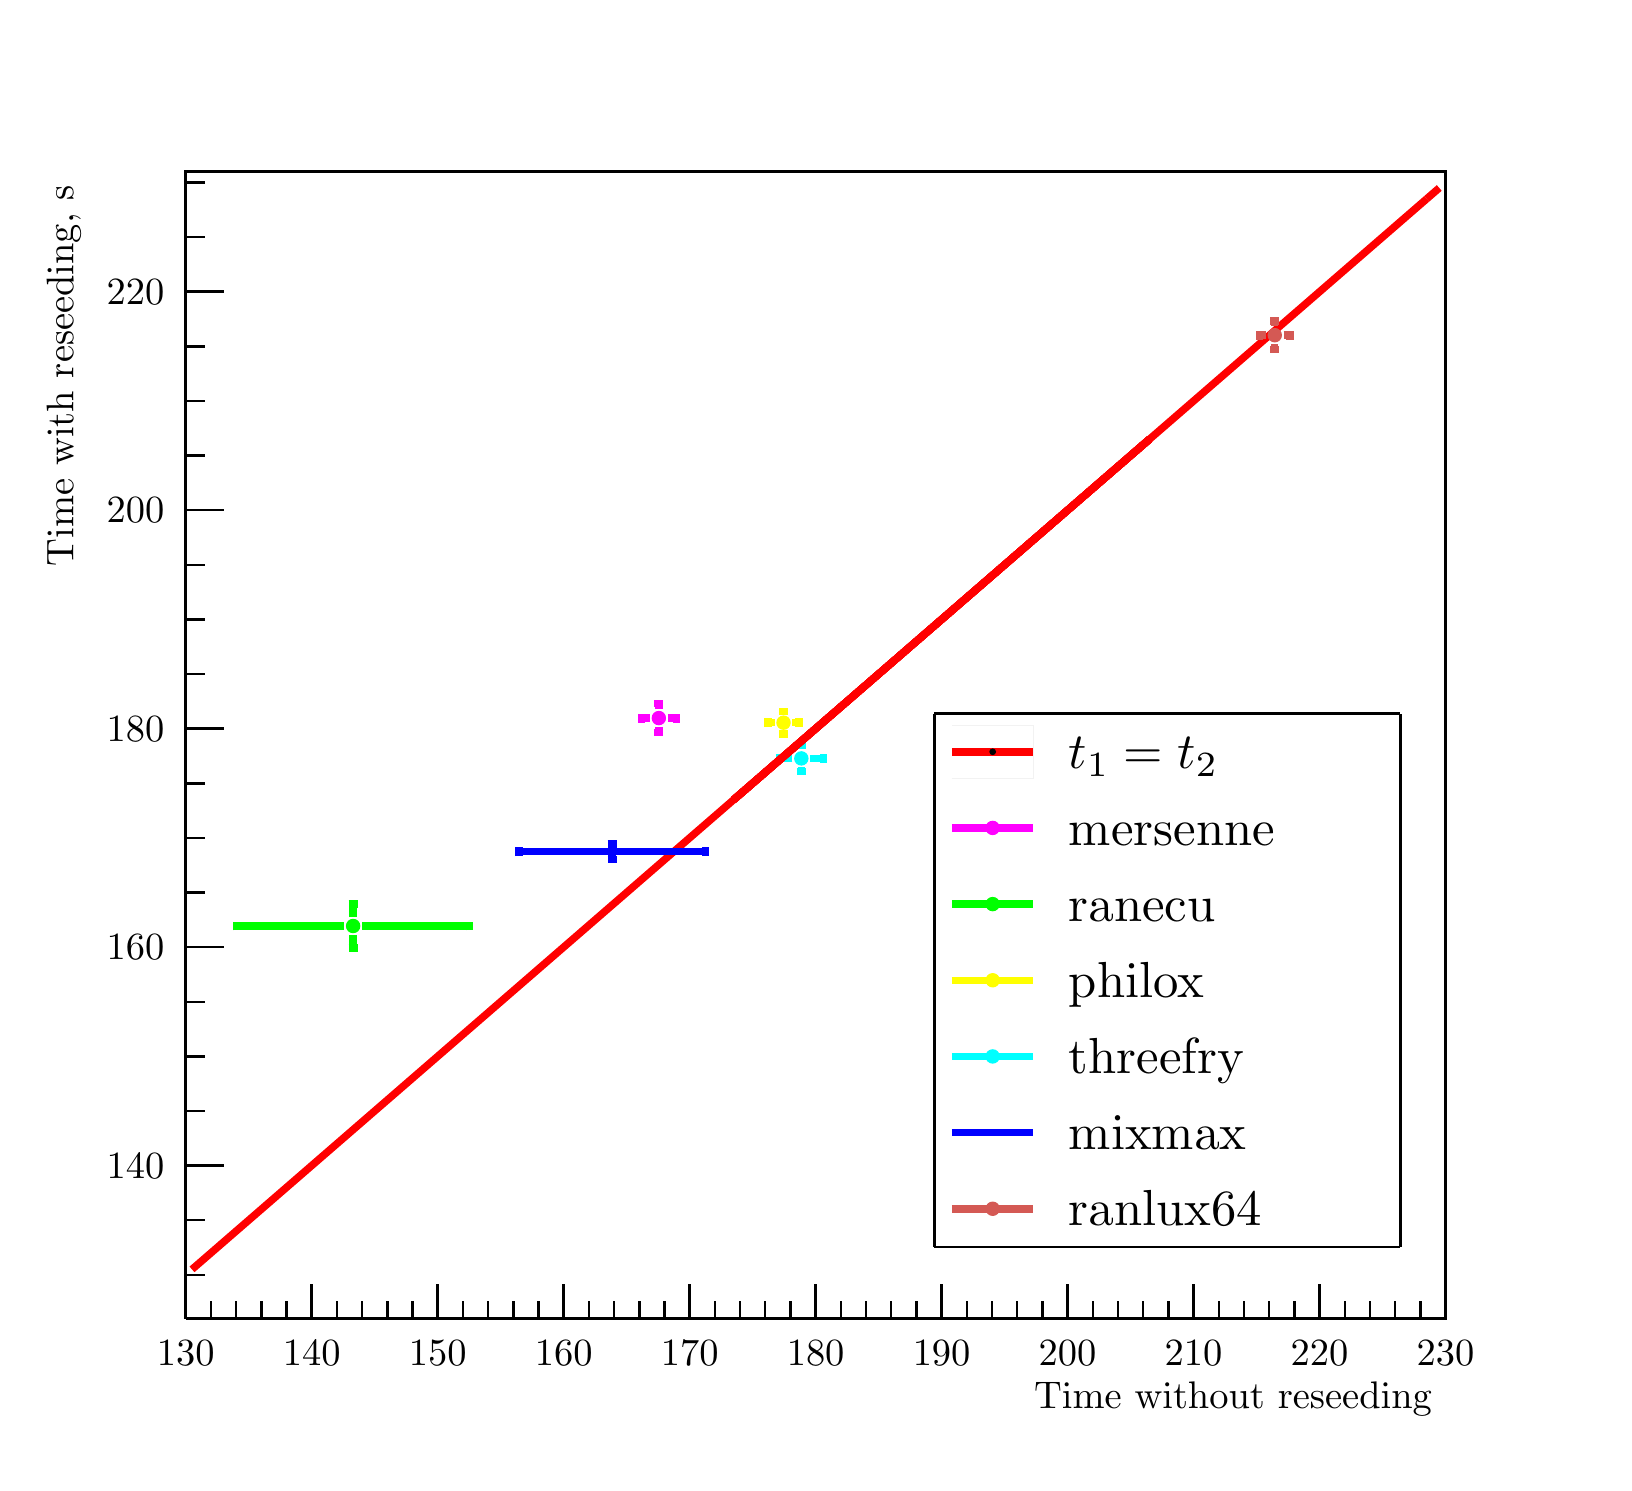
\begin{tikzpicture}
\pgfdeclareplotmark{cross} {
\pgfpathmoveto{\pgfpoint{-0.3\pgfplotmarksize}{\pgfplotmarksize}}
\pgfpathlineto{\pgfpoint{+0.3\pgfplotmarksize}{\pgfplotmarksize}}
\pgfpathlineto{\pgfpoint{+0.3\pgfplotmarksize}{0.3\pgfplotmarksize}}
\pgfpathlineto{\pgfpoint{+1\pgfplotmarksize}{0.3\pgfplotmarksize}}
\pgfpathlineto{\pgfpoint{+1\pgfplotmarksize}{-0.3\pgfplotmarksize}}
\pgfpathlineto{\pgfpoint{+0.3\pgfplotmarksize}{-0.3\pgfplotmarksize}}
\pgfpathlineto{\pgfpoint{+0.3\pgfplotmarksize}{-1.\pgfplotmarksize}}
\pgfpathlineto{\pgfpoint{-0.3\pgfplotmarksize}{-1.\pgfplotmarksize}}
\pgfpathlineto{\pgfpoint{-0.3\pgfplotmarksize}{-0.3\pgfplotmarksize}}
\pgfpathlineto{\pgfpoint{-1.\pgfplotmarksize}{-0.3\pgfplotmarksize}}
\pgfpathlineto{\pgfpoint{-1.\pgfplotmarksize}{0.3\pgfplotmarksize}}
\pgfpathlineto{\pgfpoint{-0.3\pgfplotmarksize}{0.3\pgfplotmarksize}}
\pgfpathclose
\pgfusepathqstroke
}
\pgfdeclareplotmark{cross*} {
\pgfpathmoveto{\pgfpoint{-0.3\pgfplotmarksize}{\pgfplotmarksize}}
\pgfpathlineto{\pgfpoint{+0.3\pgfplotmarksize}{\pgfplotmarksize}}
\pgfpathlineto{\pgfpoint{+0.3\pgfplotmarksize}{0.3\pgfplotmarksize}}
\pgfpathlineto{\pgfpoint{+1\pgfplotmarksize}{0.3\pgfplotmarksize}}
\pgfpathlineto{\pgfpoint{+1\pgfplotmarksize}{-0.3\pgfplotmarksize}}
\pgfpathlineto{\pgfpoint{+0.3\pgfplotmarksize}{-0.3\pgfplotmarksize}}
\pgfpathlineto{\pgfpoint{+0.3\pgfplotmarksize}{-1.\pgfplotmarksize}}
\pgfpathlineto{\pgfpoint{-0.3\pgfplotmarksize}{-1.\pgfplotmarksize}}
\pgfpathlineto{\pgfpoint{-0.3\pgfplotmarksize}{-0.3\pgfplotmarksize}}
\pgfpathlineto{\pgfpoint{-1.\pgfplotmarksize}{-0.3\pgfplotmarksize}}
\pgfpathlineto{\pgfpoint{-1.\pgfplotmarksize}{0.3\pgfplotmarksize}}
\pgfpathlineto{\pgfpoint{-0.3\pgfplotmarksize}{0.3\pgfplotmarksize}}
\pgfpathclose
\pgfusepathqfillstroke
}
\pgfdeclareplotmark{newstar} {
\pgfpathmoveto{\pgfqpoint{0pt}{\pgfplotmarksize}}
\pgfpathlineto{\pgfqpointpolar{44}{0.5\pgfplotmarksize}}
\pgfpathlineto{\pgfqpointpolar{18}{\pgfplotmarksize}}
\pgfpathlineto{\pgfqpointpolar{-20}{0.5\pgfplotmarksize}}
\pgfpathlineto{\pgfqpointpolar{-54}{\pgfplotmarksize}}
\pgfpathlineto{\pgfqpointpolar{-90}{0.5\pgfplotmarksize}}
\pgfpathlineto{\pgfqpointpolar{234}{\pgfplotmarksize}}
\pgfpathlineto{\pgfqpointpolar{198}{0.5\pgfplotmarksize}}
\pgfpathlineto{\pgfqpointpolar{162}{\pgfplotmarksize}}
\pgfpathlineto{\pgfqpointpolar{134}{0.5\pgfplotmarksize}}
\pgfpathclose
\pgfusepathqstroke
}
\pgfdeclareplotmark{newstar*} {
\pgfpathmoveto{\pgfqpoint{0pt}{\pgfplotmarksize}}
\pgfpathlineto{\pgfqpointpolar{44}{0.5\pgfplotmarksize}}
\pgfpathlineto{\pgfqpointpolar{18}{\pgfplotmarksize}}
\pgfpathlineto{\pgfqpointpolar{-20}{0.5\pgfplotmarksize}}
\pgfpathlineto{\pgfqpointpolar{-54}{\pgfplotmarksize}}
\pgfpathlineto{\pgfqpointpolar{-90}{0.5\pgfplotmarksize}}
\pgfpathlineto{\pgfqpointpolar{234}{\pgfplotmarksize}}
\pgfpathlineto{\pgfqpointpolar{198}{0.5\pgfplotmarksize}}
\pgfpathlineto{\pgfqpointpolar{162}{\pgfplotmarksize}}
\pgfpathlineto{\pgfqpointpolar{134}{0.5\pgfplotmarksize}}
\pgfpathclose
\pgfusepathqfillstroke
}
\definecolor{c}{rgb}{1,1,1};
\draw [color=c, fill=c] (0,0) rectangle (20,18.2077);
\draw [color=c, fill=c] (2,1.82077) rectangle (18,16.3869);
\definecolor{c}{rgb}{0,0,0};
\draw [c,line width=0.9] (2,1.82077) -- (2,16.3869) -- (18,16.3869) -- (18,1.82077) -- (2,1.82077);
\definecolor{c}{rgb}{1,1,1};
\draw [color=c, fill=c] (2,1.82077) rectangle (18,16.3869);
\definecolor{c}{rgb}{0,0,0};
\draw [c,line width=0.9] (2,1.82077) -- (2,16.3869) -- (18,16.3869) -- (18,1.82077) -- (2,1.82077);
\definecolor{c}{rgb}{1,0,0};
\draw [c,line width=2.7] (2.08,2.44503) -- (2.24,2.58376) -- (2.4,2.72248) -- (2.56,2.86121) -- (2.72,2.99993) -- (2.88,3.13866) -- (3.04,3.27738) -- (3.2,3.41611) -- (3.36,3.55483) -- (3.52,3.69356) -- (3.68,3.83228) -- (3.84,3.97101) -- (4,4.10973)
 -- (4.16,4.24846) -- (4.32,4.38718) -- (4.48,4.52591) -- (4.64,4.66463) -- (4.8,4.80336) -- (4.96,4.94209) -- (5.12,5.08081) -- (5.28,5.21954) -- (5.44,5.35826) -- (5.6,5.49699) -- (5.76,5.63571) -- (5.92,5.77444) -- (6.08,5.91316) -- (6.24,6.05189)
 -- (6.4,6.19061) -- (6.56,6.32934) -- (6.72,6.46806) -- (6.88,6.60679) -- (7.04,6.74551) -- (7.2,6.88424) -- (7.36,7.02296) -- (7.52,7.16169) -- (7.68,7.30041) -- (7.84,7.43914) -- (8,7.57786) -- (8.16,7.71659) -- (8.32,7.85531) -- (8.48,7.99404) --
 (8.64,8.13276) -- (8.8,8.27149) -- (8.96,8.41021) -- (9.12,8.54894) -- (9.28,8.68766) -- (9.44,8.82639) -- (9.6,8.96512) -- (9.76,9.10384) -- (9.92,9.24257);
\draw [c,line width=2.7] (9.92,9.24257) -- (10.08,9.38129) -- (10.24,9.52002) -- (10.4,9.65874) -- (10.56,9.79747) -- (10.72,9.93619) -- (10.88,10.0749) -- (11.04,10.2136) -- (11.2,10.3524) -- (11.36,10.4911) -- (11.52,10.6298) -- (11.68,10.7685) --
 (11.84,10.9073) -- (12,11.046) -- (12.16,11.1847) -- (12.32,11.3234) -- (12.48,11.4622) -- (12.64,11.6009) -- (12.8,11.7396) -- (12.96,11.8783) -- (13.12,12.0171) -- (13.28,12.1558) -- (13.44,12.2945) -- (13.6,12.4332) -- (13.76,12.572) --
 (13.92,12.7107) -- (14.08,12.8494) -- (14.24,12.9881) -- (14.4,13.1269) -- (14.56,13.2656) -- (14.72,13.4043) -- (14.88,13.543) -- (15.04,13.6818) -- (15.2,13.8205) -- (15.36,13.9592) -- (15.52,14.0979) -- (15.68,14.2367) -- (15.84,14.3754) --
 (16,14.5141) -- (16.16,14.6528) -- (16.32,14.7916) -- (16.48,14.9303) -- (16.64,15.069) -- (16.8,15.2077) -- (16.96,15.3465) -- (17.12,15.4852) -- (17.28,15.6239) -- (17.44,15.7627) -- (17.6,15.9014) -- (17.76,16.0401);
\draw [c,line width=2.7] (17.76,16.0401) -- (17.92,16.1788);
\definecolor{c}{rgb}{0,0,0};
\draw [c,line width=0.9] (2,1.82077) -- (18,1.82077);
\draw [c,line width=0.9] (2,2.25775) -- (2,1.82077);
\draw [c,line width=0.9] (2.32,2.03926) -- (2.32,1.82077);
\draw [c,line width=0.9] (2.64,2.03926) -- (2.64,1.82077);
\draw [c,line width=0.9] (2.96,2.03926) -- (2.96,1.82077);
\draw [c,line width=0.9] (3.28,2.03926) -- (3.28,1.82077);
\draw [c,line width=0.9] (3.6,2.25775) -- (3.6,1.82077);
\draw [c,line width=0.9] (3.92,2.03926) -- (3.92,1.82077);
\draw [c,line width=0.9] (4.24,2.03926) -- (4.24,1.82077);
\draw [c,line width=0.9] (4.56,2.03926) -- (4.56,1.82077);
\draw [c,line width=0.9] (4.88,2.03926) -- (4.88,1.82077);
\draw [c,line width=0.9] (5.2,2.25775) -- (5.2,1.82077);
\draw [c,line width=0.9] (5.52,2.03926) -- (5.52,1.82077);
\draw [c,line width=0.9] (5.84,2.03926) -- (5.84,1.82077);
\draw [c,line width=0.9] (6.16,2.03926) -- (6.16,1.82077);
\draw [c,line width=0.9] (6.48,2.03926) -- (6.48,1.82077);
\draw [c,line width=0.9] (6.8,2.25775) -- (6.8,1.82077);
\draw [c,line width=0.9] (7.12,2.03926) -- (7.12,1.82077);
\draw [c,line width=0.9] (7.44,2.03926) -- (7.44,1.82077);
\draw [c,line width=0.9] (7.76,2.03926) -- (7.76,1.82077);
\draw [c,line width=0.9] (8.08,2.03926) -- (8.08,1.82077);
\draw [c,line width=0.9] (8.4,2.25775) -- (8.4,1.82077);
\draw [c,line width=0.9] (8.72,2.03926) -- (8.72,1.82077);
\draw [c,line width=0.9] (9.04,2.03926) -- (9.04,1.82077);
\draw [c,line width=0.9] (9.36,2.03926) -- (9.36,1.82077);
\draw [c,line width=0.9] (9.68,2.03926) -- (9.68,1.82077);
\draw [c,line width=0.9] (10,2.25775) -- (10,1.82077);
\draw [c,line width=0.9] (10.32,2.03926) -- (10.32,1.82077);
\draw [c,line width=0.9] (10.64,2.03926) -- (10.64,1.82077);
\draw [c,line width=0.9] (10.96,2.03926) -- (10.96,1.82077);
\draw [c,line width=0.9] (11.28,2.03926) -- (11.28,1.82077);
\draw [c,line width=0.9] (11.6,2.25775) -- (11.6,1.82077);
\draw [c,line width=0.9] (11.92,2.03926) -- (11.92,1.82077);
\draw [c,line width=0.9] (12.24,2.03926) -- (12.24,1.82077);
\draw [c,line width=0.9] (12.56,2.03926) -- (12.56,1.82077);
\draw [c,line width=0.9] (12.88,2.03926) -- (12.88,1.82077);
\draw [c,line width=0.9] (13.2,2.25775) -- (13.2,1.82077);
\draw [c,line width=0.9] (13.52,2.03926) -- (13.52,1.82077);
\draw [c,line width=0.9] (13.84,2.03926) -- (13.84,1.82077);
\draw [c,line width=0.9] (14.16,2.03926) -- (14.16,1.82077);
\draw [c,line width=0.9] (14.48,2.03926) -- (14.48,1.82077);
\draw [c,line width=0.9] (14.8,2.25775) -- (14.8,1.82077);
\draw [c,line width=0.9] (15.12,2.03926) -- (15.12,1.82077);
\draw [c,line width=0.9] (15.44,2.03926) -- (15.44,1.82077);
\draw [c,line width=0.9] (15.76,2.03926) -- (15.76,1.82077);
\draw [c,line width=0.9] (16.08,2.03926) -- (16.08,1.82077);
\draw [c,line width=0.9] (16.4,2.25775) -- (16.4,1.82077);
\draw [c,line width=0.9] (16.72,2.03926) -- (16.72,1.82077);
\draw [c,line width=0.9] (17.04,2.03926) -- (17.04,1.82077);
\draw [c,line width=0.9] (17.36,2.03926) -- (17.36,1.82077);
\draw [c,line width=0.9] (17.68,2.03926) -- (17.68,1.82077);
\draw [c,line width=0.9] (18,2.25775) -- (18,1.82077);
\draw [anchor=base] (2,1.21991) node[scale=1.39008, color=c, rotate=0]{130};
\draw [anchor=base] (3.6,1.21991) node[scale=1.39008, color=c, rotate=0]{140};
\draw [anchor=base] (5.2,1.21991) node[scale=1.39008, color=c, rotate=0]{150};
\draw [anchor=base] (6.8,1.21991) node[scale=1.39008, color=c, rotate=0]{160};
\draw [anchor=base] (8.4,1.21991) node[scale=1.39008, color=c, rotate=0]{170};
\draw [anchor=base] (10,1.21991) node[scale=1.39008, color=c, rotate=0]{180};
\draw [anchor=base] (11.6,1.21991) node[scale=1.39008, color=c, rotate=0]{190};
\draw [anchor=base] (13.2,1.21991) node[scale=1.39008, color=c, rotate=0]{200};
\draw [anchor=base] (14.8,1.21991) node[scale=1.39008, color=c, rotate=0]{210};
\draw [anchor=base] (16.4,1.21991) node[scale=1.39008, color=c, rotate=0]{220};
\draw [anchor=base] (18,1.21991) node[scale=1.39008, color=c, rotate=0]{230};
\draw [anchor= east] (18,0.801138) node[scale=1.39008, color=c, rotate=0]{Time without reseeding};
\draw [c,line width=0.9] (2,1.82077) -- (2,16.3869);
\draw [c,line width=0.9] (2.48,3.76292) -- (2,3.76292);
\draw [c,line width=0.9] (2.24,4.45655) -- (2,4.45655);
\draw [c,line width=0.9] (2.24,5.15017) -- (2,5.15017);
\draw [c,line width=0.9] (2.24,5.8438) -- (2,5.8438);
\draw [c,line width=0.9] (2.48,6.53742) -- (2,6.53742);
\draw [c,line width=0.9] (2.24,7.23105) -- (2,7.23105);
\draw [c,line width=0.9] (2.24,7.92468) -- (2,7.92468);
\draw [c,line width=0.9] (2.24,8.6183) -- (2,8.6183);
\draw [c,line width=0.9] (2.48,9.31193) -- (2,9.31193);
\draw [c,line width=0.9] (2.24,10.0056) -- (2,10.0056);
\draw [c,line width=0.9] (2.24,10.6992) -- (2,10.6992);
\draw [c,line width=0.9] (2.24,11.3928) -- (2,11.3928);
\draw [c,line width=0.9] (2.48,12.0864) -- (2,12.0864);
\draw [c,line width=0.9] (2.24,12.7801) -- (2,12.7801);
\draw [c,line width=0.9] (2.24,13.4737) -- (2,13.4737);
\draw [c,line width=0.9] (2.24,14.1673) -- (2,14.1673);
\draw [c,line width=0.9] (2.48,14.8609) -- (2,14.8609);
\draw [c,line width=0.9] (2.48,3.76292) -- (2,3.76292);
\draw [c,line width=0.9] (2.24,3.06929) -- (2,3.06929);
\draw [c,line width=0.9] (2.24,2.37567) -- (2,2.37567);
\draw [c,line width=0.9] (2.48,14.8609) -- (2,14.8609);
\draw [c,line width=0.9] (2.24,15.5546) -- (2,15.5546);
\draw [c,line width=0.9] (2.24,16.2482) -- (2,16.2482);
\draw [anchor= east] (1.9,3.76292) node[scale=1.39008, color=c, rotate=0]{140};
\draw [anchor= east] (1.9,6.53742) node[scale=1.39008, color=c, rotate=0]{160};
\draw [anchor= east] (1.9,9.31193) node[scale=1.39008, color=c, rotate=0]{180};
\draw [anchor= east] (1.9,12.0864) node[scale=1.39008, color=c, rotate=0]{200};
\draw [anchor= east] (1.9,14.8609) node[scale=1.39008, color=c, rotate=0]{220};
\draw [anchor= east] (0.452347,16.3869) node[scale=1.39008, color=c, rotate=90]{Time with reseeding, s};
\definecolor{c}{rgb}{1,0,1};
\draw [c,line width=2.7] (7.895,9.44658) -- (7.7853,9.44658);
\draw [c,line width=2.7] (7.7853,9.38968) -- (7.7853,9.50348);
\draw [c,line width=2.7] (8.1226,9.44658) -- (8.2323,9.44658);
\draw [c,line width=2.7] (8.2323,9.38968) -- (8.2323,9.50348);
\draw [c,line width=2.7] (8.0088,9.56038) -- (8.0088,9.63112);
\draw [c,line width=2.7] (7.9519,9.63112) -- (8.0657,9.63112);
\draw [c,line width=2.7] (8.0088,9.33278) -- (8.0088,9.26204);
\draw [c,line width=2.7] (7.9519,9.26204) -- (8.0657,9.26204);
\foreach \P in {(8.0088,9.44658)}{\draw[mark options={color=c,fill=c},mark size=2.402402pt,mark=*] plot coordinates {\P};}
\definecolor{c}{rgb}{0,1,0};
\draw [c,line width=2.7] (4.0123,6.80586) -- (2.64491,6.80586);
\draw [c,line width=2.7] (2.64491,6.74896) -- (2.64491,6.86276);
\draw [c,line width=2.7] (4.2399,6.80586) -- (5.60729,6.80586);
\draw [c,line width=2.7] (5.60729,6.74896) -- (5.60729,6.86276);
\draw [c,line width=2.7] (4.1261,6.91966) -- (4.1261,7.08758);
\draw [c,line width=2.7] (4.0692,7.08758) -- (4.183,7.08758);
\draw [c,line width=2.7] (4.1261,6.69206) -- (4.1261,6.52414);
\draw [c,line width=2.7] (4.0692,6.52414) -- (4.183,6.52414);
\foreach \P in {(4.1261,6.80586)}{\draw[mark options={color=c,fill=c},mark size=2.402402pt,mark=*] plot coordinates {\P};}
\definecolor{c}{rgb}{1,1,0};
\draw [c,line width=2.7] (9.4785,9.38823) -- (9.3968,9.38823);
\draw [c,line width=2.7] (9.3968,9.33133) -- (9.3968,9.44513);
\draw [c,line width=2.7] (9.7061,9.38823) -- (9.7878,9.38823);
\draw [c,line width=2.7] (9.7878,9.33133) -- (9.7878,9.44513);
\draw [c,line width=2.7] (9.5923,9.50203) -- (9.5923,9.53051);
\draw [c,line width=2.7] (9.5354,9.53051) -- (9.6492,9.53051);
\draw [c,line width=2.7] (9.5923,9.27443) -- (9.5923,9.24595);
\draw [c,line width=2.7] (9.5354,9.24595) -- (9.6492,9.24595);
\foreach \P in {(9.5923,9.38823)}{\draw[mark options={color=c,fill=c},mark size=2.402402pt,mark=*] plot coordinates {\P};}
\definecolor{c}{rgb}{0,1,1};
\draw [c,line width=2.7] (9.7045,8.93434) -- (9.53897,8.93434);
\draw [c,line width=2.7] (9.53897,8.87744) -- (9.53897,8.99123);
\draw [c,line width=2.7] (9.9321,8.93434) -- (10.0976,8.93434);
\draw [c,line width=2.7] (10.0976,8.87744) -- (10.0976,8.99123);
\draw [c,line width=2.7] (9.8183,9.04813) -- (9.8183,9.09913);
\draw [c,line width=2.7] (9.7614,9.09913) -- (9.8752,9.09913);
\draw [c,line width=2.7] (9.8183,8.82054) -- (9.8183,8.76955);
\draw [c,line width=2.7] (9.7614,8.76955) -- (9.8752,8.76955);
\foreach \P in {(9.8183,8.93434)}{\draw[mark options={color=c,fill=c},mark size=2.402402pt,mark=*] plot coordinates {\P};}
\definecolor{c}{rgb}{0,0,1};
\draw [c,line width=2.7] (7.4154,7.74919) -- (6.23044,7.74919);
\draw [c,line width=2.7] (6.23044,7.69229) -- (6.23044,7.80609);
\draw [c,line width=2.7] (7.4154,7.74919) -- (8.60036,7.74919);
\draw [c,line width=2.7] (8.60036,7.69229) -- (8.60036,7.80609);
\draw [c,line width=2.7] (7.4154,7.74919) -- (7.4154,7.84836);
\draw [c,line width=2.7] (7.3585,7.84836) -- (7.4723,7.84836);
\draw [c,line width=2.7] (7.4154,7.74919) -- (7.4154,7.65002);
\draw [c,line width=2.7] (7.3585,7.65002) -- (7.4723,7.65002);
\foreach \P in {(7.4154,7.74919)}{\draw[mark options={color=c,fill=c},mark size=2.402402pt,mark=] plot coordinates {\P};}
\definecolor{c}{rgb}{0.83,0.35,0.33};
\draw [c,line width=2.7] (15.717,14.3089) -- (15.6367,14.3089);
\draw [c,line width=2.7] (15.6367,14.252) -- (15.6367,14.3658);
\draw [c,line width=2.7] (15.9446,14.3089) -- (16.0249,14.3089);
\draw [c,line width=2.7] (16.0249,14.252) -- (16.0249,14.3658);
\draw [c,line width=2.7] (15.8308,14.4227) -- (15.8308,14.4883);
\draw [c,line width=2.7] (15.7739,14.4883) -- (15.8877,14.4883);
\draw [c,line width=2.7] (15.8308,14.1951) -- (15.8308,14.1295);
\draw [c,line width=2.7] (15.7739,14.1295) -- (15.8877,14.1295);
\foreach \P in {(15.8308,14.3089)}{\draw[mark options={color=c,fill=c},mark size=2.402402pt,mark=*] plot coordinates {\P};}
\definecolor{c}{rgb}{1,1,1};
\draw [color=c, fill=c] (11.5089,2.73115) rectangle (17.426,9.50213);
\definecolor{c}{rgb}{0,0,0};
\draw [c,line width=0.9] (11.5089,2.73115) -- (17.426,2.73115);
\draw [c,line width=0.9] (17.426,2.73115) -- (17.426,9.50213);
\draw [c,line width=0.9] (17.426,9.50213) -- (11.5089,9.50213);
\draw [c,line width=0.9] (11.5089,9.50213) -- (11.5089,2.73115);
\draw [anchor=base west] (12.9882,8.80085) node[scale=1.83238, color=c, rotate=0]{$t_{1} = t_{2}$};
\definecolor{c}{rgb}{0.95,0.95,0.95};
\draw [c] (11.7308,8.67994) -- (12.7663,8.67994) -- (12.7663,9.35704) -- (11.7308,9.35704);
\definecolor{c}{rgb}{1,0,0};
\draw [c,line width=2.7] (11.7308,9.01849) -- (12.7663,9.01849);
\definecolor{c}{rgb}{0,0,0};
\foreach \P in {(12.2485,9.01849)}{\draw[mark options={color=c,fill=c},mark size=2.402402pt,mark=*,mark size=1pt] plot coordinates {\P};}
\draw [anchor=base west] (12.9882,7.83357) node[scale=1.83238, color=c, rotate=0]{mersenne};
\definecolor{c}{rgb}{1,1,1};
\draw [c] (11.7308,7.71266) -- (12.7663,7.71266) -- (12.7663,8.38976) -- (11.7308,8.38976);
\definecolor{c}{rgb}{1,0,1};
\draw [c,line width=2.7] (11.7308,8.05121) -- (12.7663,8.05121);
\foreach \P in {(12.2485,8.05121)}{\draw[mark options={color=c,fill=c},mark size=2.402402pt,mark=*] plot coordinates {\P};}
\definecolor{c}{rgb}{0,0,0};
\draw [anchor=base west] (12.9882,6.86629) node[scale=1.83238, color=c, rotate=0]{ranecu};
\definecolor{c}{rgb}{1,1,1};
\draw [c] (11.7308,6.74538) -- (12.7663,6.74538) -- (12.7663,7.42248) -- (11.7308,7.42248);
\definecolor{c}{rgb}{0,1,0};
\draw [c,line width=2.7] (11.7308,7.08393) -- (12.7663,7.08393);
\foreach \P in {(12.2485,7.08393)}{\draw[mark options={color=c,fill=c},mark size=2.402402pt,mark=*] plot coordinates {\P};}
\definecolor{c}{rgb}{0,0,0};
\draw [anchor=base west] (12.9882,5.899) node[scale=1.83238, color=c, rotate=0]{philox};
\definecolor{c}{rgb}{1,1,1};
\draw [c] (11.7308,5.77809) -- (12.7663,5.77809) -- (12.7663,6.45519) -- (11.7308,6.45519);
\definecolor{c}{rgb}{1,1,0};
\draw [c,line width=2.7] (11.7308,6.11664) -- (12.7663,6.11664);
\foreach \P in {(12.2485,6.11664)}{\draw[mark options={color=c,fill=c},mark size=2.402402pt,mark=*] plot coordinates {\P};}
\definecolor{c}{rgb}{0,0,0};
\draw [anchor=base west] (12.9882,4.93172) node[scale=1.83238, color=c, rotate=0]{threefry};
\definecolor{c}{rgb}{1,1,1};
\draw [c] (11.7308,4.81081) -- (12.7663,4.81081) -- (12.7663,5.48791) -- (11.7308,5.48791);
\definecolor{c}{rgb}{0,1,1};
\draw [c,line width=2.7] (11.7308,5.14936) -- (12.7663,5.14936);
\foreach \P in {(12.2485,5.14936)}{\draw[mark options={color=c,fill=c},mark size=2.402402pt,mark=*] plot coordinates {\P};}
\definecolor{c}{rgb}{0,0,0};
\draw [anchor=base west] (12.9882,3.96444) node[scale=1.83238, color=c, rotate=0]{mixmax};
\definecolor{c}{rgb}{1,1,1};
\draw [c] (11.7308,3.84353) -- (12.7663,3.84353) -- (12.7663,4.52063) -- (11.7308,4.52063);
\definecolor{c}{rgb}{0,0,1};
\draw [c,line width=2.7] (11.7308,4.18208) -- (12.7663,4.18208);
\foreach \P in {(12.2485,4.18208)}{\draw[mark options={color=c,fill=c},mark size=2.402402pt,mark=] plot coordinates {\P};}
\definecolor{c}{rgb}{0,0,0};
\draw [anchor=base west] (12.9882,2.99716) node[scale=1.83238, color=c, rotate=0]{ranlux64};
\definecolor{c}{rgb}{1,1,1};
\draw [c] (11.7308,2.87624) -- (12.7663,2.87624) -- (12.7663,3.55334) -- (11.7308,3.55334);
\definecolor{c}{rgb}{0.83,0.35,0.33};
\draw [c,line width=2.7] (11.7308,3.21479) -- (12.7663,3.21479);
\foreach \P in {(12.2485,3.21479)}{\draw[mark options={color=c,fill=c},mark size=2.402402pt,mark=*] plot coordinates {\P};}
\definecolor{c}{rgb}{1,0,0};
\draw [c,line width=2.7] (8.96,8.41021) -- (9.01333,8.45646) -- (9.06667,8.5027) -- (9.12,8.54894) -- (9.17333,8.59518) -- (9.22667,8.64142) -- (9.28,8.68766) -- (9.33333,8.73391) -- (9.38667,8.78015) -- (9.44,8.82639) -- (9.49333,8.87263) --
 (9.54667,8.91887) -- (9.6,8.96512) -- (9.65333,9.01136) -- (9.70667,9.0576) -- (9.76,9.10384) -- (9.81333,9.15008) -- (9.86667,9.19632) -- (9.92,9.24257) -- (9.97333,9.28881) -- (10.0267,9.33505) -- (10.08,9.38129) -- (10.1333,9.42753) --
 (10.1867,9.47377) -- (10.24,9.52002) -- (10.2933,9.56626) -- (10.3467,9.6125) -- (10.4,9.65874) -- (10.4533,9.70498) -- (10.5067,9.75123) -- (10.56,9.79747) -- (10.6133,9.84371) -- (10.6667,9.88995) -- (10.72,9.93619) -- (10.7733,9.98243) --
 (10.8267,10.0287) -- (10.88,10.0749) -- (10.9333,10.1212) -- (10.9867,10.1674) -- (11.04,10.2136) -- (11.0933,10.2599) -- (11.1467,10.3061) -- (11.2,10.3524) -- (11.2533,10.3986) -- (11.3067,10.4449) -- (11.36,10.4911) -- (11.4133,10.5373) --
 (11.4667,10.5836) -- (11.52,10.6298) -- (11.5733,10.6761);
\draw [c,line width=2.7] (11.5733,10.6761) -- (11.6267,10.7223) -- (11.68,10.7685) -- (11.7333,10.8148) -- (11.7867,10.861) -- (11.84,10.9073) -- (11.8933,10.9535) -- (11.9467,10.9998) -- (12,11.046) -- (12.0533,11.0922) -- (12.1067,11.1385) --
 (12.16,11.1847) -- (12.2133,11.231) -- (12.2667,11.2772) -- (12.32,11.3234) -- (12.3733,11.3697) -- (12.4267,11.4159) -- (12.48,11.4622) -- (12.5333,11.5084) -- (12.5867,11.5547) -- (12.64,11.6009) -- (12.6933,11.6471) -- (12.7467,11.6934) --
 (12.8,11.7396) -- (12.8533,11.7859) -- (12.9067,11.8321) -- (12.96,11.8783) -- (13.0133,11.9246) -- (13.0667,11.9708) -- (13.12,12.0171) -- (13.1733,12.0633) -- (13.2267,12.1096) -- (13.28,12.1558) -- (13.3333,12.202) -- (13.3867,12.2483) --
 (13.44,12.2945) -- (13.4933,12.3408) -- (13.5467,12.387) -- (13.6,12.4332) -- (13.6533,12.4795) -- (13.7067,12.5257) -- (13.76,12.572) -- (13.8133,12.6182) -- (13.8667,12.6645) -- (13.92,12.7107) -- (13.9733,12.7569) -- (14.0267,12.8032) --
 (14.08,12.8494) -- (14.1333,12.8957) -- (14.1867,12.9419);
\draw [c,line width=2.7] (14.1867,12.9419) -- (14.24,12.9881);
\draw [c,line width=2.7] (8.96,8.41021) -- (9.01333,8.45646) -- (9.06667,8.5027) -- (9.12,8.54894) -- (9.17333,8.59518) -- (9.22667,8.64142) -- (9.28,8.68766) -- (9.33333,8.73391) -- (9.38667,8.78015) -- (9.44,8.82639) -- (9.49333,8.87263) --
 (9.54667,8.91887) -- (9.6,8.96512) -- (9.65333,9.01136) -- (9.70667,9.0576) -- (9.76,9.10384) -- (9.81333,9.15008) -- (9.86667,9.19632) -- (9.92,9.24257) -- (9.97333,9.28881) -- (10.0267,9.33505) -- (10.08,9.38129) -- (10.1333,9.42753) --
 (10.1867,9.47377) -- (10.24,9.52002) -- (10.2933,9.56626) -- (10.3467,9.6125) -- (10.4,9.65874) -- (10.4533,9.70498) -- (10.5067,9.75123) -- (10.56,9.79747) -- (10.6133,9.84371) -- (10.6667,9.88995) -- (10.72,9.93619) -- (10.7733,9.98243) --
 (10.8267,10.0287) -- (10.88,10.0749) -- (10.9333,10.1212) -- (10.9867,10.1674) -- (11.04,10.2136) -- (11.0933,10.2599) -- (11.1467,10.3061) -- (11.2,10.3524) -- (11.2533,10.3986) -- (11.3067,10.4449) -- (11.36,10.4911) -- (11.4133,10.5373) --
 (11.4667,10.5836) -- (11.52,10.6298) -- (11.5733,10.6761);
\draw [c,line width=2.7] (11.5733,10.6761) -- (11.6267,10.7223) -- (11.68,10.7685) -- (11.7333,10.8148) -- (11.7867,10.861) -- (11.84,10.9073) -- (11.8933,10.9535) -- (11.9467,10.9998) -- (12,11.046) -- (12.0533,11.0922) -- (12.1067,11.1385) --
 (12.16,11.1847) -- (12.2133,11.231) -- (12.2667,11.2772) -- (12.32,11.3234) -- (12.3733,11.3697) -- (12.4267,11.4159) -- (12.48,11.4622) -- (12.5333,11.5084) -- (12.5867,11.5547) -- (12.64,11.6009) -- (12.6933,11.6471) -- (12.7467,11.6934) --
 (12.8,11.7396) -- (12.8533,11.7859) -- (12.9067,11.8321) -- (12.96,11.8783) -- (13.0133,11.9246) -- (13.0667,11.9708) -- (13.12,12.0171) -- (13.1733,12.0633) -- (13.2267,12.1096) -- (13.28,12.1558) -- (13.3333,12.202) -- (13.3867,12.2483) --
 (13.44,12.2945) -- (13.4933,12.3408) -- (13.5467,12.387) -- (13.6,12.4332) -- (13.6533,12.4795) -- (13.7067,12.5257) -- (13.76,12.572) -- (13.8133,12.6182) -- (13.8667,12.6645) -- (13.92,12.7107) -- (13.9733,12.7569) -- (14.0267,12.8032) --
 (14.08,12.8494) -- (14.1333,12.8957) -- (14.1867,12.9419);
\draw [c,line width=2.7] (14.1867,12.9419) -- (14.24,12.9881);
\draw [c,line width=2.7] (8.96,8.41021) -- (9.01333,8.45646) -- (9.06667,8.5027) -- (9.12,8.54894) -- (9.17333,8.59518) -- (9.22667,8.64142) -- (9.28,8.68766) -- (9.33333,8.73391) -- (9.38667,8.78015) -- (9.44,8.82639) -- (9.49333,8.87263) --
 (9.54667,8.91887) -- (9.6,8.96512) -- (9.65333,9.01136) -- (9.70667,9.0576) -- (9.76,9.10384) -- (9.81333,9.15008) -- (9.86667,9.19632) -- (9.92,9.24257) -- (9.97333,9.28881) -- (10.0267,9.33505) -- (10.08,9.38129) -- (10.1333,9.42753) --
 (10.1867,9.47377) -- (10.24,9.52002) -- (10.2933,9.56626) -- (10.3467,9.6125) -- (10.4,9.65874) -- (10.4533,9.70498) -- (10.5067,9.75123) -- (10.56,9.79747) -- (10.6133,9.84371) -- (10.6667,9.88995) -- (10.72,9.93619) -- (10.7733,9.98243) --
 (10.8267,10.0287) -- (10.88,10.0749) -- (10.9333,10.1212) -- (10.9867,10.1674) -- (11.04,10.2136) -- (11.0933,10.2599) -- (11.1467,10.3061) -- (11.2,10.3524) -- (11.2533,10.3986) -- (11.3067,10.4449) -- (11.36,10.4911) -- (11.4133,10.5373) --
 (11.4667,10.5836) -- (11.52,10.6298) -- (11.5733,10.6761);
\draw [c,line width=2.7] (11.5733,10.6761) -- (11.6267,10.7223) -- (11.68,10.7685) -- (11.7333,10.8148) -- (11.7867,10.861) -- (11.84,10.9073) -- (11.8933,10.9535) -- (11.9467,10.9998) -- (12,11.046) -- (12.0533,11.0922) -- (12.1067,11.1385) --
 (12.16,11.1847) -- (12.2133,11.231) -- (12.2667,11.2772) -- (12.32,11.3234) -- (12.3733,11.3697) -- (12.4267,11.4159) -- (12.48,11.4622) -- (12.5333,11.5084) -- (12.5867,11.5547) -- (12.64,11.6009) -- (12.6933,11.6471) -- (12.7467,11.6934) --
 (12.8,11.7396) -- (12.8533,11.7859) -- (12.9067,11.8321) -- (12.96,11.8783) -- (13.0133,11.9246) -- (13.0667,11.9708) -- (13.12,12.0171) -- (13.1733,12.0633) -- (13.2267,12.1096) -- (13.28,12.1558) -- (13.3333,12.202) -- (13.3867,12.2483) --
 (13.44,12.2945) -- (13.4933,12.3408) -- (13.5467,12.387) -- (13.6,12.4332) -- (13.6533,12.4795) -- (13.7067,12.5257) -- (13.76,12.572) -- (13.8133,12.6182) -- (13.8667,12.6645) -- (13.92,12.7107) -- (13.9733,12.7569) -- (14.0267,12.8032) --
 (14.08,12.8494) -- (14.1333,12.8957) -- (14.1867,12.9419);
\draw [c,line width=2.7] (14.1867,12.9419) -- (14.24,12.9881);
\draw [c,line width=2.7] (8.96,8.41021) -- (9.01333,8.45646) -- (9.06667,8.5027) -- (9.12,8.54894) -- (9.17333,8.59518) -- (9.22667,8.64142) -- (9.28,8.68766) -- (9.33333,8.73391) -- (9.38667,8.78015) -- (9.44,8.82639) -- (9.49333,8.87263) --
 (9.54667,8.91887) -- (9.6,8.96512) -- (9.65333,9.01136) -- (9.70667,9.0576) -- (9.76,9.10384) -- (9.81333,9.15008) -- (9.86667,9.19632) -- (9.92,9.24257) -- (9.97333,9.28881) -- (10.0267,9.33505) -- (10.08,9.38129) -- (10.1333,9.42753) --
 (10.1867,9.47377) -- (10.24,9.52002) -- (10.2933,9.56626) -- (10.3467,9.6125) -- (10.4,9.65874) -- (10.4533,9.70498) -- (10.5067,9.75123) -- (10.56,9.79747) -- (10.6133,9.84371) -- (10.6667,9.88995) -- (10.72,9.93619) -- (10.7733,9.98243) --
 (10.8267,10.0287) -- (10.88,10.0749) -- (10.9333,10.1212) -- (10.9867,10.1674) -- (11.04,10.2136) -- (11.0933,10.2599) -- (11.1467,10.3061) -- (11.2,10.3524) -- (11.2533,10.3986) -- (11.3067,10.4449) -- (11.36,10.4911) -- (11.4133,10.5373) --
 (11.4667,10.5836) -- (11.52,10.6298) -- (11.5733,10.6761);
\draw [c,line width=2.7] (11.5733,10.6761) -- (11.6267,10.7223) -- (11.68,10.7685) -- (11.7333,10.8148) -- (11.7867,10.861) -- (11.84,10.9073) -- (11.8933,10.9535) -- (11.9467,10.9998) -- (12,11.046) -- (12.0533,11.0922) -- (12.1067,11.1385) --
 (12.16,11.1847) -- (12.2133,11.231) -- (12.2667,11.2772) -- (12.32,11.3234) -- (12.3733,11.3697) -- (12.4267,11.4159) -- (12.48,11.4622) -- (12.5333,11.5084) -- (12.5867,11.5547) -- (12.64,11.6009) -- (12.6933,11.6471) -- (12.7467,11.6934) --
 (12.8,11.7396) -- (12.8533,11.7859) -- (12.9067,11.8321) -- (12.96,11.8783) -- (13.0133,11.9246) -- (13.0667,11.9708) -- (13.12,12.0171) -- (13.1733,12.0633) -- (13.2267,12.1096) -- (13.28,12.1558) -- (13.3333,12.202) -- (13.3867,12.2483) --
 (13.44,12.2945) -- (13.4933,12.3408) -- (13.5467,12.387) -- (13.6,12.4332) -- (13.6533,12.4795) -- (13.7067,12.5257) -- (13.76,12.572) -- (13.8133,12.6182) -- (13.8667,12.6645) -- (13.92,12.7107) -- (13.9733,12.7569) -- (14.0267,12.8032) --
 (14.08,12.8494) -- (14.1333,12.8957) -- (14.1867,12.9419);
\draw [c,line width=2.7] (14.1867,12.9419) -- (14.24,12.9881);
\draw [c,line width=2.7] (8.96,8.41021) -- (9.01333,8.45646) -- (9.06667,8.5027) -- (9.12,8.54894) -- (9.17333,8.59518) -- (9.22667,8.64142) -- (9.28,8.68766) -- (9.33333,8.73391) -- (9.38667,8.78015) -- (9.44,8.82639) -- (9.49333,8.87263) --
 (9.54667,8.91887) -- (9.6,8.96512) -- (9.65333,9.01136) -- (9.70667,9.0576) -- (9.76,9.10384) -- (9.81333,9.15008) -- (9.86667,9.19632) -- (9.92,9.24257) -- (9.97333,9.28881) -- (10.0267,9.33505) -- (10.08,9.38129) -- (10.1333,9.42753) --
 (10.1867,9.47377) -- (10.24,9.52002) -- (10.2933,9.56626) -- (10.3467,9.6125) -- (10.4,9.65874) -- (10.4533,9.70498) -- (10.5067,9.75123) -- (10.56,9.79747) -- (10.6133,9.84371) -- (10.6667,9.88995) -- (10.72,9.93619) -- (10.7733,9.98243) --
 (10.8267,10.0287) -- (10.88,10.0749) -- (10.9333,10.1212) -- (10.9867,10.1674) -- (11.04,10.2136) -- (11.0933,10.2599) -- (11.1467,10.3061) -- (11.2,10.3524) -- (11.2533,10.3986) -- (11.3067,10.4449) -- (11.36,10.4911) -- (11.4133,10.5373) --
 (11.4667,10.5836) -- (11.52,10.6298) -- (11.5733,10.6761);
\draw [c,line width=2.7] (11.5733,10.6761) -- (11.6267,10.7223) -- (11.68,10.7685) -- (11.7333,10.8148) -- (11.7867,10.861) -- (11.84,10.9073) -- (11.8933,10.9535) -- (11.9467,10.9998) -- (12,11.046) -- (12.0533,11.0922) -- (12.1067,11.1385) --
 (12.16,11.1847) -- (12.2133,11.231) -- (12.2667,11.2772) -- (12.32,11.3234) -- (12.3733,11.3697) -- (12.4267,11.4159) -- (12.48,11.4622) -- (12.5333,11.5084) -- (12.5867,11.5547) -- (12.64,11.6009) -- (12.6933,11.6471) -- (12.7467,11.6934) --
 (12.8,11.7396) -- (12.8533,11.7859) -- (12.9067,11.8321) -- (12.96,11.8783) -- (13.0133,11.9246) -- (13.0667,11.9708) -- (13.12,12.0171) -- (13.1733,12.0633) -- (13.2267,12.1096) -- (13.28,12.1558) -- (13.3333,12.202) -- (13.3867,12.2483) --
 (13.44,12.2945) -- (13.4933,12.3408) -- (13.5467,12.387) -- (13.6,12.4332) -- (13.6533,12.4795) -- (13.7067,12.5257) -- (13.76,12.572) -- (13.8133,12.6182) -- (13.8667,12.6645) -- (13.92,12.7107) -- (13.9733,12.7569) -- (14.0267,12.8032) --
 (14.08,12.8494) -- (14.1333,12.8957) -- (14.1867,12.9419);
\draw [c,line width=2.7] (14.1867,12.9419) -- (14.24,12.9881);
\draw [c,line width=2.7] (8.96,8.41021) -- (9.01333,8.45646) -- (9.06667,8.5027) -- (9.12,8.54894) -- (9.17333,8.59518) -- (9.22667,8.64142) -- (9.28,8.68766) -- (9.33333,8.73391) -- (9.38667,8.78015) -- (9.44,8.82639) -- (9.49333,8.87263) --
 (9.54667,8.91887) -- (9.6,8.96512) -- (9.65333,9.01136) -- (9.70667,9.0576) -- (9.76,9.10384) -- (9.81333,9.15008) -- (9.86667,9.19632) -- (9.92,9.24257) -- (9.97333,9.28881) -- (10.0267,9.33505) -- (10.08,9.38129) -- (10.1333,9.42753) --
 (10.1867,9.47377) -- (10.24,9.52002) -- (10.2933,9.56626) -- (10.3467,9.6125) -- (10.4,9.65874) -- (10.4533,9.70498) -- (10.5067,9.75123) -- (10.56,9.79747) -- (10.6133,9.84371) -- (10.6667,9.88995) -- (10.72,9.93619) -- (10.7733,9.98243) --
 (10.8267,10.0287) -- (10.88,10.0749) -- (10.9333,10.1212) -- (10.9867,10.1674) -- (11.04,10.2136) -- (11.0933,10.2599) -- (11.1467,10.3061) -- (11.2,10.3524) -- (11.2533,10.3986) -- (11.3067,10.4449) -- (11.36,10.4911) -- (11.4133,10.5373) --
 (11.4667,10.5836) -- (11.52,10.6298) -- (11.5733,10.6761);
\draw [c,line width=2.7] (11.5733,10.6761) -- (11.6267,10.7223) -- (11.68,10.7685) -- (11.7333,10.8148) -- (11.7867,10.861) -- (11.84,10.9073) -- (11.8933,10.9535) -- (11.9467,10.9998) -- (12,11.046) -- (12.0533,11.0922) -- (12.1067,11.1385) --
 (12.16,11.1847) -- (12.2133,11.231) -- (12.2667,11.2772) -- (12.32,11.3234) -- (12.3733,11.3697) -- (12.4267,11.4159) -- (12.48,11.4622) -- (12.5333,11.5084) -- (12.5867,11.5547) -- (12.64,11.6009) -- (12.6933,11.6471) -- (12.7467,11.6934) --
 (12.8,11.7396) -- (12.8533,11.7859) -- (12.9067,11.8321) -- (12.96,11.8783) -- (13.0133,11.9246) -- (13.0667,11.9708) -- (13.12,12.0171) -- (13.1733,12.0633) -- (13.2267,12.1096) -- (13.28,12.1558) -- (13.3333,12.202) -- (13.3867,12.2483) --
 (13.44,12.2945) -- (13.4933,12.3408) -- (13.5467,12.387) -- (13.6,12.4332) -- (13.6533,12.4795) -- (13.7067,12.5257) -- (13.76,12.572) -- (13.8133,12.6182) -- (13.8667,12.6645) -- (13.92,12.7107) -- (13.9733,12.7569) -- (14.0267,12.8032) --
 (14.08,12.8494) -- (14.1333,12.8957) -- (14.1867,12.9419);
\draw [c,line width=2.7] (14.1867,12.9419) -- (14.24,12.9881);
\end{tikzpicture}
}
   \caption{User run time with (Y axis) and without (X axis) reseeding.}
  \end{figure}
 
 
 \section{Conclusion}
 
 \section{Acknowledgements}
  Development sponsored by Google in Google Summer of Code 2017 under supervision of John Apostolakis and Sandro Wenzel.
 
 \newpage
 \bibliographystyle{plain}
 \bibliography{gsocPreprint}
 
 \appendix
  \section{Test macros}
   \label{TESTMACROS}
   
   \VerbatimInput{runTr.mac}
   
   \VerbatimInput{runSomeTimes.mac}
  
  \section{Test results}
   \label{TESTRESULTS}
   \subsection{Reproducibility}
   
   \VerbatimInput{script.out}
   
   \subsection{Physical results}

    Debug build:\\
    \begin{tabular}{ l c c c c r }
     1 & 0.22 & 0.83 & 0.79 & 0.12 & 0.57 \\
     0.22 & 1 & 0.19 & 0.42 & 0.89 & 0.8 \\
     0.83 & 0.19 & 1 & 0.68 & 0.5 & 0.79 \\
     0.79 & 0.42 & 0.68 & 1 & 0.29 & 0.79 \\
     0.12 & 0.89 & 0.5 & 0.29 & 1 & 0.76 \\
     0.57 & 0.8 & 0.79 & 0.79 & 0.76 & 1 \\
    \end{tabular}
   
    Release build with 10x statistics:\\
    \begin{tabular}{ l c c c c r }
     1 & 0.44 & 0.07 & 0.39 & 0.12 & 0.5 \\
     0.44 & 1 & 0.52 & 0.97 & 0.79 & 0.93 \\
     0.07 & 0.52 & 1 & 0.33 & 0.2 & 0.56 \\
     0.39 & 0.97 & 0.33 & 1 & 0.85 & 0.83 \\
     0.12 & 0.79 & 0.2 & 0.85 & 1 & 0.42 \\
     0.5 & 0.93 & 0.56 & 0.83 & 0.42 & 1 \\
    \end{tabular}
    
    With reseeding activated:\\
    \begin{tabular}{ l c c c c r }
     1 & 0.91 & 0.6 & 0.33 & 0.26 & 0.35 \\
     0.91 & 1 & 0.02 & 0.85 & 0.82 & 0.5 \\
     0.6 & 0.02 & 1 & 0.1 & 0.26 & 0.76 \\
     0.33 & 0.85 & 0.1 & 1 & 0.84 & 0.57 \\
     0.26 & 0.82 & 0.26 & 0.84 & 1 & 0.68 \\
     0.35 & 0.5 & 0.76 & 0.57 & 0.68 & 1 \\
    \end{tabular}
    
   \subsection{Performance}
    
    \scalebox{.8}{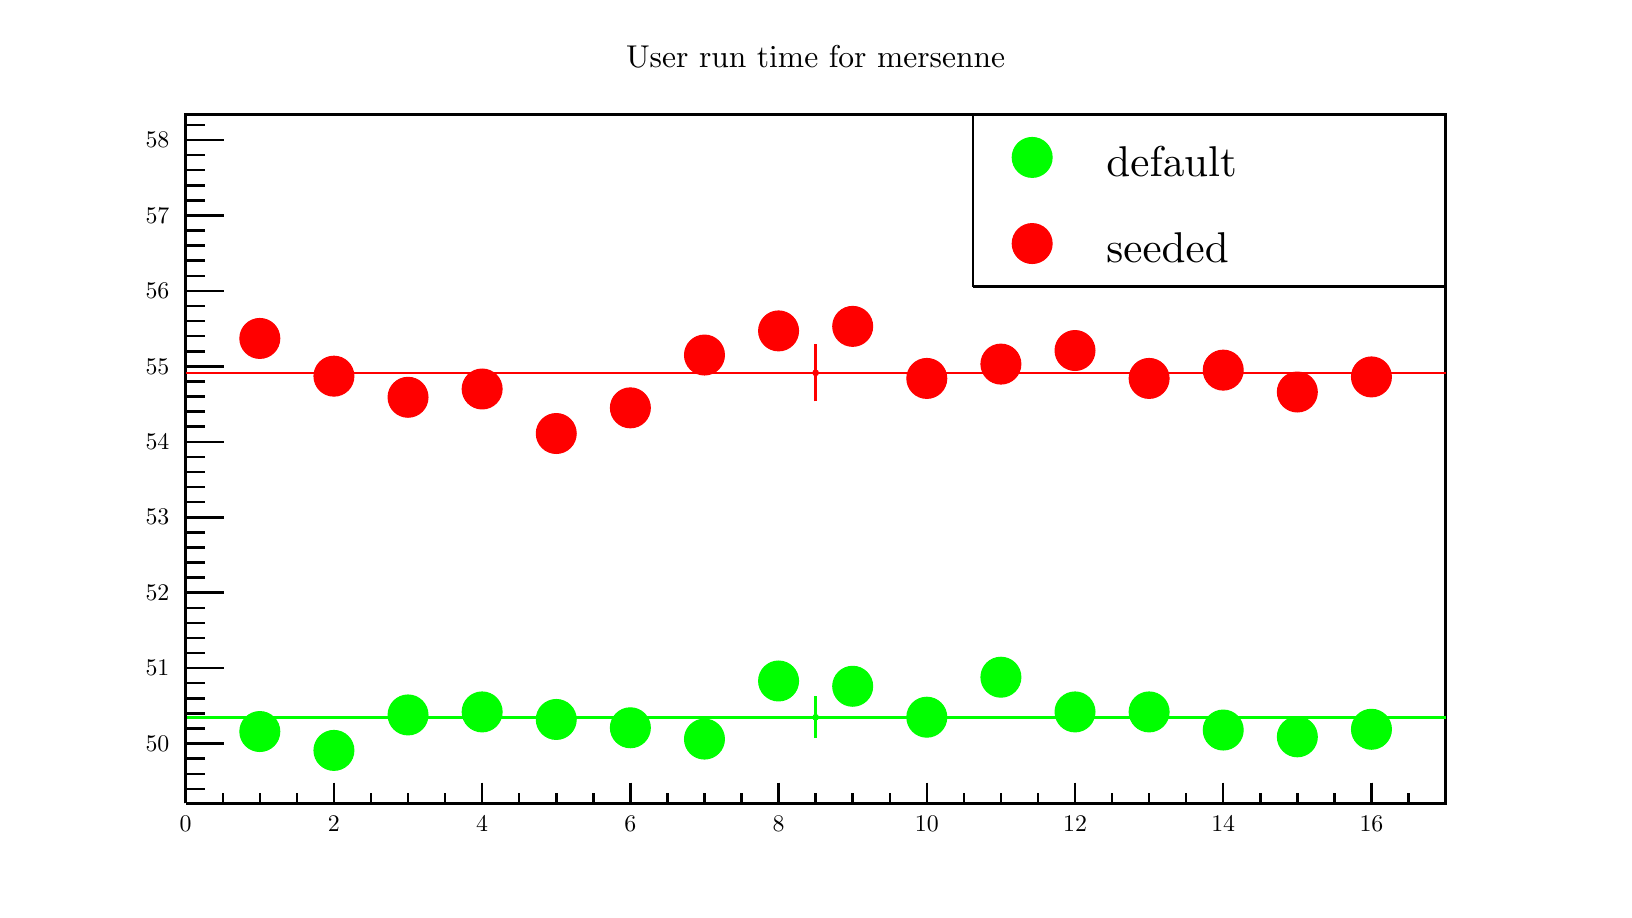
\begin{tikzpicture}
\pgfdeclareplotmark{cross} {
\pgfpathmoveto{\pgfpoint{-0.3\pgfplotmarksize}{\pgfplotmarksize}}
\pgfpathlineto{\pgfpoint{+0.3\pgfplotmarksize}{\pgfplotmarksize}}
\pgfpathlineto{\pgfpoint{+0.3\pgfplotmarksize}{0.3\pgfplotmarksize}}
\pgfpathlineto{\pgfpoint{+1\pgfplotmarksize}{0.3\pgfplotmarksize}}
\pgfpathlineto{\pgfpoint{+1\pgfplotmarksize}{-0.3\pgfplotmarksize}}
\pgfpathlineto{\pgfpoint{+0.3\pgfplotmarksize}{-0.3\pgfplotmarksize}}
\pgfpathlineto{\pgfpoint{+0.3\pgfplotmarksize}{-1.\pgfplotmarksize}}
\pgfpathlineto{\pgfpoint{-0.3\pgfplotmarksize}{-1.\pgfplotmarksize}}
\pgfpathlineto{\pgfpoint{-0.3\pgfplotmarksize}{-0.3\pgfplotmarksize}}
\pgfpathlineto{\pgfpoint{-1.\pgfplotmarksize}{-0.3\pgfplotmarksize}}
\pgfpathlineto{\pgfpoint{-1.\pgfplotmarksize}{0.3\pgfplotmarksize}}
\pgfpathlineto{\pgfpoint{-0.3\pgfplotmarksize}{0.3\pgfplotmarksize}}
\pgfpathclose
\pgfusepathqstroke
}
\pgfdeclareplotmark{cross*} {
\pgfpathmoveto{\pgfpoint{-0.3\pgfplotmarksize}{\pgfplotmarksize}}
\pgfpathlineto{\pgfpoint{+0.3\pgfplotmarksize}{\pgfplotmarksize}}
\pgfpathlineto{\pgfpoint{+0.3\pgfplotmarksize}{0.3\pgfplotmarksize}}
\pgfpathlineto{\pgfpoint{+1\pgfplotmarksize}{0.3\pgfplotmarksize}}
\pgfpathlineto{\pgfpoint{+1\pgfplotmarksize}{-0.3\pgfplotmarksize}}
\pgfpathlineto{\pgfpoint{+0.3\pgfplotmarksize}{-0.3\pgfplotmarksize}}
\pgfpathlineto{\pgfpoint{+0.3\pgfplotmarksize}{-1.\pgfplotmarksize}}
\pgfpathlineto{\pgfpoint{-0.3\pgfplotmarksize}{-1.\pgfplotmarksize}}
\pgfpathlineto{\pgfpoint{-0.3\pgfplotmarksize}{-0.3\pgfplotmarksize}}
\pgfpathlineto{\pgfpoint{-1.\pgfplotmarksize}{-0.3\pgfplotmarksize}}
\pgfpathlineto{\pgfpoint{-1.\pgfplotmarksize}{0.3\pgfplotmarksize}}
\pgfpathlineto{\pgfpoint{-0.3\pgfplotmarksize}{0.3\pgfplotmarksize}}
\pgfpathclose
\pgfusepathqfillstroke
}
\pgfdeclareplotmark{newstar} {
\pgfpathmoveto{\pgfqpoint{0pt}{\pgfplotmarksize}}
\pgfpathlineto{\pgfqpointpolar{44}{0.5\pgfplotmarksize}}
\pgfpathlineto{\pgfqpointpolar{18}{\pgfplotmarksize}}
\pgfpathlineto{\pgfqpointpolar{-20}{0.5\pgfplotmarksize}}
\pgfpathlineto{\pgfqpointpolar{-54}{\pgfplotmarksize}}
\pgfpathlineto{\pgfqpointpolar{-90}{0.5\pgfplotmarksize}}
\pgfpathlineto{\pgfqpointpolar{234}{\pgfplotmarksize}}
\pgfpathlineto{\pgfqpointpolar{198}{0.5\pgfplotmarksize}}
\pgfpathlineto{\pgfqpointpolar{162}{\pgfplotmarksize}}
\pgfpathlineto{\pgfqpointpolar{134}{0.5\pgfplotmarksize}}
\pgfpathclose
\pgfusepathqstroke
}
\pgfdeclareplotmark{newstar*} {
\pgfpathmoveto{\pgfqpoint{0pt}{\pgfplotmarksize}}
\pgfpathlineto{\pgfqpointpolar{44}{0.5\pgfplotmarksize}}
\pgfpathlineto{\pgfqpointpolar{18}{\pgfplotmarksize}}
\pgfpathlineto{\pgfqpointpolar{-20}{0.5\pgfplotmarksize}}
\pgfpathlineto{\pgfqpointpolar{-54}{\pgfplotmarksize}}
\pgfpathlineto{\pgfqpointpolar{-90}{0.5\pgfplotmarksize}}
\pgfpathlineto{\pgfqpointpolar{234}{\pgfplotmarksize}}
\pgfpathlineto{\pgfqpointpolar{198}{0.5\pgfplotmarksize}}
\pgfpathlineto{\pgfqpointpolar{162}{\pgfplotmarksize}}
\pgfpathlineto{\pgfqpointpolar{134}{0.5\pgfplotmarksize}}
\pgfpathclose
\pgfusepathqfillstroke
}
\definecolor{c}{rgb}{1,1,1};
\draw [color=c, fill=c] (0,0) rectangle (20,10.9387);
\draw [color=c, fill=c] (2,1.09387) rectangle (18,9.84481);
\definecolor{c}{rgb}{0,0,0};
\draw [c,line width=0.9] (2,1.09387) -- (2,9.84481) -- (18,9.84481) -- (18,1.09387) -- (2,1.09387);
\definecolor{c}{rgb}{1,1,1};
\draw [color=c, fill=c] (2,1.09387) rectangle (18,9.84481);
\definecolor{c}{rgb}{0,0,0};
\draw [c,line width=0.9] (2,1.09387) -- (2,9.84481) -- (18,9.84481) -- (18,1.09387) -- (2,1.09387);
\definecolor{c}{rgb}{0,1,0};
\draw [c,line width=0.9] (10,1.92196) -- (10,2.18744);
\draw [c,line width=0.9] (10,2.18744) -- (10,2.45291);
\draw [c,line width=0.9] (2,2.18744) -- (10,2.18744);
\draw [c,line width=0.9] (10,2.18744) -- (18,2.18744);
\foreach \P in {(10,2.18744)}{\draw[mark options={color=c,fill=c},mark size=2.402402pt,mark=*,mark size=1pt] plot coordinates {\P};}
\definecolor{c}{rgb}{0,0,0};
\draw [c,line width=0.9] (2,1.09387) -- (18,1.09387);
\draw [c,line width=0.9] (2,1.3564) -- (2,1.09387);
\draw [c,line width=0.9] (2.47059,1.22513) -- (2.47059,1.09387);
\draw [c,line width=0.9] (2.94118,1.22513) -- (2.94118,1.09387);
\draw [c,line width=0.9] (3.41176,1.22513) -- (3.41176,1.09387);
\draw [c,line width=0.9] (3.88235,1.3564) -- (3.88235,1.09387);
\draw [c,line width=0.9] (4.35294,1.22513) -- (4.35294,1.09387);
\draw [c,line width=0.9] (4.82353,1.22513) -- (4.82353,1.09387);
\draw [c,line width=0.9] (5.29412,1.22513) -- (5.29412,1.09387);
\draw [c,line width=0.9] (5.76471,1.3564) -- (5.76471,1.09387);
\draw [c,line width=0.9] (6.23529,1.22513) -- (6.23529,1.09387);
\draw [c,line width=0.9] (6.70588,1.22513) -- (6.70588,1.09387);
\draw [c,line width=0.9] (7.17647,1.22513) -- (7.17647,1.09387);
\draw [c,line width=0.9] (7.64706,1.3564) -- (7.64706,1.09387);
\draw [c,line width=0.9] (8.11765,1.22513) -- (8.11765,1.09387);
\draw [c,line width=0.9] (8.58823,1.22513) -- (8.58823,1.09387);
\draw [c,line width=0.9] (9.05882,1.22513) -- (9.05882,1.09387);
\draw [c,line width=0.9] (9.52941,1.3564) -- (9.52941,1.09387);
\draw [c,line width=0.9] (10,1.22513) -- (10,1.09387);
\draw [c,line width=0.9] (10.4706,1.22513) -- (10.4706,1.09387);
\draw [c,line width=0.9] (10.9412,1.22513) -- (10.9412,1.09387);
\draw [c,line width=0.9] (11.4118,1.3564) -- (11.4118,1.09387);
\draw [c,line width=0.9] (11.8824,1.22513) -- (11.8824,1.09387);
\draw [c,line width=0.9] (12.3529,1.22513) -- (12.3529,1.09387);
\draw [c,line width=0.9] (12.8235,1.22513) -- (12.8235,1.09387);
\draw [c,line width=0.9] (13.2941,1.3564) -- (13.2941,1.09387);
\draw [c,line width=0.9] (13.7647,1.22513) -- (13.7647,1.09387);
\draw [c,line width=0.9] (14.2353,1.22513) -- (14.2353,1.09387);
\draw [c,line width=0.9] (14.7059,1.22513) -- (14.7059,1.09387);
\draw [c,line width=0.9] (15.1765,1.3564) -- (15.1765,1.09387);
\draw [c,line width=0.9] (15.6471,1.22513) -- (15.6471,1.09387);
\draw [c,line width=0.9] (16.1176,1.22513) -- (16.1176,1.09387);
\draw [c,line width=0.9] (16.5882,1.22513) -- (16.5882,1.09387);
\draw [c,line width=0.9] (17.0588,1.3564) -- (17.0588,1.09387);
\draw [c,line width=0.9] (17.0588,1.3564) -- (17.0588,1.09387);
\draw [c,line width=0.9] (17.5294,1.22513) -- (17.5294,1.09387);
\draw [c,line width=0.9] (18,1.22513) -- (18,1.09387);
\draw [anchor=base] (2,0.732891) node[scale=0.861703, color=c, rotate=0]{0};
\draw [anchor=base] (3.88235,0.732891) node[scale=0.861703, color=c, rotate=0]{2};
\draw [anchor=base] (5.76471,0.732891) node[scale=0.861703, color=c, rotate=0]{4};
\draw [anchor=base] (7.64706,0.732891) node[scale=0.861703, color=c, rotate=0]{6};
\draw [anchor=base] (9.52941,0.732891) node[scale=0.861703, color=c, rotate=0]{8};
\draw [anchor=base] (11.4118,0.732891) node[scale=0.861703, color=c, rotate=0]{10};
\draw [anchor=base] (13.2941,0.732891) node[scale=0.861703, color=c, rotate=0]{12};
\draw [anchor=base] (15.1765,0.732891) node[scale=0.861703, color=c, rotate=0]{14};
\draw [anchor=base] (17.0588,0.732891) node[scale=0.861703, color=c, rotate=0]{16};
\draw [c,line width=0.9] (2,1.09387) -- (2,9.84481);
\draw [c,line width=0.9] (2.48,1.85326) -- (2,1.85326);
\draw [c,line width=0.9] (2.24,2.0449) -- (2,2.0449);
\draw [c,line width=0.9] (2.24,2.23654) -- (2,2.23654);
\draw [c,line width=0.9] (2.24,2.42819) -- (2,2.42819);
\draw [c,line width=0.9] (2.24,2.61983) -- (2,2.61983);
\draw [c,line width=0.9] (2.48,2.81148) -- (2,2.81148);
\draw [c,line width=0.9] (2.24,3.00312) -- (2,3.00312);
\draw [c,line width=0.9] (2.24,3.19476) -- (2,3.19476);
\draw [c,line width=0.9] (2.24,3.38641) -- (2,3.38641);
\draw [c,line width=0.9] (2.24,3.57805) -- (2,3.57805);
\draw [c,line width=0.9] (2.48,3.76969) -- (2,3.76969);
\draw [c,line width=0.9] (2.24,3.96134) -- (2,3.96134);
\draw [c,line width=0.9] (2.24,4.15298) -- (2,4.15298);
\draw [c,line width=0.9] (2.24,4.34463) -- (2,4.34463);
\draw [c,line width=0.9] (2.24,4.53627) -- (2,4.53627);
\draw [c,line width=0.9] (2.48,4.72791) -- (2,4.72791);
\draw [c,line width=0.9] (2.24,4.91956) -- (2,4.91956);
\draw [c,line width=0.9] (2.24,5.1112) -- (2,5.1112);
\draw [c,line width=0.9] (2.24,5.30285) -- (2,5.30285);
\draw [c,line width=0.9] (2.24,5.49449) -- (2,5.49449);
\draw [c,line width=0.9] (2.48,5.68613) -- (2,5.68613);
\draw [c,line width=0.9] (2.24,5.87778) -- (2,5.87778);
\draw [c,line width=0.9] (2.24,6.06942) -- (2,6.06942);
\draw [c,line width=0.9] (2.24,6.26107) -- (2,6.26107);
\draw [c,line width=0.9] (2.24,6.45271) -- (2,6.45271);
\draw [c,line width=0.9] (2.48,6.64435) -- (2,6.64435);
\draw [c,line width=0.9] (2.24,6.836) -- (2,6.836);
\draw [c,line width=0.9] (2.24,7.02764) -- (2,7.02764);
\draw [c,line width=0.9] (2.24,7.21928) -- (2,7.21928);
\draw [c,line width=0.9] (2.24,7.41093) -- (2,7.41093);
\draw [c,line width=0.9] (2.48,7.60257) -- (2,7.60257);
\draw [c,line width=0.9] (2.24,7.79422) -- (2,7.79422);
\draw [c,line width=0.9] (2.24,7.98586) -- (2,7.98586);
\draw [c,line width=0.9] (2.24,8.1775) -- (2,8.1775);
\draw [c,line width=0.9] (2.24,8.36915) -- (2,8.36915);
\draw [c,line width=0.9] (2.48,8.56079) -- (2,8.56079);
\draw [c,line width=0.9] (2.24,8.75244) -- (2,8.75244);
\draw [c,line width=0.9] (2.24,8.94408) -- (2,8.94408);
\draw [c,line width=0.9] (2.24,9.13572) -- (2,9.13572);
\draw [c,line width=0.9] (2.24,9.32737) -- (2,9.32737);
\draw [c,line width=0.9] (2.48,9.51901) -- (2,9.51901);
\draw [c,line width=0.9] (2.48,1.85326) -- (2,1.85326);
\draw [c,line width=0.9] (2.24,1.66161) -- (2,1.66161);
\draw [c,line width=0.9] (2.24,1.46997) -- (2,1.46997);
\draw [c,line width=0.9] (2.24,1.27832) -- (2,1.27832);
\draw [c,line width=0.9] (2.48,9.51901) -- (2,9.51901);
\draw [c,line width=0.9] (2.24,9.71066) -- (2,9.71066);
\draw [anchor= east] (1.9,1.85326) node[scale=0.861703, color=c, rotate=0]{50};
\draw [anchor= east] (1.9,2.81148) node[scale=0.861703, color=c, rotate=0]{51};
\draw [anchor= east] (1.9,3.76969) node[scale=0.861703, color=c, rotate=0]{52};
\draw [anchor= east] (1.9,4.72791) node[scale=0.861703, color=c, rotate=0]{53};
\draw [anchor= east] (1.9,5.68613) node[scale=0.861703, color=c, rotate=0]{54};
\draw [anchor= east] (1.9,6.64435) node[scale=0.861703, color=c, rotate=0]{55};
\draw [anchor= east] (1.9,7.60257) node[scale=0.861703, color=c, rotate=0]{56};
\draw [anchor= east] (1.9,8.56079) node[scale=0.861703, color=c, rotate=0]{57};
\draw [anchor= east] (1.9,9.51901) node[scale=0.861703, color=c, rotate=0]{58};
\definecolor{c}{rgb}{1,0,0};
\draw [c,line width=0.9] (10,6.19975) -- (10,6.56231);
\draw [c,line width=0.9] (10,6.56231) -- (10,6.92486);
\draw [c,line width=0.9] (2,6.56231) -- (10,6.56231);
\draw [c,line width=0.9] (10,6.56231) -- (18,6.56231);
\foreach \P in {(10,6.56231)}{\draw[mark options={color=c,fill=c},mark size=2.402402pt,mark=*,mark size=1pt] plot coordinates {\P};}
\definecolor{c}{rgb}{0,1,0};
\foreach \P in {(2.94118,2.00657), (3.88235,1.76702), (4.82353,2.21738), (5.76471,2.25571), (6.70588,2.15989), (7.64706,2.05448), (8.58823,1.91075), (9.52941,2.64858), (10.4706,2.5815), (11.4118,2.18863), (12.3529,2.69649), (13.2941,2.25571),
 (14.2353,2.25571), (15.1765,2.02574), (16.1176,1.9395), (17.0588,2.03532)}{\draw[mark options={color=c,fill=c},mark size=7.207207pt,mark=*] plot coordinates {\P};}
\definecolor{c}{rgb}{1,0,0};
\foreach \P in {(2.94118,6.99889), (3.88235,6.51978), (4.82353,6.25148), (5.76471,6.35689), (6.70588,5.79154), (7.64706,6.11733), (8.58823,6.78809), (9.52941,7.09472), (10.4706,7.15221), (11.4118,6.49104), (12.3529,6.6731), (13.2941,6.84558),
 (14.2353,6.49104), (15.1765,6.59644), (16.1176,6.31856), (17.0588,6.5102)}{\draw[mark options={color=c,fill=c},mark size=7.207207pt,mark=*] plot coordinates {\P};}
\definecolor{c}{rgb}{1,1,1};
\draw [color=c, fill=c] (12,7.65707) rectangle (18,9.84481);
\definecolor{c}{rgb}{0,0,0};
\draw [c,line width=0.9] (12,7.65707) -- (18,7.65707);
\draw [c,line width=0.9] (18,7.65707) -- (18,9.84481);
\draw [c,line width=0.9] (18,9.84481) -- (12,9.84481);
\draw [c,line width=0.9] (12,9.84481) -- (12,7.65707);
\draw [anchor=base west] (13.5,9.05175) node[scale=1.55662, color=c, rotate=0]{default};
\definecolor{c}{rgb}{1,1,1};
\draw [c] (12.225,8.91502) -- (13.275,8.91502) -- (13.275,9.68073) -- (12.225,9.68073);
\draw [c,line width=0.9] (12.225,9.29787) -- (13.275,9.29787);
\definecolor{c}{rgb}{0,1,0};
\foreach \P in {(12.75,9.29787)}{\draw[mark options={color=c,fill=c},mark size=7.207207pt,mark=*] plot coordinates {\P};}
\definecolor{c}{rgb}{0,0,0};
\draw [anchor=base west] (13.5,7.95788) node[scale=1.55662, color=c, rotate=0]{seeded};
\definecolor{c}{rgb}{1,1,1};
\draw [c] (12.225,7.82115) -- (13.275,7.82115) -- (13.275,8.58686) -- (12.225,8.58686);
\draw [c,line width=0.9] (12.225,8.20401) -- (13.275,8.20401);
\definecolor{c}{rgb}{1,0,0};
\foreach \P in {(12.75,8.20401)}{\draw[mark options={color=c,fill=c},mark size=7.207207pt,mark=*] plot coordinates {\P};}
\definecolor{c}{rgb}{0,0,0};
\draw (10,10.5832) node[scale=1.13967, color=c, rotate=0]{User run time for mersenne};
\end{tikzpicture}
}
    \scalebox{.8}{\begin{tikzpicture}
\pgfdeclareplotmark{cross} {
\pgfpathmoveto{\pgfpoint{-0.3\pgfplotmarksize}{\pgfplotmarksize}}
\pgfpathlineto{\pgfpoint{+0.3\pgfplotmarksize}{\pgfplotmarksize}}
\pgfpathlineto{\pgfpoint{+0.3\pgfplotmarksize}{0.3\pgfplotmarksize}}
\pgfpathlineto{\pgfpoint{+1\pgfplotmarksize}{0.3\pgfplotmarksize}}
\pgfpathlineto{\pgfpoint{+1\pgfplotmarksize}{-0.3\pgfplotmarksize}}
\pgfpathlineto{\pgfpoint{+0.3\pgfplotmarksize}{-0.3\pgfplotmarksize}}
\pgfpathlineto{\pgfpoint{+0.3\pgfplotmarksize}{-1.\pgfplotmarksize}}
\pgfpathlineto{\pgfpoint{-0.3\pgfplotmarksize}{-1.\pgfplotmarksize}}
\pgfpathlineto{\pgfpoint{-0.3\pgfplotmarksize}{-0.3\pgfplotmarksize}}
\pgfpathlineto{\pgfpoint{-1.\pgfplotmarksize}{-0.3\pgfplotmarksize}}
\pgfpathlineto{\pgfpoint{-1.\pgfplotmarksize}{0.3\pgfplotmarksize}}
\pgfpathlineto{\pgfpoint{-0.3\pgfplotmarksize}{0.3\pgfplotmarksize}}
\pgfpathclose
\pgfusepathqstroke
}
\pgfdeclareplotmark{cross*} {
\pgfpathmoveto{\pgfpoint{-0.3\pgfplotmarksize}{\pgfplotmarksize}}
\pgfpathlineto{\pgfpoint{+0.3\pgfplotmarksize}{\pgfplotmarksize}}
\pgfpathlineto{\pgfpoint{+0.3\pgfplotmarksize}{0.3\pgfplotmarksize}}
\pgfpathlineto{\pgfpoint{+1\pgfplotmarksize}{0.3\pgfplotmarksize}}
\pgfpathlineto{\pgfpoint{+1\pgfplotmarksize}{-0.3\pgfplotmarksize}}
\pgfpathlineto{\pgfpoint{+0.3\pgfplotmarksize}{-0.3\pgfplotmarksize}}
\pgfpathlineto{\pgfpoint{+0.3\pgfplotmarksize}{-1.\pgfplotmarksize}}
\pgfpathlineto{\pgfpoint{-0.3\pgfplotmarksize}{-1.\pgfplotmarksize}}
\pgfpathlineto{\pgfpoint{-0.3\pgfplotmarksize}{-0.3\pgfplotmarksize}}
\pgfpathlineto{\pgfpoint{-1.\pgfplotmarksize}{-0.3\pgfplotmarksize}}
\pgfpathlineto{\pgfpoint{-1.\pgfplotmarksize}{0.3\pgfplotmarksize}}
\pgfpathlineto{\pgfpoint{-0.3\pgfplotmarksize}{0.3\pgfplotmarksize}}
\pgfpathclose
\pgfusepathqfillstroke
}
\pgfdeclareplotmark{newstar} {
\pgfpathmoveto{\pgfqpoint{0pt}{\pgfplotmarksize}}
\pgfpathlineto{\pgfqpointpolar{44}{0.5\pgfplotmarksize}}
\pgfpathlineto{\pgfqpointpolar{18}{\pgfplotmarksize}}
\pgfpathlineto{\pgfqpointpolar{-20}{0.5\pgfplotmarksize}}
\pgfpathlineto{\pgfqpointpolar{-54}{\pgfplotmarksize}}
\pgfpathlineto{\pgfqpointpolar{-90}{0.5\pgfplotmarksize}}
\pgfpathlineto{\pgfqpointpolar{234}{\pgfplotmarksize}}
\pgfpathlineto{\pgfqpointpolar{198}{0.5\pgfplotmarksize}}
\pgfpathlineto{\pgfqpointpolar{162}{\pgfplotmarksize}}
\pgfpathlineto{\pgfqpointpolar{134}{0.5\pgfplotmarksize}}
\pgfpathclose
\pgfusepathqstroke
}
\pgfdeclareplotmark{newstar*} {
\pgfpathmoveto{\pgfqpoint{0pt}{\pgfplotmarksize}}
\pgfpathlineto{\pgfqpointpolar{44}{0.5\pgfplotmarksize}}
\pgfpathlineto{\pgfqpointpolar{18}{\pgfplotmarksize}}
\pgfpathlineto{\pgfqpointpolar{-20}{0.5\pgfplotmarksize}}
\pgfpathlineto{\pgfqpointpolar{-54}{\pgfplotmarksize}}
\pgfpathlineto{\pgfqpointpolar{-90}{0.5\pgfplotmarksize}}
\pgfpathlineto{\pgfqpointpolar{234}{\pgfplotmarksize}}
\pgfpathlineto{\pgfqpointpolar{198}{0.5\pgfplotmarksize}}
\pgfpathlineto{\pgfqpointpolar{162}{\pgfplotmarksize}}
\pgfpathlineto{\pgfqpointpolar{134}{0.5\pgfplotmarksize}}
\pgfpathclose
\pgfusepathqfillstroke
}
\definecolor{c}{rgb}{1,1,1};
\draw [color=c, fill=c] (0,0) rectangle (20,10.9387);
\draw [color=c, fill=c] (2,1.09387) rectangle (18,9.84481);
\definecolor{c}{rgb}{0,0,0};
\draw [c,line width=0.9] (2,1.09387) -- (2,9.84481) -- (18,9.84481) -- (18,1.09387) -- (2,1.09387);
\definecolor{c}{rgb}{1,1,1};
\draw [color=c, fill=c] (2,1.09387) rectangle (18,9.84481);
\definecolor{c}{rgb}{0,0,0};
\draw [c,line width=0.9] (2,1.09387) -- (2,9.84481) -- (18,9.84481) -- (18,1.09387) -- (2,1.09387);
\definecolor{c}{rgb}{0,1,0};
\draw [pattern=north east lines, draw=none, pattern color=c] (2,2.91908) rectangle (18,4.70943);
\foreach \P in {(10,3.81426)}{\draw[mark options={color=c,fill=c},mark size=2.402402pt,mark=*,mark size=1pt] plot coordinates {\P};}
\definecolor{c}{rgb}{0,0,0};
\draw [c,line width=0.9] (2,1.09387) -- (18,1.09387);
\draw [c,line width=0.9] (2,1.3564) -- (2,1.09387);
\draw [c,line width=0.9] (2.47059,1.22513) -- (2.47059,1.09387);
\draw [c,line width=0.9] (2.94118,1.22513) -- (2.94118,1.09387);
\draw [c,line width=0.9] (3.41176,1.22513) -- (3.41176,1.09387);
\draw [c,line width=0.9] (3.88235,1.3564) -- (3.88235,1.09387);
\draw [c,line width=0.9] (4.35294,1.22513) -- (4.35294,1.09387);
\draw [c,line width=0.9] (4.82353,1.22513) -- (4.82353,1.09387);
\draw [c,line width=0.9] (5.29412,1.22513) -- (5.29412,1.09387);
\draw [c,line width=0.9] (5.76471,1.3564) -- (5.76471,1.09387);
\draw [c,line width=0.9] (6.23529,1.22513) -- (6.23529,1.09387);
\draw [c,line width=0.9] (6.70588,1.22513) -- (6.70588,1.09387);
\draw [c,line width=0.9] (7.17647,1.22513) -- (7.17647,1.09387);
\draw [c,line width=0.9] (7.64706,1.3564) -- (7.64706,1.09387);
\draw [c,line width=0.9] (8.11765,1.22513) -- (8.11765,1.09387);
\draw [c,line width=0.9] (8.58823,1.22513) -- (8.58823,1.09387);
\draw [c,line width=0.9] (9.05882,1.22513) -- (9.05882,1.09387);
\draw [c,line width=0.9] (9.52941,1.3564) -- (9.52941,1.09387);
\draw [c,line width=0.9] (10,1.22513) -- (10,1.09387);
\draw [c,line width=0.9] (10.4706,1.22513) -- (10.4706,1.09387);
\draw [c,line width=0.9] (10.9412,1.22513) -- (10.9412,1.09387);
\draw [c,line width=0.9] (11.4118,1.3564) -- (11.4118,1.09387);
\draw [c,line width=0.9] (11.8824,1.22513) -- (11.8824,1.09387);
\draw [c,line width=0.9] (12.3529,1.22513) -- (12.3529,1.09387);
\draw [c,line width=0.9] (12.8235,1.22513) -- (12.8235,1.09387);
\draw [c,line width=0.9] (13.2941,1.3564) -- (13.2941,1.09387);
\draw [c,line width=0.9] (13.7647,1.22513) -- (13.7647,1.09387);
\draw [c,line width=0.9] (14.2353,1.22513) -- (14.2353,1.09387);
\draw [c,line width=0.9] (14.7059,1.22513) -- (14.7059,1.09387);
\draw [c,line width=0.9] (15.1765,1.3564) -- (15.1765,1.09387);
\draw [c,line width=0.9] (15.6471,1.22513) -- (15.6471,1.09387);
\draw [c,line width=0.9] (16.1176,1.22513) -- (16.1176,1.09387);
\draw [c,line width=0.9] (16.5882,1.22513) -- (16.5882,1.09387);
\draw [c,line width=0.9] (17.0588,1.3564) -- (17.0588,1.09387);
\draw [c,line width=0.9] (17.0588,1.3564) -- (17.0588,1.09387);
\draw [c,line width=0.9] (17.5294,1.22513) -- (17.5294,1.09387);
\draw [c,line width=0.9] (18,1.22513) -- (18,1.09387);
\draw [anchor=base] (2,0.732891) node[scale=0.861703, color=c, rotate=0]{0};
\draw [anchor=base] (3.88235,0.732891) node[scale=0.861703, color=c, rotate=0]{2};
\draw [anchor=base] (5.76471,0.732891) node[scale=0.861703, color=c, rotate=0]{4};
\draw [anchor=base] (7.64706,0.732891) node[scale=0.861703, color=c, rotate=0]{6};
\draw [anchor=base] (9.52941,0.732891) node[scale=0.861703, color=c, rotate=0]{8};
\draw [anchor=base] (11.4118,0.732891) node[scale=0.861703, color=c, rotate=0]{10};
\draw [anchor=base] (13.2941,0.732891) node[scale=0.861703, color=c, rotate=0]{12};
\draw [anchor=base] (15.1765,0.732891) node[scale=0.861703, color=c, rotate=0]{14};
\draw [anchor=base] (17.0588,0.732891) node[scale=0.861703, color=c, rotate=0]{16};
\draw [c,line width=0.9] (2,1.09387) -- (2,9.84481);
\draw [c,line width=0.9] (2.48,1.22356) -- (2,1.22356);
\draw [c,line width=0.9] (2.24,1.47058) -- (2,1.47058);
\draw [c,line width=0.9] (2.24,1.71761) -- (2,1.71761);
\draw [c,line width=0.9] (2.24,1.96464) -- (2,1.96464);
\draw [c,line width=0.9] (2.24,2.21167) -- (2,2.21167);
\draw [c,line width=0.9] (2.48,2.45869) -- (2,2.45869);
\draw [c,line width=0.9] (2.24,2.70572) -- (2,2.70572);
\draw [c,line width=0.9] (2.24,2.95275) -- (2,2.95275);
\draw [c,line width=0.9] (2.24,3.19977) -- (2,3.19977);
\draw [c,line width=0.9] (2.24,3.4468) -- (2,3.4468);
\draw [c,line width=0.9] (2.48,3.69383) -- (2,3.69383);
\draw [c,line width=0.9] (2.24,3.94086) -- (2,3.94086);
\draw [c,line width=0.9] (2.24,4.18788) -- (2,4.18788);
\draw [c,line width=0.9] (2.24,4.43491) -- (2,4.43491);
\draw [c,line width=0.9] (2.24,4.68194) -- (2,4.68194);
\draw [c,line width=0.9] (2.48,4.92896) -- (2,4.92896);
\draw [c,line width=0.9] (2.24,5.17599) -- (2,5.17599);
\draw [c,line width=0.9] (2.24,5.42302) -- (2,5.42302);
\draw [c,line width=0.9] (2.24,5.67005) -- (2,5.67005);
\draw [c,line width=0.9] (2.24,5.91707) -- (2,5.91707);
\draw [c,line width=0.9] (2.48,6.1641) -- (2,6.1641);
\draw [c,line width=0.9] (2.24,6.41113) -- (2,6.41113);
\draw [c,line width=0.9] (2.24,6.65815) -- (2,6.65815);
\draw [c,line width=0.9] (2.24,6.90518) -- (2,6.90518);
\draw [c,line width=0.9] (2.24,7.15221) -- (2,7.15221);
\draw [c,line width=0.9] (2.48,7.39924) -- (2,7.39924);
\draw [c,line width=0.9] (2.24,7.64626) -- (2,7.64626);
\draw [c,line width=0.9] (2.24,7.89329) -- (2,7.89329);
\draw [c,line width=0.9] (2.24,8.14032) -- (2,8.14032);
\draw [c,line width=0.9] (2.24,8.38735) -- (2,8.38735);
\draw [c,line width=0.9] (2.48,8.63437) -- (2,8.63437);
\draw [c,line width=0.9] (2.48,1.22356) -- (2,1.22356);
\draw [c,line width=0.9] (2.48,8.63437) -- (2,8.63437);
\draw [c,line width=0.9] (2.24,8.8814) -- (2,8.8814);
\draw [c,line width=0.9] (2.24,9.12843) -- (2,9.12843);
\draw [c,line width=0.9] (2.24,9.37545) -- (2,9.37545);
\draw [c,line width=0.9] (2.24,9.62248) -- (2,9.62248);
\draw [anchor= east] (1.9,1.22356) node[scale=0.861703, color=c, rotate=0]{74};
\draw [anchor= east] (1.9,2.45869) node[scale=0.861703, color=c, rotate=0]{74.5};
\draw [anchor= east] (1.9,3.69383) node[scale=0.861703, color=c, rotate=0]{75};
\draw [anchor= east] (1.9,4.92896) node[scale=0.861703, color=c, rotate=0]{75.5};
\draw [anchor= east] (1.9,6.1641) node[scale=0.861703, color=c, rotate=0]{76};
\draw [anchor= east] (1.9,7.39924) node[scale=0.861703, color=c, rotate=0]{76.5};
\draw [anchor= east] (1.9,8.63437) node[scale=0.861703, color=c, rotate=0]{77};
\definecolor{c}{rgb}{1,0,0};
\draw [pattern=north west lines, draw=none, pattern color=c] (2,4.59562) rectangle (18,6.24117);
\foreach \P in {(10,5.41839)}{\draw[mark options={color=c,fill=c},mark size=2.402402pt,mark=*,mark size=1pt] plot coordinates {\P};}
\definecolor{c}{rgb}{0,1,0};
\foreach \P in {(2.94118,4.41021), (3.88235,4.58313), (4.82353,4.53372), (5.76471,4.53372), (6.70588,4.3361), (7.64706,4.87956), (8.58823,2.23637), (9.52941,3.99026), (10.4706,4.48432), (11.4118,3.84204), (12.3529,3.07626), (13.2941,4.03967),
 (14.2353,3.52091), (15.1765,2.92804), (16.1176,1.76702), (17.0588,3.86675)}{\draw[mark options={color=c,fill=c},mark size=7.207207pt,mark=*] plot coordinates {\P};}
\definecolor{c}{rgb}{1,0,0};
\foreach \P in {(2.94118,5.2501), (3.88235,5.52183), (4.82353,4.97837), (5.76471,4.87956), (6.70588,5.94178), (7.64706,5.62064), (8.58823,6.63345), (9.52941,5.74415), (10.4706,7.15221), (11.4118,3.57031), (12.3529,5.44772), (13.2941,6.01588),
 (14.2353,4.75605), (15.1765,4.97837), (16.1176,4.85486), (17.0588,5.34891)}{\draw[mark options={color=c,fill=c},mark size=7.207207pt,mark=*] plot coordinates {\P};}
\definecolor{c}{rgb}{1,1,1};
\draw [color=c, fill=c] (12,7.65707) rectangle (18,9.84481);
\definecolor{c}{rgb}{0,0,0};
\draw [c,line width=0.9] (12,7.65707) -- (18,7.65707);
\draw [c,line width=0.9] (18,7.65707) -- (18,9.84481);
\draw [c,line width=0.9] (18,9.84481) -- (12,9.84481);
\draw [c,line width=0.9] (12,9.84481) -- (12,7.65707);
\draw [anchor=base west] (13.5,9.05175) node[scale=1.55662, color=c, rotate=0]{default};
\definecolor{c}{rgb}{1,1,1};
\draw [c] (12.225,8.91502) -- (13.275,8.91502) -- (13.275,9.68073) -- (12.225,9.68073);
\draw [c,line width=0.9] (12.225,9.29787) -- (13.275,9.29787);
\definecolor{c}{rgb}{0,1,0};
\foreach \P in {(12.75,9.29787)}{\draw[mark options={color=c,fill=c},mark size=7.207207pt,mark=*] plot coordinates {\P};}
\definecolor{c}{rgb}{0,0,0};
\draw [anchor=base west] (13.5,7.95788) node[scale=1.55662, color=c, rotate=0]{seeded};
\definecolor{c}{rgb}{1,1,1};
\draw [c] (12.225,7.82115) -- (13.275,7.82115) -- (13.275,8.58686) -- (12.225,8.58686);
\draw [c,line width=0.9] (12.225,8.204) -- (13.275,8.204);
\definecolor{c}{rgb}{1,0,0};
\foreach \P in {(12.75,8.204)}{\draw[mark options={color=c,fill=c},mark size=7.207207pt,mark=*] plot coordinates {\P};}
\definecolor{c}{rgb}{0,0,0};
\draw (10,10.5832) node[scale=1.13967, color=c, rotate=0]{User run time for ranlux64};
\end{tikzpicture}
}
    \scalebox{.8}{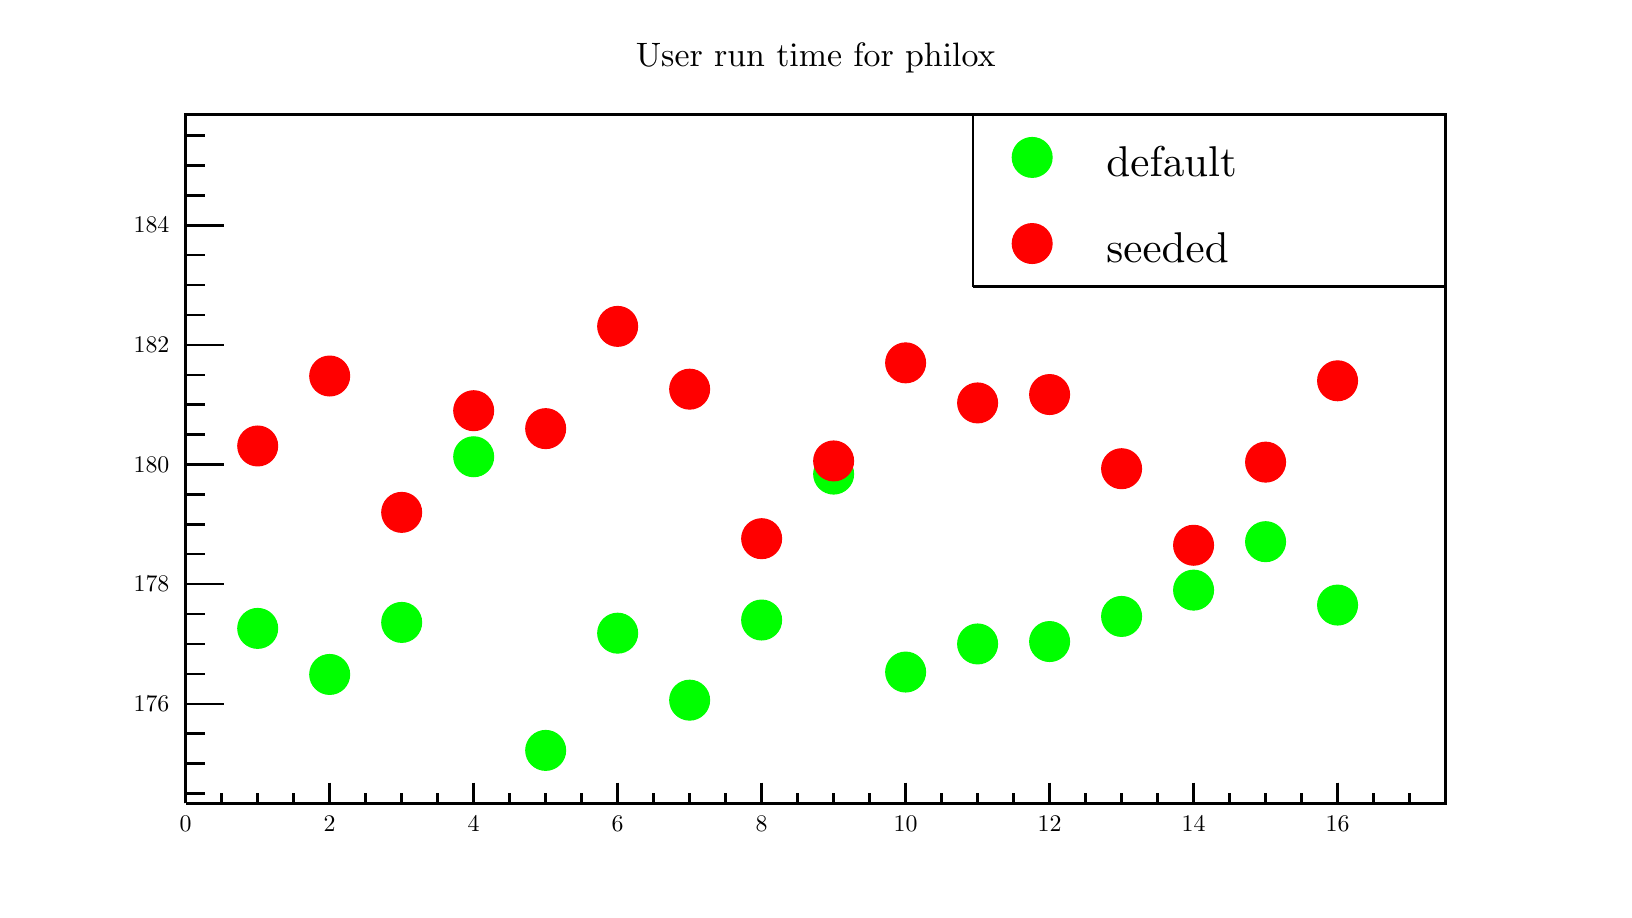
\begin{tikzpicture}
\pgfdeclareplotmark{cross} {
\pgfpathmoveto{\pgfpoint{-0.3\pgfplotmarksize}{\pgfplotmarksize}}
\pgfpathlineto{\pgfpoint{+0.3\pgfplotmarksize}{\pgfplotmarksize}}
\pgfpathlineto{\pgfpoint{+0.3\pgfplotmarksize}{0.3\pgfplotmarksize}}
\pgfpathlineto{\pgfpoint{+1\pgfplotmarksize}{0.3\pgfplotmarksize}}
\pgfpathlineto{\pgfpoint{+1\pgfplotmarksize}{-0.3\pgfplotmarksize}}
\pgfpathlineto{\pgfpoint{+0.3\pgfplotmarksize}{-0.3\pgfplotmarksize}}
\pgfpathlineto{\pgfpoint{+0.3\pgfplotmarksize}{-1.\pgfplotmarksize}}
\pgfpathlineto{\pgfpoint{-0.3\pgfplotmarksize}{-1.\pgfplotmarksize}}
\pgfpathlineto{\pgfpoint{-0.3\pgfplotmarksize}{-0.3\pgfplotmarksize}}
\pgfpathlineto{\pgfpoint{-1.\pgfplotmarksize}{-0.3\pgfplotmarksize}}
\pgfpathlineto{\pgfpoint{-1.\pgfplotmarksize}{0.3\pgfplotmarksize}}
\pgfpathlineto{\pgfpoint{-0.3\pgfplotmarksize}{0.3\pgfplotmarksize}}
\pgfpathclose
\pgfusepathqstroke
}
\pgfdeclareplotmark{cross*} {
\pgfpathmoveto{\pgfpoint{-0.3\pgfplotmarksize}{\pgfplotmarksize}}
\pgfpathlineto{\pgfpoint{+0.3\pgfplotmarksize}{\pgfplotmarksize}}
\pgfpathlineto{\pgfpoint{+0.3\pgfplotmarksize}{0.3\pgfplotmarksize}}
\pgfpathlineto{\pgfpoint{+1\pgfplotmarksize}{0.3\pgfplotmarksize}}
\pgfpathlineto{\pgfpoint{+1\pgfplotmarksize}{-0.3\pgfplotmarksize}}
\pgfpathlineto{\pgfpoint{+0.3\pgfplotmarksize}{-0.3\pgfplotmarksize}}
\pgfpathlineto{\pgfpoint{+0.3\pgfplotmarksize}{-1.\pgfplotmarksize}}
\pgfpathlineto{\pgfpoint{-0.3\pgfplotmarksize}{-1.\pgfplotmarksize}}
\pgfpathlineto{\pgfpoint{-0.3\pgfplotmarksize}{-0.3\pgfplotmarksize}}
\pgfpathlineto{\pgfpoint{-1.\pgfplotmarksize}{-0.3\pgfplotmarksize}}
\pgfpathlineto{\pgfpoint{-1.\pgfplotmarksize}{0.3\pgfplotmarksize}}
\pgfpathlineto{\pgfpoint{-0.3\pgfplotmarksize}{0.3\pgfplotmarksize}}
\pgfpathclose
\pgfusepathqfillstroke
}
\pgfdeclareplotmark{newstar} {
\pgfpathmoveto{\pgfqpoint{0pt}{\pgfplotmarksize}}
\pgfpathlineto{\pgfqpointpolar{44}{0.5\pgfplotmarksize}}
\pgfpathlineto{\pgfqpointpolar{18}{\pgfplotmarksize}}
\pgfpathlineto{\pgfqpointpolar{-20}{0.5\pgfplotmarksize}}
\pgfpathlineto{\pgfqpointpolar{-54}{\pgfplotmarksize}}
\pgfpathlineto{\pgfqpointpolar{-90}{0.5\pgfplotmarksize}}
\pgfpathlineto{\pgfqpointpolar{234}{\pgfplotmarksize}}
\pgfpathlineto{\pgfqpointpolar{198}{0.5\pgfplotmarksize}}
\pgfpathlineto{\pgfqpointpolar{162}{\pgfplotmarksize}}
\pgfpathlineto{\pgfqpointpolar{134}{0.5\pgfplotmarksize}}
\pgfpathclose
\pgfusepathqstroke
}
\pgfdeclareplotmark{newstar*} {
\pgfpathmoveto{\pgfqpoint{0pt}{\pgfplotmarksize}}
\pgfpathlineto{\pgfqpointpolar{44}{0.5\pgfplotmarksize}}
\pgfpathlineto{\pgfqpointpolar{18}{\pgfplotmarksize}}
\pgfpathlineto{\pgfqpointpolar{-20}{0.5\pgfplotmarksize}}
\pgfpathlineto{\pgfqpointpolar{-54}{\pgfplotmarksize}}
\pgfpathlineto{\pgfqpointpolar{-90}{0.5\pgfplotmarksize}}
\pgfpathlineto{\pgfqpointpolar{234}{\pgfplotmarksize}}
\pgfpathlineto{\pgfqpointpolar{198}{0.5\pgfplotmarksize}}
\pgfpathlineto{\pgfqpointpolar{162}{\pgfplotmarksize}}
\pgfpathlineto{\pgfqpointpolar{134}{0.5\pgfplotmarksize}}
\pgfpathclose
\pgfusepathqfillstroke
}
\definecolor{c}{rgb}{1,1,1};
\draw [color=c, fill=c] (0,0) rectangle (20,10.9387);
\draw [color=c, fill=c] (2,1.09387) rectangle (18,9.84481);
\definecolor{c}{rgb}{0,0,0};
\draw [c,line width=0.9] (2,1.09387) -- (2,9.84481) -- (18,9.84481) -- (18,1.09387) -- (2,1.09387);
\definecolor{c}{rgb}{1,1,1};
\draw [color=c, fill=c] (2,1.09387) rectangle (18,9.84481);
\definecolor{c}{rgb}{0,0,0};
\draw [c,line width=0.9] (2,1.09387) -- (2,9.84481) -- (18,9.84481) -- (18,1.09387) -- (2,1.09387);
\draw [c,line width=0.9] (2,1.09387) -- (18,1.09387);
\draw [c,line width=0.9] (2,1.3564) -- (2,1.09387);
\draw [c,line width=0.9] (2.45714,1.22513) -- (2.45714,1.09387);
\draw [c,line width=0.9] (2.91429,1.22513) -- (2.91429,1.09387);
\draw [c,line width=0.9] (3.37143,1.22513) -- (3.37143,1.09387);
\draw [c,line width=0.9] (3.82857,1.3564) -- (3.82857,1.09387);
\draw [c,line width=0.9] (4.28571,1.22513) -- (4.28571,1.09387);
\draw [c,line width=0.9] (4.74286,1.22513) -- (4.74286,1.09387);
\draw [c,line width=0.9] (5.2,1.22513) -- (5.2,1.09387);
\draw [c,line width=0.9] (5.65714,1.3564) -- (5.65714,1.09387);
\draw [c,line width=0.9] (6.11429,1.22513) -- (6.11429,1.09387);
\draw [c,line width=0.9] (6.57143,1.22513) -- (6.57143,1.09387);
\draw [c,line width=0.9] (7.02857,1.22513) -- (7.02857,1.09387);
\draw [c,line width=0.9] (7.48571,1.3564) -- (7.48571,1.09387);
\draw [c,line width=0.9] (7.94286,1.22513) -- (7.94286,1.09387);
\draw [c,line width=0.9] (8.4,1.22513) -- (8.4,1.09387);
\draw [c,line width=0.9] (8.85714,1.22513) -- (8.85714,1.09387);
\draw [c,line width=0.9] (9.31429,1.3564) -- (9.31429,1.09387);
\draw [c,line width=0.9] (9.77143,1.22513) -- (9.77143,1.09387);
\draw [c,line width=0.9] (10.2286,1.22513) -- (10.2286,1.09387);
\draw [c,line width=0.9] (10.6857,1.22513) -- (10.6857,1.09387);
\draw [c,line width=0.9] (11.1429,1.3564) -- (11.1429,1.09387);
\draw [c,line width=0.9] (11.6,1.22513) -- (11.6,1.09387);
\draw [c,line width=0.9] (12.0571,1.22513) -- (12.0571,1.09387);
\draw [c,line width=0.9] (12.5143,1.22513) -- (12.5143,1.09387);
\draw [c,line width=0.9] (12.9714,1.3564) -- (12.9714,1.09387);
\draw [c,line width=0.9] (13.4286,1.22513) -- (13.4286,1.09387);
\draw [c,line width=0.9] (13.8857,1.22513) -- (13.8857,1.09387);
\draw [c,line width=0.9] (14.3429,1.22513) -- (14.3429,1.09387);
\draw [c,line width=0.9] (14.8,1.3564) -- (14.8,1.09387);
\draw [c,line width=0.9] (15.2571,1.22513) -- (15.2571,1.09387);
\draw [c,line width=0.9] (15.7143,1.22513) -- (15.7143,1.09387);
\draw [c,line width=0.9] (16.1714,1.22513) -- (16.1714,1.09387);
\draw [c,line width=0.9] (16.6286,1.3564) -- (16.6286,1.09387);
\draw [c,line width=0.9] (16.6286,1.3564) -- (16.6286,1.09387);
\draw [c,line width=0.9] (17.0857,1.22513) -- (17.0857,1.09387);
\draw [c,line width=0.9] (17.5429,1.22513) -- (17.5429,1.09387);
\draw [c,line width=0.9] (18,1.22513) -- (18,1.09387);
\draw [anchor=base] (2,0.732891) node[scale=0.861703, color=c, rotate=0]{0};
\draw [anchor=base] (3.82857,0.732891) node[scale=0.861703, color=c, rotate=0]{2};
\draw [anchor=base] (5.65714,0.732891) node[scale=0.861703, color=c, rotate=0]{4};
\draw [anchor=base] (7.48571,0.732891) node[scale=0.861703, color=c, rotate=0]{6};
\draw [anchor=base] (9.31429,0.732891) node[scale=0.861703, color=c, rotate=0]{8};
\draw [anchor=base] (11.1429,0.732891) node[scale=0.861703, color=c, rotate=0]{10};
\draw [anchor=base] (12.9714,0.732891) node[scale=0.861703, color=c, rotate=0]{12};
\draw [anchor=base] (14.8,0.732891) node[scale=0.861703, color=c, rotate=0]{14};
\draw [anchor=base] (16.6286,0.732891) node[scale=0.861703, color=c, rotate=0]{16};
\draw [c,line width=0.9] (2,1.09387) -- (2,9.84481);
\draw [c,line width=0.9] (2.48,2.35946) -- (2,2.35946);
\draw [c,line width=0.9] (2.24,2.73924) -- (2,2.73924);
\draw [c,line width=0.9] (2.24,3.11901) -- (2,3.11901);
\draw [c,line width=0.9] (2.24,3.49879) -- (2,3.49879);
\draw [c,line width=0.9] (2.48,3.87856) -- (2,3.87856);
\draw [c,line width=0.9] (2.24,4.25833) -- (2,4.25833);
\draw [c,line width=0.9] (2.24,4.63811) -- (2,4.63811);
\draw [c,line width=0.9] (2.24,5.01788) -- (2,5.01788);
\draw [c,line width=0.9] (2.48,5.39765) -- (2,5.39765);
\draw [c,line width=0.9] (2.24,5.77743) -- (2,5.77743);
\draw [c,line width=0.9] (2.24,6.1572) -- (2,6.1572);
\draw [c,line width=0.9] (2.24,6.53698) -- (2,6.53698);
\draw [c,line width=0.9] (2.48,6.91675) -- (2,6.91675);
\draw [c,line width=0.9] (2.24,7.29652) -- (2,7.29652);
\draw [c,line width=0.9] (2.24,7.6763) -- (2,7.6763);
\draw [c,line width=0.9] (2.24,8.05607) -- (2,8.05607);
\draw [c,line width=0.9] (2.48,8.43584) -- (2,8.43584);
\draw [c,line width=0.9] (2.48,2.35946) -- (2,2.35946);
\draw [c,line width=0.9] (2.24,1.97969) -- (2,1.97969);
\draw [c,line width=0.9] (2.24,1.59992) -- (2,1.59992);
\draw [c,line width=0.9] (2.24,1.22014) -- (2,1.22014);
\draw [c,line width=0.9] (2.48,8.43584) -- (2,8.43584);
\draw [c,line width=0.9] (2.24,8.81562) -- (2,8.81562);
\draw [c,line width=0.9] (2.24,9.19539) -- (2,9.19539);
\draw [c,line width=0.9] (2.24,9.57517) -- (2,9.57517);
\draw [anchor= east] (1.9,2.35946) node[scale=0.861703, color=c, rotate=0]{176};
\draw [anchor= east] (1.9,3.87856) node[scale=0.861703, color=c, rotate=0]{178};
\draw [anchor= east] (1.9,5.39765) node[scale=0.861703, color=c, rotate=0]{180};
\draw [anchor= east] (1.9,6.91675) node[scale=0.861703, color=c, rotate=0]{182};
\draw [anchor= east] (1.9,8.43584) node[scale=0.861703, color=c, rotate=0]{184};
\definecolor{c}{rgb}{0,1,0};
\foreach \P in {(2.91429,3.31649), (3.82857,2.73164), (4.74286,3.39245), (5.65714,5.4964), (6.57143,1.76702), (7.48571,3.25573), (8.4,2.40504), (9.31429,3.42283), (10.2286,5.27613), (11.1429,2.76202), (12.0571,3.11901), (12.9714,3.14939),
 (13.8857,3.4684), (14.8,3.8026), (15.7143,4.41784), (16.6286,3.61272)}{\draw[mark options={color=c,fill=c},mark size=7.207207pt,mark=*] plot coordinates {\P};}
\definecolor{c}{rgb}{1,0,0};
\foreach \P in {(2.91429,5.63311), (3.82857,6.52178), (4.74286,4.79002), (5.65714,6.08125), (6.57143,5.85338), (7.48571,7.15221), (8.4,6.35468), (9.31429,4.45582), (10.2286,5.44323), (11.1429,6.68889), (12.0571,6.17999), (12.9714,6.28632),
 (13.8857,5.34449), (14.8,4.37226), (15.7143,5.42804), (16.6286,6.46102)}{\draw[mark options={color=c,fill=c},mark size=7.207207pt,mark=*] plot coordinates {\P};}
\definecolor{c}{rgb}{1,1,1};
\draw [color=c, fill=c] (12,7.65707) rectangle (18,9.84481);
\definecolor{c}{rgb}{0,0,0};
\draw [c,line width=0.9] (12,7.65707) -- (18,7.65707);
\draw [c,line width=0.9] (18,7.65707) -- (18,9.84481);
\draw [c,line width=0.9] (18,9.84481) -- (12,9.84481);
\draw [c,line width=0.9] (12,9.84481) -- (12,7.65707);
\draw [anchor=base west] (13.5,9.05175) node[scale=1.55662, color=c, rotate=0]{default};
\definecolor{c}{rgb}{1,1,1};
\draw [c] (12.225,8.91502) -- (13.275,8.91502) -- (13.275,9.68073) -- (12.225,9.68073);
\draw [c,line width=0.9] (12.225,9.29787) -- (13.275,9.29787);
\definecolor{c}{rgb}{0,1,0};
\foreach \P in {(12.75,9.29787)}{\draw[mark options={color=c,fill=c},mark size=7.207207pt,mark=*] plot coordinates {\P};}
\definecolor{c}{rgb}{0,0,0};
\draw [anchor=base west] (13.5,7.95788) node[scale=1.55662, color=c, rotate=0]{seeded};
\definecolor{c}{rgb}{1,1,1};
\draw [c] (12.225,7.82115) -- (13.275,7.82115) -- (13.275,8.58686) -- (12.225,8.58686);
\draw [c,line width=0.9] (12.225,8.204) -- (13.275,8.204);
\definecolor{c}{rgb}{1,0,0};
\foreach \P in {(12.75,8.204)}{\draw[mark options={color=c,fill=c},mark size=7.207207pt,mark=*] plot coordinates {\P};}
\definecolor{c}{rgb}{0,0,0};
\draw (10,10.5611) node[scale=1.22306, color=c, rotate=0]{User run time for philox};
\end{tikzpicture}
}
    \scalebox{.8}{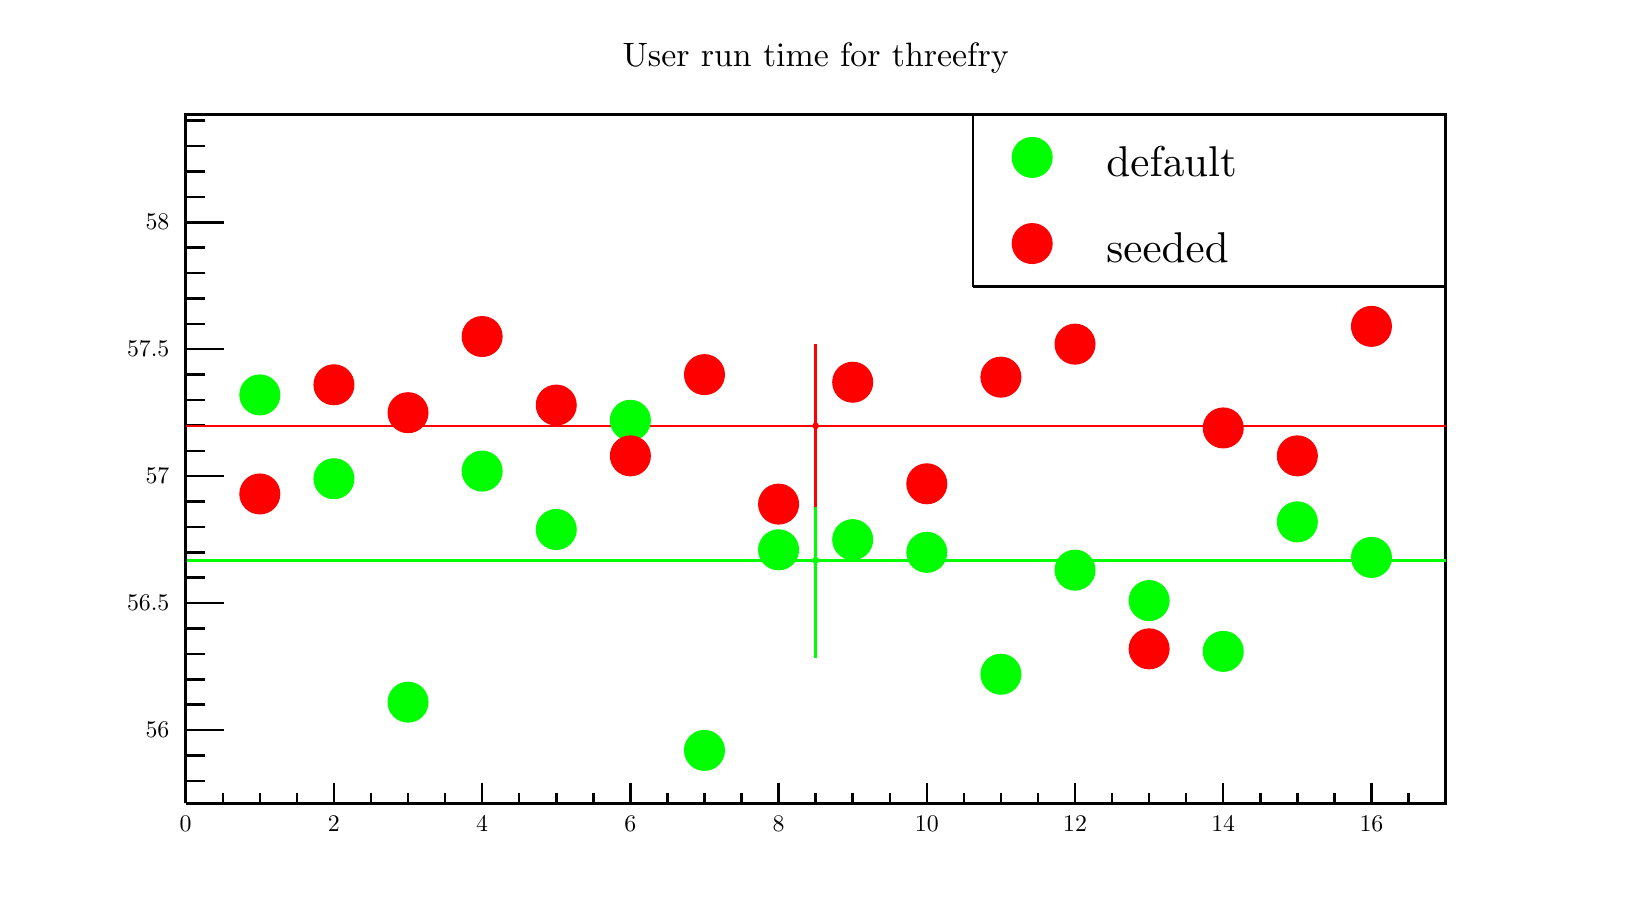
\begin{tikzpicture}
\pgfdeclareplotmark{cross} {
\pgfpathmoveto{\pgfpoint{-0.3\pgfplotmarksize}{\pgfplotmarksize}}
\pgfpathlineto{\pgfpoint{+0.3\pgfplotmarksize}{\pgfplotmarksize}}
\pgfpathlineto{\pgfpoint{+0.3\pgfplotmarksize}{0.3\pgfplotmarksize}}
\pgfpathlineto{\pgfpoint{+1\pgfplotmarksize}{0.3\pgfplotmarksize}}
\pgfpathlineto{\pgfpoint{+1\pgfplotmarksize}{-0.3\pgfplotmarksize}}
\pgfpathlineto{\pgfpoint{+0.3\pgfplotmarksize}{-0.3\pgfplotmarksize}}
\pgfpathlineto{\pgfpoint{+0.3\pgfplotmarksize}{-1.\pgfplotmarksize}}
\pgfpathlineto{\pgfpoint{-0.3\pgfplotmarksize}{-1.\pgfplotmarksize}}
\pgfpathlineto{\pgfpoint{-0.3\pgfplotmarksize}{-0.3\pgfplotmarksize}}
\pgfpathlineto{\pgfpoint{-1.\pgfplotmarksize}{-0.3\pgfplotmarksize}}
\pgfpathlineto{\pgfpoint{-1.\pgfplotmarksize}{0.3\pgfplotmarksize}}
\pgfpathlineto{\pgfpoint{-0.3\pgfplotmarksize}{0.3\pgfplotmarksize}}
\pgfpathclose
\pgfusepathqstroke
}
\pgfdeclareplotmark{cross*} {
\pgfpathmoveto{\pgfpoint{-0.3\pgfplotmarksize}{\pgfplotmarksize}}
\pgfpathlineto{\pgfpoint{+0.3\pgfplotmarksize}{\pgfplotmarksize}}
\pgfpathlineto{\pgfpoint{+0.3\pgfplotmarksize}{0.3\pgfplotmarksize}}
\pgfpathlineto{\pgfpoint{+1\pgfplotmarksize}{0.3\pgfplotmarksize}}
\pgfpathlineto{\pgfpoint{+1\pgfplotmarksize}{-0.3\pgfplotmarksize}}
\pgfpathlineto{\pgfpoint{+0.3\pgfplotmarksize}{-0.3\pgfplotmarksize}}
\pgfpathlineto{\pgfpoint{+0.3\pgfplotmarksize}{-1.\pgfplotmarksize}}
\pgfpathlineto{\pgfpoint{-0.3\pgfplotmarksize}{-1.\pgfplotmarksize}}
\pgfpathlineto{\pgfpoint{-0.3\pgfplotmarksize}{-0.3\pgfplotmarksize}}
\pgfpathlineto{\pgfpoint{-1.\pgfplotmarksize}{-0.3\pgfplotmarksize}}
\pgfpathlineto{\pgfpoint{-1.\pgfplotmarksize}{0.3\pgfplotmarksize}}
\pgfpathlineto{\pgfpoint{-0.3\pgfplotmarksize}{0.3\pgfplotmarksize}}
\pgfpathclose
\pgfusepathqfillstroke
}
\pgfdeclareplotmark{newstar} {
\pgfpathmoveto{\pgfqpoint{0pt}{\pgfplotmarksize}}
\pgfpathlineto{\pgfqpointpolar{44}{0.5\pgfplotmarksize}}
\pgfpathlineto{\pgfqpointpolar{18}{\pgfplotmarksize}}
\pgfpathlineto{\pgfqpointpolar{-20}{0.5\pgfplotmarksize}}
\pgfpathlineto{\pgfqpointpolar{-54}{\pgfplotmarksize}}
\pgfpathlineto{\pgfqpointpolar{-90}{0.5\pgfplotmarksize}}
\pgfpathlineto{\pgfqpointpolar{234}{\pgfplotmarksize}}
\pgfpathlineto{\pgfqpointpolar{198}{0.5\pgfplotmarksize}}
\pgfpathlineto{\pgfqpointpolar{162}{\pgfplotmarksize}}
\pgfpathlineto{\pgfqpointpolar{134}{0.5\pgfplotmarksize}}
\pgfpathclose
\pgfusepathqstroke
}
\pgfdeclareplotmark{newstar*} {
\pgfpathmoveto{\pgfqpoint{0pt}{\pgfplotmarksize}}
\pgfpathlineto{\pgfqpointpolar{44}{0.5\pgfplotmarksize}}
\pgfpathlineto{\pgfqpointpolar{18}{\pgfplotmarksize}}
\pgfpathlineto{\pgfqpointpolar{-20}{0.5\pgfplotmarksize}}
\pgfpathlineto{\pgfqpointpolar{-54}{\pgfplotmarksize}}
\pgfpathlineto{\pgfqpointpolar{-90}{0.5\pgfplotmarksize}}
\pgfpathlineto{\pgfqpointpolar{234}{\pgfplotmarksize}}
\pgfpathlineto{\pgfqpointpolar{198}{0.5\pgfplotmarksize}}
\pgfpathlineto{\pgfqpointpolar{162}{\pgfplotmarksize}}
\pgfpathlineto{\pgfqpointpolar{134}{0.5\pgfplotmarksize}}
\pgfpathclose
\pgfusepathqfillstroke
}
\definecolor{c}{rgb}{1,1,1};
\draw [color=c, fill=c] (0,0) rectangle (20,10.9387);
\draw [color=c, fill=c] (2,1.09387) rectangle (18,9.84481);
\definecolor{c}{rgb}{0,0,0};
\draw [c,line width=0.9] (2,1.09387) -- (2,9.84481) -- (18,9.84481) -- (18,1.09387) -- (2,1.09387);
\definecolor{c}{rgb}{1,1,1};
\draw [color=c, fill=c] (2,1.09387) rectangle (18,9.84481);
\definecolor{c}{rgb}{0,0,0};
\draw [c,line width=0.9] (2,1.09387) -- (2,9.84481) -- (18,9.84481) -- (18,1.09387) -- (2,1.09387);
\definecolor{c}{rgb}{0,1,0};
\draw [c,line width=0.9] (10,2.93782) -- (10,4.18149);
\draw [c,line width=0.9] (10,4.18149) -- (10,5.42516);
\draw [c,line width=0.9] (2,4.18149) -- (10,4.18149);
\draw [c,line width=0.9] (10,4.18149) -- (18,4.18149);
\foreach \P in {(10,4.18149)}{\draw[mark options={color=c,fill=c},mark size=2.402402pt,mark=*,mark size=1pt] plot coordinates {\P};}
\definecolor{c}{rgb}{0,0,0};
\draw [c,line width=0.9] (2,1.09387) -- (18,1.09387);
\draw [c,line width=0.9] (2,1.3564) -- (2,1.09387);
\draw [c,line width=0.9] (2.47059,1.22513) -- (2.47059,1.09387);
\draw [c,line width=0.9] (2.94118,1.22513) -- (2.94118,1.09387);
\draw [c,line width=0.9] (3.41176,1.22513) -- (3.41176,1.09387);
\draw [c,line width=0.9] (3.88235,1.3564) -- (3.88235,1.09387);
\draw [c,line width=0.9] (4.35294,1.22513) -- (4.35294,1.09387);
\draw [c,line width=0.9] (4.82353,1.22513) -- (4.82353,1.09387);
\draw [c,line width=0.9] (5.29412,1.22513) -- (5.29412,1.09387);
\draw [c,line width=0.9] (5.76471,1.3564) -- (5.76471,1.09387);
\draw [c,line width=0.9] (6.23529,1.22513) -- (6.23529,1.09387);
\draw [c,line width=0.9] (6.70588,1.22513) -- (6.70588,1.09387);
\draw [c,line width=0.9] (7.17647,1.22513) -- (7.17647,1.09387);
\draw [c,line width=0.9] (7.64706,1.3564) -- (7.64706,1.09387);
\draw [c,line width=0.9] (8.11765,1.22513) -- (8.11765,1.09387);
\draw [c,line width=0.9] (8.58823,1.22513) -- (8.58823,1.09387);
\draw [c,line width=0.9] (9.05882,1.22513) -- (9.05882,1.09387);
\draw [c,line width=0.9] (9.52941,1.3564) -- (9.52941,1.09387);
\draw [c,line width=0.9] (10,1.22513) -- (10,1.09387);
\draw [c,line width=0.9] (10.4706,1.22513) -- (10.4706,1.09387);
\draw [c,line width=0.9] (10.9412,1.22513) -- (10.9412,1.09387);
\draw [c,line width=0.9] (11.4118,1.3564) -- (11.4118,1.09387);
\draw [c,line width=0.9] (11.8824,1.22513) -- (11.8824,1.09387);
\draw [c,line width=0.9] (12.3529,1.22513) -- (12.3529,1.09387);
\draw [c,line width=0.9] (12.8235,1.22513) -- (12.8235,1.09387);
\draw [c,line width=0.9] (13.2941,1.3564) -- (13.2941,1.09387);
\draw [c,line width=0.9] (13.7647,1.22513) -- (13.7647,1.09387);
\draw [c,line width=0.9] (14.2353,1.22513) -- (14.2353,1.09387);
\draw [c,line width=0.9] (14.7059,1.22513) -- (14.7059,1.09387);
\draw [c,line width=0.9] (15.1765,1.3564) -- (15.1765,1.09387);
\draw [c,line width=0.9] (15.6471,1.22513) -- (15.6471,1.09387);
\draw [c,line width=0.9] (16.1176,1.22513) -- (16.1176,1.09387);
\draw [c,line width=0.9] (16.5882,1.22513) -- (16.5882,1.09387);
\draw [c,line width=0.9] (17.0588,1.3564) -- (17.0588,1.09387);
\draw [c,line width=0.9] (17.0588,1.3564) -- (17.0588,1.09387);
\draw [c,line width=0.9] (17.5294,1.22513) -- (17.5294,1.09387);
\draw [c,line width=0.9] (18,1.22513) -- (18,1.09387);
\draw [anchor=base] (2,0.732891) node[scale=0.861703, color=c, rotate=0]{0};
\draw [anchor=base] (3.88235,0.732891) node[scale=0.861703, color=c, rotate=0]{2};
\draw [anchor=base] (5.76471,0.732891) node[scale=0.861703, color=c, rotate=0]{4};
\draw [anchor=base] (7.64706,0.732891) node[scale=0.861703, color=c, rotate=0]{6};
\draw [anchor=base] (9.52941,0.732891) node[scale=0.861703, color=c, rotate=0]{8};
\draw [anchor=base] (11.4118,0.732891) node[scale=0.861703, color=c, rotate=0]{10};
\draw [anchor=base] (13.2941,0.732891) node[scale=0.861703, color=c, rotate=0]{12};
\draw [anchor=base] (15.1765,0.732891) node[scale=0.861703, color=c, rotate=0]{14};
\draw [anchor=base] (17.0588,0.732891) node[scale=0.861703, color=c, rotate=0]{16};
\draw [c,line width=0.9] (2,1.09387) -- (2,9.84481);
\draw [c,line width=0.9] (2.48,2.02499) -- (2,2.02499);
\draw [c,line width=0.9] (2.24,2.34746) -- (2,2.34746);
\draw [c,line width=0.9] (2.24,2.66992) -- (2,2.66992);
\draw [c,line width=0.9] (2.24,2.99239) -- (2,2.99239);
\draw [c,line width=0.9] (2.24,3.31486) -- (2,3.31486);
\draw [c,line width=0.9] (2.48,3.63732) -- (2,3.63732);
\draw [c,line width=0.9] (2.24,3.95979) -- (2,3.95979);
\draw [c,line width=0.9] (2.24,4.28226) -- (2,4.28226);
\draw [c,line width=0.9] (2.24,4.60472) -- (2,4.60472);
\draw [c,line width=0.9] (2.24,4.92719) -- (2,4.92719);
\draw [c,line width=0.9] (2.48,5.24966) -- (2,5.24966);
\draw [c,line width=0.9] (2.24,5.57212) -- (2,5.57212);
\draw [c,line width=0.9] (2.24,5.89459) -- (2,5.89459);
\draw [c,line width=0.9] (2.24,6.21706) -- (2,6.21706);
\draw [c,line width=0.9] (2.24,6.53952) -- (2,6.53952);
\draw [c,line width=0.9] (2.48,6.86199) -- (2,6.86199);
\draw [c,line width=0.9] (2.24,7.18446) -- (2,7.18446);
\draw [c,line width=0.9] (2.24,7.50692) -- (2,7.50692);
\draw [c,line width=0.9] (2.24,7.82939) -- (2,7.82939);
\draw [c,line width=0.9] (2.24,8.15186) -- (2,8.15186);
\draw [c,line width=0.9] (2.48,8.47432) -- (2,8.47432);
\draw [c,line width=0.9] (2.48,2.02499) -- (2,2.02499);
\draw [c,line width=0.9] (2.24,1.70252) -- (2,1.70252);
\draw [c,line width=0.9] (2.24,1.38006) -- (2,1.38006);
\draw [c,line width=0.9] (2.48,8.47432) -- (2,8.47432);
\draw [c,line width=0.9] (2.24,8.79679) -- (2,8.79679);
\draw [c,line width=0.9] (2.24,9.11926) -- (2,9.11926);
\draw [c,line width=0.9] (2.24,9.44172) -- (2,9.44172);
\draw [c,line width=0.9] (2.24,9.76419) -- (2,9.76419);
\draw [anchor= east] (1.9,2.02499) node[scale=0.861703, color=c, rotate=0]{56};
\draw [anchor= east] (1.9,3.63732) node[scale=0.861703, color=c, rotate=0]{56.5};
\draw [anchor= east] (1.9,5.24966) node[scale=0.861703, color=c, rotate=0]{57};
\draw [anchor= east] (1.9,6.86199) node[scale=0.861703, color=c, rotate=0]{57.5};
\draw [anchor= east] (1.9,8.47432) node[scale=0.861703, color=c, rotate=0]{58};
\definecolor{c}{rgb}{1,0,0};
\draw [c,line width=0.9] (10,4.85475) -- (10,5.88854);
\draw [c,line width=0.9] (10,5.88854) -- (10,6.92233);
\draw [c,line width=0.9] (2,5.88854) -- (10,5.88854);
\draw [c,line width=0.9] (10,5.88854) -- (18,5.88854);
\foreach \P in {(10,5.88854)}{\draw[mark options={color=c,fill=c},mark size=2.402402pt,mark=*,mark size=1pt] plot coordinates {\P};}
\definecolor{c}{rgb}{0,1,0};
\foreach \P in {(2.94118,6.28155), (3.88235,5.21741), (4.82353,2.3797), (5.76471,5.31415), (6.70588,4.57248), (7.64706,5.95908), (8.58823,1.76702), (9.52941,4.3145), (10.4706,4.44349), (11.4118,4.28226), (12.3529,2.73442), (13.2941,4.05653),
 (14.2353,3.66957), (15.1765,3.02464), (16.1176,4.66922), (17.0588,4.21776)}{\draw[mark options={color=c,fill=c},mark size=7.207207pt,mark=*] plot coordinates {\P};}
\definecolor{c}{rgb}{1,0,0};
\foreach \P in {(2.94118,5.02393), (3.88235,6.41054), (4.82353,6.05582), (5.76471,7.02322), (6.70588,6.15256), (7.64706,5.50763), (8.58823,6.53952), (9.52941,4.89494), (10.4706,6.44278), (11.4118,5.15292), (12.3529,6.50728), (13.2941,6.92648),
 (14.2353,3.05688), (15.1765,5.86234), (16.1176,5.50763), (17.0588,7.15221)}{\draw[mark options={color=c,fill=c},mark size=7.207207pt,mark=*] plot coordinates {\P};}
\definecolor{c}{rgb}{1,1,1};
\draw [color=c, fill=c] (12,7.65707) rectangle (18,9.84481);
\definecolor{c}{rgb}{0,0,0};
\draw [c,line width=0.9] (12,7.65707) -- (18,7.65707);
\draw [c,line width=0.9] (18,7.65707) -- (18,9.84481);
\draw [c,line width=0.9] (18,9.84481) -- (12,9.84481);
\draw [c,line width=0.9] (12,9.84481) -- (12,7.65707);
\draw [anchor=base west] (13.5,9.05175) node[scale=1.55662, color=c, rotate=0]{default};
\definecolor{c}{rgb}{1,1,1};
\draw [c] (12.225,8.91502) -- (13.275,8.91502) -- (13.275,9.68073) -- (12.225,9.68073);
\draw [c,line width=0.9] (12.225,9.29787) -- (13.275,9.29787);
\definecolor{c}{rgb}{0,1,0};
\foreach \P in {(12.75,9.29787)}{\draw[mark options={color=c,fill=c},mark size=7.207207pt,mark=*] plot coordinates {\P};}
\definecolor{c}{rgb}{0,0,0};
\draw [anchor=base west] (13.5,7.95788) node[scale=1.55662, color=c, rotate=0]{seeded};
\definecolor{c}{rgb}{1,1,1};
\draw [c] (12.225,7.82115) -- (13.275,7.82115) -- (13.275,8.58686) -- (12.225,8.58686);
\draw [c,line width=0.9] (12.225,8.20401) -- (13.275,8.20401);
\definecolor{c}{rgb}{1,0,0};
\foreach \P in {(12.75,8.20401)}{\draw[mark options={color=c,fill=c},mark size=7.207207pt,mark=*] plot coordinates {\P};}
\definecolor{c}{rgb}{0,0,0};
\draw (10,10.5611) node[scale=1.22306, color=c, rotate=0]{User run time for threefry};
\end{tikzpicture}
}
    \scalebox{.8}{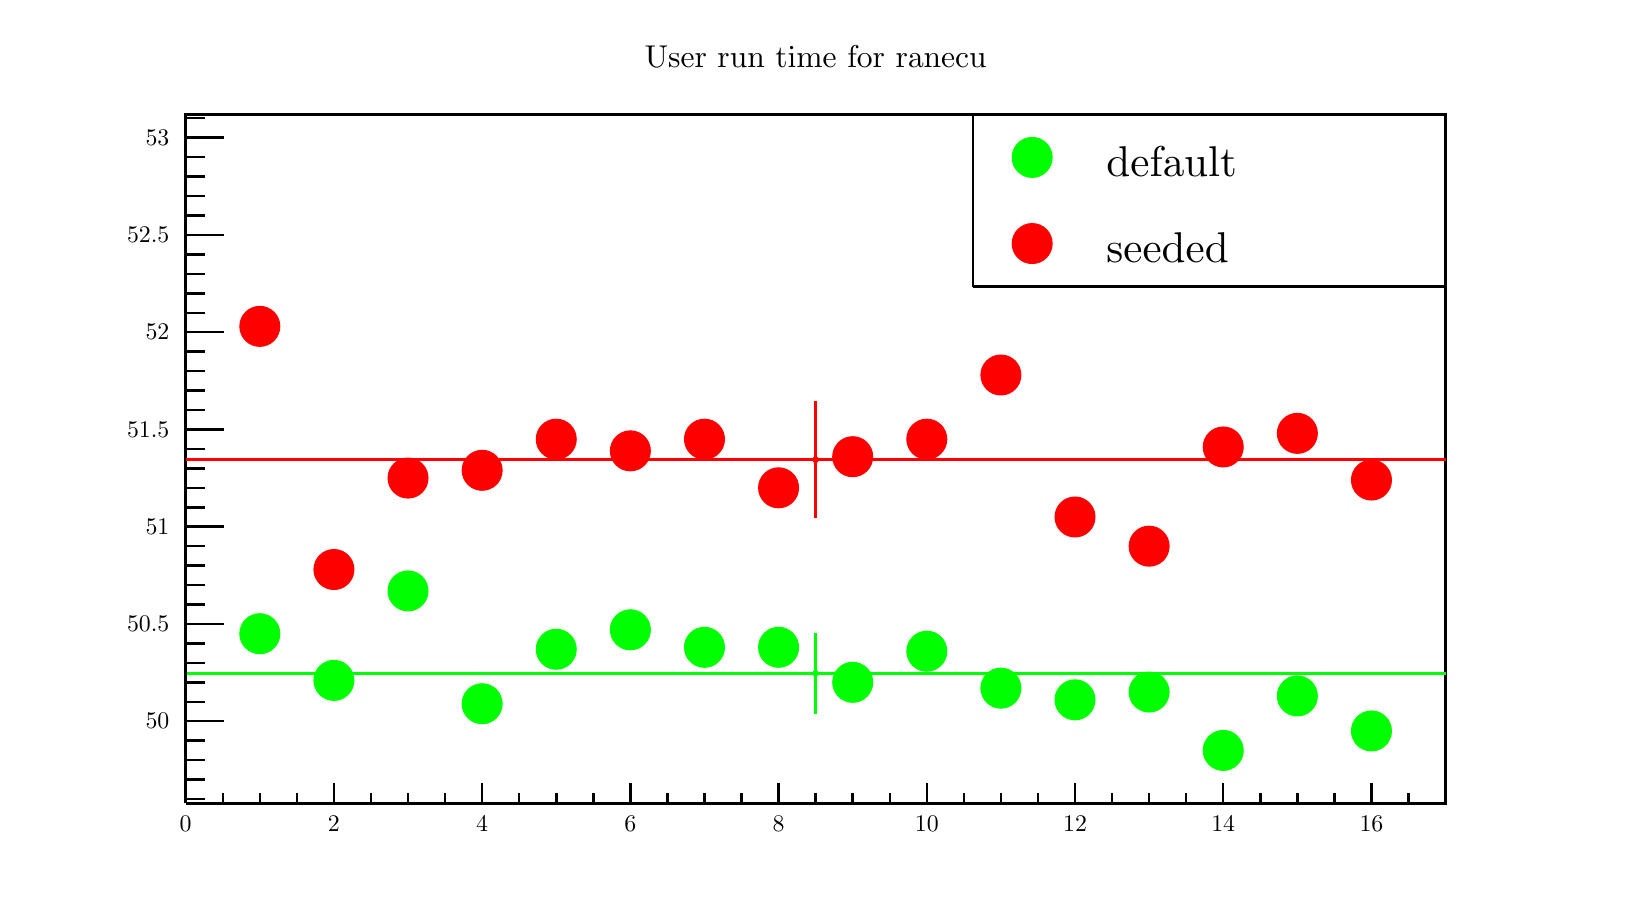
\begin{tikzpicture}
\pgfdeclareplotmark{cross} {
\pgfpathmoveto{\pgfpoint{-0.3\pgfplotmarksize}{\pgfplotmarksize}}
\pgfpathlineto{\pgfpoint{+0.3\pgfplotmarksize}{\pgfplotmarksize}}
\pgfpathlineto{\pgfpoint{+0.3\pgfplotmarksize}{0.3\pgfplotmarksize}}
\pgfpathlineto{\pgfpoint{+1\pgfplotmarksize}{0.3\pgfplotmarksize}}
\pgfpathlineto{\pgfpoint{+1\pgfplotmarksize}{-0.3\pgfplotmarksize}}
\pgfpathlineto{\pgfpoint{+0.3\pgfplotmarksize}{-0.3\pgfplotmarksize}}
\pgfpathlineto{\pgfpoint{+0.3\pgfplotmarksize}{-1.\pgfplotmarksize}}
\pgfpathlineto{\pgfpoint{-0.3\pgfplotmarksize}{-1.\pgfplotmarksize}}
\pgfpathlineto{\pgfpoint{-0.3\pgfplotmarksize}{-0.3\pgfplotmarksize}}
\pgfpathlineto{\pgfpoint{-1.\pgfplotmarksize}{-0.3\pgfplotmarksize}}
\pgfpathlineto{\pgfpoint{-1.\pgfplotmarksize}{0.3\pgfplotmarksize}}
\pgfpathlineto{\pgfpoint{-0.3\pgfplotmarksize}{0.3\pgfplotmarksize}}
\pgfpathclose
\pgfusepathqstroke
}
\pgfdeclareplotmark{cross*} {
\pgfpathmoveto{\pgfpoint{-0.3\pgfplotmarksize}{\pgfplotmarksize}}
\pgfpathlineto{\pgfpoint{+0.3\pgfplotmarksize}{\pgfplotmarksize}}
\pgfpathlineto{\pgfpoint{+0.3\pgfplotmarksize}{0.3\pgfplotmarksize}}
\pgfpathlineto{\pgfpoint{+1\pgfplotmarksize}{0.3\pgfplotmarksize}}
\pgfpathlineto{\pgfpoint{+1\pgfplotmarksize}{-0.3\pgfplotmarksize}}
\pgfpathlineto{\pgfpoint{+0.3\pgfplotmarksize}{-0.3\pgfplotmarksize}}
\pgfpathlineto{\pgfpoint{+0.3\pgfplotmarksize}{-1.\pgfplotmarksize}}
\pgfpathlineto{\pgfpoint{-0.3\pgfplotmarksize}{-1.\pgfplotmarksize}}
\pgfpathlineto{\pgfpoint{-0.3\pgfplotmarksize}{-0.3\pgfplotmarksize}}
\pgfpathlineto{\pgfpoint{-1.\pgfplotmarksize}{-0.3\pgfplotmarksize}}
\pgfpathlineto{\pgfpoint{-1.\pgfplotmarksize}{0.3\pgfplotmarksize}}
\pgfpathlineto{\pgfpoint{-0.3\pgfplotmarksize}{0.3\pgfplotmarksize}}
\pgfpathclose
\pgfusepathqfillstroke
}
\pgfdeclareplotmark{newstar} {
\pgfpathmoveto{\pgfqpoint{0pt}{\pgfplotmarksize}}
\pgfpathlineto{\pgfqpointpolar{44}{0.5\pgfplotmarksize}}
\pgfpathlineto{\pgfqpointpolar{18}{\pgfplotmarksize}}
\pgfpathlineto{\pgfqpointpolar{-20}{0.5\pgfplotmarksize}}
\pgfpathlineto{\pgfqpointpolar{-54}{\pgfplotmarksize}}
\pgfpathlineto{\pgfqpointpolar{-90}{0.5\pgfplotmarksize}}
\pgfpathlineto{\pgfqpointpolar{234}{\pgfplotmarksize}}
\pgfpathlineto{\pgfqpointpolar{198}{0.5\pgfplotmarksize}}
\pgfpathlineto{\pgfqpointpolar{162}{\pgfplotmarksize}}
\pgfpathlineto{\pgfqpointpolar{134}{0.5\pgfplotmarksize}}
\pgfpathclose
\pgfusepathqstroke
}
\pgfdeclareplotmark{newstar*} {
\pgfpathmoveto{\pgfqpoint{0pt}{\pgfplotmarksize}}
\pgfpathlineto{\pgfqpointpolar{44}{0.5\pgfplotmarksize}}
\pgfpathlineto{\pgfqpointpolar{18}{\pgfplotmarksize}}
\pgfpathlineto{\pgfqpointpolar{-20}{0.5\pgfplotmarksize}}
\pgfpathlineto{\pgfqpointpolar{-54}{\pgfplotmarksize}}
\pgfpathlineto{\pgfqpointpolar{-90}{0.5\pgfplotmarksize}}
\pgfpathlineto{\pgfqpointpolar{234}{\pgfplotmarksize}}
\pgfpathlineto{\pgfqpointpolar{198}{0.5\pgfplotmarksize}}
\pgfpathlineto{\pgfqpointpolar{162}{\pgfplotmarksize}}
\pgfpathlineto{\pgfqpointpolar{134}{0.5\pgfplotmarksize}}
\pgfpathclose
\pgfusepathqfillstroke
}
\definecolor{c}{rgb}{1,1,1};
\draw [color=c, fill=c] (0,0) rectangle (20,10.9387);
\draw [color=c, fill=c] (2,1.09387) rectangle (18,9.84481);
\definecolor{c}{rgb}{0,0,0};
\draw [c,line width=0.9] (2,1.09387) -- (2,9.84481) -- (18,9.84481) -- (18,1.09387) -- (2,1.09387);
\definecolor{c}{rgb}{1,1,1};
\draw [color=c, fill=c] (2,1.09387) rectangle (18,9.84481);
\definecolor{c}{rgb}{0,0,0};
\draw [c,line width=0.9] (2,1.09387) -- (2,9.84481) -- (18,9.84481) -- (18,1.09387) -- (2,1.09387);
\definecolor{c}{rgb}{0,1,0};
\draw [c,line width=0.9] (10,2.22967) -- (10,2.74586);
\draw [c,line width=0.9] (10,2.74586) -- (10,3.26205);
\draw [c,line width=0.9] (2,2.74586) -- (10,2.74586);
\draw [c,line width=0.9] (10,2.74586) -- (18,2.74586);
\foreach \P in {(10,2.74586)}{\draw[mark options={color=c,fill=c},mark size=2.402402pt,mark=*,mark size=1pt] plot coordinates {\P};}
\definecolor{c}{rgb}{0,0,0};
\draw [c,line width=0.9] (2,1.09387) -- (18,1.09387);
\draw [c,line width=0.9] (2,1.3564) -- (2,1.09387);
\draw [c,line width=0.9] (2.47059,1.22513) -- (2.47059,1.09387);
\draw [c,line width=0.9] (2.94118,1.22513) -- (2.94118,1.09387);
\draw [c,line width=0.9] (3.41176,1.22513) -- (3.41176,1.09387);
\draw [c,line width=0.9] (3.88235,1.3564) -- (3.88235,1.09387);
\draw [c,line width=0.9] (4.35294,1.22513) -- (4.35294,1.09387);
\draw [c,line width=0.9] (4.82353,1.22513) -- (4.82353,1.09387);
\draw [c,line width=0.9] (5.29412,1.22513) -- (5.29412,1.09387);
\draw [c,line width=0.9] (5.76471,1.3564) -- (5.76471,1.09387);
\draw [c,line width=0.9] (6.23529,1.22513) -- (6.23529,1.09387);
\draw [c,line width=0.9] (6.70588,1.22513) -- (6.70588,1.09387);
\draw [c,line width=0.9] (7.17647,1.22513) -- (7.17647,1.09387);
\draw [c,line width=0.9] (7.64706,1.3564) -- (7.64706,1.09387);
\draw [c,line width=0.9] (8.11765,1.22513) -- (8.11765,1.09387);
\draw [c,line width=0.9] (8.58823,1.22513) -- (8.58823,1.09387);
\draw [c,line width=0.9] (9.05882,1.22513) -- (9.05882,1.09387);
\draw [c,line width=0.9] (9.52941,1.3564) -- (9.52941,1.09387);
\draw [c,line width=0.9] (10,1.22513) -- (10,1.09387);
\draw [c,line width=0.9] (10.4706,1.22513) -- (10.4706,1.09387);
\draw [c,line width=0.9] (10.9412,1.22513) -- (10.9412,1.09387);
\draw [c,line width=0.9] (11.4118,1.3564) -- (11.4118,1.09387);
\draw [c,line width=0.9] (11.8824,1.22513) -- (11.8824,1.09387);
\draw [c,line width=0.9] (12.3529,1.22513) -- (12.3529,1.09387);
\draw [c,line width=0.9] (12.8235,1.22513) -- (12.8235,1.09387);
\draw [c,line width=0.9] (13.2941,1.3564) -- (13.2941,1.09387);
\draw [c,line width=0.9] (13.7647,1.22513) -- (13.7647,1.09387);
\draw [c,line width=0.9] (14.2353,1.22513) -- (14.2353,1.09387);
\draw [c,line width=0.9] (14.7059,1.22513) -- (14.7059,1.09387);
\draw [c,line width=0.9] (15.1765,1.3564) -- (15.1765,1.09387);
\draw [c,line width=0.9] (15.6471,1.22513) -- (15.6471,1.09387);
\draw [c,line width=0.9] (16.1176,1.22513) -- (16.1176,1.09387);
\draw [c,line width=0.9] (16.5882,1.22513) -- (16.5882,1.09387);
\draw [c,line width=0.9] (17.0588,1.3564) -- (17.0588,1.09387);
\draw [c,line width=0.9] (17.0588,1.3564) -- (17.0588,1.09387);
\draw [c,line width=0.9] (17.5294,1.22513) -- (17.5294,1.09387);
\draw [c,line width=0.9] (18,1.22513) -- (18,1.09387);
\draw [anchor=base] (2,0.732891) node[scale=0.861703, color=c, rotate=0]{0};
\draw [anchor=base] (3.88235,0.732891) node[scale=0.861703, color=c, rotate=0]{2};
\draw [anchor=base] (5.76471,0.732891) node[scale=0.861703, color=c, rotate=0]{4};
\draw [anchor=base] (7.64706,0.732891) node[scale=0.861703, color=c, rotate=0]{6};
\draw [anchor=base] (9.52941,0.732891) node[scale=0.861703, color=c, rotate=0]{8};
\draw [anchor=base] (11.4118,0.732891) node[scale=0.861703, color=c, rotate=0]{10};
\draw [anchor=base] (13.2941,0.732891) node[scale=0.861703, color=c, rotate=0]{12};
\draw [anchor=base] (15.1765,0.732891) node[scale=0.861703, color=c, rotate=0]{14};
\draw [anchor=base] (17.0588,0.732891) node[scale=0.861703, color=c, rotate=0]{16};
\draw [c,line width=0.9] (2,1.09387) -- (2,9.84481);
\draw [c,line width=0.9] (2.48,2.13756) -- (2,2.13756);
\draw [c,line width=0.9] (2.24,2.38458) -- (2,2.38458);
\draw [c,line width=0.9] (2.24,2.63161) -- (2,2.63161);
\draw [c,line width=0.9] (2.24,2.87864) -- (2,2.87864);
\draw [c,line width=0.9] (2.24,3.12567) -- (2,3.12567);
\draw [c,line width=0.9] (2.48,3.37269) -- (2,3.37269);
\draw [c,line width=0.9] (2.24,3.61972) -- (2,3.61972);
\draw [c,line width=0.9] (2.24,3.86675) -- (2,3.86675);
\draw [c,line width=0.9] (2.24,4.11377) -- (2,4.11377);
\draw [c,line width=0.9] (2.24,4.3608) -- (2,4.3608);
\draw [c,line width=0.9] (2.48,4.60783) -- (2,4.60783);
\draw [c,line width=0.9] (2.24,4.85486) -- (2,4.85486);
\draw [c,line width=0.9] (2.24,5.10188) -- (2,5.10188);
\draw [c,line width=0.9] (2.24,5.34891) -- (2,5.34891);
\draw [c,line width=0.9] (2.24,5.59594) -- (2,5.59594);
\draw [c,line width=0.9] (2.48,5.84297) -- (2,5.84297);
\draw [c,line width=0.9] (2.24,6.08999) -- (2,6.08999);
\draw [c,line width=0.9] (2.24,6.33702) -- (2,6.33702);
\draw [c,line width=0.9] (2.24,6.58405) -- (2,6.58405);
\draw [c,line width=0.9] (2.24,6.83107) -- (2,6.83107);
\draw [c,line width=0.9] (2.48,7.0781) -- (2,7.0781);
\draw [c,line width=0.9] (2.24,7.32513) -- (2,7.32513);
\draw [c,line width=0.9] (2.24,7.57216) -- (2,7.57216);
\draw [c,line width=0.9] (2.24,7.81918) -- (2,7.81918);
\draw [c,line width=0.9] (2.24,8.06621) -- (2,8.06621);
\draw [c,line width=0.9] (2.48,8.31324) -- (2,8.31324);
\draw [c,line width=0.9] (2.24,8.56026) -- (2,8.56026);
\draw [c,line width=0.9] (2.24,8.80729) -- (2,8.80729);
\draw [c,line width=0.9] (2.24,9.05432) -- (2,9.05432);
\draw [c,line width=0.9] (2.24,9.30135) -- (2,9.30135);
\draw [c,line width=0.9] (2.48,9.54837) -- (2,9.54837);
\draw [c,line width=0.9] (2.48,2.13756) -- (2,2.13756);
\draw [c,line width=0.9] (2.24,1.89053) -- (2,1.89053);
\draw [c,line width=0.9] (2.24,1.6435) -- (2,1.6435);
\draw [c,line width=0.9] (2.24,1.39648) -- (2,1.39648);
\draw [c,line width=0.9] (2.24,1.14945) -- (2,1.14945);
\draw [c,line width=0.9] (2.48,9.54837) -- (2,9.54837);
\draw [c,line width=0.9] (2.24,9.7954) -- (2,9.7954);
\draw [anchor= east] (1.9,2.13756) node[scale=0.861703, color=c, rotate=0]{50};
\draw [anchor= east] (1.9,3.37269) node[scale=0.861703, color=c, rotate=0]{50.5};
\draw [anchor= east] (1.9,4.60783) node[scale=0.861703, color=c, rotate=0]{51};
\draw [anchor= east] (1.9,5.84297) node[scale=0.861703, color=c, rotate=0]{51.5};
\draw [anchor= east] (1.9,7.0781) node[scale=0.861703, color=c, rotate=0]{52};
\draw [anchor= east] (1.9,8.31324) node[scale=0.861703, color=c, rotate=0]{52.5};
\draw [anchor= east] (1.9,9.54837) node[scale=0.861703, color=c, rotate=0]{53};
\definecolor{c}{rgb}{1,0,0};
\draw [c,line width=0.9] (10,4.71345) -- (10,5.45853);
\draw [c,line width=0.9] (10,5.45853) -- (10,6.20361);
\draw [c,line width=0.9] (2,5.45853) -- (10,5.45853);
\draw [c,line width=0.9] (10,5.45853) -- (18,5.45853);
\foreach \P in {(10,5.45853)}{\draw[mark options={color=c,fill=c},mark size=2.402402pt,mark=*,mark size=1pt] plot coordinates {\P};}
\definecolor{c}{rgb}{0,1,0};
\foreach \P in {(2.94118,3.24918), (3.88235,2.65631), (4.82353,3.79264), (5.76471,2.35988), (6.70588,3.05156), (7.64706,3.29859), (8.58823,3.07626), (9.52941,3.07626), (10.4706,2.63161), (11.4118,3.02686), (12.3529,2.5575), (13.2941,2.40929),
 (14.2353,2.5081), (15.1765,1.76702), (16.1176,2.45869), (17.0588,2.01404)}{\draw[mark options={color=c,fill=c},mark size=7.207207pt,mark=*] plot coordinates {\P};}
\definecolor{c}{rgb}{1,0,0};
\foreach \P in {(2.94118,7.15221), (3.88235,4.06437), (4.82353,5.2254), (5.76471,5.32421), (6.70588,5.71945), (7.64706,5.57124), (8.58823,5.71945), (9.52941,5.10188), (10.4706,5.49713), (11.4118,5.71945), (12.3529,6.53464), (13.2941,4.73134),
 (14.2353,4.3608), (15.1765,5.62064), (16.1176,5.79356), (17.0588,5.20069)}{\draw[mark options={color=c,fill=c},mark size=7.207207pt,mark=*] plot coordinates {\P};}
\definecolor{c}{rgb}{1,1,1};
\draw [color=c, fill=c] (12,7.65707) rectangle (18,9.84481);
\definecolor{c}{rgb}{0,0,0};
\draw [c,line width=0.9] (12,7.65707) -- (18,7.65707);
\draw [c,line width=0.9] (18,7.65707) -- (18,9.84481);
\draw [c,line width=0.9] (18,9.84481) -- (12,9.84481);
\draw [c,line width=0.9] (12,9.84481) -- (12,7.65707);
\draw [anchor=base west] (13.5,9.05175) node[scale=1.55662, color=c, rotate=0]{default};
\definecolor{c}{rgb}{1,1,1};
\draw [c] (12.225,8.91502) -- (13.275,8.91502) -- (13.275,9.68073) -- (12.225,9.68073);
\draw [c,line width=0.9] (12.225,9.29787) -- (13.275,9.29787);
\definecolor{c}{rgb}{0,1,0};
\foreach \P in {(12.75,9.29787)}{\draw[mark options={color=c,fill=c},mark size=7.207207pt,mark=*] plot coordinates {\P};}
\definecolor{c}{rgb}{0,0,0};
\draw [anchor=base west] (13.5,7.95788) node[scale=1.55662, color=c, rotate=0]{seeded};
\definecolor{c}{rgb}{1,1,1};
\draw [c] (12.225,7.82115) -- (13.275,7.82115) -- (13.275,8.58686) -- (12.225,8.58686);
\draw [c,line width=0.9] (12.225,8.20401) -- (13.275,8.20401);
\definecolor{c}{rgb}{1,0,0};
\foreach \P in {(12.75,8.20401)}{\draw[mark options={color=c,fill=c},mark size=7.207207pt,mark=*] plot coordinates {\P};}
\definecolor{c}{rgb}{0,0,0};
\draw (10,10.5832) node[scale=1.13967, color=c, rotate=0]{User run time for ranecu};
\end{tikzpicture}
}
    \scalebox{.8}{\begin{tikzpicture}
\pgfdeclareplotmark{cross} {
\pgfpathmoveto{\pgfpoint{-0.3\pgfplotmarksize}{\pgfplotmarksize}}
\pgfpathlineto{\pgfpoint{+0.3\pgfplotmarksize}{\pgfplotmarksize}}
\pgfpathlineto{\pgfpoint{+0.3\pgfplotmarksize}{0.3\pgfplotmarksize}}
\pgfpathlineto{\pgfpoint{+1\pgfplotmarksize}{0.3\pgfplotmarksize}}
\pgfpathlineto{\pgfpoint{+1\pgfplotmarksize}{-0.3\pgfplotmarksize}}
\pgfpathlineto{\pgfpoint{+0.3\pgfplotmarksize}{-0.3\pgfplotmarksize}}
\pgfpathlineto{\pgfpoint{+0.3\pgfplotmarksize}{-1.\pgfplotmarksize}}
\pgfpathlineto{\pgfpoint{-0.3\pgfplotmarksize}{-1.\pgfplotmarksize}}
\pgfpathlineto{\pgfpoint{-0.3\pgfplotmarksize}{-0.3\pgfplotmarksize}}
\pgfpathlineto{\pgfpoint{-1.\pgfplotmarksize}{-0.3\pgfplotmarksize}}
\pgfpathlineto{\pgfpoint{-1.\pgfplotmarksize}{0.3\pgfplotmarksize}}
\pgfpathlineto{\pgfpoint{-0.3\pgfplotmarksize}{0.3\pgfplotmarksize}}
\pgfpathclose
\pgfusepathqstroke
}
\pgfdeclareplotmark{cross*} {
\pgfpathmoveto{\pgfpoint{-0.3\pgfplotmarksize}{\pgfplotmarksize}}
\pgfpathlineto{\pgfpoint{+0.3\pgfplotmarksize}{\pgfplotmarksize}}
\pgfpathlineto{\pgfpoint{+0.3\pgfplotmarksize}{0.3\pgfplotmarksize}}
\pgfpathlineto{\pgfpoint{+1\pgfplotmarksize}{0.3\pgfplotmarksize}}
\pgfpathlineto{\pgfpoint{+1\pgfplotmarksize}{-0.3\pgfplotmarksize}}
\pgfpathlineto{\pgfpoint{+0.3\pgfplotmarksize}{-0.3\pgfplotmarksize}}
\pgfpathlineto{\pgfpoint{+0.3\pgfplotmarksize}{-1.\pgfplotmarksize}}
\pgfpathlineto{\pgfpoint{-0.3\pgfplotmarksize}{-1.\pgfplotmarksize}}
\pgfpathlineto{\pgfpoint{-0.3\pgfplotmarksize}{-0.3\pgfplotmarksize}}
\pgfpathlineto{\pgfpoint{-1.\pgfplotmarksize}{-0.3\pgfplotmarksize}}
\pgfpathlineto{\pgfpoint{-1.\pgfplotmarksize}{0.3\pgfplotmarksize}}
\pgfpathlineto{\pgfpoint{-0.3\pgfplotmarksize}{0.3\pgfplotmarksize}}
\pgfpathclose
\pgfusepathqfillstroke
}
\pgfdeclareplotmark{newstar} {
\pgfpathmoveto{\pgfqpoint{0pt}{\pgfplotmarksize}}
\pgfpathlineto{\pgfqpointpolar{44}{0.5\pgfplotmarksize}}
\pgfpathlineto{\pgfqpointpolar{18}{\pgfplotmarksize}}
\pgfpathlineto{\pgfqpointpolar{-20}{0.5\pgfplotmarksize}}
\pgfpathlineto{\pgfqpointpolar{-54}{\pgfplotmarksize}}
\pgfpathlineto{\pgfqpointpolar{-90}{0.5\pgfplotmarksize}}
\pgfpathlineto{\pgfqpointpolar{234}{\pgfplotmarksize}}
\pgfpathlineto{\pgfqpointpolar{198}{0.5\pgfplotmarksize}}
\pgfpathlineto{\pgfqpointpolar{162}{\pgfplotmarksize}}
\pgfpathlineto{\pgfqpointpolar{134}{0.5\pgfplotmarksize}}
\pgfpathclose
\pgfusepathqstroke
}
\pgfdeclareplotmark{newstar*} {
\pgfpathmoveto{\pgfqpoint{0pt}{\pgfplotmarksize}}
\pgfpathlineto{\pgfqpointpolar{44}{0.5\pgfplotmarksize}}
\pgfpathlineto{\pgfqpointpolar{18}{\pgfplotmarksize}}
\pgfpathlineto{\pgfqpointpolar{-20}{0.5\pgfplotmarksize}}
\pgfpathlineto{\pgfqpointpolar{-54}{\pgfplotmarksize}}
\pgfpathlineto{\pgfqpointpolar{-90}{0.5\pgfplotmarksize}}
\pgfpathlineto{\pgfqpointpolar{234}{\pgfplotmarksize}}
\pgfpathlineto{\pgfqpointpolar{198}{0.5\pgfplotmarksize}}
\pgfpathlineto{\pgfqpointpolar{162}{\pgfplotmarksize}}
\pgfpathlineto{\pgfqpointpolar{134}{0.5\pgfplotmarksize}}
\pgfpathclose
\pgfusepathqfillstroke
}
\definecolor{c}{rgb}{1,1,1};
\draw [color=c, fill=c] (0,0) rectangle (20,10.9387);
\draw [color=c, fill=c] (2,1.09387) rectangle (18,9.84481);
\definecolor{c}{rgb}{0,0,0};
\draw [c,line width=0.9] (2,1.09387) -- (2,9.84481) -- (18,9.84481) -- (18,1.09387) -- (2,1.09387);
\definecolor{c}{rgb}{1,1,1};
\draw [color=c, fill=c] (2,1.09387) rectangle (18,9.84481);
\definecolor{c}{rgb}{0,0,0};
\draw [c,line width=0.9] (2,1.09387) -- (2,9.84481) -- (18,9.84481) -- (18,1.09387) -- (2,1.09387);
\definecolor{c}{rgb}{0,1,0};
\draw [pattern=north east lines, draw=none, pattern color=c] (2,2.13604) rectangle (18,3.40149);
\foreach \P in {(10,2.76876)}{\draw[mark options={color=c,fill=c},mark size=2.402402pt,mark=*,mark size=1pt] plot coordinates {\P};}
\definecolor{c}{rgb}{0,0,0};
\draw [c,line width=0.9] (2,1.09387) -- (18,1.09387);
\draw [c,line width=0.9] (2,1.3564) -- (2,1.09387);
\draw [c,line width=0.9] (2.47059,1.22513) -- (2.47059,1.09387);
\draw [c,line width=0.9] (2.94118,1.22513) -- (2.94118,1.09387);
\draw [c,line width=0.9] (3.41176,1.22513) -- (3.41176,1.09387);
\draw [c,line width=0.9] (3.88235,1.3564) -- (3.88235,1.09387);
\draw [c,line width=0.9] (4.35294,1.22513) -- (4.35294,1.09387);
\draw [c,line width=0.9] (4.82353,1.22513) -- (4.82353,1.09387);
\draw [c,line width=0.9] (5.29412,1.22513) -- (5.29412,1.09387);
\draw [c,line width=0.9] (5.76471,1.3564) -- (5.76471,1.09387);
\draw [c,line width=0.9] (6.23529,1.22513) -- (6.23529,1.09387);
\draw [c,line width=0.9] (6.70588,1.22513) -- (6.70588,1.09387);
\draw [c,line width=0.9] (7.17647,1.22513) -- (7.17647,1.09387);
\draw [c,line width=0.9] (7.64706,1.3564) -- (7.64706,1.09387);
\draw [c,line width=0.9] (8.11765,1.22513) -- (8.11765,1.09387);
\draw [c,line width=0.9] (8.58823,1.22513) -- (8.58823,1.09387);
\draw [c,line width=0.9] (9.05882,1.22513) -- (9.05882,1.09387);
\draw [c,line width=0.9] (9.52941,1.3564) -- (9.52941,1.09387);
\draw [c,line width=0.9] (10,1.22513) -- (10,1.09387);
\draw [c,line width=0.9] (10.4706,1.22513) -- (10.4706,1.09387);
\draw [c,line width=0.9] (10.9412,1.22513) -- (10.9412,1.09387);
\draw [c,line width=0.9] (11.4118,1.3564) -- (11.4118,1.09387);
\draw [c,line width=0.9] (11.8824,1.22513) -- (11.8824,1.09387);
\draw [c,line width=0.9] (12.3529,1.22513) -- (12.3529,1.09387);
\draw [c,line width=0.9] (12.8235,1.22513) -- (12.8235,1.09387);
\draw [c,line width=0.9] (13.2941,1.3564) -- (13.2941,1.09387);
\draw [c,line width=0.9] (13.7647,1.22513) -- (13.7647,1.09387);
\draw [c,line width=0.9] (14.2353,1.22513) -- (14.2353,1.09387);
\draw [c,line width=0.9] (14.7059,1.22513) -- (14.7059,1.09387);
\draw [c,line width=0.9] (15.1765,1.3564) -- (15.1765,1.09387);
\draw [c,line width=0.9] (15.6471,1.22513) -- (15.6471,1.09387);
\draw [c,line width=0.9] (16.1176,1.22513) -- (16.1176,1.09387);
\draw [c,line width=0.9] (16.5882,1.22513) -- (16.5882,1.09387);
\draw [c,line width=0.9] (17.0588,1.3564) -- (17.0588,1.09387);
\draw [c,line width=0.9] (17.0588,1.3564) -- (17.0588,1.09387);
\draw [c,line width=0.9] (17.5294,1.22513) -- (17.5294,1.09387);
\draw [c,line width=0.9] (18,1.22513) -- (18,1.09387);
\draw [anchor=base] (2,0.732891) node[scale=0.861703, color=c, rotate=0]{0};
\draw [anchor=base] (3.88235,0.732891) node[scale=0.861703, color=c, rotate=0]{2};
\draw [anchor=base] (5.76471,0.732891) node[scale=0.861703, color=c, rotate=0]{4};
\draw [anchor=base] (7.64706,0.732891) node[scale=0.861703, color=c, rotate=0]{6};
\draw [anchor=base] (9.52941,0.732891) node[scale=0.861703, color=c, rotate=0]{8};
\draw [anchor=base] (11.4118,0.732891) node[scale=0.861703, color=c, rotate=0]{10};
\draw [anchor=base] (13.2941,0.732891) node[scale=0.861703, color=c, rotate=0]{12};
\draw [anchor=base] (15.1765,0.732891) node[scale=0.861703, color=c, rotate=0]{14};
\draw [anchor=base] (17.0588,0.732891) node[scale=0.861703, color=c, rotate=0]{16};
\draw [c,line width=0.9] (2,1.09387) -- (2,9.84481);
\draw [c,line width=0.9] (2.48,1.15448) -- (2,1.15448);
\draw [c,line width=0.9] (2.24,1.40971) -- (2,1.40971);
\draw [c,line width=0.9] (2.24,1.66493) -- (2,1.66493);
\draw [c,line width=0.9] (2.24,1.92015) -- (2,1.92015);
\draw [c,line width=0.9] (2.24,2.17537) -- (2,2.17537);
\draw [c,line width=0.9] (2.48,2.43059) -- (2,2.43059);
\draw [c,line width=0.9] (2.24,2.68582) -- (2,2.68582);
\draw [c,line width=0.9] (2.24,2.94104) -- (2,2.94104);
\draw [c,line width=0.9] (2.24,3.19626) -- (2,3.19626);
\draw [c,line width=0.9] (2.24,3.45148) -- (2,3.45148);
\draw [c,line width=0.9] (2.48,3.70671) -- (2,3.70671);
\draw [c,line width=0.9] (2.24,3.96193) -- (2,3.96193);
\draw [c,line width=0.9] (2.24,4.21715) -- (2,4.21715);
\draw [c,line width=0.9] (2.24,4.47237) -- (2,4.47237);
\draw [c,line width=0.9] (2.24,4.7276) -- (2,4.7276);
\draw [c,line width=0.9] (2.48,4.98282) -- (2,4.98282);
\draw [c,line width=0.9] (2.24,5.23804) -- (2,5.23804);
\draw [c,line width=0.9] (2.24,5.49326) -- (2,5.49326);
\draw [c,line width=0.9] (2.24,5.74849) -- (2,5.74849);
\draw [c,line width=0.9] (2.24,6.00371) -- (2,6.00371);
\draw [c,line width=0.9] (2.48,6.25893) -- (2,6.25893);
\draw [c,line width=0.9] (2.24,6.51415) -- (2,6.51415);
\draw [c,line width=0.9] (2.24,6.76938) -- (2,6.76938);
\draw [c,line width=0.9] (2.24,7.0246) -- (2,7.0246);
\draw [c,line width=0.9] (2.24,7.27982) -- (2,7.27982);
\draw [c,line width=0.9] (2.48,7.53504) -- (2,7.53504);
\draw [c,line width=0.9] (2.24,7.79027) -- (2,7.79027);
\draw [c,line width=0.9] (2.24,8.04549) -- (2,8.04549);
\draw [c,line width=0.9] (2.24,8.30071) -- (2,8.30071);
\draw [c,line width=0.9] (2.24,8.55593) -- (2,8.55593);
\draw [c,line width=0.9] (2.48,8.81116) -- (2,8.81116);
\draw [c,line width=0.9] (2.48,1.15448) -- (2,1.15448);
\draw [c,line width=0.9] (2.48,8.81116) -- (2,8.81116);
\draw [c,line width=0.9] (2.24,9.06638) -- (2,9.06638);
\draw [c,line width=0.9] (2.24,9.3216) -- (2,9.3216);
\draw [c,line width=0.9] (2.24,9.57682) -- (2,9.57682);
\draw [c,line width=0.9] (2.24,9.83204) -- (2,9.83204);
\draw [anchor= east] (1.9,1.15448) node[scale=0.861703, color=c, rotate=0]{53.5};
\draw [anchor= east] (1.9,2.43059) node[scale=0.861703, color=c, rotate=0]{54};
\draw [anchor= east] (1.9,3.70671) node[scale=0.861703, color=c, rotate=0]{54.5};
\draw [anchor= east] (1.9,4.98282) node[scale=0.861703, color=c, rotate=0]{55};
\draw [anchor= east] (1.9,6.25893) node[scale=0.861703, color=c, rotate=0]{55.5};
\draw [anchor= east] (1.9,7.53504) node[scale=0.861703, color=c, rotate=0]{56};
\draw [anchor= east] (1.9,8.81116) node[scale=0.861703, color=c, rotate=0]{56.5};
\definecolor{c}{rgb}{1,0,0};
\draw [pattern=north west lines, draw=none, pattern color=c] (2,5.65574) rectangle (18,6.72495);
\foreach \P in {(10,6.19034)}{\draw[mark options={color=c,fill=c},mark size=2.402402pt,mark=*,mark size=1pt] plot coordinates {\P};}
\definecolor{c}{rgb}{0,1,0};
\foreach \P in {(2.94118,3.24731), (3.88235,1.76702), (4.82353,2.20089), (5.76471,2.30298), (6.70588,2.71134), (7.64706,1.94567), (8.58823,4.08954), (9.52941,2.32851), (10.4706,2.76238), (11.4118,2.37955), (12.3529,3.29835), (13.2941,2.68582),
 (14.2353,3.01761), (15.1765,2.94104), (16.1176,3.8088), (17.0588,2.81343)}{\draw[mark options={color=c,fill=c},mark size=7.207207pt,mark=*] plot coordinates {\P};}
\definecolor{c}{rgb}{1,0,0};
\foreach \P in {(2.94118,6.3355), (3.88235,6.87146), (4.82353,5.56983), (5.76471,6.02923), (6.70588,6.74385), (7.64706,5.90162), (8.58823,6.30998), (9.52941,5.72296), (10.4706,5.54431), (11.4118,5.77401), (12.3529,6.71833), (13.2941,7.15221),
 (14.2353,6.38654), (15.1765,5.92714), (16.1176,5.39117), (17.0588,6.66729)}{\draw[mark options={color=c,fill=c},mark size=7.207207pt,mark=*] plot coordinates {\P};}
\definecolor{c}{rgb}{1,1,1};
\draw [color=c, fill=c] (12,7.65707) rectangle (18,9.84481);
\definecolor{c}{rgb}{0,0,0};
\draw [c,line width=0.9] (12,7.65707) -- (18,7.65707);
\draw [c,line width=0.9] (18,7.65707) -- (18,9.84481);
\draw [c,line width=0.9] (18,9.84481) -- (12,9.84481);
\draw [c,line width=0.9] (12,9.84481) -- (12,7.65707);
\draw [anchor=base west] (13.5,9.05175) node[scale=1.55662, color=c, rotate=0]{default};
\definecolor{c}{rgb}{1,1,1};
\draw [c] (12.225,8.91502) -- (13.275,8.91502) -- (13.275,9.68073) -- (12.225,9.68073);
\draw [c,line width=0.9] (12.225,9.29787) -- (13.275,9.29787);
\definecolor{c}{rgb}{0,1,0};
\foreach \P in {(12.75,9.29787)}{\draw[mark options={color=c,fill=c},mark size=7.207207pt,mark=*] plot coordinates {\P};}
\definecolor{c}{rgb}{0,0,0};
\draw [anchor=base west] (13.5,7.95788) node[scale=1.55662, color=c, rotate=0]{seeded};
\definecolor{c}{rgb}{1,1,1};
\draw [c] (12.225,7.82115) -- (13.275,7.82115) -- (13.275,8.58686) -- (12.225,8.58686);
\draw [c,line width=0.9] (12.225,8.20401) -- (13.275,8.20401);
\definecolor{c}{rgb}{1,0,0};
\foreach \P in {(12.75,8.20401)}{\draw[mark options={color=c,fill=c},mark size=7.207207pt,mark=*] plot coordinates {\P};}
\definecolor{c}{rgb}{0,0,0};
\draw (10,10.5832) node[scale=1.13967, color=c, rotate=0]{User run time for mixmax};
\end{tikzpicture}
}
    
% hadr06 p-values  
\end{document}
